\documentclass[12pt]{article}

%------------ Packages -----------
\usepackage[margin=1in]{geometry}
\usepackage{enumitem}
%set margins to 1 inch
\usepackage{amsmath}
\usepackage{amssymb}
\usepackage{amsfonts}
\usepackage{amsthm}  % AMS theorem environments and proof environment -- load after amsmath
\usepackage{physics}
\usepackage{bm}
\renewcommand\qedsymbol{$\blacksquare$}
\usepackage{latexsym}
\usepackage{graphicx}    % standard LaTeX graphics tool
\usepackage{xypic}      % commutative diagrams
\usepackage{tikz}
\usetikzlibrary{calc}
\usepackage{cancel}
\usepackage{float}
\usepackage{hyperref}
\hypersetup{
        colorlinks,
        citecolor=black,
        filecolor=black,
        linkcolor=black,
        urlcolor=black
}
\usepackage{multirow}
\usepackage{changepage}
\usepackage[scientific-notation=true]{siunitx}
\usepackage{pgfplots}

\pgfplotsset{every tick label/.style={inner sep=0pt,font=\scriptsize}}
\usepackage{tikz-cd,mathtools}
%------------- Headers -----------

\usepackage{fancyhdr}
\pagestyle{fancy}
\lhead{Artin Notes and Fun}
\rhead{December 13 2020}
\chead{}
%\lfoot{Author's Name}
%\cfoot{}
%\rfoot{Page \thepage}


%------------- Environments -------

\newtheorem{thm}{Theorem}[section]
\newtheorem*{thm*}{Theorem}
\newtheorem{lem}[thm]{Lemma}  %%%% [thm] means number in sequence with Theorem
\newtheorem{cor}[thm]{Corollary}
\newtheorem{prop}[thm]{Proposition}
\newtheorem{axi}[thm]{Axiom}
\newtheorem{law}[thm]{Law}
\newtheorem{pri}[thm]{Principle}
\newtheorem{for}[thm]{Formula}
\newtheorem{pro}[thm]{Property}
\newtheorem{met}[thm]{Method}
%%% definition style
\theoremstyle{definition}
\newtheorem{defn}[thm]{Definition}
\newtheorem{eg}[thm]{Example}
\newtheorem{xca}[thm]{Exercise}
\newtheorem{conj}[thm]{Conjecture}
%%% remark style
\theoremstyle{remark}
\newtheorem{rmk}[thm]{Remark}
\newtheorem*{qst}{Question}
\newtheorem*{ans}{Answer}
\newtheorem{obs}[thm]{Observation}
\newtheorem{nota}[thm]{Notation}
\newtheorem*{note}{Note} %%%%%%%%%% no numbering for notes
\newtheorem*{rec}{Recall}
\newtheorem*{lat}{Later}
\numberwithin{equation}{section}

%------------- Macros -------------
\newcommand\C{\mathbb C}    %%%%%%%%% the set of complex numbers
\newcommand\R{\mathbb R}    %%%%%%%%% the set of real numbers
\newcommand\Z{\mathbb Z}    %%%%%%%%% the set of integers
\newcommand\N{\mathbb N}    %%%%%%%%% the natural numbers
\newcommand\Q{\mathbb Q}    %%%%%%%% the rational numbers
\newcommand\B[1]{\textbf{ #1}}
\newcommand\diriv[2]{\ensuremath{\frac{d #1}{d #2}}}
\newcommand{\parti}[2]{
        \ensuremath{\frac{\partial {#1}}{\partial {#2}}}
}
\newcommand\nsub{\trianglelefteq}
%% math operators

\DeclareMathOperator{\im}{im}
\DeclareMathOperator{\spn}{span}
\DeclareMathOperator{\nullity}{nullity}
\DeclareMathOperator{\rnk}{rank}
\DeclareMathOperator{\aut}{Aut}
\newcommand{\surrightarrow}{\rightarrow\mathrel{\mkern-14mu}\rightarrow}

\newcommand{\xsurrightarrow}[2][]{%
          \xrightarrow[#1]{#2}\mathrel{\mkern-14mu}\rightarrow
}
\newcommand{\xrighthookarrow}[2][]{%
          \xrightarrow[#1]{#2}\mathrel{\mkern-14mu}\hookrightarrow
}
\newcommand{\xtwoheadrightarrow}[2][]{%
          \xrightarrow[#1]{#2}\mathrel{\mkern-14mu}\twoheadrightarrow
}
\newcommand\mapsfrom{\mathrel{\reflectbox{\ensuremath{\mapsto}}}}

%------------- Begin --------------

\begin{document}

%%%%%%%%%%%%%%%%%%%%%%%%%%%%%%%%%%

\title{Math 315 - Artin Notes and Fun}
\author{Elijah Thompson}
\maketitle

\tableofcontents

%%%%%%%%%%%%%%%%%%%%%%%%%%%%%%%%%%

\clearpage



\section{Matrix Basics}

\subsection{Determinants}



\vspace{15pt}

\subsection{Permutation Matrices}

\begin{defn}[Permutation]
        A \B{permutation} of a set S is a bijective map on S.
\end{defn}


\vspace{15pt}


\begin{defn}[Permutation Matrix]
        A \B{permutation matrix} P with the following property:
        \begin{enumerate}
                \item[] The operation of left multiplication by the matrix P is a permutation of rows.
        \end{enumerate}
\end{defn}

\begin{eg}
        Let P be the permuation matrix \begin{equation*}
                P = \begin{bmatrix} 0 & 1 & 0 \\ 0 & 0 & 1 \\ 1 & 0 & 0 \end{bmatrix}
        \end{equation*}
        and let $\B{X}$ be a three-dimensional column vector. It follows that \begin{equation*}
                P\B{X} = \begin{bmatrix} 0 & 1 & 0 \\ 0 & 0 & 1 \\ 1 & 0 & 0 \end{bmatrix}\begin{bmatrix} x_1 \\ x_2 \\ x_3 \end{bmatrix} = \begin{bmatrix} x_2 \\ x_3 \\ x_1 \end{bmatrix}
        \end{equation*}
        Note that the indices are permuted as $1 \rightarrow 2 \rightarrow 3 \rightarrow 1$, which is the inverse of where the entries are sent. We say the permutation associated with P is the one which describes its action on the entries of a column vector. Then the indices are permuted by the inverse: \begin{equation*}
                P\B{X} = \begin{bmatrix} x_{p^{-1}(1)} \\ \vdots \\ x_{p^{-1}(n)} \end{bmatrix}
        \end{equation*}
\end{eg}

\vspace{15pt}

\begin{prop}
        Let P be the permutation matrix associated to the permutation p.\begin{enumerate}
                \item The jth column of P is the column vector $e_{p(j)}$
                \item P is the sum of n matrix units: $$P = e_{p(1),1}+\hdots + e_{p(n),n} = \sum\limits_{j=1}^ne_{p(j),j}$$
        \end{enumerate}
\end{prop}

\vspace{15pt}


\begin{prop}
        \begin{enumerate}
                \item Let p and q be permutations with associated permutation matrices P and Q. Then the matrix associated to the permutation pq is PQ
                \item A permutation matrix P is invertible, and its inverse is the transpose matrix (it is orthogonal)
        \end{enumerate}
\end{prop}

\vspace{15pt}


\begin{defn}[Sign]
        The \B{sign} of a permutation p is the determinant of its associated permutation matrix. A permutation is even if its sign is $+1$, and is odd if its sign is $-1$.
\end{defn}


\vspace{15pt}











\clearpage

\section{Groups}

\subsection{Intro to Groups}


\begin{defn}[Group]
        A group is a set $G$ with a \B{law of composition} $\cdot:G\times G \rightarrow G$ defined on $G$ such that \begin{enumerate}
                \item $\cdot$ is associative.
                \item There exists $e \in G$ so that for all $g \in G$, $e\cdot g = g \cdot e = g$
                \item For all $g \in G$ there exists $g^{-1} \in G$ so that $g\cdot g^{-1} = g^{-1} \cdot g = e$
        \end{enumerate}
        If a group has the added property that for all $g,g' \in G$, $gg' = g'g$, then $G$ is said to be \B{abelian} or \B{commutative}
\end{defn}

\vspace{15pt}

\begin{prop}
        Suppose we have an associative law of composition on a set $S$. There is a unique way to define, for every integer $n$, a product of $n$ elements $a_1,...,a_n$ of $S$ (denote it by $[a_1...a_n]$ for now) with the following properties: \begin{enumerate}
                \item The product $[a_1]$ of one element is the element itself
                \item The product $[a_1a_2]$ of two elements is given by the law of composition
                \item For any integer $i$ between $1$ and $n$, $[a_1...a_n] = [a_1...a_i][a_{i+1}...a_n]$
        \end{enumerate}
\end{prop}
\begin{proof}
        Suppose $n \in \N$. We argue by induction on $n$. The product is defined by 1) and 2) for $n \leq 2$, and it satisfies 3) when $n = 2$. Suppose we are able to define the product rule for $r \leq n-1$, and that this product is the unique product satisfying 3). We then define the product of $n$ elements by the rule \begin{equation}
                [a_1\hdots a_n] = [a_1\hdots a_{n-1}][a_n]
        \end{equation}
        where the terms on the right side are already defined by the induction hypothesis. If a product satisfying 3) exists, then this formula gives the product because it satisfies 3) when $i = n-1$. So, if it exists, the product is unique. We must now check 3) for $i < n-1$: \begin{align*}
                [a_1\hdots a_n] &= [a_1\hdots a_{n-1}][a_n] \tag{our definition} \\
                &= ([a_1\hdots a_i][a_{i+1}\hdots a_{n-1}])[a_n] \tag{by the induction hypothesis} \\
                &= [a_1\hdots a_i]([a_{i+1}\hdots a_{n-1}][a_n) \tag{by associativity} \\
                &= [a_1\hdots a_i][a_{i+1}\hdots a_n] \tag{by the induction hypothesis}
        \end{align*}
        This completes the proof.
\end{proof}

\vspace{15pt}

\begin{prop}[Cancellation Law]
        Let $a,b,c$ be elements of a group $G$. If $ab = ac$ then $b = c$. Additionally, if $ba = ca$ then $b = c$ as well.
\end{prop}

\vspace{15pt}

\begin{eg}[Examples of Groups]
        .\newline \begin{enumerate}
                \item The \B{general linear group of order n} over $F$ is the set of all invertible matrices over a field $F$, with the law of composition being matrix multiplication: $GL_n(F) = \{A \in M_{n\times n}(F): \det(A) \neq 0\}$.
                \item The set $S = Aut(T,T)$ of bijective functions on the set $T$ is a group with the composition law being function composition.
                \item The group of \B{permutations} of the set $\{1,2,...,n\}$ is called the \B{symmetric group on n letters}, and is denoted by \begin{equation}
                                S_n := \{f:\{1,2,...,n\}\rightarrow\{1,2,...,n\}: \exists f^{-1}\}
                \end{equation}
                        The order of $S_n$ is $n!$. Moreover, for $n \geq 3$, $S_n$ is non-abelian.
        \end{enumerate}
\end{eg}

\vspace{15pt}

\subsection{Subgroups}

\begin{defn}[Subgroup]
        A subset $H$ of a group $G$ is called a \B{subgroup} if it has the following properties:
        \begin{enumerate}
                \item Closure: $\forall h,h' \in H, hh' \in H$
                \item Identity: $\exists 1 \in H$
                \item Inverses: $\forall h \in H, \exists h^{-1} \in H:hh^{-1}=h^{-1}h=1$
        \end{enumerate}
\end{defn}


\vspace{15pt}

\begin{eg}[Obvious Subgroups]
        Every group $G$ has the subgroups $G$ and $\{e\}$.
\end{eg}

\vspace{15pt}

\begin{prop}[Subgroups of the Integers]
        For any integer b, the subset $b\Z$ is a subgroup of $(\Z,+)$. Moreover, every subgroup $H \subset \Z$ is of the form $H = b\Z$ for some $b \in \Z$.
\end{prop}
\begin{proof}
        Suppose $b \in \Z$. Then observe that for all $bk,bl \in b\Z$, $bk+bl = b(k+l) \in b\Z$, $0 = b0 \in b\Z$, and $(-k)b \in b\Z$, so $b\Z$ is a subgroup of $\Z$. Now, suppose $H$ is a subgroup of $\Z$. Then, if $H = \{0\}$, $H = 0\Z$. Otherwise, $H$ has at least one positive integer since it is a subgroup, and hence stable under inversion. Now, suppose by the Well-Ordering Principle of the positive integers that $b$ is the smallest positive integer of $H$. Then, let $c \in H$. By the Quotient Remainder Theorem there exists unique integers $q,r \in \Z$ so that $c = bq + r$ where $0 \leq r < b$. In particular, since $H$ is a subgroup, $r \in H$. Hence, $r=0$, as otherwise $r$ would be a positive integer in $H$ which is smaller than $b$, which would be a contradiction. Therefore $b \;\vert\;c$, so $H \subset b\Z$, and since $b \in H$ and $H$ is a subgroup, $b\Z \subset H$. Hence, we conclude that $H = b\Z$.
\end{proof}

\vspace{15pt}

\begin{defn}[Subgroup of the Integers Generated by Two Integers]
        The set \begin{equation}
                a\Z + b\Z := \{n \in \Z: n =ar + bs, r,s \in \Z\}
        \end{equation}
        is the subgroup of $\Z$ generated by $a$ and $b$.
\end{defn}

\vspace{15pt}

\begin{prop}[GCD]
        Let $a,b \in \Z$, not both zero, and let $d$ be the positive integer which generates the subgroup $a\Z + b\Z$. Then \begin{enumerate}
                \item $d$ can be written in the form $d = ar + bs$ for some $r,s \in \Z$
                \item $d$ divides $a$ and $b$
                \item If an integer $e$ divides $a$ and $b$, then it also divides $d$
        \end{enumerate}
\end{prop}
\begin{proof}
        Since $d$ generates $a\Z + b\Z$, $d \in a\Z + b\Z$. In particular, there exist $r,s \in \Z$ so that $d = ar + bs$. Next, notice that $a$ and $b$ are in the subgroup $d\Z = a\Z + b\Z$. Then by definition $d$ divides $a$ and $b$. Finally, if $e$ is an integer which divides $a$ and $b$, then $a$ and $b$ are in $e\Z$. This being so, any integer $n = ar+bs$ is also in $e\Z$. In particular, $d$ has this form by assumption so $d \in e\Z$ and $e$ divides $d$.
\end{proof}

\vspace{15pt}

\begin{defn}[Cyclic Subgroup]
        Suppose that $G$ is a group and $x \in G$. Then the \B{cyclic subgroup generate by $x$} is the set \begin{equation}
                \langle x \rangle := \{x^n: n \in \Z\}
        \end{equation}
        In particular, $\langle x \rangle$ is the smallest subgroup of $G$ which contains $x$. If all the elements in the set are distinct, then the group $\langle x \rangle$ is called infinite cyclic. 
\end{defn}

\vspace{15pt}

\begin{lem}
        The set $S$ of integers $n$ such that $x^n = 1$ is a subgroup of $(\Z,+)$.
\end{lem}
\begin{proof}
        Suppose $x^m = 1$ and $x^n = 1$. Then $x^{m+n} = x^mx^n = 1$ too. Hence, if $m,n \in S$, $m+n \in S$. Moreover, $x^0 = 1$, so $0 \in S$. Finally, if $x^n = 1$, then $x^{-n} = x^{-n}x^n = x^0 = 1$, so $-n \in S$. Thus, $S$ is a subgroup of $(\Z,+)$
\end{proof}

\vspace{15pt}

\begin{defn}[Order]
        The \B{order} of any group is the number of its elements. We say that a cyclic group $\langle x \rangle$ is of order $m$ if $m$ is the smallest positive integer such that $x^m = 1$. Moreover, an element of a group is said to have order $m$ if the order of the cyclic group it generates is of order $m$.
\end{defn}


\vspace{15pt}

\begin{rmk}
        As with elements, if U is a subset of a group $G$, then the smallest subgroup of $G$ containing $U$ is the subgroup of $G$ generated by $U$.
\end{rmk}

\vspace{15pt}

\begin{defn}[Klien Four Group]
        The \B{Klien Four Group} $K_4$ is the simplest group which is not cyclic. One representation of the Klien Four Group is \begin{equation}
                K_4 = \left\{\begin{bmatrix} \pm 1 & \\ & \pm 1\end{bmatrix}\right\}
        \end{equation}
\end{defn}

\vspace{15pt}

\begin{defn}[Quaternion Group]
        The \B{Quaternion Group} $H$ is a group which can be represented as a subgroup of $GL_2(\C)$, defined as \begin{equation}
                H:= \left\{\pm\begin{bmatrix}1 & \\ & 1\end{bmatrix},\pm\begin{bmatrix}i & \\ & -i\end{bmatrix},\pm\begin{bmatrix} & 1 \\ -1 & \end{bmatrix},\pm\begin{bmatrix} & i \\ i & \end{bmatrix}\right\}
        \end{equation}
\end{defn}

\vspace{15pt}


\subsection{Group Homomorphisms}

\subsubsection{Textbook}

\begin{defn}[Isomorphic]
        Two groups $G$ and $G'$ are said to be \B{isomorphic} if all properties of the group structure of $G$ hold for $G'$ and vice-versa. We formalize this by saying there exists a bijection map between $G$ and $G'$ which respects the composition law of groups. An isomorphism $\phi:G\rightarrow G'$ is a bijective map with the condition that \begin{equation}
                \phi(ab) = \phi(a)\phi(b),\forall a,b \in G
        \end{equation}
        and we write $G \cong G'$
\end{defn}

\vspace{15pt}

\begin{defn}[Automorphisms]
        An \B{automorphism} on a group $G$ is a map $\phi:G\rightarrow G$ which is an isomorphism. The set $Aut(G)$ of automorphisms on $G$ is a group with the law of composition being function composition.
\end{defn}

\vspace{15pt}

\begin{defn}[Inner Automorphisms]
        An \B{inner automorphism} $\phi$ on a group $G$ is an automorphism given by $\phi(g) = xgx^{-1}$ for some $x \in G$. Such a map is also called \B{conjugation by x}. The element $bab^{-1}$ is called the \B{conjugate of a by b}. Two elements $a,a' \in G$ are called \B{conjugate} if there exists $b \in G$ so that $a' = bab^{-1}$.
\end{defn}


\vspace{15pt}

\begin{defn}[Homomorphism]
        Let $G$ and $G'$ be groups. Then a \B{homomorphism} $\phi:G\rightarrow G'$ is any map which respects the group structure, so \begin{equation}
                \phi(ab)=\phi(a)\phi(b),\forall a,b\in G
        \end{equation}
\end{defn}
\begin{eg}
        .\newline \begin{enumerate}
                \item The determinate function $\det:GL_n(\R) \rightarrow \R^{\times}$.
                \item The sign of a permutation, $sign:S_n \rightarrow \langle \pm 1\rangle$
                \item The map $\phi:(\Z,+)\rightarrow G$ defined by $\phi(n) = a^n$ where $a$ is fixed in $G$
                \item The inclusion map $i:H\rightarrow G$ of a subgroup $H$ into a group $G$, defined by $i(x) = x$
        \end{enumerate}
\end{eg}


\vspace{15pt}


\begin{prop}
        A group homomorphism carries the identity to the identity and carries inverses to inverses.
\end{prop}


\vspace{15pt}

\begin{defn}[Image and Kernel]
        Given a homomorphism $\phi:G\rightarrow G'$, the \B{image} of $\phi$ is \begin{equation}
                \im(\phi):= \{\phi(g) \in G':g\in G\}
        \end{equation}
        and is a subgroup of $G'$. The \B{kernel} of $\phi$ is the set of elements of $G$ which are sent to the identity in $G'$: \begin{equation}
                \ker(\phi) := \{g \in G: \phi(g) = 1\}
        \end{equation}
        The kernel can also be described as the inverse image of the identity, $\phi^{-1}(1)$, and is a subgroup of $G$.
\end{defn}
\begin{eg}
        The kernel of the determinant map is known as the \B{special linear group} and is denoted \begin{equation}
                SL_n(\R) := \{A \in GL_n(\R):\det(A) = 1\}
        \end{equation}
        The kernel of the sign homomorphism is the \B{alternating group on n letters} defined by \begin{equation}
                A_n := \{even\;permutations\}
        \end{equation}
\end{eg}

\vspace{15pt}

\begin{defn}[Normal Subgroups]
        A subgroup $N$ of a group $G$ is called a \B{normal subgroup} of $G$ if it is stable under conjugation. That is for all $a \in N$ and for all $g \in G$, $gng^{-1} \in N$.
\end{defn}
\begin{rmk}
        The kernel of a homomorphism is a normal subgroup.
\end{rmk}

\vspace{15pt}


\begin{defn}[Center]
        The \B{center} of a group $G$ is the set of all elements in $G$ which commute with all elements in $G$, and is denoted \begin{equation}
                Z(G) := \{z \in G:\forall g\in G, zg = gz\}
        \end{equation}
        The center of any group is a normal subgroup of the group.
\end{defn}

\vspace{15pt}



\subsubsection{Lecture}

\begin{defn}[Homomorphism]
        A \B{group homomorphism} $f: G\rightarrow H$ is a homomorphism of sets (a function) between groups such that for all $g,h \in G$ \begin{equation}
                f(g\cdot h) = f(g)\cdot f(h)
        \end{equation}
\end{defn}


\vspace{15pt}


\begin{pro}[General Properties]
        Let $f: G\rightarrow H$ be a \B{homomorphism}. 
        \begin{enumerate}
                \item $f(e_G) = e_H$ (The identity is stabilized under group homomorphisms)
                \item $f(g^{-1}) = f(g)^{-1}$ for all $g \in G$.
        \end{enumerate}
\end{pro}


\vspace{15pt}


\begin{defn}[Composition]
        Let $f: G\rightarrow H$ and $g: H\rightarrow G'$ be homomorphisms. Then $g \circ f: G \rightarrow G'$ is a homomorphism.
\end{defn}


\vspace{15pt}


\begin{defn}[Image and Kernel]
        There are two very important sets for any given homomorphism $f: G\rightarrow H$:
        \begin{equation}
                Im(f) := \{g' = f(g) : g \in G\} \leq H
        \end{equation}
        \begin{equation}
                ker(f) := \{g \in G: f(g) = e\} \leq G
        \end{equation}
        Both of these sets are \B{subgroups}.
\end{defn}

\vspace{15pt}


\begin{defn}[Isomorphism]
        A group \B{isomorphism} is a group homomorphism $f:G\rightarrow G'$ that is bijective. If $G = G'$, then $f$ is an \B{automorphism}.
\end{defn}


\vspace{15pt}

\begin{thm}[Isomorphism]
        A group homomorphism, $f:G \rightarrow G'$, is an isomorphism if and only if $Im(f) = G'$ and $ker(f) = \{e\}$.
\end{thm}

\vspace{15pt}

\begin{defn}[Normal Subgroup]
        A subgroup $H$ of $G$ is \B{normal}, denoted $H \nsub G$, has the property that for all $g \in G$, we have that $gHg^{-1} := \{ghg^{-1}: h \in H\} = H$ - that is normal subgroups are closed under \B{conjugation} by all elements in the larger group.
\end{defn}

\begin{obs}
        First, note that in an abelian group, all subgroups are normal. Take the non-abelian group $G = S_3$, and let $H = \langle e, \tau_{12} \rangle$. Let us try conjugate by $\tau_{23}$. Observe that $$\tau_{23}\tau_{12}\tau_{23}^{-1}(3) = \tau_{23}\tau_{12}\tau_{23}(3) = 1 \neq \tau_{12}(3)$$ Hence, $\tau_{23}\tau_{12}\tau_{23}^{-1} \notin H$. Thus, $H$ is not normal.
\end{obs}



\vspace{15pt}

\begin{prop}[Normal Kernel]
        The kernel of any group homomorphism is a normal subgroup of the domain group.
\end{prop}

\vspace{15pt}

\begin{rmk}
        Everything is about homomorphisms fundamentally.
\end{rmk}


\vspace{15pt}


\begin{eg}[1]
        Take $\det: GL_n(\R) \rightarrow R^{\times} = GL_1(\R)$ as the map $\det(A)$, with the property that \begin{equation}
                \det(AB) = \det(A)\det(B)
        \end{equation}
        Note that $Im(f) = R^{\times}$ since \begin{equation*}
                \det\begin{bmatrix} \lambda & & & 0 \\ & 1 & & \\ & & \ddots & \\ 0 & & & 1 \end{bmatrix} = \lambda
        \end{equation*}
        and $ker(f) = \{A \in GL_n(\R): \det(A) = 1\} = SL_n(\R) \nsub GL_n(\R)$ (the \B{special linear group of dimension n}).
\end{eg}

\vspace{15pt}

\begin{eg}[2]
        We take the homomorphism $f: S_n \rightarrow GL_n(\R)$ which takes a permutation $\sigma$ to a matrix \begin{equation}
                f(\sigma) = A_{\sigma} = \text{permutation matrix associated to } \sigma 
        \end{equation}
        with the jth column given by \begin{equation}
                A_{\sigma j} = \B{e}_{\sigma(j)}
        \end{equation}
        \begin{eg}[2.1]
                Take $G = S_3$ and \begin{equation*}
                        \sigma = \begin{pmatrix} 1 & 2 & 3 \\ 2 & 3 & 1\end{pmatrix}
                \end{equation*}
                Then the permutation matrix is given by \begin{equation*}
                        A_{\sigma} = \begin{bmatrix} 0 & 0 & 1 \\ 1 & 0 & 0 \\ 0 & 1 & 0 \end{bmatrix}
                \end{equation*}
        \end{eg}
        We must check that $f(pq) = A_pA_q$ for all permutations p and q in $S_n$. Observe that \begin{equation*}
                A_pA_q = \begin{bmatrix} \B{e}_{p(1)} ... \B{e}_{p(n)} \end{bmatrix} \begin{bmatrix} \B{e}_{q(1)} ... \B{e}_{q(n)} \end{bmatrix} = \begin{bmatrix} \B{e}_{(p\circ q)(1)} ... \B{e}_{(p\circ q)(n)} \end{bmatrix} = f(pq)
        \end{equation*}
        The image of $f$ is the subgroup of all permutation matrices in $GL_n(\R)$, while the kernel is only the identity permutation.
\end{eg}

\begin{eg}[5 - Sign]
        Note that the determinant of a permutation matrix is $\pm 1$, so the image of this homomorphism is one in which all elements have determinant $\pm 1$. Moreover, if we compose $f$ and $\det$, then we have the homomorphism \begin{equation}
                \det \circ f: S_n \rightarrow GL_n(\R) \rightarrow \R^{\times}
        \end{equation}
        with $Im = \langle -1 \rangle < \R^{\times}$ and $A_n = ker = \{\sigma:\det(f(\sigma)) = +1\} \nsub S_n$ is the \B{alternating group on n letters}.
\end{eg}


\vspace{15pt}


\begin{eg}[Even and Odd]
        In $S_n$, all transpositions are odd permutations and all cycles are even permutations (so are in $A_3$)
\end{eg}



\vspace{15pt}

\begin{prop}[Alternating Group Size]
        For $n \geq 2$, then we have that $|A_n| = \frac{n!}{2}$.
\end{prop}


\vspace{15pt}


\begin{defn}[Center]
        For a group $G$, the normal subgroup denoted $Z(G)$ is called the \B{center of $G$}, and is the set of all elements in $G$ which commute with every element in $G$: \begin{equation}
                Z(G) := \{z \in G: zg = gz \forall g \in G\}
        \end{equation}
\end{defn}

\begin{obs}
        The center of any abelian group is equal to the group. The center of $S_n$ on the other hand is $Z(S_n) = \{e\}$ if $n \geq 3$. For the $GL_n(\R)$, the center is $Z(GL_n(\R) = \{\lambda I\}$, $\lambda \in \R^{\times}$. The center is a \B{normal subgroup which is abelian}.
\end{obs}


\vspace{15pt}


\begin{eg}[4]
        Consider the homomorphism $f: G \rightarrow Aut(G)$, where $G$ is a group, and $Aut(G)$ is thr group of all automorphisms on $G$. For all $g \in G$ we take $h\in G$ to \begin{equation}
                f(g)(h) = ghg^{-1}
        \end{equation}
        Note that $f(g)$ is a set-theoretic isomorphism, since it has an inverse $f(g^{-1})$, and for all $h,h' \in G$ $$f(g)(hh') = ghh'g^{-1} = ghg^{-1}gh'g^{-1} = f(g)(h)f(g)(h')$$
        Thus, $f(g)$ gives an automorphism of $G$, so $f(g) \in Aut(G)$, as desired. Next, observe that for all $g,g' \in G$, we have that \begin{equation*}
                f(gg')(h) = gg'h(gg')^{-1} = gg'h{g'}^{-1}g^{-1} = f(g)(f(g')(h)) = (f(g)\circ f(g'))(h)
        \end{equation*}
        so $f$ is a homomorphism. The kernel of $f$ is set of all elements in $G$ which are stable under conjugation (The center of $G$), so $ker(f) =Z(G)$. 
        \begin{eg}[4.1]
                Consider $G = $ the \B{Klein 4-group}, \begin{equation*}
                        K_4 = \left\{ \begin{pmatrix} \pm 1 & 0 \\ 0 & \pm 1 \end{pmatrix} \right\} = \{e, \tau_1,\tau_2,\tau_3: \tau_1^2=\tau_2^2=\tau_3^2=e, \tau_1\tau_2 = \tau_3\}
                \end{equation*}
                Note that the Klein 4-group is abelain, and of order 4, so the image of f is only the identity automorphism. However, it can be shown that $Aut(K_4) \equiv S_3$. In particular, if $a: G \rightarrow G$ is an automorphism, then we can associate to $a$ a permutation of $\{\tau_1,\tau_2,\tau_3\}$. This association gives a homomorphism $Aut(K_4) \rightarrow S_3$ with trivial kernel. (Check that all permutations of $\{\tau_1,\tau_2,\tau_3\}$ give automorphisms on $K_4$) And the image is in fact all of $S_3$.
        \end{eg}
        From this example we see that the image of $f$ need not be all of $Aut(G)$, and in fact the image of f is called the \B{inner automorphisms of $G$}, denoted $Inn(G)$, so $Im(f) = Inn(G) = \{a(h) = aha^{-1}: a \in G\}$.
\end{eg}


\vspace{15pt}


\subsection{Cosets}


\subsubsection{Textbook}

\begin{defn}[Equivalence Relation on Maps]
        Given any map $\phi:S \rightarrow T$, we can define an equivalence relation on the domain $S$ by declaring for all $a,b \in S$, $a \sim b$ if $\phi(a) = \phi(b)$. Note that for an element $t \in T$, the \B{fibre} of $\phi$ above $t$ is the set \begin{equation}
                \phi^{-1}(t):= \{s \in S: \phi(s) = t\}
        \end{equation}
        Therefore, the non-empty fibres of the map $\phi$ form a partition of the set $S$. Moreover, the set $\overline{S}$ of equivalence classes is the set of non-empty fibres of the map in this case. This definition induces a bijective map \begin{equation}
                \overline{\phi}:\overline{S}\rightarrow \im(\phi)
        \end{equation}
        by $\overline{\phi}(\overline{s}) = \phi(s)$.
\end{defn}


\vspace{15pt}

\begin{prop}
        Let $\phi:G\rightarrow G'$ be a group homomorphism with kernel $N$, and let $a,b \in G$. Then $\phi(a) = \phi(b)$ if and only if $b = an$ for some $n \in N$, or equivalently, $a^{-1}b \in N$.
\end{prop}


\vspace{15pt}


\begin{defn}[Coset]
        The set with elements of the form $an$ for $n \in N$ and $a \in G$ fixed is called a (left) \B{coset} of $N$ in $G$ \begin{equation}
                aN:= \{an:n\in N\}
        \end{equation}
        The cosets of a subgroup $N$ of $G$ partition the group.
\end{defn}

\vspace{15pt}

\begin{cor}
        A group homomorphism $\phi:G\rightarrow G'$ is injective if and only if its kernel is the trivial subgroup $\{1\}$.
\end{cor}


\vspace{15pt}

\begin{defn}[Index]
        The number of left cosets of a subgroup $H$ in a group $G$ is called the \B{index} of $H$ in $G$, and is denoted by $[G:H]$
\end{defn}

\vspace{15pt}

\begin{prop}
        For all $a\in G$, there is a bijection map $H\rightarrow aH$ which takes $h\mapsto ah$. Thus, $|H| = |aH|$ for all $a \in G$
\end{prop}

\vspace{15pt}


\begin{cor}[Counting Formula]
        Since the cosets of a subgroup $H$ partition the group $G$, it follows that $|G| = |H|[G:H]$.
\end{cor}


\vspace{15pt}

\begin{cor}[Lagrange's Theorem]
        Let $G$ be a finite group, and let $H$ be a subgroup of $G$. Then the order of $H$ divides the order of $G$. Moreover, this implies that for all $g \in G$, the order of $g$ divides the order of $G$.
\end{cor}


\vspace{15pt}


\begin{cor}
        Suppose that $G$ is a group of order $p$ which is prime. Then for all $a\in G$, if $a \neq 1$, the $G = \langle a \rangle$, so $G$ is a cyclic group generated by all non-trivial elements in it.
\end{cor}

\vspace{15pt}

\begin{cor}[Counting Formula for Homomorphisms]
        Given a homomorphism $\phi:G\rightarrow G'$, the left cosets of $\ker(\phi)$ are fibres of $\im(\phi)$. Moreover, the fibres are in bijective correspondance with the elements in the image, so \begin{equation}
                [G:\ker(\phi)] = |\im(\phi)|
        \end{equation}
        This implies that if $G$ and $G'$ are finite groups, then \begin{equation}
                |G| = |\ker(\phi)|\cdot|\im(\phi)|
        \end{equation}
        Thus $|\ker(\phi)|$ divides the order of $G$, and $|\im(\phi)|$ divides the order of $G$ and $G'$
\end{cor}


\vspace{15pt}

\begin{prop}
        A subgroup $H$ of a group $G$ is normal if and only if every left coset of $H$ is also a right coset. That is, if $H$ is normal, then $aH = Ha$ for all $a \in G$.
\end{prop}


\vspace{15pt}





\subsubsection{Lecture}

\begin{defn}[Equivalence Relation]
        An \B{equivalence relation} on a set S can be thought of as a partition of S as disjoint subsets which union to form the set. In particular, an equivalence relation $\sim$ on S has the properties \begin{enumerate}
                \item $a \sim a$ for all $a \in S$
                \item If $a \sim b$ then $b \sim a$
                \item If $a \sim b$ and $b \sim c$, then $a \sim c$
        \end{enumerate}
        We can consider the relation as a subset of $S \times S$, with the first property translating to the subset containing the diagonal, and the second equating to if an element is in the set, its reflection across the diagonal is also in the set.
\end{defn}

\begin{rmk}
        Every partition on a set S generates an equivalence relation on S, and every equivalence relation generates a partition of S with equivalence classes.
\end{rmk}

\vspace{15pt}

\begin{defn}[Equivalence Classes]
        Each subset of a partition is an \B{equivalence class}. In particular, given an equivalence relation $\sim$ on a set $S$, for $a \in S$, the equivalence class of a is given by \begin{equation}
                [a]_{\sim} = \{b \in S: a \sim b\}
        \end{equation}
        We can define the \B{canonical projection} as the map $S \rightarrow \overline{S} = \{$equivalence classes in S$\}$.
\end{defn}

\begin{rmk}
        If we have a map $f:S \rightarrow T$, this gives an equivalence relation or partition on S \begin{equation}
                a \sim b \iff f(a) = f(b)\;\text{in}\;T
        \end{equation}
        For any $t \in T$, the \B{fiber above t} on f is the set $f^{-1}(\{t\}) = \{s \in S: f(s) = t\}$. These fibers are the equivalence classes for our partition. We can then directly associated the set of equivalence classes, $\overline{S}$, with the image, $Im(f)$. For each point in the image you have the fiber above it which can be associated with it, so the image can be identified with the partition on S.
\end{rmk}

\vspace{15pt}

\begin{eg}
        Consider the map $f: \R \rightarrow \C$ given by $f(t) = e^{2\pi it}$ for all $t \in \R$. Then we have that the fiber above 1 is $$f^{-1}(\{t\}) = \{n \in \R: n \in \Z\}$$ The unit circle in the complex plane can be identified with the partition generated by this map, with the equivalence classes being the points in $[0,1]$ (where the endpoints are adjoined). (Note that this is in fact a group homomorphism since $f(a+b)=f(a)\cdot f(b)$, and it is also a \B{homomorphism of Lie Groups}, and preserves the topological structure of $\R$).
\end{eg}


\vspace{15pt}

\begin{defn}[Group Homomorphism Partitions]
        Suppose $f:G \rightarrow G'$ be a group homomorphism, and let $H \nsub G$ be the kernel of $f$. We then get an equivalence relation on $G$, where $H$ is one of the equivalence classes (always!). 
\end{defn}

\begin{qst}
        Why? Because the $H:= f^{-1}(e') = \{a \in G: f(a) = f(e) = e'\}$.
\end{qst}

\vspace{15pt}

\begin{prop}[Equivalence Classes]
        Equivalence Classes have the form $a\;H = \{ah: h \in H\}$ for some $a \in G$.
\end{prop}
\begin{proof}
        Say $f(a) = f(b) \in G'$, so $a \sim b$. Then $f(a^{-1}b) = e'$ since $f$ is a homomorphism. Thus, $a^{-1}b \in H$. In other words $a^{-1}b = h \in H$. It follows immediately that $b = ah$. Thus, for all $b \in G$ such that $b \sim a$, so $b \in a\;H$. Conversely, for all $c \in a\:H$, there exists $h \in H$ so that $c = ah$, and $f(c) = f(ah) =f(a)f(h)= f(a)$, since $h \in H$, so $c \sim a$.
\end{proof}


\vspace{15pt}

\begin{defn}[Coset]
        A \B{left coset} of a subgroup H of a group G is a set of the form \begin{equation}
                k\;H := \{kh \in G: h \in H\}
        \end{equation}
        for some $k \in G$.
\end{defn}

\vspace{15pt}

\begin{prop}
        The map $h \mapsto ah$ gives a bijection of sets, \begin{equation}
                H \xrightarrow{\sim} aH
        \end{equation}
\end{prop}
\begin{proof}
        One-to-one: If $ah = ah'$, then $h = h'$ (multiplying by $a^{-1}$.
        Onto: For any $ah \in a\;H$, take $h \in H$ so $h \mapsto ah$.
\end{proof}

\vspace{15pt}

\begin{cor}
        In particular, if $|H|$ is finite, then $|H| = |a\:H|$ for all $a \in G$.
\end{cor}

\vspace{15pt}


\begin{cor}[Group Homomorphism Equivalence Classes]
        For a group homomorphism, the equivalence classes are of the form $a\;H$, $H = ker(f)$, and have the same size (cardinality).
\end{cor}


\vspace{15pt}


\begin{eg}[Counter-example]
        Take a set-theoretic fap $f:\{1,2,3\} \rightarrow \{1,2\}$ with $f(1) = f(2) = 1$ and $f(3) = 2$, so we get unequally sized cosets.
\end{eg}

\vspace{15pt}


\begin{cor}[Lagrange's Theorem]
        Assume that $G$ is finite and $f: G\rightarrow G'$ is a homomorphism with kernel H. Then \begin{equation}
                |G| = |H|\cdot|Im(f)| = |ker(f)|\cdot |Im(f)|
        \end{equation}
        Since the cosets of $H$ partition $G$, and are all of equal size, with the number of cosets equivalent to the number of points in the image of $f$ (prove this).
\end{cor}

\vspace{15pt}

\begin{rec}
        In linear algebra, we have the Dimension Theorem: If $T: V \rightarrow W$ is a linear map, then $\dim(V) = \dim(ker(T)) + \dim(Im(T))$.
\end{rec}

\vspace{15pt}

\begin{eg}
        It follows that since $|S_n| = n!$, for $n \geq 2$, $|A_n| = \frac{n!}{2}$.
\end{eg}
\begin{proof}
        Take $f:S_n \rightarrow \langle \pm1 \rangle$, then for $n\geq 2$ the map is surjective, so $|Im(f)| = 2$, and $ker(f) = A_n$, so \begin{equation*}
                |A_n| = \frac{|S_n|}{|Im(f)|} = \frac{n!}{2}
        \end{equation*}
\end{proof}

\vspace{15pt}

\begin{cor}[General Result]
        Let $H \leq G$ be any subgroup (not necessarily normal). We define the (left) coset of $a \in G$ by \begin{equation}
                a\;H := \{ah : h \in H\}
        \end{equation}
        and these subsets are disjoint and partition G. Furthermore, there are in set-theoretic bijection with $H$, (so have the same cardinality, or number of elements for finite sets).
\end{cor}

\vspace{15pt}


\begin{defn}[Index of a Subgroup]
        We define the \B{index of H in G}, which might be infinite, as the number of distinct (left) cosets, (or number of equivalence classes). We denote it by \begin{equation}
                [G:H]
        \end{equation}
\end{defn}

\begin{cor}[Lagrange Formula]
        It follows from above that \begin{equation}
                |G| = |H|[G:H]
        \end{equation}
\end{cor}

\vspace{15pt}

\begin{thm}[Lagrange's Theorem]
        If $|G|$ is finite, and $g \in G$, then the order of $g$ divides $|G|$.
\end{thm}

\begin{rec}
        Recall that the order of $g\in G$ is the smallest $m \in \N$ so that $g^m = e$.
\end{rec}

\begin{proof}
        We use Lagrange's Theorem, and take $H = \langle g \rangle = \langle e,g,g^2,...g^{m-1} \rangle$. So $|H| = m = $ order of $g$.
\end{proof}

\vspace{15pt}

\begin{cor}[Prime Order]
        Let $G$ be a finite group with the order of $|G| = p$, where $p$ is prime. Then, $G$ is cyclic, generated by any $g \in G$, with $g \neq e$. Furthermore, the only subgroups of $G$ are $\{e\}$ and $G$.
\end{cor}
\begin{proof}
        Let $g \neq e \in G$. The order of $g$ divides $p$, and is not 1 (since the only element of order 1 is $e$). Hence, since $p$ is prime, the order of $g$ is equal to $p$. It follows that the order of $\langle g \rangle \leq G$ is also $p$, and since $|G| = p$, $\langle g \rangle = G$. Then, for any subgroup $H \leq G$, $|H| = 1$ or $|H| = p$, so $H$ is either $\{e\}$ or $G$.
\end{proof}

\vspace{15pt}
\begin{qst}
        Can we show this is a strong theorem by exhibiting non-cyclic groups of order $p^2$ or $pq$? 
\end{qst}
\begin{ans}
        Yes, but all groups of order $p^2$ are abelian.
\end{ans}

\begin{eg}
        Take the Klein 4-group of order $2^2$, which is not cyclic. Moreover, if we take $S_n$, of order $2*3$, it is not cyclic or even abelian.
\end{eg}


\vspace{15pt}

\subsection{Simple Groups}

\begin{defn}[Simple]
        A group $G$ is \B{simple} if its only normal subgroups $H$ are $\{e\}$ and $G$ (means you can't break it down into simpler groups).
\end{defn}
\begin{eg}
        \begin{enumerate}
                \item Any $G$ of prime order p (These are the only abelian simple groups).
                \item $A_n$ is simple for $n \geq 5$.
                \item Any finite non-abelian simple group has even order
        \end{enumerate}
\end{eg}
\vspace{15pt}
\begin{thm}[Finite Non-Abelian Simple Groups]
        Any finite non-abelian simple group has even order.
\end{thm}


\vspace{15pt}

\begin{rmk}
        You can make any group out of finite simple groups, but it is very complicated.
\end{rmk}

\vspace{15pt}

\begin{defn}[Finite Simple Groups]
        We start with $A_5$, and we see that $A_n$ for $n \geq 5$ is simple. Another example of a simple group is $SL_2(\Z/p\Z)/\langle \pm I\rangle$ is simple for all primes $p \geq 5$. Recall that the order of $GL_2(\Z/p\Z)$ is the number of bases, $(p^2-1)(p^2-p)$, and $\det:GL_2(\Z/p\Z) \surrightarrow (\Z/p\Z)^*$, where $(\Z/p\Z)^*$ has order $p-1$. Thus, since $|GL_2(\Z/p\Z)/SL_2(\Z/p\Z)| = |(\Z/p\Z)^*|$, $|SL_2(\Z/p\Z)| = \frac{|GL_2(\Z/p\Z)|}{|(\Z/p\Z)^*|}$, so $|SL_2(\Z/p\Z)| = (p^2-1)p$, and finally \begin{equation}
                |SL_2(\Z/p\Z)/\langle \pm I \rangle = \frac{p(p^2-1)}{2}
        \end{equation}
        Claude Chevalley came up with a method to produce finite groups of Lie type (this wasn't complete). What we find is the list of groups Chevalley discovered and 24 sporadic groups gives a complete list.
\end{defn}


\vspace{15pt}


\begin{rec}
        If $|G| = p^n$, then $Z(G) \neq \{e\}$.
\end{rec}
\begin{proof}
        Consider the class equation \begin{equation}
                |G| = p^n = 1 + \sum\limits_{\begin{array}{c} conjugacy\\classes, g\neq e\end{array}}\frac{|G|}{|Z_g|}
        \end{equation}
        If $Z_g \neq G$ for all $g \neq e$, then $\frac{|G|}{|Z_g|}$ is divisible by $p$. Then, $p^n = 1 + (div\;by\;p)$, which is a contradiction. Therefore, $Z_g = G$ for some $g \neq e$, and so $g \in Z(G)$. Hence the center is non-trivial.
\end{proof}

\vspace{15pt}

\begin{cor}
        If $|G| = p$, then $G$ is cyclic, generated by any non-identity element. If $|G| = p^2$, $G$ is abelian.
\end{cor}
\begin{proof}
        The center of $G$ is not equal to $\{e\}$, so has order $p$ or $p^2$. If the center has order $p^2$ then we are done. If not, take $g \in G$ such that $g \notin Z(G)$, and consider $Z_g$. Since $Z(G) \subset Z_g$, and $g \notin Z(G)$, $|Z_g| > |Z(G)|$. Therefore, it must be that $|Z_g| = p^2$, which implies that $Z_g = G$. However, then by definition $g \in Z(G)$, which contradicts our assumption. Therefore, $Z(G) = G$ and $G$ is abelian, as claimed.
\end{proof}

\vspace{15pt}

\begin{eg}[Non-abelian group of order $p^3$]
        Take $G \subset GL_3(\Z/p\Z)$ consisting of upper triangular matrices, with ones along the diagonal. The center of $G$ has order $p$, with the only non-zero upper diagonal element being the top-right corner.
\end{eg}




\vspace{15pt}




\subsection{Restriction of Homomorphisms}


\begin{defn}[Restriction of Subgroups]
        Let $H$ be a subgroup of a group $G$. Let $K$ be a second subgroup. The \B{restriction} of $K$ to $H$ is the intersection $K\cap H$.
\end{defn}

\vspace{15pt}

\begin{prop}
        The intersection of two subgroups $K$ and $H$, $K\cap H$, is a subgroup of $H$. If $K$ is a normal subgroup of $G$, then $K\cap H$ is a normal subgroup of $H$.
\end{prop}

\vspace{15pt}

\begin{defn}[Restriction of a Homomorphism]
        Suppose that a homomorphism $\phi:G\rightarrow G'$ is given, and that $H$ is a subgroup of $G$. Then we \B{restrict} $\phi$ to $H$, obtaining a homomorphism \begin{equation}
                \phi\Big\vert_H : H \rightarrow G'
        \end{equation}
        This means we take the same map $\phi$ but restrict its domain to $H$. The kernel of $\phi\Big\vert_H$ is given by \begin{equation}
                \ker\phi\Big\vert_H = (\ker \phi) \cap H
        \end{equation}
        Note that $|\phi(H)|$ divides the order of $H$ and $G'$
\end{defn}

\vspace{15pt}

\begin{prop}
        Let $\phi:G\rightarrow G'$ be a homomorphism and let $H'$ be a subgroup of $G'$. Denote the inverse image $\phi^{-1}(H'):=\{x\in G:\phi(x) \in H'\}$ by $\widetilde{H}$. Then \begin{enumerate}
                \item $\widetilde{H}$ is a subgroup of $G$
                \item If H' is a normal subgroup of $G'$, then $\widetilde{H}$ is a normal subgroup of $G$
                \item $\widetilde{H}$ contains $\ker(\phi)$
                \item The restriction of $\phi$ to $\widetilde{H}$ defines a homomorphism $\widetilde{H}\rightarrow H'$, whose kernel is $\ker(\phi)$
        \end{enumerate}
\end{prop}

\vspace{15pt}

\subsection{Product of Groups}


\begin{defn}[Product Group]
        Let $G$ and $G'$ be two groups. The product set $G\times G'$ can be made into a group by component-wise multiplication. That is we define a pair-wise rule \begin{equation}
                (a,a')(b,b')\mapsto (ab,a'b')
        \end{equation}
        for $a,b\in G$ and $a',b' \in G'$. The order of $G\times G'$ is the product of the orders of $G$ and $G'$ (simple combinatorics)
\end{defn}

\vspace{15pt}


\begin{rmk}
        The product group $G\times G'$ is related to the component groups through two inclusion maps into the product, and two projection maps out of the product, defined in the canonical fashion. The inclusion maps are injective and the projection maps are surjective.
\end{rmk}


\vspace{15pt}

\begin{prop}
        Let $H$ be a group. The homomorphisms $\Phi:H \rightarrow G\times G'$ are in bijective correspondence with pairs $(\phi,\phi')$ of homomorphism $\phi:H\rightarrow G$ and $\phi':H\rightarrow G'$. Moreover, the kernel of $\Phi$ is the intersection $(\ker \phi)\cap (\ker \phi')$.
\end{prop}

\vspace{15pt}

\begin{prop}
        Let $r,s\in \Z$ such that $\gcd(r,s) = 1$. Then a cyclic group of order $rs$ is isomorphic to the product of a cyclic group of order $r$ and a cyclic group of order $s$.
\end{prop}

\vspace{15pt}


\begin{defn}[Product Set]
        Let $A$ and $B$ be subsets of a group $G$. Then we denote the set of the products of elements in $A$ and $B$ by \begin{equation}
                AB := \{ab \in G:a\in A, b \in B\}
        \end{equation}
\end{defn}

\vspace{15pt}

\begin{prop}
        Let H and K be subgroups of $G$. \begin{enumerate}
                \item If $H\cap K = \{1\}$, the product map $p:H\times K \rightarrow G$ defined by $p(h,k) = hk$ is injective. Its image is $HK$.
                \item If either $H$ or $K$ is a normal subgroup of $G$, then the product sets $HK$ and $KH$ are equal and $HK$ is a subgroup of $G$
                \item If $H$ and $K$ are normal, $H\cap K = \{1\}$, and $HK = G$, then $G$ is isomorphic to the product group $H\times K$.
        \end{enumerate}
\end{prop}

\vspace{15pt}







\subsection{Modular Arithmetic}

\begin{defn}[Integers Modulo n]
        The integers modulo n, where $n \geq 1$, is the quotient set $\Z/n\Z$, or the in other words the set of all cosets of the subgroup $n\Z$. We say that two integers $a$ and $b$ are congruent modulo n, denoted $a \equiv b \mod n$, if and only if $n\;\vert\;(a-b)$, or $(a-b) \in n\Z$.
\end{defn}


\vspace{15pt}

\begin{prop}[Equivalence Relation]
        The relation defined modulo n is an equivalence relation.
\end{prop}
\begin{proof}
        Fix $n \geq 1$. For all $a \in \Z$, $a-a = 0 = 0n \in n\Z$, so $a \equiv a \mod n$. Moreover, if $a-b \in n\Z$, then $b-a = -(a-b) \in n\Z$, so $b \equiv a \mod n$ when $a \equiv b \mod n$. If we also have that $b - c \in n\Z$, then $a - c = a-b +b-c \in n\Z$ since $n\Z$ is a subgroup.
\end{proof}

\vspace{15pt}

\begin{qst}
        What do the equivalence classes look like?
\end{qst}
\begin{ans}
        All equivalence classes of $n\Z$ modulo n are of the form $\overline{a} = a + n\Z$. Note that this is the form of a coset, so these equivalence classes are just cosets of the subgroup $n\Z$.
\end{ans}

\vspace{15pt}

\begin{obs}
        We are able to write down all the distinct cosets of $n\Z$ (or equivalence classes modulo n). In fact, these cosets are $n\Z, 1+n\Z,...,n-1+n\Z$ (shown by the Quotient-Remainder Theorem).
\end{obs}
\begin{proof}
        Suppose $a \in \Z$, and $n \geq 1$. Then by the Quotient Remainder Theorem there exists unique $q,r \in \Z$ so that $a = nq + r$, with $0 \leq r < n$, so $a \equiv r \mod n$ where $r \in \{0,1,2,...,n-1\}$. By the uniqueness of the Quotient Remainder, $a \cancel{\equiv} r' \mod n$ for all $r' \in \{0,1,2,...,n-1\}$ for $r' \neq r$.
\end{proof}

\vspace{15pt}


\begin{nota}[Modulo n Equivalence Classes]
        For the set of equivalence classes of $n\Z$, we write $\Z/n\Z$.
\end{nota}


\vspace{15pt}

\begin{defn}[Modulo n Arithmetic]
        We define addition on $\Z/n\Z$ by for all $[a],[b] \in \Z/n\Z$, $[a]+[b] = [a+b]$, where $a$ and $b$ are representatives. Moreover, we define multiplication as $[a][b] = [ab]$. (It must we shown that these operations are well-defined).
\end{defn}

\begin{proof}
        Suppose $[a_1]=[a_2]$ and $[b_1]=[b_2]$ are elements of $\Z/n\Z$. Then observe that $$(a_1+b_1)-(a_2+b_2) = (a_1 - a_2) + (b_1 - b_2) \in n\Z$$ Moreover, $$(a_1b_1) - (a_2b_2) = b_1(a_1-a_2) + a_2(b_1-b_2) \in n\Z$$ Hence, by definition $[a_1+b_1] = [a_2+b_2]$ and $[a_1b_1]=[a_2b_2]$, so our operations are well-defined.
\end{proof}

\vspace{15pt}

\begin{obs}[Group Structure]
        It follows that $(\Z/n\Z,+)$ is a group, with associativity being inherited from $(\Z,+)$, identity of $[0]$, and inverses for $[a]$ of $[-a]$ or $[n-a]$. In other words, the set of cosets of $n\Z$ form a group (note that $n\Z$ is normal since $\Z$ is abelian).
\end{obs}

\vspace{15pt}

\begin{obs}[Cyclic]
        We observe that $\Z/n\Z$ is also cyclic and of order n, with $\Z/n\Z = \langle [1] \rangle$.
\end{obs}


\vspace{15pt}

\begin{nota}
        When we use $+$ for our group operation, we write $n\cdot g$ for $g+...+g$ n times (not $g^n$, which is associated with multiplicative notation).
\end{nota}


\vspace{15pt}

\begin{obs}[Distributive Law]
        Addition and multiplication on $\Z/n\Z$ distribute \begin{equation}
                [a]([b]+[c])=[a][b]+[a][c]
        \end{equation}
        as inherited from $\Z$.
\end{obs}

\vspace{15pt}

\begin{eg}[Usefulness]
        Suppose we want to find the last two digits of $2^{1000}$. This is equivalent to finding $2^{1000} \mod 100$. Note that $$2^{10} \equiv 1024 \equiv 24 \mod 100$$ and $$2^{20} \equiv (2^{10})^2 \equiv 24^2 \equiv 576 \equiv 76 \mod n$$ THen $76^2 \equiv 76 \mod 100$, and by induction $76^n \equiv 76 \mod 100$. It follows that $$2^{1000} = (2^{20})^50 \equiv 76^{50} \equiv 76 \mod 100$$
\end{eg}


\vspace{15pt}

\begin{qst}
        Is $(\Z/n\Z, \cdot)$ a group?
\end{qst}
\begin{ans}
        No, but we can create a subset of $\Z/n\Z$ which gives a group under multiplication.
\end{ans}

\vspace{15pt}

\begin{defn}[Group of Units]
        We define the group of units \begin{equation}
                U_n = \{[a] \in \Z/n\Z : \exists [c] \in \Z/n\Z,\;s.t.\;[a][c] = [1]\}
        \end{equation}
\end{defn}


\vspace{15pt}

\begin{defn}[GCD]
        Suppose m and n are integers, not both zero. Then $\gcd(m,n)$ is the unique positive integer, d, such that $d\;\vert\;m,n$ and for all $c\;\vert\;m,n$, $c \leq d$.
\end{defn}

\vspace{15pt}

\begin{lem}[Sums of Subgroups of $\Z$]
        For any $m,n \in \Z$ (not both zero), $m\Z+n\Z = \gcd(m,n)\Z$.
\end{lem}
\begin{proof}
        Suppose $m\Z + n\Z = d\Z$ for some $d \geq 1$. Then since $m,n \in m\Z + n\Z$, d divides $m$ and $n$. Suppose $e\;\vert\;m,n$ where $e$ is a positive integer. Then in particular there exists $r,s \in \Z$ so that $d = mr + ns$, so $e\;\vert\;d$. Therefore, $e \leq d$, so $d = \gcd(m,n)$
\end{proof}

\vspace{15pt}

\begin{prop}[Multiplicative Subgroups]
        $U_n = \{[a] \in \Z/n\Z: \gcd(a,n) = 1\}$.
\end{prop}

\begin{proof}
        Suppose that $[a] \in \Z/n\Z$. First, suppose $\gcd(a,n) = 1$, so $ar + ns = 1$ for some $r,s \in \Z$. Therefore, $ar - 1 \in n\Z$, so $[ar] = [1]$ and $[a][r]=[1]$, which implies $[a] \in U_n$. Next, suppose $ac - 1 = nb$ for some $c,b \in \Z$. Then $ac + nb = 1$, where $ac + nb \in a\Z + n\Z$, so since $1 \in a\Z + n\Z$, $\gcd(a,n) = 1$.
\end{proof}


\vspace{15pt}

\begin{thm}[Order of Prime Multiplicative Subgroups]
        In general, for a prime number p and positive integer e, $|U_{p^e}| = p^e - p^{e-1}$ (can be proved combinatorially).
\end{thm}

\vspace{15pt}

\begin{defn}[Reduction Homomorphism]
        Let $n \geq 1$. Then the \B{reduction homomorphism} $red:\Z\rightarrow \Z/n\Z$ is given by \begin{equation}
                red(a) = [a]_n
        \end{equation}
        for all $a \in \Z$. By the fact that addition is well-defined in $\Z/n\Z$ this map is a homomorphism, and since all elements of $\Z/n\Z$ are of the form $[a]_n$ for $a \in \Z$, the map is surjective. Furthermore, suppose $a \in ker(red)$. Then $red(a) = [0]_n$, so $a \in n\Z$. Conversely, if $a' \in n\Z$, then $red(a') = [a']_n = [0]_n$, so $a' \in ker(red)$. Therefore, $n\Z = ker(red)$. Thus all normal subgroups of $\Z$ (which are all subgroups since $\Z$ is abelian) are realized as the kernel of a reduction homomorphism.
\end{defn}


\clearpage


\subsection{Quotient Groups}


\begin{rec}[Subgroups of $\Z$]
        All subgroups of $(\Z,+)$ have the form $n\Z$, $n\geq 0$. We can then associate each $n\Z\leq \Z$ a new group \begin{equation}
                \Z/n\Z
        \end{equation}
        ``$\Z$ mod n" (Gauss). We have $[a] \in \Z/n\Z$, and $[a]$ depends on the remainder of the integer $a$ after division by $n$. For $a,b \in \Z$, $a \equiv b \mod n$ if and only if $n$ divides $a-b$. Then, \begin{equation}
                \Z/n\Z = \{[0],[1],...,[n-1]\}
        \end{equation}
        Note that $\Z/n\Z = \langle [1] \rangle$. We also have a natural homomorphism, called the canonical projection, $\pi:\Z \rightarrow \Z/n\Z$, given by $a\mapsto [a]$, which is a surjective map with kernel $n\Z$. $\Z/n\Z$ is called the \B{quotient group} of $\Z$ modulo $n\Z$. Where $[a]$ represents the distinct coset $a + n\Z$ for $n\Z$.
\end{rec}

\vspace{15pt}

\begin{rmk}
        $(\Z,+,\cdot)$ has the structure of a ring. Additionally, $(\Z/n\Z, +, \cdot)$ also has the structure of a ring.
\end{rmk}

\vspace{15pt}

\begin{rmk}
        Disquisitiones Arithmeticae is highly focused on the finite rings $\Z/n\Z$.
\end{rmk}

\vspace{15pt}

\begin{defn}[Units of a Ring]
        For a ring R, equipped with $(+,0)$ (which has a group structure) and $(\times, \cdot)$, then we define the multiplicative group of units for R, we write \begin{equation}
                R^{\times} = \{r \in R: \text{r has a multiplicative inverse}\}
        \end{equation}
\end{defn}

\vspace{15pt}

\subsubsection{Textbook}

\begin{defn}[Product of Subsets of a Group]
        Given two subsets A and B of a group G, we define the product of A and B as \begin{equation}
                AB := \{ab \in G: a\in A, b \in B\}
        \end{equation}
\end{defn}

\vspace{15pt}

\begin{lem}
        Let N be a normal subgroup of a group G. Then the product of the cosets $aN$ and $bN$ is again a coset, and is in fact \begin{equation}
                (aN)(bN) = (ab)N
        \end{equation}
\end{lem}


\vspace{15pt}

\begin{nota}
        We notate the set of left cosets of $N \nsub G$ by $G/N$ or $\overline{G}$ with elements $aN$ or $\overline{a}$.
\end{nota}

\vspace{15pt}

\begin{thm}
        With the law of composition given above, $\overline{G} = G/N$ is a group, and the canonical projection $\pi:G\rightarrow \overline{G}$ sending $a\mapsto \overline{a}$ is a homomorphism with kernel $N$.
\end{thm}

\vspace{15pt}

\begin{defn}[Index]
        The order of $G/N$ is the \B{index} $[G:N]$ of $N$ in $G$.
\end{defn}


\vspace{15pt}

\begin{cor}
        Every normal subgroup of a group $G$ arises as the kernel of a homomorphism.
\end{cor}


\vspace{15pt}


\begin{lem}
        Let $G$ be a group, and let $S$ be any set with a law of composition. Let $\phi:G \rightarrow S$ be a surjective map which has the property $\phi(ab) = \phi(a)\phi(b)$ for all $a,b \in G$. Then S is a group.
\end{lem}
\vspace{15pt}

\subsubsection{Lecture}
\begin{qst}
        When can we put a group structure on the set of all cosets $\{aH\}$ for a subgroup $H \leq G$?
\end{qst}

\begin{ans}
        Cases: \begin{enumerate}
                \item Case 1: Suppose $H = ker(f)$, $f:G\rightarrow G'$. Then the set of cosets of $H$ are the fibers of the map $G$, so they can be identified bijectively with the points $\overline{a}$ in the $Im(f) \leq G'$. Recall that the $Im(f)$ is a subgroup of $G'$. Therefore, since the set of cosets are in bijection with the set of the image, and we have a group structure on the image set, that gives us a group structure for the set of cosets. We transport the structure of the image onto the set, $G/H$, of cosets. To find how to multiply $aH$ by $bH$, we find how to multiply $\overline{a}$ and $\overline{b}$. Then \begin{equation}
                                \overline{a}\overline{b} = f(a)f(b)=f(ab)=\overline{ab}
                \end{equation}
                        the group structure we derive for the set of cosets (which are the fibers of the map) is then \begin{equation}
                                aH\cdot bH = abH
                        \end{equation}
                        This makes the map $F: G \rightarrow G/H$, $a \mapsto aH$, a surjective group homomorphism. We then have that the identity is $eH = H$ and inverses are of the form $(aH)^{-1}=a^{-1}H$.
                \item Case 2: Let $H \leq G$ be any subgroup. Let $G/H = $set of all cosets $aH$. Try to define a group structure on $G/H$ by setting \begin{equation}
                                aH\cdot bH = abH
                \end{equation}
                        But, is this well-defined? If $aH = a'H$ and $bH = b'H$, is $abH = a'b'H$? Not in general.

                        Suppose $aHa^{-1} \neq H$, i.e. $aH \neq Ha$, for some $a \in G$. Then observe that $$(aH)(a^{-1}H) = eH = H$$ and since there exists $h \in H$ so that $aha^{-1} \notin H$. Then take $ah\in aH$ and $a^{-1}e \in a^{-1}H$, so $aha^{-1} \notin H$, so the product is not well-defined.
        \end{enumerate}
\end{ans}

\vspace{15pt}

\begin{qst}
        Why did it work in case 1 and not in case 2?
\end{qst}

\begin{ans}
        The kernel of a homomorphism is normal subgroup.


        Case 3: Assume $H \nsub G$ (normal subgroup), so $aHa^{-1} = H$ for all $a \in G$, so $aH = Ha$ and there exists $h,h' \in H$ so that $ah = h'a$. In this case the naive multiplication law on cosets ($aH\cdot bH = abH$) is well defined and defines a group structure on $G/H$. 


        Check: Let $a,b \in G$. Then $aH\cdot bH = \{ahbh' \in G:h,h' \in H\}$. We substitute $Ha$ for $aH$. Then \begin{align*}
                (aH)(bH)&=(Ha)(bH) \tag{By normality}\\
                &=H(ab)H \tag{By associativity} \\
                &= (ab)\cdot H \cdot H \tag{By normality again} \\
                &= (ab)\cdot H \tag{Since H is a subgroup}
        \end{align*}

        Thus, the product is well-defined, and now can be shown to create a group structure on $G/H$
\end{ans}

\vspace{15pt}

\begin{cor}[Quotient Group]
        If H is a subgroup of G, then one can create a group structure on the set $G/H$ wich aligns with the group structure on $G$ if and only if $H$ is a normal subgroup.
\end{cor}

\vspace{15pt}

\begin{cor}[Quotient Homomorphism]
        If $H \nsub G$, we get a group structure on $G/H$ and a surjective group homomorphism $f:G \rightarrow G/H$ given by $a\mapsto aH$ since \begin{equation}
                f(a)f(b)=aH\cdot bH = (ab)H = f(ab)
        \end{equation}
        Moreover, we have kernel $f^{-1}(eH) = H$. 
\end{cor}

\vspace{15pt}

\begin{cor}[Normal Subgroups]
        Every normal subgroup $H \nsub G$ is the kernel of a group homomorphism.
\end{cor}


\vspace{15pt}


\begin{thm}[First Group Isomorphism Theorem]
        If $f:G\rightarrow G'$ is a surjective group homomorphism, with kernel $H$, then $f$ induces an isomorphism of groups \begin{equation}
                \overline{f}: G/H \xrightarrow{\sim} G'
        \end{equation}
        Moreover, $\overline{f}(aH) = f(a)$ (check this is well-defined). Note that the kernel of $f$ is collapsed down to the identity of $G/H$ for the kernel of $\overline{f}$, so it is trivial, and hence $\overline{f}$ is injective. Equivalently, any homomorphism factors through the quotient's canonical homomorphism by the kernel of $f$.    
\end{thm}


\begin{figure}[H]
        \centering
        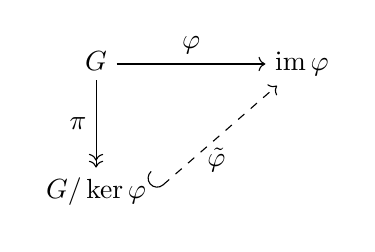
\begin{tikzpicture}
                  \matrix (m)
                        [
                        matrix of math nodes,
                        row sep    = 3em,
                        column sep = 4em
                        ]
                        {
                        G              & \im \varphi \\
                        G/\ker \varphi &             \\
                        };
                        \path
                        (m-1-1) edge [->>] node [left] {$\pi$} (m-2-1)
                        (m-1-1.east |- m-1-2)
                                edge [->] node [above] {$\varphi$} (m-1-2)
                        (m-2-1.east) edge [{Hooks[right,length=0.8ex]}->,
                                dashed] node [below] {$\tilde{\varphi}$} (m-1-2);
        \end{tikzpicture}
\end{figure}

\vspace{15pt}
\subsection{Short Exact Sequences of Groups}

\begin{defn}[Short Exact Sequence of Groups]
        A \B{short exact sequence of groups} is a diagram of five groups \begin{equation}
                1 \rightarrow H \xrightarrow{g} G \xrightarrow{f} G' \rightarrow 1
        \end{equation}
        where $f$ and $f$ are group homomorphisms, with $g$ being injective, $f$ being surjective, and $g(H) = $ kernel of $f$. Thus, H is identified with the kernel of $f$, $G'$ is identified with the image of $f$, and by the First Isomorphism Theorem, $G' \cong G/H$. (Where $1 = \{e\}$) Note that going left to right, the image of the current map is the kernel of the next.
\end{defn}
\begin{note}
        WARNING: The inputs $H$ and $G'$ do \emph{not} determine the group $G$.
\end{note}
\begin{eg}
        Take \begin{equation}
                1 \rightarrow A_3 \xrightarrow{inclusion} S_3 \xrightarrow{sign} \langle \pm 1 \rangle \rightarrow 1
        \end{equation}
        and \begin{equation}
                1 \rightarrow \Z/3\Z \cong 2\Z/6\Z \rightarrow \Z/6\Z \xrightarrow{a \mapsto a\mod 2} \Z/2\Z \rightarrow 1
        \end{equation}
        Then, since all groups of prime order are cyclic, $A_3 \cong \Z/3\Z$, and $\langle \pm 1 \rangle \cong \Z/2\Z$. However, $S_3$ is non-abelian while $\Z/6\Z$ is an abelian group of order six.
\end{eg}

\vspace{15pt}


\begin{obs}
        Suppose $H \nsub G$, and $G/H$ is the quotient group (set of cosets of $H$), which comes with a surjective canonical homomorphism $f:G \surrightarrow G/H$ by $a \mapsto aH$, with kernel $H$. \begin{enumerate}
                \item Further suppose $H \nsub K \leq G$. Then first, $H$ is normal in $K$ since $H$ is normal in $G$. Therefore, we may construct the quotient group $K/H \subset G/H$. Moreover, it is a subgroup of $G/H$. In other words, for all $aH,bH \in K/H$, $abH \in K/H$, since if $a,b \in K$, $ab \in K$. Therefore, the quotient group $K/H$ is stable under multiplication because $K$ is stable under multiplication.
                \item Conversely, any subgroup of $G$ containing $H$ corresponds to a subgroup of $G/H$ in this manner. In other words, for all subgroups $A = \{aH\}$ of $G/H$, $K = \bigcup_{aH \in A}aH = f^{-1}(A)$ is a subgroup of G containing $H$.
                \item In other words, there is a bijection between the collection of subgroups of $G$ containing $H$ and the subgroups of $G/H$.
        \end{enumerate}
\end{obs}
\begin{eg}
        Take $G = \Z$, and let $p$ be a prime number. Consider $H = p\Z$. Claim: If $\Z \geq K \geq p\Z$ is a subgroup, then either $K = \Z$ or $K = p\Z$.
        
        \begin{proof}
                Such a $K$ gives a subgroup of the cyclic quotient group $\Z/p\Z$. So, this gives either $[0]$ or $\Z/p\Z$. If it gives $[0]$, then $K = \bigcup [0] = p\Z$. Otherwise, if it gives $\Z/p\Z$, then the union of the cosets is all of $\Z$, so $K = \Z$. 
        \end{proof}

        Therefore, $H$ is a \B{maximal} subgroup of $G$.
\end{eg}


\vspace{15pt}

\subsection{Actions of a Group on Itself}


\subsubsection{Textbook}

\begin{defn}[Permutation Representation]
        Note that by definition the symmetric group on n letters, $S_n$, acts on the set $\{1,2,...,n\}$. A \B{permutation representation} of a group $G$ is a homomorphism \begin{equation}
                \phi: G\rightarrow S_n
        \end{equation}
        Given such a representation we obtain an action of $G$ on $S = \{1,...,n\}$ by letting $m_g = \phi(g)$ for all $g \in G$. In fact, actions of a group $G$ on $\{1,...,n\}$ correspond bijectively with permutation representations.
\end{defn}


\vspace{15pt}


\begin{prop}
        Suppose $G$ is a group and $S$ is a set. Then let $Perm(S)$ be the set of permutations on $S$. Then there is a bijective correspondance \begin{equation}
                \Psi: \begin{bmatrix} \text{Operations}\\\text{of $G$ on $S$}\end{bmatrix} \longleftrightarrow \begin{bmatrix} \text{homomorphisms}\\G\rightarrow Perm(S)\end{bmatrix}
        \end{equation}
        defined in this way: Given a group action, we define $\phi:G \rightarrow Perm(S)$ by the rule $\phi(g) = m_g$, where $m_g$ is the action of $g$ on elements of $S$ via left multiplication.
\end{prop}
\begin{proof}
        First, we shall provd that every element of $G$ acts on $S$ bijectively. Suppose $g \in G$, and consider te action $m_g:S\rightarrow S$. Note that by the associativity of group actions, $m_g\circ m_{g^{-1}}(s) = (gg^{-1})(s) = s$ and $m_{g^{-1}}\circ m_g(s) = (g^{-1}g)(s) = s$. Thus, $m_g$ is a bijective map on $S$, so it is a permutation of $S$. Therefore, since this is valid for all group actions, all maps $\phi:G\rightarrow Perm(S)$ is well-defined. Moreover, given a fixed group action and associated map $\phi$, we see that for all $g,g' \in G$ and for all $s \in S$, $$\phi(gg')(s) = m_{gg'}(s) = (gg').s = g.(g'.s) = m_g(m_{g'}(s)) = \phi(g)(\phi(g')(s))$$ Thus, $\phi(gg') = \phi(g)\phi(g')$, and $\phi$ is a homomorphism as claimed. Therefore, the map described above is well defined. Now, suppose $\phi:G\rightarrow Perm(S)$ is a homomorphism. Define a group action of $G$ on $S$ by declaring $g.s =\phi(g)(s)$. Since $\phi$ is a homomorphism, $\phi(e)$ is the identity map. Thus, for all $s \in S$, $e.s = \phi(e)(s) = s$. Furthermore, for all $g,g' \in G$ and $s \in S$, $(gg').s = \phi(gg')(s) = \phi(g)\circ \phi(g')(s) = g.(g'.s)$. Therefore, it is a well defined group action, and $\Psi($group action$)=\phi$. Thus, $\Psi$ is surjective. Next, suppose $G_1,G_2$ are group actions such that $\Psi(G_1) = \Psi(G_2)$. Then $\phi_1 = \phi_2$, so for all $g \in G$, $\phi_1(g) = \phi_2(g)$. Finally, this implies that for all $g \in G$ and $s \in S$, $g._1s = g._2s$. Therefore, every element of $G$ acts in the same way on $S$ when using the $G_1$ and $G_2$ group action structures. Consequently, $G_1 = G_2$ and $\Psi$ is a bijective map, as claimed.
\end{proof}


\vspace{15pt}



\begin{defn}[Faithful]
        If the homomorphism $\phi:G\rightarrow Perm(S)$ is injective, then the corresponding group action is said to be \B{faithful}. Hence, to be faithful, the action must have the property that $m_g \neq $ identity unless $g=1$, or \begin{equation}
                \forall s \in S, gs = s \implies g=1
        \end{equation}
\end{defn}



\vspace{15pt}


\begin{defn}[Group Action on Itself]
        A group action of a group $G$ on itself is equivalent to the group action on a set, where now the set is the group. Thus, it is a map \begin{equation}
                G\times G \rightarrow G
        \end{equation}
        such that for all $g,g',g'' \in G$, $e(g) = g$, and $(g'g'')(g) = g'(g''(g))$.
\end{defn}

\vspace{15pt}


\begin{eg}
        Suppose $G$ is a group. A common group action of $G$ on itself is Left multiplication: $g.g' \mapsto gg'$. Note that this is evidently a transitive operation on $G$ since $O_e = G$. Additionally, for any $g \in G$, $G_g = \{e\}$. Thus, the action is faithful and the homomorphism \begin{equation}
                        G\rightarrow Perm(S)
        \end{equation} 
        given by $g\mapsto m_g = $ left multiplication by $g$.
\end{eg}


\vspace{15pt}

\begin{thm}[Cayley's Theorem]
        Every finite group $G$ is isomorphic to a subgroup of the permutation group. If $G$ is of order $n$, then it is isomorphic to a subgroup of the symmetry group $S_n$.
\end{thm}
\begin{proof}
        Since the operation by left multiplication is faithful, $G$ is isomorphic to its image $Perm(G)$. If $G$ is of order $n$, then $Perm(G)$ is isomorphic to $S_n$. (??)
\end{proof}

\vspace{15pt}

\begin{eg}[Conjugation]
        Suppose $G$ is a group. Another common group action of $G$ on itself is \B{conjugation}, so the map $G\times G\rightarrow G$ is defined by \begin{equation}
                (g,x) \mapsto gxg^{-1}
        \end{equation}
        Obviously any element conjugated by the identity is itself. Moreover, a map defined by conjugation is a homomorphism so the action is associative.
\end{eg}

\vspace{15pt}


\begin{defn}[Centralizer]
        The stabilizer of an element $x \in G$ under the action of conjugation is called the \B{centralizer} of $x$, and is denoted by $Z(x):$ \begin{equation}
                Z(x):= \{g \in G: gxg^{-1} = x\}
        \end{equation}
        Thus, the centralizer of $x$ is the set of all elements which commute with $x$. Note that $x \in Z(x)$ since $x$ commutes with itself.
\end{defn}

\vspace{15pt}

\begin{defn}[Class Equation]
        The orbit of $x$ for the action of conjugation is called the \B{conjugacy class} of $x$. It consists of all conjugate elements $gxg^{-1}$. We often denote the conjugacy class by \begin{equation}
                C_x = \{x' \in G:\exists g\in G, x' = gxg^{-1}\}
        \end{equation}
        By the counting formula we have that \begin{equation}
                |G| = |C_x||Z(x)|
        \end{equation}
\end{defn}


\vspace{15pt}


\begin{defn}[Class Equation]
        Note that since conjugacy classes are orbits for a group action, $G$ is partitioned by the conjugacy classes. Then for a finite group $G$ we have the \B{Class Equation} \begin{equation}
        |G| = \sum\limits_{\begin{array}{c} conjugacy \\ classes\;C\end{array}}|C|
\end{equation}
\end{defn}


\vspace{15pt}


\begin{obs}
        Note that on the right of the class equation we have orders of conjugacy classes, or orbits, which divide the group. Additionally, the conjugacy class of the identity is simply $\{e\}$, so at least one element on the right side is 1.
\end{obs}


\vspace{15pt}


\begin{rec}
        Recall that the center of a group $G$ is the set $Z$ of elements in $G$ which commute with every element in $G$. Thus, the conjugacy class of any element in the center is a set consisting of only that element.
\end{rec}


\vspace{15pt}

\begin{prop}
        An element $x$ is in the center of the group $G$ if and only if its centralizer $Z(x)$ is the entire group.
\end{prop}


\vspace{15pt}

\begin{prop}
        Suppose $G$ is a \B{p-group}, so $|G| = p^k$, where $p$ is prime, and $k \in \N$. Then the center of $G$ has order $> 1$.
\end{prop}
\begin{proof}
        Suppose $G$ is a p-group, so $|G| = p^n$ for some $n \in \N$. Then every conjugacy class has order which divides $p^n$, so they are all powers of $p$. Note that $|C_1| = 1$. For the sake of contradiction suppose that no other conjugacy class of order 1 exists. Then \begin{equation}
                p^n = 1 + \sum(powers\;of\;p)
        \end{equation}
        However, this is impossibly unless $n = 0$. Therefore, the center of $G$ has order $> 1$, as desired.
\end{proof}


\vspace{15pt}

\begin{prop}
        Let $G$ be a p-group, and let $S$ be a finite set on which $G$ acts. Assume that the order of $S$ is not divisible by $p$. Then there is a fixed point for the action $G$ on $S$, that is, an element $s \in S$ is stabilized by every element of $G$, so $Z_s = G$.
\end{prop}

\vspace{15pt}

\begin{prop}
        Every group of order $p^2$ is abelian.
\end{prop}



\begin{proof}
        Let $G$ be a group of order $p^2$. We shall show that for all $x \in G$, the centralizer $Z(x)$ is the whole group. Let $x \in G$. If $x$ is in the center $Z$, then $Z(x) = G$ as claimed. If $x \notin Z$, then $Z(x)$ is strictly larger than $Z$ since it contains $Z$ and $x$. Now, the orders of $Z$ and $Z(x)$ divide $|G|=p^2$, and from a previous proposition we know that $|Z|$ is at least $p$. The only possibility is then $|Z(x)| = p^2$. Hence, $Z(x) = G$, and $x$ is in the center, which is a contradiction. Therefore, $x \in Z$ for all $x \in G$, so $Z = G$ and $G$ is correspondingly abelian.
\end{proof}


\vspace{15pt}


\begin{cor}
        Every group of order $p^2$ is one of the following types: \begin{enumerate}
                \item a cyclic group of order $p^2$
                \item a product of two cyclic groups of order p
        \end{enumerate}
\end{cor}
\begin{proof}
        Since the order of an element divides $p^2$, there are two cases two consider \begin{enumerate}
                \item[] Case 1: $G$ contains an element of order $p^2$, then $G$ is cyclic.
                \item[] Case 2: Every element $x \in G$ except the identity is of order $p$. Let $x,y \in G$, $x,y \neq 1$, and let $H_1$ and $H_2$ be cyclic subgroups generated by $x$ and $y$ respectively. We may choose $y$ so that it is not a power of $x$. Then since $y \notin H_1$, $H_1 \cap H_2$ is smaller than $H_2$, which is of order $p$. Thus, $H_1 \cap H_2 = \{1\}$. Also, since $G$ is abelian, the subgroups are normal. Since $y \notin H_1$, the group $H_1H_2$ is strictly larger than $H_2$, and its order divides $p^2$. Thus, $H_1H_2 = G$. By a previous result, it follows that $G \cong H_1 \times H_2$
        \end{enumerate}
\end{proof}


\vspace{15pt}

\begin{rec}
        Recall that the order of the icosahedral group is $60$. Each of the twenty vertices have a stabilizer of order 3, with opposite vertices sharing the same stabilizer, giving 10 subgroups of order 3, and all of these subgroups only have the identity in common. The twelve faces each have stabilizers of order 5, and since a stabilizer is shared between opposite pairs of faces, we have 6 subgroups of order 5. Finally, there are 15 stabilizers of edges, with elements of order 2. Then, the 1 identity element of order 1, giving the class equation \begin{equation}
                60 = 1 + 15 + 20 + 24
        \end{equation}
        Moreover, this equation is split up by conjugacy classes as \begin{equation}
                60 = 1 + 15 + 20 + 12 + 12 
        \end{equation}
\end{rec}


\vspace{15pt}

\begin{rec}
        Recall that is a group $G$ acts on a set $S$, and for $s,s' \in S$, $s' \in O_s$, and $s' = gs$ for $g \in G$, the stabilizers of $s$ and $s'$ are conjugate, and in particular $G_{s'} = gG_sg^{-1}$.
\end{rec}

\vspace{15pt}

\begin{thm}
        The icosahedral group $I$ has no proper normal subgroups.
\end{thm}
\begin{proof}
        A proper normal subgroup of $I$ has order which is a proper divisor of 60. Moreover, the order of the subgroup is the sum of some of the terms $1,15,20,12,12$, including $1$. No such integer exists, so no proper normal subgroup of $I$ exists. Therefore, $I$ is simple.
\end{proof}



\vspace{15pt}


\begin{lem}
        .\newline \begin{enumerate}
                \item If a normal subgroup $N$ of a group $G$ contains an element $x$, then it contains the conjugacy class $C_x$ of $x$ in $G$. In other words, a normal subgroup is a union of conjugacy classes.
                \item The order of a normal subgroup $N$ of $G$ is the sum of the orders of the conjugacy classes of which it contains.
        \end{enumerate}
\end{lem}

\begin{proof}
        Suppose that $G$ is a group, and $N$ is a normal subgroup of $G$. Let $x \in N$. Then given an element $y \in C_x$, $y$ is of the form $y = gxg^{-1}$ for some $g \in G$. Then, since $N$ is normal, $y = gxg^{-1} \in N$, which implies that $C_x \subset N$. Then, since conjugacy is an equivalence relation, the distinct conjugacy classes of elements in $N$ partition the group, so \begin{equation}
                |N| = \sum\limits_{\begin{array}{c}conjugacy\\classes\;C\end{array}}|C|
        \end{equation}
\end{proof}


\vspace{15pt}

\begin{thm}
        The icosahedral group is isomorphic to the alternating group $A_5$. (we have $I$ operate on inscribed cubes of the dodecahedron)
\end{thm}

\vspace{15pt}

\subsubsection{Lecture}

\begin{rec}[Class equation Results]
        Any $G$ of order $p^2$ is abelian. (from before, any $G$ of order $p$ is cyclic $(\cong \Z/p\Z)$).
\end{rec}

\vspace{15pt}

\begin{qst}
        What about $G$ of order $pq$ (ex: $S_3$ of order 6), or $p^3$?
\end{qst}

\vspace{15pt}

\begin{prop}
        If $G$ is a group of order $p^2$, then there are only two such $G$ up to isomorphism: \begin{enumerate}
                \item There is an element of $G$ of order $p^2$. Then $G \cong \Z/p^2\Z$ with the map \begin{equation}
                                g\mapsto 1 (\mod p^2), g^a \mapsto a (\mod p^2)
                \end{equation}
        \item There is no element of $G$ of order $p^2$. Thus, every $g \neq e$ has order $p$. Then, the field $\Z/p\Z$ acts on the group $G$ by \begin{equation}
                        a\cdot g = g^a = g+g+...+g\;(a\;times)
        \end{equation}
                        where $a \in \Z/p\Z$, and $0\cdot g = e = 0$ in the additive group. In this case, $G$ is a vector space over $\Z/p\Z$, it has order $p^2$, so it has dimension $2$, and it is isomorphic to $(\Z/p\Z)^2$ by a choice of a basis. In sum, if every element has order $p$, then you obtain an action of the field $\Z/p\Z$ on the group, which turns it into 2-dimensional a vector space.
        \end{enumerate}
\end{prop}

\vspace{15pt}

\begin{defn}[Elementary Abelian P-group]
        For $n\geq 1$, we have the group $G = (\Z/p\Z)^n$, an n-dimensional vector space over $\Z/p\Z$, with order $p^n$, and every element $g \neq e$ of order $p$. This is called an \B{elementary abelian p-grop}.
\end{defn}

\vspace{15pt}



\subsection{Operations on Subsets}

\subsubsection{Textbook}

\begin{defn}[Action on Subsets]
        Suppose $G$ is a group that acts on a set $S$. Let $U \subset S$ be a subset of $S$. Then \begin{equation}
                gU = \{g.u:u \in U\}
        \end{equation}
        is another subset of $S$. Then $G$ operates on the set of subsets of $S$. If we wish we can consider the action on subsets of a given order, since multiplication by $g \in G$ permutes $S$, so the subsets $U$ and $gU$ will be of the same order.
\end{defn}

\vspace{15pt}

\begin{eg}
        Let $O$ be the octahedral group of 24 rotations of a cube, and let S be the set of vertices of the cube. Consider the operation $O$ on subsets of order 2 of $S$. There are 28 such subsets, and they form three orbits for the group \begin{enumerate}
                \item $\{$pairs of vertices on an edge$\}$
                \item $\{$pairs which are opposite on a face of the cube$\}$
                \item $\{$pairs which are opposite on the cube$\}$
        \end{enumerate}
        These orbits have orders of 12, 12 and 4 respectively.
\end{eg}

\vspace{15pt}

\begin{defn}[Stabilizer of a Subset]
        The stabilizer of a subset $U$ is the set of group elements $g \in G$ such that $gU=U$. However, note that the equality does not mean that $g$ leaves the points of $U$ fixed, but rather that $g$ permutes the elements within $U$, that is $g.u\in U$ whenever $u \in U$.
\end{defn}

\vspace{15pt}

\begin{prop}
        Let $H$ be a group which operates on a set $S$, and let $U$ be a subset of $S$. Then $H$ stabilizes $U$ if and only if $U$ is the union of $H-orbits$.
\end{prop}
\begin{proof}
        If $H$ stabilizes $U$, then the $H-orbit$ of every element in $U$ must be contained in $U$. Thus, $U$ is the union of the $H-orbits$ of its elements. Conversely, if $U$ is the union of $H-orbits$, then for each $u \in U$, $O_u \in U$, so $H$ stabilizes $U$ by definition.
\end{proof}

\vspace{15pt}


\begin{prop}
        Let $U$ be a subset of a group $G$. The order of the stabilizer $Stab(U)$ of $U$ for the operation of left-multiplication divides the order of $U$.
\end{prop}
\begin{proof}
        Let $H$ denote the stabilizer of $U$. The previous proposition tells us that $U$ is a union of $H-orbits$ for action of $H$ on $G$. These orbits are right cosets of the form $Hg$ for all $g \in G$. Thus, $U$ is the union of right cosets. Hence, the order of $U$ is a multiple of $|H|$.
\end{proof}

\vspace{15pt}

\begin{rmk}
        Since the stabilizer is a subgroup of $G$, $|Stab(U)|$ divides $|G|$ and $|U|$, so if $|G|$ and $|U|$ are relatively prime, then $|Stab(U)|$ is the trivial subgroup, $\{e\}$.
\end{rmk}

\vspace{15pt}


\begin{defn}[Conjugate Subgroup]
        For a subgroup $H \subset G$ of a group $G$, the orbit under conjugation of $H$ is the set of \B{conjugate subgroups}\begin{equation}
                \{gHg^{-1}: g \in G\}
        \end{equation}
        Consequently, the subgroup $H$ is normal if and only if its orbit under conjugation consists of $H$ alone, that is, $gHg^{-1} = H$ for all $g \in G$.
\end{defn}

\vspace{15pt}

\begin{defn}[Normalizer]
        The stabilizer of a subgroup $H$ under the action of conjugation is known as the \B{normalizer} of $H$, and is denoted by \begin{equation}
                N(H) := \{g \in G: gHg^{-1} = H\}
        \end{equation}
\end{defn}


\vspace{15pt}


\begin{thm}[Counting Formula]
        The \B{counting formula} for conjugation on subgroups is \begin{equation}
                |G| = |N(H)|\cdot|\{conjugate\;subgroups\}|
        \end{equation}
        Thus, the number of conjugate subgroups is equal to the index $[G:N(H)]$.
\end{thm}


\vspace{15pt}

\begin{rmk}
        Note that the normalizer always contains the subgroup \begin{equation}
                H \subset N(H) 
        \end{equation}
        because $hHh^{-1} = H$ when $h \in H$. Thus, by Lagrange's Theorem, $|H|$ divides $|N(H)|$, and $|N(H)|$ divides $|G|$.
\end{rmk}

\vspace{15pt}

\begin{rmk}
        The definition of a normalizer $N(H)$ implies that $H \nsub N(H)$, and in fact, $N(H)$ is the largest subgroup of $G$ containing $H$ as a normal subgroup. In particular, $N(H) = G$ if and only if $H$ is a normal subgroup of $G$.
\end{rmk}

\vspace{15pt}

\subsection{The Sylow Theorems}


\subsubsection{Textbook}

In this section we consider a group $G$ of order $n$. Let $p$ be a prime which divides $n$, and write \begin{equation}
        n=p^em
\end{equation}
where $e \geq 1$, and $\gcd(p,m) = 1$ for some integer $m$. 

\begin{thm}[First Sylow Theorem]
        There is a subgroup of $G$ whose order is $p^e$, which we call a \B{Sylow p-subgroup}.
\end{thm}

\vspace{15pt}

\begin{cor}
        If a prime $p$ divides the order of a finite group $G$, then $G$ contains an element of order $p$.
\end{cor}
\begin{proof}
        Let $H$ be a supgroup of order $p^e$, and let $x$ be an element of $H$ different from $1$. The order of $x$ divides $p^e$, so it is $p^r$ with $0 < r \leq e$. Then $x^{p^{r-1}}$ has order $p$.
\end{proof}

\vspace{15pt}

\begin{cor}
        There are exactly two isomorphism classes of groups of order $6$. They are classes of the cyclic group $C_6$ and of the dihedral group $D_6$
\end{cor}
\begin{proof}
        Let $x$ be an element of order $3$ and $y$ an element of order $2$ in $G$. It can be seen that the six products $x^iy^j$, $0\leq i \leq 3, 0 \leq j \leq 2$ are distinct elements of $G$. For, we can write $x^iy^j=x^ry^s$ in the form $x^{i-r}=y^{s-j}$. Every power of $x$ except the identity has order $3$, and every power of $y$ except the identity has order $2$. Thus, $x^{i-r} = y^{s-j} = 1$, which shows that $r=i$ and $j=s$. Since $G$ has order $6$, the six elements we have shown are distinct run through the whole group. Moreover, $yx$ must be one of these products, and in particular, $yx = xy$ or $yx =x^2y$ holds in $G$. Either of these relations along with $x^3 = 1$ and $y^2 =1$ provides a valid multiplication table for the group. Therefore, there are at most two isomorphism classes for the group. $C_6$ and $D_6$ are the only such groups.
\end{proof}

\vspace{15pt}


\begin{defn}[Sylow p-subgroups]
        Let $G$ be a group of order $n = p^em$, where $p$ is a prime, $\gcd(m,p) = 1$, and $e \geq 1$. The subgroups $H$ an $G$ of order $p^e$ are called \B{Sylow p-subgroups} of $G$, or often just \B{Sylow subgroups}.
\end{defn}


\vspace{15pt}

\begin{thm}[Second Sylow Theorem]
        Let $K$ be a subgroup of $G$ whose order is divisible by $p$, and let $H$ be a Sylow p-subgroup of $G$. There is a conjugate subgroup $H' = gHg^{-1}$ such that $K \cap H'$ is a Sylow subgroup of $K$.
\end{thm}


\vspace{15pt}

\begin{cor}
        .\newline \begin{enumerate}
                \item If $K$ is any subgroup of $G$ which is a p-group, then $K$ is contained in a Sylow p-subgroup of $G$
                \item The Sylow p-subgroups are all conjugate.
        \end{enumerate}
\end{cor}
\begin{proof}
        First, note that conjugation is an automorphism of subgroups, so the conjugate of a Sylow p-subgroup is another Sylow p-subgroup. First, note that the Sylow subgroup of the p-group $K$ is $K$ itself. Thus, if $H$ is a Sylow subgroup and $K$ is a p-group, there is a conjugate $H'$ such that $K\cap H' = K$, which is to say that $H'$ contains $K$ (by the Second Sylow Theorem). For the second part, let $K$ and $H$ be Sylow subgroups. Then there is a conjugate $H'$ of $H$ such that $H' \cap K$ is a Sylow subgroup of $K$. Then since $K$ is a Sylow subgroup, $H' \cap K = K$, and hence $K \subset H'$. Moreover, since $|K| = |H'|$ as they are both Sylow subgroups, $K = H'$. Thus, $K$ and $H$ are conjugate.
\end{proof}

\vspace{15pt}

\begin{thm}[Third Sylow Theorem]
         Let $|G| = n$, and $n = p^em$ as initially stated. Let $s$ be the number of Sylow p-subgroups. Then $s$ divides $m$ and is congruent to $1$ modulo $p$: $s\;\vert\;m$, and $s = ap + 1$ for some $a \geq 0$.
\end{thm}


\vspace{15pt}


\begin{prop}
        .\newline \begin{enumerate}
                \item Every group of order $15$ is cyclic.
                \item There are two isomorphism classes of groups of order $21$: the class of the cyclic group $C_{21}$, and the class of the group $G$ having two generators $x,y$ which satisfy the relation $x^7=y^3=1,$ $yx = x^2y$.
        \end{enumerate}
\end{prop}
\begin{proof}
        \begin{enumerate}
                \item Let $G$ be a group of order $15$. By the Third Sylow Theorem, the number Sylow 3-subgroups of $G$ divides $5$ and is congruent to 1 modulo 3. The only such integer is $1$. Therefore, there is only one Sylow 3-subgroup $H$, and thus the conjugacy class of $H$ must be of order 1, so $H$ is normal. Similarly, there is one Sylow 5-subgroup of $G$, which we shall denote by $K$. $K$ must also be a normal subgroup of $G$. Then, since $K\cap H$ is a subgroup of $H$ and $K$, its order divides 5 and 3 so $K \cap H = \{e\}$. Also, $KH$ is a subgroup of order $> 5$, so $KH = G$. By a previous result, $G$ is isomorphic to the product group $H\times K$. Thus, every group of order $15$ is isomorphic to the direct product of two cyclic groups of orders 3 and 5. In particular, since $C_{15}$ is of order $15$, it is also isomorphic to the product, so every group of order 15 is cyclic.
                \item Let $G$ be a group of order $21$. Then, the Third Sylow Theorem shows that the single Sylow 7-subgroup $K$ must be normal. But, we have the possibility there are 7 Sylow 3-subgroups of $G$. Let $x$ denote a generator for $K$, and $y$ a generator for one of the Sylow 3-subgroups $H$. Then $x^7 = y^3 = 1$, and since $K$ is normal, $yxy^{-1} = x^i$ for some $i < 7$. Using the fact that $y^3 = 1$, we see that \begin{equation}
                                x = y^3xy^{-3} = x^{i^3}
                \end{equation}
                        Therefore, $i^3$ is congruent to 1 modulo $7$. This implies that $i$ is either 1, 2, or 4.
                        \begin{enumerate}
                                \item[] Case 1: $yxy^{-1} = x$. Then the group is abelian and by a previous result it is congruent to a direct product of cyclic groups of orders 3 and 7. Such a group is cyclic.
                                \item[] Case 2: $yxy^{-1} = x^2$. The multiplication of $G$ can be carries out using the rules $x^7=y^3 = 1$, $yx = x^2y$, to reduce every product of elements $x$ and $y$ to one of the form $x^iy^j$, $0\leq i < 7, 0 \leq j < 3$. (prove existence)
                                \item[] Case 3: $yxy^{-1} = x^4$. In this case we replace $y$ by $y^2$, which is also a generator for $H$, to reduce to the previous case: $y^2xy^{-2} = x^2$. Thus, there are two isomorphism classes of the group of order $21$ as claimed.
                        \end{enumerate}
        \end{enumerate}
\end{proof}


\vspace{15pt}


\begin{rmk}[Proofs of the Sylow Theorems]
        We shall now prove the Sylow Theorems.
\end{rmk}
\begin{proof}
        [\B{First Sylow Theorem}] We let $\mathcal{J}$ be the set of all subsets of $G$ of order $p^e$. We shall show that one of these subgroups has a stabilizer of order $p^e$. The stabilizer will be the required subgroup. 

        \begin{lem}
                The number of subsets of order $p^e$ in a set of $n = p^em$ elements, with $\gcd(p,m) = 1$, is the binomial coefficient \begin{equation}
                        N = \binom{n}{p^e} = \frac{n(n-1)...(n-k)...(n-p^e+1)}{p^e(p^e-1)...(p^e-k)...1}
                \end{equation}
                Moreover, $\gcd(N,p) =1$.
        \end{lem}
        \begin{proof}
                [Proof of Lemma] Is is a standard fact that the number of subsets of a set of order $p^e$ is this binomial coefficient. To see that $N$ is not divisible by $p$, note that every time $p$ divides a term $(n-k)$ in the numerator of $N$, it also divides the term $(p^e-k)$ in the denominator exactly the same number of times: If we write $k$ in the form $k =p^il$, where $\gcd(p,l) = 1$, then $i < e$. Therefore, $(n-k)$ and $(p^e - k)$ are both divisible by $p^i$ but not divisible by $p^{i+1}$, satisfying the claim.
        \end{proof}


        We decompose $\mathcal{J}$ into orbits for the action of left multiplication, obtaining the formula \begin{equation}
                N = |\mathcal{J}| = \sum\limits_{orbits\;O}|O|
        \end{equation}
        Since $p$ does not divide $N$, some orbit has an order not divisible by $p$, say the orbit of the subset $U$. Then, $G$ acts transitively on the orbit $O_U$, so by the Counting Formula \begin{equation}
                |Stab(U)|\cdot|O_U| = |G| = p^em
        \end{equation}
        Since $|O_U|$ is not divisible by $p$, we have that $p^e$ divides $|Stab(U)|$, so $p^e \leq |Stab(U)|$. Moreover, if $g \in Stab(U)$, then $gU = U$. This implies that $U$ is the union of right cosets of $Stab(U)$. In particular, $|Stab(U)| \leq |U| = p^e$, so we conclude that $|Stab(U)| = p^e$, completing the proof. 
\end{proof}
\vspace{15pt}

\begin{proof}
        [\B{Second Sylow Theorem}] We are given a subgroup $K$ of order divisible by $p$, and a Sylow subgroup $H$ of $G$, and we are to show that for some conjugate $H'$ of $H$, the intersection $K\cap H'$ is a Sylow subgroup of $K$.


        Let $S$ denote the set of left cosets $G/H$. Note that $G$ operates transitively on $S$, so the set forms a single orbit, and that $H$ is the stabilizer of the element $s= eH$ of $S$. Thus, the stabilizer of $as$ is the conjugate subgroup $aHa^{-1}$.


        We restrict the group action of $G$ to $K$, and decompose $S$ into $K-orbits$. Since $H$ is a Sylow subgroup, the order of $S$ is prime to $p$. Thus, there must exist some $K-orbit$ $O$ whose order is prime to $p$. Say that $O$ is the $K-orbit$ of the element $as$. Let $H'$ denote the stabilizer $aHa^{-1}$ of $as$ for the operation of $G$. Then, the stabilizer of $as$ for the restricted action of $K$ is $H'\cap K$, and the index $[K:H'\cap K]$ is $|O|$, which is prime to $p$. Also, since it is a conjugate of $H$, $H'$ is a p-group. Therefore, $H' \cap K$ is a p-group. Thus, $H' \cap K$ is a p-group of the largest order in $K$, so $H' \cap K$ is a Sylow subgroup of $K$.
\end{proof}

\vspace{15pt}

\begin{proof}
        [\B{Third Sylow Theorem}] By a corollary of the Second Sylow Theorem above, we have that the Sylow subgroups of $G$ are all conjugate to one another. In particular, they are all conjugate to a given one, say $H$. Thus, the orbit of $H$ by conjugation by $G$ is the conjugacy class of all Sylow subgroups, and $s = [G: N(H)]$ is the number of Sylow subgroups, where $N(H)$ is the normalizer of $H$ in $G$ under conjugation. Since $H \subset N(H)$, $H$ is a subgroup of $N(H)$ and $p^e$ divides $|N(H)|$ Moreover, note that $[G:H] = m$, and $[G:N(H)] = \frac{[G:H]}{k}$ for some $k > 0$, so in particular, $s = [G:N(H)]$ divides $m$. To show $s \equiv 1 (\mod p)$, we decompose the set $\{H_1,H_2,...,H_s\}$ of Sylow subgroups into orbits for the operation of conjugation by $H = H_1$. An orbit consists of a single group $H_i$ if and only if $H$ is contained in the normalizer $N(H_i)$ of $H_i$. If so, then $H$ and $H_i$ are both Sylow subgroups of $N(H_i)$, and $H_i$ is normal in $N(H_i)$. Then, by a previous corollary to the Second Sylow Theorem, $H$ and $H_i$ are conjugate in $N(H_i)$, but $H_i$ is only conjugate with itself in $N(H_i)$. Therefore, $H = H_i$. Thus, $H$ is the only Sylow subgroup with $H-orbit$ of order 1. The other orbits have orders divisible by $p$ since their orbits divide $|H|$, by the Counting Formula. Thus, $s \equiv 1 (\mod p)$, completing the proof.
\end{proof}


\vspace{15pt}



\subsubsection{Lecture}

\begin{defn}[Operation of a Group on itself by Conjugation]
        $G$ acts on $G = S$ by conjugation \begin{equation}
                g(s)\mapsto gsg^{-1}
        \end{equation}
        The orbit $O_s$ is called the \B{conjugacy class} of the element $s$, and the stabilizer $G_s$ is called the \B{centralizer} of $s$, written usually as $Z_s := \{ g \in G: gsg^{-1} =s \}$
\end{defn}

\vspace{15pt}

\begin{defn}[Action on Subgroups]
        $G$ also acts on the set $\mathcal{H}$ of all subgroups of $G$, by conjugation. In particular, for all $g \in G$ and $H \in \mathcal{H}$, $g(H) = gHg^{-1} = \{ghg^{-1}: h \in H$ another element of $\mathcal{H}$. The orbit of $H$, $O_H = $ the set of subgroups conjugate to $H$, and the stabilizer of $H$ is the subgroup $G_H = \{g \in G: gHg^{-1}\} = N(H) \subset G$, which we call the \B{normalizer} of $H$. Note that $N(H)$ is a subgroup such that $H \nsub N(H) \subset G$. Moreover, $N(H)$ is the largest subgroup of $G$ containing $H$ in which $H$ is normal.
\end{defn}

\vspace{15pt}

\begin{rmk}
        For a group $G$ we have so far had the notion of $G$ acting on sets, $G$ acting on the set of its own elements, and now $G$ acting on the set of subgroups of $G$.
\end{rmk}


\vspace{15pt}


\begin{eg}[Examples of Normalizers]
        Consider $S_3$ and the normal subgroup $A_3 = \{e, (1\;2\;3),(1\;3\;2)\}$, so $N(A_3) = S_3$. On the other hand $\{e,(1\;2)\} \subset S_3$ since $(1\;2)$ is the only element of order two, not only must a normalizer normalize $(1\;2)$ (keep it in the subgroup) it must also centralize it (not change it - i.e. commute with it). However, there is no such element except for the elements already in $\{e,(1\:2)\}$, so $N(\{e,(1\;2)\}) = \{e,(1\;2)\}$.


        Let us consider the subgroup \begin{equation}
                H = \left\{\begin{bmatrix} 1 & b \\ 0 & 1 \end{bmatrix}\right\} \subset G = GL_2(F)
        \end{equation}
        Then the normalizer of $H$ is \begin{equation}
                N(H) = \left\{\begin{bmatrix} a & b \\ 0 & c \end{bmatrix}\right\} 
        \end{equation}
\end{eg}

\vspace{15pt}

\begin{rmk}[Stabilizers]
        Recall that if we have $G$ acting transitively on a set $S$, and $G_s$ is the stabilizer of some element $s \in S$, then $G_s$ is conjugate to the stabilizer $G_{s'}$ for all $s' \in S$. Thus, the stabilizers generate a conjugacy class of subgroups.
\end{rmk}

\vspace{15pt}

\begin{rmk}[Normalizer WARNING]
        A normalizer does not necessarily centralize the elements of the set it normalizes (i.e. fixes them). All it guarantees is that for any element $g$ in the normalizer $G_H$ of a subgroup $H$, $ghg^{-1} \in H$ for all $h \in H$.
\end{rmk}

\vspace{15pt}

\begin{rmk}[FACT]
        If $N = p^mn$, where $p$ is prime, then \begin{equation}
                \binom{N}{p^m} = \frac{N!}{p^m(N-p^m)!} = \frac{(p^mn)!}{p^m(p^m(n-1))!} = \frac{N(N-1)...(N-p^m+1)}{p^m(p^m-1)...1}
        \end{equation}
        is prime to $p$. Since the power of $p$ dividing the numemrator $=$ the power of $p$ dividing the denominator (Order of $p$). In general, the power of of $p$ dividing $(N-k)$ is equal to the power of $p$ dividing $(p^m-k)$, with $k < p^m$ (i.e. $ord_p(N-k) = ord_p(p^m - k)$). This follows from the fact that the same power of $p$ divides $N$ and $p^m$, so all we need to look at is the $k$ which is the same for both.
\end{rmk}


\vspace{15pt}

\begin{thm}[Sylow Theorem]
        Assume $G$ is a finite group of order $N = p^m\cdot n$, where $p$ is prime, and $\gcd(n,p) = 1$, so $p^m$ is the highest power of $p$ which divides the group. Then, \begin{enumerate}
                \item There is a subgroup $H$ of $G$ of order $p^m$ (\B{Sylow p-subgroups})
                \item If $K$ is a subgroup (p-group) of order $p^a$ ($a \leq m$), then $K$ is contained in a conjugate of $H$. In particular, any two p-Sylow subgroups $H$ and $H'$ are conjugate (the case when $a = m$). $\implies$ thus the Sylow p-subgroups form a conjugacy class of subgroups.
                \item The number $l$ of Sylow p-subgroups of $G$ (in this single conjugacy class) divides $n$, and satisfies \begin{equation}
                                l \equiv 1 (\mod p)
                \end{equation}
        \end{enumerate}
\end{thm}
\begin{proof}[Part 1]
        Let $G$ act on the set $S$ of all subsets of $G$ which have order $p^m$ by translation ($J\subset G$ goes to $gJ \subset G$ by left translation). Moreover, $|S| = \binom{N}{p^m}$, which from above is prime to $p$. We will realize $H$ as a stabilizer $G_s$ for this action. We break $S$ into $G-orbits$, so \begin{equation}
                |S| = |O_{s_1}| + ... + |O_{s_r}| = \frac{|G|}{|G_{s_1}|} + ... + \frac{|G|}{|G_{s_n}|}
        \end{equation}
        where  $G$ acts transitively on each orbit. Since $|S|$ is prime to $p$, there is at least one orbit of order prime to $p$. Say $|O_s|$ is prime to $p$, $s \in \{s_1,...,s_n\}$. Since $|O_s| = \frac{p^mn}{|G_s|}$ is prime to $p$, we must have that $p^m$ divides $|G_s|$. I claim that $|G_s| \leq p^m$. $s$ corresponds to a subset $J \subset G$, and we have an element of the stabilizer of that subset. If $g \in G_s$, then $gJ = J$. This implies that $J$ is a union of left cosets of $G_s$. In particular ,$|G_s| \leq |J| = p^m$. In fact, $J$ has stabilizer of order $p^m$ if and only if $J = H$ is a Sylow p-subgroup, in which case $J = G_s = H$.
\end{proof}
\begin{proof}[Part 2]
        Suppose $H$ is the Sylow p-subgroup found in part 1. Suppose $G$ acts transitively on $S = G/H$, which has order $n$ prime to $p$. The stabilizers of any point $s = sH$ in $S$, $G_s$, are the conjugates of $H$. Let $K$ be another $p$-subgroup, and have $K$ act by the restriction of the $G$ action on $S$. Since the order of $S$ is of order prime to $p$, there must be an orbit $sH$ of order prime to $p$. It follows that $|K|/|stabilizer|$ is prime to $p$. Note that the order of $K$ is a power of $p$, so the only option is that the order of the stabilizer is equal to the order of $K$. Thus, there must be an orbit fixed by $K$. Recall that $Stab_{sH} = K \cap G_s = K \cap sHs^{-1}$, and since the orders are equal it follows that $K \subset sHs^{-1}$. This shows that our p-group must be contained in some conjugate of our Sylow $p$ subgroup.
\end{proof}
\begin{proof}[Part 3]
        We claim the number of Sylow subgroups, $l$, is $|G|/|N(H)|$, where $H$ is a Sylow p-subgroup, because $G$ acts transitively on the set of Sylow p-subgroups by conjugation (by part 2), and the stabilizer of $H$ is what we call $N(H)$. Moreover, since $H \subset N(H)$, so $|N(H)|$ is divisible by $p^m$, so $l$ divides what's left, which is $n = N/p^m$. Now, restrict the action of conjugation on the $l$ Sylows to the subgroup $H$. The orbit of $H$ has 1-element, and all other orbits have $p^a $ elements, with $a \geq 1$. Since $|H| = p^m$, the size of any orbit must divide this. For the sake of contradiction, suppose $H'$ is another Sylow p in an orbit of size $1$, then $H$ normalizes $H'$. Thus $H$ and $H'$ are both subgroups of $N(H')$. Therefore, since we also have that $N(H') \subset G$, $|N(H')| = p^mn'$, where $n'$ divides $n$. Moreover, $H$ and $H'$ are Sylow p-subgroups of $N(H')$. Then, by part 2, they are conjugate in $N(H')$. But, in $N(H')$ the only thing conjugate to $H'$ is $H'$. Thus, we conclude that $H' = H$.
\end{proof}




\vspace{15pt}

\begin{rmk}
        If $d$ divides the order $N$ of $G$, there need \emph{not} be a subgroup of order $d$. For example, if $G = A_4$, it has order $12$, but no subgroup of order $6$.
\end{rmk}


\vspace{15pt}

\begin{thm}[Sylow Theorems Restated]
        If $G$ is finite of order $N=p^nm$ with $\gcd(p,m) = 1$, the \begin{enumerate}
                \item There exists Sylow p-subgroups of order $p^n$
                \item Any two such subgroups are conjugate
                \item The number $l$ of such subgroups satisfies $l\;\vert\;m$ and $l \equiv 1 (\mod p)$ (possible that $l = 1$, i.e> that the Sylow subgroup is a normal subgroup, giving a unique Sylow p-subgroup). If $l = 1$, then $gHg^{-1} = H$ for all $g$, so $H \nsub G$. Conversely, if $H$ is normal, then $l = 1$.
        \end{enumerate}
\end{thm}
\begin{proof}
        [\B{Proof Revisited Via Groups Acting on Set}] (1) First, $G$ acts by translation on set $\mathcal{J}$ of subsets $J \subset G$, with $|J| = p^n$. The number of such subsets is equal to $\binom{N}{p^n}$, which we have shown is prime to $p$. So some orbit $O_J$ has size prime to p. Thus, $G_J$ has order divisible by $p^n$, since $|O_J| = |G|/|G_J|$. But, $J$ is equivalent to the set of right cosets of $G_J$, so $|G_J| \leq |J| = p^n$. Therefore, $|G_J| = p^n$, and $G_J$ is a Sylow p-subgroup. 


        (2) Now let $H$ be a Sylow p-subgroup, and let $G$ act by translation transitively on the coset space $G/H$, with $|G/H| = m$. Then, the Stabilizer of the coset $gH$ is the Sylow p-subgroup $gHg^{-1}$. Let $H'$ be a Sylow p-subgroup, and restrict $G$ action on $G/H$ to $H'$. Then the orbits have size $p^a$, $0\leq a \leq n$. Some orbit has size $1$, not divisble by $p$, since the order of $G/H$ is prime to $p$. Then it fixes a point $gH$, and hence it is contained in the stabilizer $H' \subset gHg^{-1}$. But, $|H'| = p^n$ and $|gHg^{-1}| = p^n$, which implies that $H' = gHg^{-1}$.


        (3) Since all Sylow's are conjugate, we have the transitive action of $G$, by conjugation, on the set $\mathcal{H}$ of all Sylow p-subgroups. The stabilizer of $H$ for this action $G_H=N(H)$. Thus, the set $\mathcal{H}$ is identified with $G/N(H)$. Moreover, since $H \subset N(H) \subset G$, we have that $|\mathcal{H}|$ divides $m$. Consider the action of $H$ by conjugation on $\mathcal{H}$. This fixes the point $H$, and I claim this is the unique fixed point, so all other orbits have size divisible by $p$. Suppose for the sake of contradiction there is another fixed point $H'$. Then both $H$ and $H'$ are contained in $N(H')$. But, both $H$ and $H'$ are Sylow subgroups of $N(H')$. However, then $H$ and $H'$ must be conjugate, but the normalizer of $H'$ fixes $H'$, so $H = H'$. Thus, the $|\mathcal{H}| \equiv 1 (\mod p)$.
\end{proof}


\vspace{15pt}


\subsection{Applications of the Sylow Theorems}

\subsubsection{Lecture}

\begin{rec}[Classification Theorems]
        Let $G$ be a group. If $|G| = p$, then $G$ is cyclic $\cong \Z/p\Z$. If $|G| = p^2$, then $G$ is abelian, and either $|cong (\Z/p\Z)^2$ is all $g\neq e$ have $|g| = p$, or $\cong \Z/p^2\Z$ is all $g\neq e$ have $|g| = p^2$. Now, let us consider the case $|G| = p\cdot q$, $p < q$ are primes: First, there exist Sylow subgroups $H_p = \langle \tau \rangle$ and $H_q = \langle \sigma \rangle$, which are both cyclic $\cong \Z/p\Z, \Z/q\Z$. Secondly, as a set, $G = H_pH_q = \{\tau^a\sigma^b:0\leq a < p, 0 \leq b < q\}$. This is equivalent to saying \begin{equation}
                G = \bigcup\limits_{0\leq a < p}\tau^aH_q
        \end{equation}
        the cosets are dictinct for dicting $\tau$ $\tau'$ in $H_p$ since if $\tau H_q = \tau'H_q$ implies $\tau(\tau')^{-1} \in H_q$, so $\tau(\tau)^{-1} \in H_p \cap H_q = \{e\}$, so $\tau = \tau'$. Now we must just figure out how multiplication must work. 
\end{rec}

\vspace{15pt}

\begin{obs}
        Observe that $H_q \nsub G$ (the bigger prime). The reason is the number of Sylow q-subgroups $l$ divides $p$ and is congruent to $1 (\mod p)$. The only such possibility since $p < q$ is $l = 1$. Then $\tau\sigma\tau^{-1} = \sigma^a$ for some $a$, an element of $H_q$, so $\tau\sigma = \sigma^a\tau$. In general, $a^p \equiv 1 (\mod q)$.
\end{obs}


\vspace{15pt}


\begin{eg}[Groups of Order Six]
        $p.q = 6$, so $H_q = \langle 1, \sigma, \sigma^2\rangle$ and $H_p = \langle 1, \tau \rangle$. Then \begin{equation}
                \tau\sigma\tau^{-1} = \left\{\begin{array}{cc}\sigma & \text{so $\tau\sigma=\sigma\tau$, $G$ is abelian, $\cong \Z/6\Z$ (generated by $\sigma\tau$)} \\ \sigma^2=\sigma^{-1} & \text{so $G$ $\cong D_3 = S_3$} \end{array}\right.
        \end{equation}
\end{eg}

\vspace{15pt}

\begin{eg}[Groups of order $2p$]
        $H_q = \langle 1,\sigma,\sigma^2,...,\sigma^{q-1}\rangle$ and $H_p = \langle 1,\tau\rangle$. I claim $a \equiv \pm 1 (\mod p)$. Then \begin{equation}
                \sigma = \tau^2\sigma\tau^{-2} = \tau\sigma^a\tau^{-1} = \tau\sigma\tau^{-1}\tau\sigma\tau^{-1}...\tau\sigma\tau^{-1} = \sigma^a\sigma^a...\sigma^a = \sigma^{a^2}
        \end{equation}
        Thus, $a^2 \equiv 1 (\mod q)$, so since $q$ is prime, $a \equiv \pm 1 (\mod q)$. Thus, in this case we have the possibilities of $\sigma$ and $\sigma^{-1}$. If it is $\sigma$, then $G \cong \Z/2q\Z$ generated by $\tau\sigma$. Otherwise if it is $\sigma^{-1}$, then $G \cong D_{2q}$.
\end{eg}


\vspace{15pt}


\begin{eg}[Groups of Order Fifteen]
        $|G| = 15 = 3*5$. Then we have $\langle \sigma \rangle = H_5 \nsub G$. In this case $H_3 = \langle 1,\tau,\tau^2\rangle$ is normal in $G$ as the number $l$ of Sylow 3's divides $5$ and is $\equiv 1 (\mod 3)$, so $l =1$. If $\tau\sigma\tau^{-1} = \sigma^a$ with $a^3 \equiv 1 (\mod 5)$, which implies that $a \equiv 1 (\mod 5)$. This implies that $\tau\sigma = \sigma\tau$, and $G\cong \Z/15\Z$. 
\end{eg}


\vspace{15pt}

\begin{eg}[Groups of Order Twenty-One]
        $|G| = 21 = 3*7$. Then $H_7$ is normal, but $H_3$ may not be normal, as there might be $7$ Sylow 3s. Then, if we look at $a^3 \equiv 1 (\mod 7)$, then $a \equiv 1,2,4 (\mod 7)$, so we have $\tau\sigma\tau^{-1} = \sigma$, $\tau\sigma\tau^{-1} = \sigma^2$, or $\tau\sigma\tau^{-1} = \sigma^4$. Howeover, the last two give isomorphic non-abelian groups of order $21$ with $7$ 3 Sylows.
\end{eg}


\vspace{15pt}


\begin{rmk}
        $a \equiv 1 (\mod q)$ gives $G \cong \Z/pq\Z$.
\end{rmk}

\vspace{15pt}

\begin{eg}[Groups of Order $12 = 2^2*3$]
        There are $5$ distinct groups, of which, $2$ are abelian (one being $\Z/12\Z$, and one being $\Z/6\Z\times \Z/2\Z$). One is $A_4$ (Sylow 2 is normal), one is $D_{12}$ (Sylow 3 is normal) and one is new. From the Sylow Theorems we have a subgroup $H_4$ in $G$ of order $4$, and a subgroup $H_3$ of order $3$ in $G$. But, we don't know if $H_4$ is $\Z/4\Z$ or $(\Z/2\Z)^2$. The number $l$ of Sylow 2s is equal to 1 or 4. The number of Sylow 3s is 1 or 4. I claim that one or the other must be normal. Imagine we have 4 Sylow 3s, which gives 8 elements of order $3$ and $1$ of order $1$. Then there are only three elements left. Then, the identity and the three remaining elements must be a $H_4$, so there are no other possibilities for $H_4$ and it is normal. 
\end{eg}


\vspace{15pt}

\subsection{Symmetric Group}

\subsubsection{Textbook}

\begin{rmk}
        For permutations we will operate left to right. That is, $p\circ q$ will mean first apply $p$ then apply $q$. Notationally, if we permute an index $i$ by a permutation $p$ we write \begin{equation}
                (i)p
        \end{equation}
        (but we will usually drop the parenthesis.
\end{rmk}


\vspace{15pt}


\begin{rmk}[Permutation Matrices]
        For permutation matrices, defined previously, we now take the transpose of the permutation matrix and multiply a row vector on the right by it to permute the row vector.
\end{rmk}


\vspace{15pt}

\begin{nota}[Tables]
        Other notations for permutations is a table with two rows. For example, the permutation \begin{equation}
                p = \begin{bmatrix} 1 & 2 & 3 & 4 & 5 & 6 & 7 & 8 \\ 4 & 6 & 8 & 3 & 5 & 2 & 1 & 7 \end{bmatrix}
        \end{equation}
        takes $1p = 4$, $2p=6$, etc. We can then multiply two such tables by reading them left to right, and seeing where each element is taken.
\end{nota}


\vspace{15pt}


\begin{nota}[Cycle Notation]
        Cycle notation describes a permutation of $n$ elements in at most $n$ symbols, and is based on the partition of the indices into orbits for the action of the permutation. Let $p$ be a permutation and let $H = \{1,p,p^2,...\}$ be the cyclic subgroup generated by $p$. We decompose the set $\{1,2,...,n\}$ into $H-orbits$ and refer to these orbits as p-orbits. The p-orbits form a partition of the set of indices, called the \B{cycle decomposition} associated to the permutation $p$. 

        If an index $i$ is in the orbit of k elements, then the elements of the orbit will be \begin{equation}
                O=\{i,ip,ip^2,...,ip^{k-1}\}
        \end{equation}
        Let us denote $ip^r$ by $i_r$, so that $O = \{i_0,...,i_{k-1}\}$. Then p permutes this orbit, and we write this \B{cyclic permutation} (where a cyclic permutation only has one associated orbit) as \begin{equation}
                (i_0\;i_1\;...\;i_{k-1})
        \end{equation}
        The order of the cyclic permutation is the number of elements in its associated orbit. A cyclic permutation of order 2 is called a \B{transposition}.
\end{nota}


\vspace{15pt}


\begin{prop}
        Let $\sigma$ and $\tau$ be permutations which operate on disjoint sets of indices. Then $\sigma\tau = \tau\sigma$. 
\end{prop}
\begin{proof}
        If neither $\sigma$ nor $\tau$ operate on an index $i$, then $i\sigma\tau = i = i\tau\sigma$. If $\sigma$ sends $i$ to $j \neq i$, and $\tau$ fixes both $j$ and $i$, then $i\sigma\tau = j\tau = j = i\sigma = i\tau\sigma$. The case that $\tau$ operates on $i$ is identical.
\end{proof}


\vspace{15pt}

\begin{prop}
        Every permutation $p$ not the identity is a product of cyclic permutations which operate on disjoint sets of indices: $p = \sigma_1\sigma_2...\sigma_k$, and these cyclic permutations $\sigma_r$ are uniquely determined by $p$.
\end{prop}
\begin{proof}
        We know that $p$ operates as a cyclic permutation when restricted to a single orbit. For each p-orbit, we may define a cyclic permutation $\sigma_r$ which permutes that orbit in the same way as $p$, and fixes the other indices. Clearly $p$ is the product of these cyclic permutations. Conversely, let $p$ be written as the product $\sigma_1...\sigma_k$ of cyclic permutations acting on distinct subsets $O_1,...,O_k$ of indices. According to the previous proposition, the order of these permutations does not matter. Moreover, note that $\sigma_2,...,\sigma_k$ fix the elements of $O_1$; hence, $p$ and $\sigma_1$ act in the same way on $O_1$. Therefore, $O_1$ is a p-orbit. The same holds for the other cyclic permutations. Thus, $O_1,...,O_k$ are the p-orbits which contain more than one element, and the permutations $\sigma_i$ are those constructed at the start of the proof.
\end{proof}


\vspace{15pt}


\begin{prop}
        We now investigate the conjugate of a permutation $p$, namely $q^{-1}pq$\begin{enumerate}
                \item Let $\sigma$ denote the cyclic permutation $(i_1\;i_2\;...\;i_k)$, and let $q$ be any permutation. Denote the index $i_rq$ by $j_r$. Then the conjugate permutation $q^{-1}\sigma q$ is the cyclic permutation $(j_1\;j_2\;...\;j_k)$
                \item If an arbitrary permutation $p$ is written as the product of disjoint cycles $\sigma$, then $q^{-1}pq$ is the product of the disjoint cycles $q^{-1}\sigma q$.
                \item Two permutation $p$ and $p'$ are conjugate elements of the symmetric group if and only if their cycle decompositions have the same orders.
        \end{enumerate}
\end{prop}
\begin{proof}
        The proof of the first point is the following computation: \begin{equation}
                j_rq^{-1}\sigma q = i_r\sigma q = i_{r+1}q = j_{r+1}
        \end{equation}
        in which the indices are read modulo $k$. Suppose $p = \sigma_1\sigma_2...\sigma_k$, then it follows that \begin{equation}
                q^{-1}pq = q^{-1}\sigma_1qq^{-1}\sigma_2...qq^{-1}\sigma_kq
        \end{equation}
        Then note that if $iq^{-1}\sigma q = iq^{-1}\sigma' q$ for some index $i$, then since all of these operations are permutations, $j\sigma = j\sigma'$. However, $\sigma_1,...,\sigma_k$ are disjoint, so it follows that $q^{-1}\sigma_1q,...,q^{-1}\sigma_kq$ are disjoint cycles. In particular, if $\sigma$ fixes an element $i$, then $q^{-1}\sigma q$ fixes the element $iq$. Moreover, if $j$ is moved by $\sigma$, then $jq$ is moved by $q^{-1}\sigma q$. Thus, the order of a cycle and its conjugate are equivalent. Therefore, conjugate permutations have cycle decompositions with the same orders. Conversely, suppose $p$ and $p'$ are permutations with cycle decompositions with the same orders. Say $p = (i_1\;...\;i_r)(i'_1\;...\;i'_s)...$ and $q = (j_1\;...\;j_r)(j'_1\;...\;j'_s)...$. Define $q$ to be the permutation sending $i_v\mapsto j_v$, $i'_v \mapsto j'_v$, and so on. Then $p' = q^{-1}pq$.
\end{proof}


\vspace{15pt}

\begin{eg}
        Consider the subgroups $G$ of the symmetric group $S_p$ whose order is divisible by $p$, and whose Sylow p-subgroup is normal. We assume that $p$ is a prime integer. Since $p$ divides $p!$ only once, it also divides $|G|$ only once, and so the Sylow p-subgroups of $G$ is a cyclic group.

        To describe such subgroups, we can consider the finite field $\Z/p\Z$ acting on its set of elements as indices, where addition and multiplication by $c\neq 0$ give permutations. All such operators are of the form \begin{equation}
                x \mapsto xc + a
        \end{equation}
        And this set gives a subgroup $G$ of order $p(p-1)$ of the symmetric group. This group can also be represented by the set of invertible $2\times 2$ matrices over the field $\Z/p\Z$ of the form \begin{equation}
                \left\{\begin{bmatrix} 1 & a \\ & c \end{bmatrix}\right\}
        \end{equation}
        with these matrices operating by right multiplication on the vector $[1 \; x]\mapsto [1 \; cx+a]$.
\end{eg}



\vspace{15pt}

\begin{thm}
        Let $p$ be a prime, and let $H$ be a subgroup of the symmetric group $S_p$ whose order is divisible by $p$. If the Sylow p-subgroup of $H$ is normal, then, with suitable labeling of the indices, $H$ is contained in the group of operators of the above form.
\end{thm}
\begin{proof}
        The only elements of order $p$ of $S_p$ are the p-cycles. So, $H$ contains a p-cycle, say $\sigma$. We may relabel indices so that $\sigma$ becomes the p-cycle $(0\;1\;...\;(p-1))$. Then, this permutation generates the Sylow p-subgroup of $H$.


        Let $\tau_1$ be another element of $H$. We have to show that $\tau_1$ corresponds to an operator of the form above. Say that $\tau_1$ sends the index $0$ to the index $i$. Since $\sigma^i$ also sends $0$ to $i$, the product $\tau=\sigma^{-i}\tau_1$ fixes $0$. It suffices to show that $\tau$ has the above form, so we will show $\tau$ is one of the operators (multiply by $c$). By hypothesis $K = \{1,\sigma,...,\sigma^{p-1}\}$ is a normal subgroup of $H$. Therefore \begin{equation}
                \tau^{-1}\sigma\tau = \sigma^k
        \end{equation}
        for some $1 \leq k \leq p-1$. By a previous proposition, the left side is the p-cycle $\tau^{-1}\sigma\tau = (0\tau\;1\tau\;...(p-1)\tau)$ while direct computation of the right side gives $\sigma^k = (0\;k\;2k\;...\;(p-1)k)$. Since cycle notation is not unique, we must be careful in our analysis of the equality of these cycles. Since we normalized $\tau$ so that $0\tau = 0$, we may conclude that \begin{equation}
                1\tau = k,\;2\tau = 2k\;...
        \end{equation}
        This is the operator (multiply by $k$), as claimed.
\end{proof}


\vspace{15pt}





\subsubsection{Lecture}


\begin{rec}[Symmetric Group]
        The symmetric group on n letters, $S_n$, which is the set of bijections from $\{1,...,n\}$ to itself. These permutations will act on the right (that is $(i)p$ for an index $i$ and permutation $p$). 
\end{rec}


\vspace{15pt}

\begin{nota}[Notations]
        The first notation is to give a table with the first row begin the elements $\{1,...,n\}$ in order, and below each element is the element it's sent to: For example \begin{equation}
                p = \begin{bmatrix} 1 & 2 & 3 & 4 & 5 & 6 \\ 3 & 6 & 5 & 4 & 1 & 2 \end{bmatrix} \;\;q = \begin{bmatrix} 1 & 2 & 3 & 4 & 5 & 6 \\ 2 & 1 & 4 & 5 & 6 & 3 \end{bmatrix}
        \end{equation}
        Moreover, the product will be \begin{equation}
                pq = \begin{bmatrix} 1 & 2 & 3 & 4 & 5 & 6 \\ 3 & 6 & 5 & 4 & 1 & 2 \end{bmatrix}\begin{bmatrix} 1 & 2 & 3 & 4 & 5 & 6 \\ 2 & 1 & 4 & 5 & 6 & 3 \end{bmatrix} = \begin{bmatrix} 1 & 2 & 3 & 4 & 5 & 6 \\ 4 & 3 & 6 & 5 & 2 & 1 \end{bmatrix}
        \end{equation}
        The other primary notation is cycle notation. For example, $p$ and $q$ in cycle notation would be \begin{equation}
                p = (1\;3\;5)(2\;6), \; q = (1\;2)(3\;4\;5\;6)
        \end{equation}
        Then the product would be \begin{equation}
                pq = (1\;4\;5\;2\;3\;6)
        \end{equation}
\end{nota}

\vspace{15pt}

\begin{prop}
        Any permutation can be written uniquely as a product of disjoint cycles up to reorderings of the cycles and cyclical permutations of the index in a given cycle. 
\end{prop}

\vspace{15pt}

\begin{eg}[Conjugates]
        We wish to calculate $q^{-1}pq$ (as defined above) \begin{equation}
                q^{-1}pq = \begin{bmatrix} 1 & 2 & 3 & 4 & 5 & 6 \\ 2 & 1 & 4 & 5 & 6 & 3 \end{bmatrix}^{-1}(1\;3\;5)(2\;6)(4)\begin{bmatrix} 1 & 2 & 3 & 4 & 5 & 6 \\ 2 & 1 & 4 & 5 & 6 & 3 \end{bmatrix} = (2\;4\;6)(1\;3)(5)
        \end{equation}
        Note that the ``cycle shape" is the same, with the same number of disjoint cycles of the same size. Moreover, the elements in new cycle are the $q$ images of the elements in $p$'s original cycles. Thus, $q^{-1}(1\;3\;5)(2\;6)(4)q = (1q\;3q\;5q)(2q\;6q)(4q)$
\end{eg}

\vspace{15pt}

\begin{rmk}[Conjugation]
        Suppose $ip = j$. Then observe that $(iq)(q^{-1}pq) = (ip)q = jq$, so if $p = (i_1\;i_2\;...\;i_r)(i_1'\;...\;i_s')...$, then \begin{equation}
                q^{-1}pq = ((i_1q)\;(i_2q)\;...\;(i_rq))((i_1'q)\;...\;(i_s'q))...
        \end{equation}
\end{rmk}


\vspace{15pt}


\begin{prop}
        Two permutations which are conjugate in $S_n$ have the same \B{cycle shape}, where the same cycle shape means when expressed as a product of disjoint cycles, they have the same number of cycles of every length. Conversely, if two permutations have the same cycle shape, then they are conjugate.
\end{prop}


\vspace{15pt}


\begin{eg}
        Consider the permutation $(1\;3\;5)(2\;6)(4)$ and the permutation $(6\;5\;4)(3\;2)(1)$. By the proposition these are conjugate. Take $q = (1\;6\;2\;3\;5\;4)$. Then it follows that \begin{equation}
                (1\;6\;2\;3\;5\;4)^{-1}(1\;3\;5)(2\;6)(4)(1\;6\;2\;3\;5\;4) = (6\;5\;4)(3\;2)(1)
        \end{equation}
        As desired.
\end{eg}


\vspace{15pt}


\begin{eg}
        Suppose $p = (1\;2)(3\;4)(5\;6)(7\;8\;9)(10\;11\;12)$, then what is the number of $q \in S_{12}$ such that $q^{-1}pq = p$.
\end{eg}


\vspace{15pt}


\begin{rmk} 
        If $p$ has $a_1$ 1-cycles, $a_2$ 2-cycles, etc, then how many $q$ satisfy $q^{-1}pq = p$? It would be \begin{equation}
                \prod\limits_{i=1}^na_i!*i^{a_i}
        \end{equation}
        where $n$ is the disjoint cycle in $p$'s decomposition.
\end{rmk}

\vspace{15pt}

\begin{eg}
        Consider $S_5$, noting that $|S_5| = 5! = 120$, then representatives of the conjugacy classes are $(1\;2\;3\;4\;5)$, $(1\;2\;3\;4)(5)$, $(1\;2\;3)(4)(5)$, $(1\;2)(3)(4)(5)$, $(1)(2)(3)(4)(5)$, $(1\;2\;3)(4\;5)$, $(1\;2)(3\;4)(5)$.
\end{eg}


\vspace{15pt}


\begin{rmk}
        The order of the conjugacy class of $p$ in $S_n$ is \begin{equation}
                \frac{n!}{\prod\limits_{i=1}^m(a_i!i^{a_i})}
        \end{equation}
\end{rmk}

\vspace{15pt}

\begin{rmk}
        If $p$ is prime, then $|S_p| = p! = pm$, where $\gcd(p,m) = 1$. Thus, we have a Sylow p-subgroup of order $p$, which implies that the subgroup generated by any p-cycle is a Sylow p-subgroup.
\end{rmk}

\vspace{15pt}

\begin{qst}
        The normalizer in $S_p$ for a Sylow p-subgroup is what?
\end{qst}

\begin{ans}
        Suppose $P$ is a Sylow p-subgroup with generator (after relabeling if needed) $(1\;2\;...\;p)$. Then, suppose $\sigma \in S_p$. Then $\sigma^{-1}(1\;2\;..\;p)\sigma = (1\sigma\;2\sigma\;...\;p\sigma)$. For $\sigma \in N(P)$, $1\sigma$ can be any element, so it has $p$ choices, $2\sigma$ can be any other element, so it has $p-1$ choices, but after these choices are made $3\sigma$ onwards is decided, so $|N(P)| = p(p-1)$. 
\end{ans}


\vspace{15pt}

\subsection{Little Review}

\begin{rec}[Sylow Theorem]
        Let $G$ be a group of order $N = p^nm$, where $\gcd(p,m) = 1$ and $p$ is prime. Then: \begin{enumerate}
                \item The number of Sylow p-subgroups, $n_p(G)$, is congruent to $1$ mod $p$, and $n_p(G)$ divides $m$.
                \item Every two Sylow p-subgroups are conjugate. Some Consequences: Let $H \subset G$ be a Sylow p-subgroup \begin{enumerate}
                                \item $H$ is normal $\iff$ $n_p(G) = 1$
                                \item $[G:N_G(H)] = [G:(stabilizer\;of\;H\;where\;G\;acts\;on\;the\;Sylow\;p-subgroups\;by\;cpnjugation] = |O_H|(by\;counting\;formula) = n_p(G)$
                                \item If $|G| = pm$, $\gcd(p,m) = 1$, then the number of elements of order $p$ in $G$ is $n_p(G)(p-1)$
                \end{enumerate}
        \end{enumerate}
\end{rec}


\vspace{15pt}


\subsubsection{Applications of the Sylow Theorems}

\begin{rmk}
        Groups of order $|G| = pq$ ($p < q$ being primes): By the Sylow Theorems we know that there exist Sylow p-subgroups and Sylow q-subgroups. In particular, $n_q(G) = 1$, so there exists a unique Sylow q-subgroup of $G$, and it is normal. If $p \;\cancel{\vert}\;q-1$, then there is a unique Sylow p-subgroup, and it is also normal, so $n_p(G) = 1$. Moreover, $G \cong \Z/pq\Z$. On the other hand, if $p \;\vert\;q-1$, then there exists a unique non-abelian group of order $pq$.
\end{rmk}


\vspace{15pt}


\begin{rmk}[Order 12 Groups]
        If $|G| = 12$, then either $G$ has a normal Sylow 3-subgroup, or $G \cong A_4$, which has a normal Sylow 2-subgroup.
\end{rmk}


\vspace{15pt}

\begin{rmk}[Groups of Order $p^2q$]
        If $p > q$, then by the Sylow theorems we must have a normal Sylow p-subgroup. Otherwise, if $p < q$, it can be shown that either $G$ has normal Sylow q-subgroup or $p^2q = 12$, and $G \cong A_4$.
\end{rmk}


\vspace{15pt}


\begin{rmk}[Finding the Structure of a Group]
        Semi-direct products allow us to break down groups using their normal subgroups.
\end{rmk}


\vspace{15pt}

\begin{rmk}[Conjugacy in $S_n$]
        We have disjoint cycle decomposition. Given $\tau \in S_n$, if $\sigma = (a_{11}\;...\;a_{1l_1})...(a_{k1}\;...\;a_{kl_k})$, then $\tau\sigma\tau^{-1} = (\tau(a_{11})\;...\;\tau(a_{1l_1}))...(\tau(a_{k1})\;...\;\tau(a_{kl_k}))$, so elements are conjugate if and only if they have the same cycle shape.
\end{rmk}


\vspace{15pt}

\subsubsection{Notes on $A_5$}

\begin{prop}
        $A_5$ is simple.
\end{prop}

\vspace{15pt}

\begin{prop}
        If $G$ is a simple group of order $60$, then $G = A_5$.
\end{prop}
\begin{proof}
        First, note that $|G| = 2^2*15$. Then $n_2(G) \equiv 1 \mod 2$, and $n_2(G)\;\vert\;15$. Then $n_2(G)$ is either $1$, $3$, $5$, or $15$. It suffices to show $G$ has no proper subgroups of index $<5$, since if $P$ is a Sylow 2-subgroup, $[G:N_G(P)]=n_2(G)$. Suppose for the sake of contradiction that $[G:H] = 2,3$ or $4$. Then we have an action of $G$ on $G/H$ by left multiplication, which is transitive. Moreover, for every $g \in G$, $g$ induces a permutation of the coset space $G/H$, so the action is faithful. Thus, this action induces a homomorphism $\phi:G\rightarrow Sym(G/H)$, with $g\mapsto$ permutation induced by $g$. Then, by general principles, $\ker(\phi) \subset H$, which is a proper subgroup of $G$. Moreover, we know that $G$ is simple, so $\ker(\phi) = \{e\}$. Thus, $\phi$ must be injective, so $G$ is isomorphic to some subgroup of $Sym(G/H)$. However, $|G| \leq |Sym(G/H)| \leq 4! = 24$, and $|G| =60$, which is a contradiction. Our second claim is that if $n_2(G) = 5$, then $G \cong A_5$. Let $P$ be a Sylow 2-subgroup, and let $N = N_G(P)$. Then $[G:N] = n_2(G) = 5$, and we again take the group action of translation by $G$ on $G/N$. Moreover, we again have a homomorphism $\phi:G\rightarrow Sym(G/N) \cong S_5$, and again $G$ acts transitively on $G/N$, and $N$ is proper, so since $G$ is simple, $\ker(\phi) = \{e\}$. Thus, $\phi$ is injective, and $G$ is isomorphic to a subgroup of $S_5$. For the sake of contradiction suppose the image of $\phi$ is not contained in $A_5$. Then, we know that $GA_5 = S_5$, and $[G:A_5 \cap G] = [S_5:A_5] = 2$. This implies that $A_5 \cap G \nsub G$. But, since $G$ is simple, and $A_5 \cap G$ is a non-trivial normal subgroup, this is a contradiction. Therefore, $G \subset A_5$, and in particular, since $|G| = 60 = |A_5|$, we conclude that $G = A_5$. Claim 3, in $n_2(G) \neq 15$ (prove by contradiction)
\end{proof}

\vspace{15pt}

\subsubsection{Notes on $A_n$}

\begin{thm}[Simple $A_n$]
        $A_n$ is simple for $n \geq 5$.
\end{thm}
\begin{proof}
        (By induction) Suppose $n \in \N$, $n \geq 5$. We proceed by induction on $n$. Base Case: From a previous result, $A_5$ is simple, so the base case holds. Induction Hypothesis: Suppose for some $n-1 \geq 5$, $A_{n-1}$ is simple. We now aim to show that $G = A_n$ is simple.  Suppose for the sake of contradiction that there exists $H \nsub G$, which is proper and non-trivial. Let $G$ act on the set $\{1,...,n\}$ through natural permutations, and let $G_i$ be the stabilizer of $i$. Then $G_i \cong A_{n-1}$ after reindexing. Then, by the induction hypothesis we have that $A_{n-1}$ is simple, so for each $i \in \{1,...,n\}$, $G_i$ is simple. First, we claim that there exists no $\tau \in H$, $\tau \neq e$, such that $\tau(i) = i$ for some i. If there was a non-identity element $\tau \in H$ such that $\tau(i) = i$ for some $i$, then $\tau \in G_i$, and $G_i \cap H$ would be a non-trivial subgroup of $G_i$. In particular, $G_i \cap H$ would be a non-trivial normal subgroup of $G_i$, but $G_i$ is simple so this is a contradiction. It follows that if $\tau_1(i) = \tau_2(i)$ for some $i$, with $\tau_1,\tau_2 \in H$, $\tau_2^{-1}\tau_1(i) = i$, so $\tau_2^{-1}\tau_2 = e$, and $\tau_1 = \tau_2$. Secondly, we would claim that given $\tau \in H$, only 2 cycles can appear in its disjoint cycle decomposition. Finally, we claim that given $\tau \in H$, $\tau$ doesn't just have 2 cycles in its decomposition.
\end{proof}



\clearpage


\section{Vector Spaces}




\begin{defn}[Vector Space over the Reals]
        A vector space V over $\R$ consists of \begin{enumerate}
                \item An abelian group, with operation $+$, identity $\B{0}_V$, and inverses $-\B{v}$.
                \item A scalar multiplication by $c \in \R$ given by $\B{v} \mapsto c\B{v}$ following certain properties, such as $0\cdot \B{v} = \B{0}$, $1\cdot \B{v} = \B{v}$, $(ab)\B{v} = a(b\B{v}) = b(a\B{v})$ for all $a,b\in \R$.
        \end{enumerate}
\end{defn}

\begin{eg}
        \begin{enumerate}
                \item $\{0\} = V$
                \item $V = \R$
                \item $V = \R^n$, $\B{v} \in V$, $\B{v} =(a_1,...,a_n)$, $a_i \in \R$, $a\B{v} = (aa_1,...,aa_n)$, and $\B{v}+\B{w} = (a_1+b_1,...,a_n+b_n)$. $\R^n$ we also have additional structure with the euclidean inner product $\B{v}\cdot\B{w} = \sum a_ib_i$ and norm $||\B{v}|| = \sqrt{\B{v}\cdot \B{v}}$.
        \end{enumerate}
\end{eg}

\vspace{15pt}

\subsection{Field Definitions}

\begin{defn}[Field]
        A field F is a set with the following properties/structure:\begin{enumerate}
                \item It is an abelian group under $+$, with identity $0$, and inverses $-a$.
                \item $F/\{0\} = F^*$ forms an abelian group under $\times$ with identity $1$, and inverses $a^{-1} = \frac{1}{a}$. In particular, every non-zero element has a multiplicative inverse.
                \item There is a distributive law which satisfies $a(b+c) = ab+ac$ for all $a,b,c \in F$.
        \end{enumerate}
\end{defn}


\vspace{15pt}

\begin{defn}[Subfield]
        A subset $F'$ of a field $F$ is a subfield of $F$ if it is closed under $+$ and $\times$, and is closed under inversion.
\end{defn}

\vspace{15pt}

\begin{rmk}[Simplest field]
        For all fields $F$, $\{0,1\} \subset F$. The simplest field is $F = \{0,1\}$. Note that $0 + 1 = 1$. Then We define $1+1 = 0$. Moreover, $0*1 = 0$, and $1*1 = 1$. 
\end{rmk}

\vspace{15pt}

\begin{defn}[Prime Fields]
        If $p$ is a prime number, then $\Z/p\Z$ with the multiplication inherited from $\Z$ is a field.
\end{defn}
\begin{note}
        Warning: $\Z/n\Z$ is not a field if $n$ is composite.
\end{note}
\begin{proof}
        To prove this we must show that if $a \cancel{\equiv} 0 \mod p$, then there exists $b$: $ab \equiv 1 \mod p$, so $b \equiv a^{-1} \mod p$. Recall that $p\Z \subset \Z$ is a maximal subgroup. If $a \cancel{\equiv} 0 \mod p$, then $a \notin p\Z$. Hence, $p\Z + a\Z = \Z$, as this is a subgroup of $\Z$ containing $p\Z$, but not equal to $p\Z$. Then there exists $m,n \in \Z$ so that $1 = mp + na$ since $1 \in \Z$. Thus $1 \equiv na \mod p$.
\end{proof}

\vspace{15pt}

\begin{obs}[Properties of the Finite Prime Fields]
        $\Z/p\Z$ is not a subfield of $\C$! Note, that $1 \in F$ for any field $F$. Moreover, $1+1+...+1 \in F$ for any number of 1's. In $\C$, for all $n > m \geq 1$, the sum of 1 n times is greater than the sum of 1 m times. However, the sum of 1 p times in $\Z/p\Z$ is the identity.
\end{obs}

\vspace{15pt}

\begin{qst}[Galois]
        What are the finite field beyond $\Z/p\Z$?
\end{qst}
\begin{ans}
        For a finite field, what is the order of $|F|$? It is $p^n$ for a prime $p$, $n \geq 1$. Additionally, for each $p$ and $n$ there is a unique such $F$ up to isomorphism.
\end{ans}


\vspace{15pt}
\begin{defn}[Characteristic of a Field]
        A field F is said to have \B{characteristic} p if $p$ is the smallest positive integer such that the multiplicative identity $1$ added $p$ times is the additive identity $0$. In other words, the characteristic of $F$ is the order of $1$ as an element of the additive group $(F,+)$, provided that the order is finite. If no such $p$ exists, then $F$ is said to have characteristic $0$.
\end{defn}

\vspace{15pt}

\subsection{Vector Spaces over Arbitrary Fields}

\begin{defn}[Vector Space over Arbitrary Fields]
        A \B{vector space over a field} F is a set of vectors V, with the following properties/structure:\begin{enumerate}
                \item V is an abelian group under $+$ with identity $\B{0}_V$
                \item There is an operation called the scalar product \begin{equation}
                                V\times F \rightarrow V
                \end{equation}
                        \begin{equation}
                                (\B{v},c)\mapsto c\cdot \B{v}
                        \end{equation}
                        With the properties $0\cdot\B{v} = \B{0}_V$, $1\cdot \B{v} = \B{v}$, $(ab)\B{v} = a(b\B{v})$, $a(\B{v}+\B{w}) = a\cdot\B{v}+a\cdot\B{w}$, and $(a+b)\B{v} = a\B{v}+b\B{v}$.
        \end{enumerate}
\end{defn}


\vspace{15pt}
\begin{eg}
        Of V over F
        \begin{enumerate}
                \item $\{\B{0}_V\}$
                \item $V = F$.
                \item $V = F^n$, all n-tuples $(a_1,...,a_n)$, $a_i \in F$.
                \item $V = F[x]:= \{$all polynomials $p(x)$ with coefficients in $F\}$
        \end{enumerate}
\end{eg}


\vspace{15pt}

\begin{defn}[Subspace]
        For a vector space $V$ over $F$, $W \subset V$ is a \B{vector subspace} if it is a subgroup under $+$ (contains $0$), and is stable under scalar multiplication by $F$ (i.e. closed).
\end{defn}


\vspace{15pt}

\begin{defn}[Linear Homomorphism]
        A map $T: V \rightarrow W$ is a homomorphism (linear transformation) if it is a group homomorphism, \begin{equation}
                T(\B{v} + \B{w}) = T(\B{v}) + T(\B{w})
        \end{equation}
        and it commutes with scalar multiplication \begin{equation}
                T(c\B{v}) = cT(\B{v})
        \end{equation}
        Moreover, a bijective homomorphism is an isomorphism. Furthermore, $ker(T) = \{\B{v} : T(\B{v}) = \B{0}_W\}$ is a subspace of $V$, and $Im(T) := \{T(\B{v}) \in W: \B{v} \in V\}$ is a subspace of $W$.
\end{defn}

\vspace{15pt}

\begin{defn}[Quotient Space]
        For a subspace $W \subset V$, we define the \B{quotient space} $V/W$ (Set of cosets of $W$ in $V$), which is an abelian group, and is closed under a defined scalar multiplication. I.E. It has the structure of a vector space over $F$, and the canonical projection (homomorphism) $f:V \rightarrow V/W$ is a linear transformation with kernel $W$.
\end{defn}

\vspace{15pt}


\begin{rmk}
        Once a field is picked, it is fixed - you can't do a linear transformation between vector spaces over different fields.
\end{rmk}


\vspace{15pt}



\subsection{Bases and Dimension}

\subsubsection{Textbook}

\begin{defn}[Linear Combination]
        Let $V$ be a vector space over a field $F$, and let $(\B{v}_1,...,\B{v}_n)$ be an ordered set of elements of $V$. A \B{linear combination} of the vectors in this ordered set is any vector of the form \begin{equation}
                \B{w} = c_1\B{v}_1+...+c_n\B{v}_n, c_i \in F
        \end{equation}
\end{defn}

\vspace{15pt}

\begin{defn}[Span]
        The set of all vectors $\B{w}$ which are a linear combination of vectors in the ordered set $(\B{v}_1,...,\B{v}_n)$ forms a subspace $W$ of $V$, called the subspace \B{spanned} by the set, and is denoted $W:=\spn(\B{v}_1,...,\B{v}_n)$. In particular, the space spanned by a set $S$ is often denoted $\spn(S)$, and $\spn(S)$ is the smallest subspace of $V$ which contains $S$. We could also call it the subspace generated by $S$.
\end{defn}

\vspace{15pt}

\begin{prop}
        Let S be a set of vectors of $V$, and let $W$ be a subspace of $V$. If $S \subset W$, then $\spn(S) \subset W$.
\end{prop}
\begin{proof}
        Since $W$ is stable under vector addition and scalar multiplication and $S \subset W$, any linear combination of elements in $S$ is in $W$, so $\spn(S) \subset W$.
\end{proof}

\vspace{15pt}

\begin{defn}[Linear Independence]
        A \B{linear relation} among vectors $\B{v}_1,...,\B{v}_n$ is any relation of the form \begin{equation}
                c_1\B{v}_1+...+c_n\B{v}_n = \B{0}_V
        \end{equation}
        where the coefficients $c_i$ are in $F$. An ordered set $(\B{v}_1,...,\B{v}_n)$ is called \B{linearly independent} if there is no linear relation among the vectors in the set except the trivial relation with each $c_i = 0$. In other words, the set is linearly independent if and only if the equation $c_1\B{v}_1+...+c_n\B{v}_n = \B{0}_V$ implies that $c_i = 0$ for all $i = 1,2,...,n$. Otherwise, if a non-trivial linear relation exists among the vectors, then the set is said to be \B{linearly dependent}.
\end{defn}


\vspace{15pt}

\begin{prop}[Facts about Independence]
        .\newline \begin{enumerate}
                \item Any reordering of a linearly independent set is linearly independent.
                \item If $\B{v}_1 \in V$ is a nonzero vector, then the set $(\B{v}_1)$ is linearly independent.
                \item A set $(\B{v}_1,\B{v}_2)$ is linearly dependent if and only if one vector is a scalar multiple of the other.
        \end{enumerate}
\end{prop}


\vspace{15pt}

\begin{defn}[Basis]
        A set of vectors $(\B{v}_1,...,\B{v}_n)$ which is linearly independent and also spans $V$ is called a \B{basis} for $V$.
\end{defn}

\vspace{15pt}

\begin{prop}[Basis Representation]
        The set $B = (\B{v}_1,...,\B{v}_n)$ is a basis if and only if every vector $\B{w} \in V$ can be written in a \B{unique} way as a linear combination of the vectors in $B$.
\end{prop}
\begin{proof}
        Suppose that $B$ is a basis of a vector space $V$, and $\B{w} \in V$. Then $\B{w}$ can be represented as a linear combination of the vectors in $B$. Suppose with can be done two ways, so \begin{equation*}
                c_1\B{v}_1+...+c_n\B{v}_n = \B{w} = c_1'\B{v}_1+...+c_n'\B{v}_n
        \end{equation*}
        Then we have the linear relation $(c_1 - c_1')\B{v}_1 + ... + (c_n - c_n')\B{v}_n = \B{0}_V$, so since $B$ is a basis, it follows that $c_i - c_i' = 0$, or $c_i = c_i'$ for all $i = 1,2,...,n$. On the other hand, suppose that every vector in $V$ can be expressed in a unique way via a linear combination of the vectors in $B$. Then $\spn(B) = V$, and the zero vector can be represented in a unique way \begin{equation*}
                c_1\B{v}_1+...+c_n\B{v}_n = \B{0}_V
        \end{equation*}
        but since the trivial representation always exists, it follows that $c_i = 0$ for all $i = 1,2,...,n$. Therefore, $B$ is a basis of $V$ by definition.
\end{proof}


\vspace{15pt}

\begin{prop}
        Let $L$ be a linearly independent ordered set in $V$, and let $\B{v} \in V$ be any vector. Then the ordered set $L' = (L,\B{v})$ is linearly independent if and only if $\B{v} \notin \spn(L)$.
\end{prop}
\begin{proof}
        Suppose $L = (\B{v}_1,...,\B{v}_r)$ is an ordered linearly independent set in $V$, and let $\B{v} \in V$. If $\B{v} \in \spn(L)$, then $c_1\B{v}_1+...+c_r\B{v}_r = \B{v}$ for some scalars $c_i$, so \begin{equation*}
                c_1\B{v}_1+...+c_r\B{v}_r + (-1)\B{v} = \B{0}_V
        \end{equation*}
        is a linear relation among the vectors of $L'$ that is non-trivial, so $L'$ is linearly dependent. Conversely, suppose $L'$ is linearly independent, so there exists a non-trivial linear relation \begin{equation*}
                c_1\B{v}_1+...+c_r\B{v}_r + b\B{v} = \B{0}_V
        \end{equation*}
        where certainly $b \neq 0$, as otherwise we obtain a linear relation of $L$, which must be trivial. Therefore, \begin{equation*}
                \B{v} = -\frac{c_1}{b}\B{v}_1-...-\frac{c_r}{b}\B{v}_r
        \end{equation*}
        so $\B{v} \in \spn(L)$.
\end{proof}

\vspace{15pt}

\begin{prop}
        Let S be an ordered set of vectors, let $\B{v} \in V$ be any vector, and let $S' = (S,\B{v})$. Then $\spn(S) = \spn(S')$ if and only if $\B{v} \in S$.
\end{prop}

\begin{proof}
        By definition $\B{v} \in S'$. Thus, if $\B{v} \notin \spn(S)$, then $\spn(S) \neq \spn(S')$. Conversely, if $\B{v} \in \spn(S)$, then $S' \subset \spn(S)$, so $\spn(S') \subset \spn(S)$. Furthremore, by definition $S \subset S'$ so $S \subset \spn(S')$, and hence $\spn(S) \subset \spn(S')$. Therefore $\spn(S) = \spn(S')$.
\end{proof}

\vspace{15pt}

\begin{defn}[Finite Dimensional]
        A vector space $V$ is called \B{finite-dimensional} if there exists some finite subset $S$ of $V$ which spans $V$.
\end{defn}

\vspace{15pt}

\begin{prop}[Existence of Bases]
        Any finite set $S$ which spans $V$ contains a basis. In particular, any finite-dimensional vector space has a basis. Note that the empty set is linearly independent (trivially), and its span is the zero vector.
\end{prop}
\begin{proof}
        Suppose $S = (\B{v}_1,...,\B{v}_n)$ is a spanning set of $V$. If $S$ is linearly independent we're done, so suppose $S$ is linearly dependent. Then there exists a linear relation $$c_1\B{v}_1+...+c_n\B{v}_n = \B{0}_V$$ where some $c_i$ is non-zero. Without loss of generality let $c_n \neq 0$. Then $$\B{v}_n = -\frac{c_1}{c_n}\B{v}_1-...-\frac{c_{n-1}}{c_n}\B{v}_{n-1}$$ This shows that $\B{v}_n \in \spn(\B{v}_1,...,\B{v}_{n-1})$, so $\spn(\B{v}_1,...,\B{v}_{n-1}) = \spn(\B{v}_1,...,\B{v}_n) = V$. Thus, we may eliminate $\B{v}_n$ from $S$, Continuing this way we eventually obtain a family which is linearly independent and spans $V$ (a basis).
\end{proof}

\vspace{15pt}

\begin{prop}[Extending to a Basis]
        Let $V$ be a finite-dimensional vector space. Any linearly independent set $L$ can be extended by adding elements to get a basis.
\end{prop}
\begin{proof}
        Let S be a finite set which spans $V$. If all elements of $S$ are in $\spn(L)$ then $L$ spans $V$. Otherwise, there exists $\B{v} \in S$ which is not in $\spn(L)$. Therefore, $(L,\B{v})$ is linearly independent. We continue in this fashion until we obtain a linearly independent spanning set.
\end{proof}

\vspace{15pt}

\begin{prop}
        Let S and L be finite subsets of a vector space $V$, with S being a spanning set and L being linearly independent. Then $|L| \leq |S|$.
\end{prop}

\vspace{15pt}

\begin{prop}
        Two bases $B_1,B_2$ of a vector space $V$ have the same number of elements.
\end{prop}

\vspace{15pt}

\begin{defn}[Dimension]
        The \B{dimension} of a finite-dimensional vector space $V$ is the number of vectors in a basis, and is denoted $\dim(V)$.
\end{defn}


\vspace{15pt}

\begin{prop}
        .\newline \begin{enumerate}
                \item If S spans $V$, then $|S| \geq \dim(V)$, and equality holds if S is a basis.
                \item If L is linearly independent, then $|L| \leq \dim(V)$, and equality holds if L is a basis.
        \end{enumerate}
\end{prop}

\vspace{15pt}

\begin{prop}
        If $W \subset V$ is a subspace of a finite-dimensional vector space, then $W$ is finite dimensional, and $\dim(W) \leq \dim(V)$. Moreover, $\dim(W) = \dim(V)$ if and only if $W = V$.
\end{prop}


\vspace{15pt}

\begin{defn}[Space of Formal Linear Combinations]
        Suppose that $S$ is a set of n distinct elements. Then we define the \B{space of formal linear combinations of S} as the set $V(S)$ of a field F that contains all linear combinations \begin{equation}
                a_1\B{s}_1+...+a_n\B{s}_n, a_i \in F
        \end{equation}
        where addition and scalar multiplication are defined coefficient wise.
\end{defn}

\vspace{15pt}

\subsubsection{Lecture}

Let $V$ be a vector space over a field F. Let $S = (\B{v}_1,...,\B{v}_n)$ be an ordered set of vectors in $\B{V}$.


\begin{defn}[Linear Combination]
        A linear combination of the vectors in our ordered set is a vector of the form $$\B{w} = a_1\B{v}_1+...+a_n\B{v}_n$$ with $a_i \in F$. The set of all such $\B{w}$ is the span of the set S (this is a subspace of $V$). If $S = \emptyset$, then by convention $\spn(S) = \{0\}$.
\end{defn}

\vspace{15pt}

\begin{defn}
        $V$ is finite=dimensional if there is a finite set S of vector in $V$ with $\spn(S) = V$.
\end{defn}

\begin{eg}
        $V = F^n$ is finite dimensional with basis $S = \{(1,0,...,0),(0,1,...,0),..., (0,...,0,1)\}$.
\end{eg}
\begin{eg}[Non-example]
        $V = F[x]$ is not finite-dimensional (argument: use the degree of a polynomial in $F[x]$).
\end{eg}

\vspace{15pt}

\begin{defn}[Linear Independence]
        A set of vectors $\{\B{v}_1,...,\B{v}_n\}$ is linearly independent if the relation $$a_1\B{v}_1+...+a_n\B{v}_n = \B{0}_V$$ only holds when $a_1 = a_2 = ... = a_n = 0$.
\end{defn}

\begin{eg}
        Take $V = \R^3$ and $v_1 = (1,0,0)$, $v_2 = (1,2,0)$, and $v_3 = (1,2,3)$. Then we claim that $\spn\{v_1,v_2\} = \{v = (a,b,0)\}$, with $(a,b,0) = b/2v_2 + (a-b/2)v_1$. Moreover, the set $\{v_1,v_2,v_3\}$ is linearly independent.
\end{eg}

\vspace{15pt}

\begin{defn}[Basis]
        The ordered set $(v_1,...,v_n)$ is a \B{basis} of $V$ if it spans $V$ and is linearly independent.
\end{defn}
\begin{obs}
        This means that every vector $\B{w} \in V$ is uniquely expressed as a linear combination $\B{w} = a_1v_1 + ... + a_nv_n$.
\end{obs}

\vspace{15pt}

\begin{obs}[Interpretation of a Basis]
        A basis gives rise to an isomorphism of vector spaces \begin{equation}
                V \xrightarrow{f} F^n
        \end{equation}
        with \begin{equation}
                \B{w} \mapsto (a_1,a_2,...,a_n)
        \end{equation}
        In particular, note $f(\B{w} + \B{w'}) = (a_1+b_1,...,a_n+b_n) = (a_1,...,a_n) + (b_1,...,b_n) = f(\B{w}) + f(\B{w'})$ and $f(c\B{w}) = (ca_1,...,ca_n) = c(a_1,...,a_n) = cf(\B{w})$ so it is a homomorphism of vector spaces. Note that $f$ is surjective since all linear combinations of our basis is in $V$, and since the basis is linearly independent, the kernel of $f$ is trivial, so $f$ is injective. 
\end{obs}

\vspace{15pt}

\begin{thm}
        If $S = \{v_1,...,v_n\}$ is a finite set which spans $V$, then a subset of $S$ gives a basis for $V$.
\end{thm}
\begin{proof}
        If the elements of $S$ are linearly independent, we're done. If not, we have a relation $$a_1v_1+...+a_nv_n = \B{0}_V$$ with some $a_i \neq 0$. We can reorder S so that $a_n \neq 0$. Then we can write $v_n$ as \begin{equation*}
                a_nv_n = -(a_1v_1+...+a_{n-1}v_{n-1})
        \end{equation*}
        Then $a_n^{-1}$ since F is a field, so \begin{equation*}
                v_n = -\frac{1}{a_n}(a_1v_1+...+a_{n-1}v_{n-1})
        \end{equation*}
        Hence, $V = \spn(S) = \spn\{v_1,...,v_{n-1}\}$. If $\{v_1,...,v_{n-1}\}$ is linearly independent, we're done. If not, we can repeat the procedure until we obtain a linearly independent set (possibly the empty set).
\end{proof}

\vspace{15pt}


\begin{thm}
        If $L = \{w_1,...,w_r\}$ is a linearly independent set of vectors, it can be extended to form a basis of $V$.
\end{thm}
\begin{proof}
        If L spans $V$, then we're done. If not, let $S$ be a finite set spanning $V$. Moreover, let $\B{v} \in S$ with $\B{v} \notin \spn(L)$. Then, we claim that $L\cup \{\B{v}\} = L'$ is linearly independent. Suppose we have a linear relation $$\sum a_iw_i + b\B{v} = \B{0}_V$$ Note that $b = 0$, or else $\B{v} = -\frac{1}{b}(\sum a_iw_i) \in \spn(L)$, which is a contradiction. Hence, $\sum a_iw_i = 0$, which implies that all $a_i = 0$ as L is a linearly independent set. If $L'$ spans, we are done. If not, there is a vector $\B{v}' \in S$ such that $\B{v}' \notin\spn(L')$. Then, since $S$ is finite this process will terminate, and when it terminates the final linearly independent set $\overline{L}$ will contain $S$ in its span, so $V = \spn(S) = \spn(\overline{L})$, and hence we have constructed a basis.
\end{proof}

\vspace{15pt}

\begin{thm}[Main Theorem]
        If $S = \{v_1,...,v_n\}$ spans $V$ and $L = \{w_1,...,w_m\}$ is linearly independent, then $n \geq m$.
\end{thm}
\begin{proof}
        Since $S$ spans $V$, we may write every element $$w_j = \sum\limits_{i=1}^na_{ij}v_i$$ Next, try to make a non-trivial linear relation on the $w_j$. $$\B{0}_V = \sum\limits_{j=1}^mc_jw_j = \sum\limits_{j=1}^mc_j\left(\sum\limits_{i=1}^na_{ij}v_i\right) = \sum\limits_{i=1}^n\left(\sum\limits_{j=1}^ma_{ij}c_j\right)v_i$$ If we can arrange that $$\sum\limits_{j=1}^ma_{ij}c_j = 0$$ for all $i$ with some $c_j \neq 0$, then the $w_j$ could not be linearly independent. This is n linear equations (the i's) with m unknowns (the j's). If $m > n$ (more unknowns, $c_j$, then the $i-$equations) we can find a non-trivial solutions. Hence, if $m > n$, we arrive at a contradiction, so $n \geq m$, as desired.
\end{proof}

\vspace{15pt}

\begin{prop}[Linear Equations Unknowns and Equations]
        Suppose we have a system of n equations and m unknowns. Then if $m > n$, we can reduce the system by Gaussian Elimination to a system with at most n pivots. ...
\end{prop}

\vspace{15pt}

\begin{cor}
        All bases of $V$ have the same number of elements, and that number of elements is by definition $\dim(V)$. Furthermore, all spanning sets $S$ have $|S| \geq \dim(V)$, and if L is a linearly independent set then $|L| \leq \dim(V)$. Note that $\dim(\{\B{0}\}) = 0$.
\end{cor}
\begin{proof}
        Let $B$ and $B'$ be two bases of $V$. Since $B$ spans and $B'$ is linearly independent, $|B| \geq |B'|$, and since $B'$ spans and $B$ is linearly independent, $|B'| \geq |B|$. Therefore, $|B| = |B'|$.
\end{proof}

\vspace{15pt}

\begin{thm}
        Suppose $W$ is a subspace of $V$ (finite-dimensional), and $\{w_1,...,w_m\}$ is a basis for $W$. Then, we may extend to a basis for $V$: $\{w_1,...,w_m,v_{m+1},...,v_n\}$.
\end{thm}
\begin{proof}
        $W$'s basis is linearly independent in $V$, so it can be extended to a basis of $V$.
\end{proof}

\vspace{15pt}

\begin{obs}
        Since a subspace $W \subset V$ gives a homomorphism \begin{equation}
                f:V\rightarrow V/W
        \end{equation}
        to the quotient space. In fact, $(f(v_{m+1}),...,f(v_n))$ gives a basis for $V/W$. Consequently, $\dim(V) = \dim(W) + \dim(V/W)$. If we let $W' = \spn(v_{m+1},...,v_n)$, then $W'$ is a subspace of $V$ mapping isomorphically to $V/W$ (Note, this can not be done for groups - in general?). 
\end{obs}
\begin{proof}
        Suppose that $W$ is a subspace of $V$ with basis $(w_1,...,w_m)$. We can then extend the basis of $W$ to a basis of $V$ as $(w_1,...,w_m,v_{m+1},...,v_n)$. Let $W' = \spn(v_{m+1},...,v_n)$. Consider the canonical homomorphism $\pi:V\rightarrow V/W$. Suppose $\overline{v} \in V/W$. Then there exists $v \in V$ such that $\pi(v) = \overline{v}$. Furthermore, $v$ can be represented uniquely as $v = a_1w_1+...+a_mw_m+a_{m+1}v_{m+1}+...+a_nv_n$. It follows that \begin{align*}
                \overline{v} &= \pi(v) \\
                &= \pi(a_1w_1+...+a_mw_m+a_{m+1}v_{m+1}+...+a_nv_n) \\
                &= a_1\pi(w_1)+...+a_m\pi(w_m)+a_{m+1}\pi(v_{m+1})+...+a_n\pi(v_n) \\
                &= a_{m+1}\pi(v_{m+1})+...+a_n\pi(v_n)
        \end{align*}
        Therefore, $\pi(W') = V/W$. Now, suppose we have a relation $b_{m+1}\pi(v_{m+1})+...+b_n\pi(v_n) = \overline{\B{0}}$. Then it follows that $b_{m+1}v_{m+1} + ... + b_nv_n \in ker(\pi) = W$, so there exists $c_i$ such that $b_{m+1}v_{m+1} + ... + b_nv_n = c_1w_1+...c_mw_m$. Moreover, we find that $$b_{m+1}v_{m+1} + ... + b_nv_n - c_1w_1-...-c_mw_m$$ but since $(w_1,...,w_m,v_{m+1},...,v_n)$ is a basis of $V$, $c_1 = ... = c_m = b_{m+1} = ... = b_n = 0$. Therefore, $(\pi(v_{m+1}),...,\pi(v_n))$ gives a basis for $V/W$, and $\dim(V) = \dim(W) + \dim(V/W)$. Furthermore, since $W' \cap ker(\phi) = \emptyset$, we find that \begin{equation}
                \pi\Big\vert_{W'}:W' \rightarrow V/W
        \end{equation}
        is a surjective homomorphism with a trivial kernel, so it is an isomorphism.
\end{proof}

\vspace{15pt}

\begin{eg}[Counter-example for groups]
        Take $\Z/2\Z \cong 2\Z/4\Z \subset \Z/4\Z$. The quotient group $(\Z/4\Z)/(2\Z/4\Z)$ is a cyclic group of order 2, but there does not exist an $H$ in $\Z/4\Z$ mapping isomorphically to $2\Z/4\Z$ with the canonical projection.
\end{eg}


\subsection{Bases and Computation}

\subsubsection{Textbook}

Let $V$ be a finite-dimensional vector space over a field $F$, with a basis $S = (v_1,...,v_n)$

\begin{defn}[Coordinates]
        For any vector $\B{v} \in V$, we can express it uniquely as a linear combination \begin{equation}
                \B{v} = \sum\limits_{i=1}^nx_iv_i
        \end{equation}
        with each $x_i \in F$. The scalars $x_i$ are called the \B{coordinates} of $\B{v}$ in the basis $S$. Then the column vector \begin{equation}
                [\B{v}]_S = \begin{bmatrix} x_1 \\ \vdots \\ x_n \end{bmatrix}
        \end{equation}
        is called the \B{coordinate vector} of $\B{v}$ with respect to the basis $S$.
\end{defn}

\vspace{15pt}

\begin{defn}
        If $V = F^n$, then $S$ is a set of column vectors (in the standard basis), and we can convert any coordinate vector $[\B{v}]_S$ to its representation in the standard basis by \begin{equation}
                [S][\B{v}]_S = \begin{bmatrix} \vert & & \vert \\ v_1 & \hdots & v_n \\ \vert & & \vert \end{bmatrix}\begin{bmatrix} x_1 \\ \vdots \\ x_n \end{bmatrix} = x_1v_1+...x_nv_n
        \end{equation}
        Moreover, if a vector $\gamma$ is given in the standard basis, we can find its coordinate vector with respect to S by solving the linear equation $[S][\gamma]_S = \gamma$.
\end{defn}

\vspace{15pt}

\begin{prop}
        Let $S$ be a basis of $F^n$, and let $\gamma \in F^n$ be any vector. The coordinate vector of $\gamma$ with respect to the basis $S$ \begin{equation}
                [\gamma]_S = [S]^{-1}\gamma
        \end{equation}
\end{prop}

\vspace{15pt}


\begin{prop}
        Let A be an $n\times n$ matrix with entries in a field $F$. The columns of A form a basis of $F^n$ if and only if A is invertible.
\end{prop}

\begin{proof}
        Denote the ith column vector of A by $v_i$. Then for any column vector $X = [x_1,...,x_n]^T$, the matrix product $AX = x_1v_1+...x_nv_n$ is a linear combination of the columns of A. Then, note that $AX = \B{0}$ has only the trivial solution if and only if A is invertible. This implies that the columns of A are linearly independent if and only if A is invertible. Then, since A has n columns and $\dim(F^n) = n$, the columns of A are a basis of $F^n$ if and only if they are invertible.
\end{proof}

\vspace{15pt}

\begin{defn}[Hyper Vector]
        For an abstract vector space $V$ we define the ordered set $(v_1,...,v_n)$ as a hypervector. Then we define multiplication by an $n \times m$ matrix of scalars as \begin{equation}
                (v_1,...,v_n)A = (w_1,...,w_m)
        \end{equation}
        where $w_j = a_{1j}v_1+...+a_{nj}v_n$.
\end{defn}

\vspace{15pt}

\begin{prop}
        Let $S = (v_1,...,v_m)$ and $U = (u_1,...,u_n)$ be ordered sets of elements in a vector space $V$. $U \subset \spn(S)$ if and only if there is an $m\times n$ matrix A such that $(v_1,...,v_m)A = (u_1,...,u_n)$.
\end{prop}

\vspace{15pt}

\begin{obs}
        Given a basis $B = (v_1,...,v_n)$ we can define an isomorphism of vector spaces \begin{equation}
                \Psi: F^n \rightarrow V, X\mapsto BX
        \end{equation}
        This map is bijective due to each vector in $V$ being able to be represented as a unique linear combination of the vectors in B. Moreover, this isomorphism allows us to introduce coordinates into our vector space V, where the coordinate vector of a vector $\B{v}$ is $X = \Psi^{-1}(\B{v})$ (Note that $B^{-1}$ is not well-defined in this case, but the inverse isomorphism does indeed exist)
\end{obs}

\vspace{15pt}

\begin{cor}
        Every vector space $V$ of dimension n is isomorphic to the column space $F^n$.
\end{cor}

\vspace{15pt}

\begin{defn}[Change of Basis]
        Suppose we have two bases $B = (v_1,...,v_n)$ and $B' = (w_1,...,w_n)$ of a vector space $V$. Note that every vector in $B$ can be represented uniquely by a linear combination of the vectors in $B'$. Let $P$ be an $n\times n$ coordinate matrix over $F$ such that \begin{equation}
                (w_1,...,w_n)P = (v_1,...,v_n)
        \end{equation}
        Where $v_j = v_{1j}w_1+...+v_{nj}w_n$. In other words, the jth column of P is the coordinate vector of the jth basis vector of $B$ ($v_j$) with respect to the basis $B'$. Note that if we interchange the roles we can find a matrix $P'$ so that \begin{equation}
                (v_1,...,v_n)P' = (w_1,...,w_n)
        \end{equation}
        so $BP' = B'$. Then $B = B'P = BP'P$, so $P$ is invertible with inverse $P'$. Let $P' = P_{B'}^B$ and $P = P_B^{B'}$. Then, let $[v]_B$ be the coordinate vector of $v$ with respect to $B$, so $v = B[v]_B$. Then it follows that $v = B'P_B^{B'}[v]_B$, so $[v]_{B'} = P_B^{B'}[v]_B$
\end{defn}

\vspace{15pt}

\begin{cor}
        Let B be a basis of a vector space $V$.The other bases are the sets of the form $B' = BP^{-1}$, where $P \in GL_n(F)$ is an invertible matrix.
\end{cor}

\vspace{15pt}

\begin{cor}
        The general linear group $GL_2(\Z/p\Z)$ has order $p(p+1)(p-1)^2$.
\end{cor}
\begin{proof}
        The previous corollary establishes a bijective correspondence between bases of $F^n$ and elements in $GL_n(F)$.
\end{proof}

\vspace{15pt}

\subsubsection{Lecture}

\begin{rec}[Important]
        We know that if we start with a finite dimensional vector space $V$, and a linearly independent subset $S = \{v_1,...,v_n\}$, then $S$ can be extended to a basis $\{v_1,...,v_n,v_{n+1},...,v_m\}$ of $V$. 
\end{rec}


\begin{rmk}[Consequences]
        .\newline \begin{enumerate}
                \item Let W be the subspace of $V$ spanned by $\{v_1,...,v_n\}$, and let $W'$ be the subspace spanned by $\{v_{n+1},...,v_{m}\}$. Then $W\cap W' = \{0\}$, and for $W\times W' := \{(w,w'), w\in W, w' \in W'\}$ we have a linear isomorphism $\iota: W \times W' \rightarrow V$ given by $(w,w') \mapsto w + w'$. The fact that $W \cap W' = \{0\}$ follows immediately from the linear independence of the combined bases of $W$ and $W'$. The fact that $\iota$ is a homomorphism follows from the vector space structure for a product space. Then, since the union of the bases of $W$ and $W'$ is a basis, every vector can be written as a unique linear combination of the unioned basis vectors, so surjectivity follows from spanning and injectivity follows from spanning.
                \item If $W \subset V$ is some subspace of $V$, then there is another subspace $W' \subset V$, such that the composite map \begin{equation}
                                W' \xhookrightarrow{w'\mapsto w'} V\xtwoheadrightarrow{w'\mapsto w' + W} V/W
                \end{equation}
                        is an isomorphsim (where the second one is the canonical projection map). Why does this work? We take a basis $\{v_1,...,v_n\}$ of W, extend to a basis $\{v_1,...,v_m\}$ of $V$, and let $W' = \spn\{v_{n+1},...,v_m\}$. Surjectivity comes from definition of cosets and spanning, and injectivity comes from injectivity and the definition of $V/W$ and $W'$.
                \item Suppose $W \subset V$ is a subspace, then if we put results 1) and 2) together, we obtain an isomorphism \begin{equation}
                                V\xrightarrow{\sim} W \times V/W
                \end{equation}
                        (Why do 1) and 2) come together to give this). Therefore, we can understand to be ``complements" in a way. Note that this implies $\dim(V) = \dim(W) + \dim(V/W)$.
                \item If $f:V\rightarrow U$ is a linear transformation, then $V \xrightarrow{\sim} \ker(f)\times\im(f)$, and $\dim(V) = \dim(\ker(f)) + \dim(\im(f))$. Why? The First Isomorphism Theorem for Groups implies that given a linear homomorphism $f:V\rightarrow W$, the map $\overline{f}:V/\ker(f)\xrightarrow{\sim} \im(f)$, $v+\ker(f)\mapsto f(v)$, is a well-defined linear isomorphism. 
        \end{enumerate}
\end{rmk}

\vspace{15pt}


\begin{rmk}[Problem for Groups]
        Given $f:G \rightarrow G'$, find $\ker(\phi)$ and $\im(\phi)$ - in general this is very difficult! But in the case of vector spaces, we can solve this using bases, matrices, and matrix algorithms.
\end{rmk}


\vspace{15pt}

\begin{rmk}[Correspondences]
        .\newline \begin{enumerate}
                \item We know that if $V$ is an n dimensional vector space over a field $F$, then ordered bases correspond one-to-one to isomorphisms between $F^n$ and $V$. Suppose $B=(v_1,...,v_n)$. Then we define an isomorphism $V \xrightarrow{\sim} F^n$ by \begin{equation}
                                (v_1,...,v_n)\mapsto \begin{bmatrix} \rho_B:F^n \rightarrow V \\ \begin{bmatrix} a_1 \\ \hdots \\ a_n \end{bmatrix} \mapsto a_1v_1+...a_nv_n \end{bmatrix}
                \end{equation}
                Conversely, we have \begin{equation}
                        \rho:F^n \rightarrow V \mapsto \left(\rho\begin{bmatrix} 1 \\ 0 \\ \vdots \\ 0 \end{bmatrix}, ..., \rho\begin{bmatrix} 0 \\ \vdots \\ 0 \\ 1 \end{bmatrix}\right)
                \end{equation}
                This works since $\rho$ is an isomorphism.
        \item Linear transformation $F^n \rightarrow F^m$ correspond in a one-to-one relationship with matrices in $M_{m\times n}(F)$. For a linear transformation $f:F^n \rightarrow F^m$ we take \begin{equation}
                        f:F^n\rightarrow F^m\mapsto [f] = \begin{bmatrix}f\begin{bmatrix} 1 \\ 0 \\ \vdots \\ 0 \end{bmatrix} & \hdots & f\begin{bmatrix} 0 \\ \vdots \\ 0 \\ 1 \end{bmatrix}\end{bmatrix}
        \end{equation}
                        Then, to go in the other direction we have \begin{equation}
                                A \mapsto f:F^n\xrightarrow{v\mapsto Av} F^m
                        \end{equation}
                        We then note that $[c_1f_1+c_2f_2] = c_1[f_1]+c_2[f_2]$ and $[f_1\circ f_2] = [f_1][f_2]$,
                \item Putting together 1) and 2): Given a linear transformation $f:V \rightarrow V'$, with $\dim(V) = n$, $\dim(V') = m$, and $B$ being a basis of $V$ and $B'$ a basis of $V'$. We then define the matrix of $f$ with respect to $B$ and $B'$: \begin{equation}
                                [f]_B^{B'} = [\rho_{B'}^{-1}\circ f \circ \rho_B]
                \end{equation}
                        Explicitly, if $B = (v_1,...,v_n)$ and $B' = (w_1,...,w_m)$, then for any j \begin{equation}
                                f(v_j) = \sum\limits_{i=1}^ma_{ij}w_i
                        \end{equation}
                        so $[f]_B^{B'} = (a_{ij})$. In summary, $Hom(V,V')=\{$set of linear transformations $V\rightarrow V'\}\xrightarrow{\sim}M_{m\times n}(F)$. Put explicitly, $[c_1f_1+c_2f_2]_B^{B'} = c_1[f_1]_B^{B'} + c_2[f_2]_B^{B'}$ and for $f:V\rightarrow V'$ and $g:V'\rightarrow V''$ (with bases $B$, $B'$, and $B''$), we have that \begin{equation}
                                [g\circ f]_B^{B''} = [g]_{B'}^{B''}[f]_B^{B'}
                        \end{equation}
        \end{enumerate}
\end{rmk}

\vspace{15pt}

\begin{defn}[Change of Basis]
        Suppose $V$ is a vector space with bases $B_1$ and $B_2$, and a vector space $V'$ with bases $B_1'$ and $B_2'$. Then take $f:V\rightarrow V'$ as a linear homomorphism. Then \begin{align*}
                [f]_{B_2}^{B_2'} &= [\rho_{B_2'}^{-1}\circ f \circ \rho_{B_2}] \\
                &= [\rho_{B_2'}^{-1}\circ\rho_{B_1'}\circ\rho_{B_1'}^{-1}\circ f \circ\rho_{B_1}\circ\rho_{B_1}^{-1}\circ \rho_{B_2}] \\
                &= [\rho_{B_2'}^{-1}\circ\rho_{B_1'}][\rho_{B_1'}^{-1}\circ f \circ\rho_{B_1}][\rho_{B_1}^{-1}\circ \rho_{B_2}] \\
                &= [\rho_{B_2'}^{-1}\circ\rho_{B_1'}][f]_{B_1}^{B_1'}[\rho_{B_1}^{-1}\circ \rho_{B_2}] 
        \end{align*}
        We call something of the forom $[\rho_{B_1}^{-1}\rho_{B_2}]$ a change of basis matrix. If $V = V'$, then \begin{equation}
                [f]_{B_2}^{B_2} = [\rho_{B_1}^{-1}\rho_{B_2}]^{-1}[f]_{B_1}^{B_1}[\rho_{B_1}^{-1}\rho_{B_2}]
        \end{equation}
        Note, if $B_1 = (v_1,...,v_n)$ and $B_2 = (w_1,...,w_n)$, then \begin{equation}
                [\rho_{B_1}^{-1}\rho_{B_2}] = (c_{ij})
        \end{equation}
        where 
\end{defn}

\vspace{15pt}

\begin{defn}[Group of Linear Isomorphisms]
        Let $V$ be a vector space. Then we define $GL(V) :=\{$linear isomorphisms $V\rightarrow V\}$. In other words, they are the invertible linear transformations $V\rightarrow V$, or $Hom(V,V)^{\times}$. Therefore, given a basis $B$ of $V$, we have seen that we can rewrite this isomorphically as the set of invertible matrices in $M_{n\times n}(F) = GL_n(F)$, where $\dim(V) = n$.
\end{defn}


\vspace{15pt}

\begin{qst}
        What is the image of a linear transformation in term of matrices? It is the column space of a matrix. Similarly, the null space of a matrix is the kernel of our linear transformation.
\end{qst}


\subsection{The Dimension Formula}

\subsubsection{Textbook}

\begin{defn}[Linear Homomorphisms]
        A homomorphism of vector spaces of a field F is a map $T: V\rightarrow W$ between vector spaces over F which is compatible with addition and multiplication: \begin{equation}
                T(c_1v_1+c_2v_2) = c_1T(v_1)+c_2T(v_2), \forall c_1,c_2 \in F, \forall v_1,v_2\in V
        \end{equation}
        This type of map is called a \B{linear transformation}, and in general, it can be shown by induction that the image of the linear combination is the linear combination of the images: \begin{equation}
                T\left(\sum\limits_{i}c_iv_i\right) = \sum\limits_ic_iT(v_i)
        \end{equation}
\end{defn}

\vspace{15pt}

\begin{eg}
        .\newline \begin{enumerate}
                \item Left multiplication by an $m\times n$ matrix $A$ induces a linear transformation $T_A: F^n \xrightarrow{v\mapsto Av} F^m$.
                \item Let $P_n$ be a vector space of real polynomials of degree $\leq n$ of the form $a_nx^n+...+a_1x+a_0$. Then the derivative is a linear transformation from $P_n$ to $P_{n-1}$.
        \end{enumerate}
\end{eg}


\vspace{15pt}

\begin{rmk}
        The image and kernel of a linear transformation $T:V\rightarrow W$ induce two subspaces, with $\ker(T) \subset V$ and $\im(T) \subset W$.
\end{rmk}


\vspace{15pt}

\begin{thm}[Dimension Formula]
        Let $T:V\rightarrow W$ be a linear transformation, and assume that $V$ is finite-dimensional. Then \begin{equation}
                \dim(V) = \dim(\ker(T))+\dim(\im(T))
        \end{equation}
        Where we often denote $\dim(\ker(T)) = \nullity(T)$ and $\dim(\im(T)) = \rnk(T)$.
\end{thm}
\begin{proof}
        Suppose $V$ is a vector space with $\dim(V) = n$. Let $(u_1,...,u_k)$ be a basis for $\ker(T)$, and extend it to a basis of $V$ \begin{equation}
                (u_1,...,u_k;v_1,...,v_{n-k})
        \end{equation}
        Let $w_i = T(v_i)$ for $i = 1,...,n-k$. If we prove that $(w_1,...,w_{n-k}) = S$ is a basis for $\im(T)$, then it will follow that $\rnk(T) = n-k$. Let $w \in \im(T)$ be arbitrary. Then there exists $v \in V$ such that $w =T(v)$. We then write $v$ in terms of the basis \begin{equation}
                v = a_1u_1+...+a_ku_k+b_1v_1+...+b_{n-k}v_{n-k}
        \end{equation}
        and apply $T$, which gives \begin{equation}
                w = 0+...+0+b_1T(v_1)+...+b_{n-k}T(v_{n-k})
        \end{equation}
        Thus, $w$ is in the span of $S$, so $S$ spans $\im(T)$. Next, suppose we have a linear relation \begin{equation}
                c_1w_1+...+c_{n-k}w_{n-k} = 0
        \end{equation}
        and we consider the linear combination $v = c_1v_1+...+c_{n-k}v_{n-k}$, where $v_i$ are basis vectors. Applying $T$ to $v$ gives $T(v) = 0$, so $v \in \ker(T)$. Thus, $v$ can be expressed as $v = a_1u_1+...+a_ku_k$, which gives the linear relation \begin{equation}
                -a_1u_1-...-a_ku_k+c_1v_1+...+c_{n-k}v_{n-k} = 0
        \end{equation}
        But since these vectors form a basis, this relation must be trivial, so $a_1=...=a_k=c_1=...=c_{n-k}=0$. Therefore, our above relation is trivial so $S$ is linearly independent, and hence forms a basis for $\im(T)$.
\end{proof}



\vspace{15pt}


\begin{prop}
        Suppose that $A$ is an $m\times n$ matrix and $B$ is a vector in the image space of left multiplication by $A$ such that for the equation $AX = B$, there exists at least one solution $X = X_0$. Let $K$ denote the space of solutions of the homogeneous equation $AX = 0$. Then the set of solutions to the equation $AX  = B$ is the coset $X_0 + K$.
\end{prop}

\vspace{15pt}


\subsection{Matrix of a Linear Transformation}

\subsubsection{Textbook}


\begin{defn}[Matrix Representation for Canonical Vector Spaces]
        Given a linear transformation $T:F^n \rightarrow F^m$, we construct a matrix representation $A$ over the standard bases of $F^n$ and $F^m$ by taking \begin{equation}
                T(X) = \sum\limits_{j=1}T(e_j)x_j = \begin{bmatrix} a_{11} \\ \vdots \\ a_{m1}\end{bmatrix}x_1+...+\begin{bmatrix} a_{1n} \\ \vdots \\ a_{mn}\end{bmatrix}x_n = AX
        \end{equation}
\end{defn}

\vspace{15pt}


\begin{defn}[Matrix Representation for Arbitrary Vector Spaces]
        Let $T:V\rightarrow W$ be a linear transformation. Let $B = (v_1,...,v_n)$ and $C = (w_1,..,w_m)$ be bases of $V$ and of $W$. Let us use the shorthand $T(B)$ for the hypervector $T(B) = (T(v_1),T(v_2),...,T(v_n))$. Since this hypervector is in $W$ and $C$ is a basis of $W$, we have an $m\times n$ matrix $A$ such that \begin{equation}
                (w_1,...,w_m)A = (T(v_1),...,T(v_n))
        \end{equation}
        or in short hand, $CA = T(B)$. Recall this means for each $j = 1,...,n$ \begin{equation}
                T(v_j) = \sum\limits_{i=1}^mw_ia_{ij}
        \end{equation}
        This matrix $A$ is the matrix of $T$ with respect to the bases $B$ and $C$. We can find the then find the coordinate vector of $T(v)$ by \begin{equation}
                T(v) = T(v_1)x_1+\hdots + T(v_n)x_n = T(B)X = CAX
        \end{equation}
        So the coordinate vector of $T(v)$ is $Y = AX$.
\end{defn}

\vspace{15pt}


\begin{rmk}[Isomorphism Perspective]
        The relationship between a linear transformation $T:V\rightarrow W$ and its matrix representation $A$ can be explained by isomorphisms $\psi : F^n \rightarrow V$ and $\psi': F^m \rightarrow W$ determined by the choice of bases for $V$ and $W$ ($(\phi(e_1),...,\phi(e_n))$ and $(\phi'(e_1),...,\phi'(e_m))$ correspond to our choices of bases).
\end{rmk}

\vspace{15pt}

\begin{equation}
        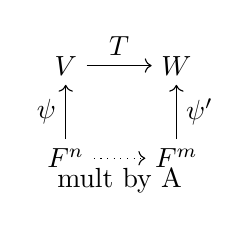
\begin{tikzpicture}[every node/.style={midway}]
                  \matrix[column sep={4em,between origins}, row sep={2em}] at (0,0) {
                              \node(V) {$V$}; & \node(W) {$W$}; \\
                                  \node(n) {$F^n$}; & \node (m) {$F^m$};\\
                                    };
                                      \draw[->] (V) -- (W) node[anchor=south]  {$T$};
                                        \draw[->] (n) -- (V) node[anchor=east] {$\psi$};
                                            \draw[dotted,->] (n) -- (m) node[anchor=north] {mult by A};
                                              \draw[->] (m) -- (W) node[anchor=west] {$\psi'$};   
        \end{tikzpicture},
        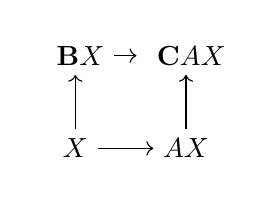
\begin{tikzpicture}[every node/.style={midway}]
                  \matrix[column sep={4em,between origins}, row sep={2em}] at (0,0) {
                          \node(V) {$\B{B}X$}; & \node(W) {$\B{C}AX$}; \\
                                  \node(n) {$X$}; & \node (m) {$AX$};\\
                                    };
                                      \draw[->] (V) -- (W) node[anchor=south]  {};
                                        \draw[->] (n) -- (V) node[anchor=east] {};
                                            \draw[->] (n) -- (m) node[anchor=north] {};
                                              \draw[->] (m) -- (W) node[anchor=west] {};   
        \end{tikzpicture}
\end{equation}

\begin{rmk}
        We say that these diagrams commute, so $T \circ \phi = \phi' \circ A$.
\end{rmk}

\vspace{15pt}

\begin{defn}[Changing Bases]
        Let $B' = (v_1',...,v_n')$ and $C' = (w_1',...,w_m')$ be new bases of $V$ and $W$. We can relate the new bases to the old one's using a matrices $P \in GL_n(F)$ and $Q \in GL_m(F)$ by $PX = X'$ and $QY = Y'$, where the non-primed letters are coordinate vectors in the old bases. Let $A'$ be the matrix of $T$ with respect to these new bases. $A'X' = Y'$, and $QAP^{-1}X' = QAX = QY = Y'$, so $A' = QAP^{-1}$.
\end{defn}




\vspace{15pt}


\begin{prop}
        Let A be a matrix of a linear transformation T with respect to some given bases $B$ and $C$. The matrices $A'$ which represents T with respect to other bases are of the form \begin{equation}
                A' = QAP^{-1}
        \end{equation}
        where $Q \in GL_m(F)$ and $P \in GL_n(F)$ are arbitrary invertible matrices. Given any $m\times n$ matrix A, there exist matrices $Q \in GL_m(F)$ and $P \in GL_n(F)$ so that $QAP^{-1}$ has the form \begin{equation}
                \left[\begin{array}{c|c} I_r & \B{0} \\ \hline \B{0} & \B{0} \end{array}\right]
        \end{equation}
\end{prop}


\vspace{15pt}




\subsection{Bases and Linear Operators}


\subsubsection{Textbook}

\begin{defn}[Linear Operator]
        A linear transformation $T: V\rightarrow V$ is called a \b{linear operator} on $V$.
\end{defn}

\vspace{15pt}

\begin{rmk}
        For linear operators we want to find a matrix when we pick only one basis $B = (v_1,...,v_n)$ fo $V$. We then write \begin{equation}
                T(B) = BA
        \end{equation}
        or \begin{equation}
                T(v_j) = \sum\limits_{i=1}^nv_ia_{ij}
        \end{equation}
        This defines the matrix $A = (a_{ij})$. In other words, $A$ is a square matrix whose jth column is the coordinate vector of $T(v_j)$ with respect to the basis $B$. If $X$ and $Y$ denote the coordinate vectors of $v$ and $T(v)$ respectively, then $Y = AX$.
\end{rmk}

\vspace{15pt}

\begin{prop}[Changing Bases]
        Suppose we have a new basis $B' = (v_1',...,v_n')$. Then if A is the matrix of the linear operator $T$ with respect to the basis $B$, and $A'$ is the matrix which represents $T$ in the new basis $B'$, then \begin{equation}
                A' = PAP^{-1}
        \end{equation}
        for some $P \in GL_n(F)$.
\end{prop}

\vspace{15pt}

\begin{defn}[Invariant Subspace]
        Let $T:V\rightarrow V$ be a linear operator on a vector space. A subspace $W$ of $V$ is called an \B{invariant subspace} or a \B{T-invariant subspace} if it is carried to itself by the operator: \begin{equation}
                TW \subset W
        \end{equation}
        In other words, $W$ is T-invariant if $T(w) \in W$ for all $w \in W$. When this is so, $T$ defines a linear operator on $W$ called the \B{restriction} of $T$ to $W$.
\end{defn}


\vspace{15pt}

\begin{cor}
        Let $T:V\rightarrow V$ be a linear operator and let $W$ be an invariant subspace. Then, let $(w_1,...,w_k)$ be a basis for $W$. We extend it to a basis $B = (w_1,...,w_k,v_1,...,v_{n-k})$ of $V$. Then, the fact that $W$ is invariant can be read off from the matrix $M$ representing $T$ with respect to the basis $B$ by the fact that the columns of the matrix are the coordinate vectors of the images of the basis vectors, and since $T(w_j)$ is in $W$, it's a linear combination of $(w_1,...,w_k)$. It follows that $M$ as a block matrix is \begin{equation}
                M = \begin{bmatrix} A & B \\ 0 & D\end{bmatrix}
        \end{equation}
        where $A$ is a $k\times k$ matrix. Moreover, $A$ is the matrix of the restriction of $T$ to $W$ with respect to the basis $(w_1,...,w_k)$.
\end{cor}

\vspace{15pt}

\begin{prop}
        Suppose that $V = W_1 \oplus W_2$ is the direct sum of two T-invariant subspaces, and $B_i$ is a basis of $W_i$. Then we can make a basis $B$ of $V$ by adjoining the bases $B_1$ and $B_2$. In this case, the matrix of $T$ with respect to $B$ will be in block diagonal form \begin{equation}
                M = \begin{bmatrix} A_1 & 0 \\ 0 & A_2 \end{bmatrix}
        \end{equation}
        Where $A_i$ is the matrix of $T$ restricted to $W_i$.
\end{prop}


\vspace{15pt}

\begin{defn}[Eigenvectors]
        An \B{eigenvector} $v$ for a linear operator $T$ is a nonzero vector such that \begin{equation}
                T(v) = cv
        \end{equation}
        for some scalar $c \in F$. Here $c$ is called the \B{eigenvalue} associated to the eigenvector $v$.
\end{defn}

\vspace{15pt}

\begin{cor}
        Let $v$ be an eigenvector for a linear operator $T$. Then the subspace $W$ spanned by $v$ is T-invariant, because $T(av) = acv \in W$ for all $a \in F$. Conversely, if this subspace is invariant, then $v$ is an eigenvector. Thus, an eigenvector is a basis of a T-invariant one-dimensional subspace.
\end{cor}

\vspace{15pt}

\begin{cor}
        Similar or conjugate matrices have the same eigenvalues.
\end{cor}

\vspace{15pt}


\begin{prop}
        The basis vector $v_j$ is an eigenvector of $T$, with eigenvalue $c$, if and only if the jth column of A has the form $ce_j$, for the matrix $A$ is defined by the property $T(v_j) = v_1a_{1j}+...+v_na_{nj}$, so if $T(v_j) = cv_j$ then $a_{jj} = c$ and $a_{ij} = 0$ for $i \neq j$.
\end{prop}


\vspace{15pt}



\begin{cor}
        With the above notation, the matrix $A$ of a linear operator $T$ with respect to a basis $B$ is diagonal if and only if $B$ is a basis of eigenvectors of $T$.
\end{cor}

\vspace{15pt}

\begin{cor}
        The matrix A of a linear transformation is similar or conjugate to a diagonal matrix if and only if there is a basis $B' = (v_1',...,v_n')$ of $V$ made up of eigenvectors.
\end{cor}

\vspace{15pt}

\begin{lem}
        The following conditions on a linear operator $T:V\rightarrow V$ on a finite dimensional vector are equivalent: \begin{enumerate}
                \item $\nullity(T) > 0$
                \item $\rank(T) < \dim(V)$
                \item If A is the matrix of the operator with respect to an arbitrary basis, then $\det(A) = 0$
                \item $0$ is an eigenvalue of $T$
        \end{enumerate}
\end{lem}

\vspace{15pt}

\begin{defn}[Singular and Non-Singular]
        A linear operator $T$ on a finite-dimensional vector space $V$ is called \B{singular} if it satisfies any of the equivalent conditions in the above lemma. Otherwise, $T$ is \B{nonsingular}
\end{defn}

\vspace{15pt}

\begin{prop}
        The operator $T$ has an eigenvalue $c$ if and only if the operator $T - cI$ has a non-zero kernel.
\end{prop}


\vspace{15pt}

\begin{cor}
        The eigenvalues of a linear operator $T$ are scalars $c \in F$ such that $T - cI$ is singular.
\end{cor}


\vspace{15pt}

\begin{defn}[Characteristic Polynomial]
        The \B{characteristic polynomial} of a linear operator $T$ is the polynomial \begin{equation}
                p(t) = \det(tI - A)
        \end{equation}
        where $A$ is the matrix of $T$ with respect to some basis. Then, $c \in F$ is an eigenvalue if and only if $p(c) = 0$.
\end{defn}


\vspace{15pt}

\begin{cor}
        The eigenvalues of a linear operator are the roots of its characteristic polynomial.
\end{cor}

\vspace{15pt}

\begin{cor}
        The eigenvalues of an upper or lower triangular matrix are its diagonal entries.
\end{cor}

\vspace{15pt}

\begin{prop}
        The characteristic polynomial of an operator $T$ does not depend on the choice of basis.
\end{prop}

\vspace{15pt}

\begin{prop}
        The characteristic polynomial $p(t)$ has the form \begin{equation}
                p(t) = t^n - (\tr A)t^{n-1} + (intermediate\;terms)+ (-1)^n(\det A)
        \end{equation}
\end{prop}

\vspace{15pt}

\begin{prop}
        Let $T$ be a linear operator on a finite-dimensional vector space $V$.\begin{enumerate}
                \item If $V$ has dimension $n$, then $T$ has at most $n$ eigenvalues.
                \item If $F$ is a field of complex numbers and $V \neq \{0\}$, then $T$ has at least one eigenvalue, and hence it has an eigenvector.
        \end{enumerate}
\end{prop}

\vspace{15pt}




\subsubsection{Lecture}


Let $V$ and $W$ be finite dimensional vector spaces over the field $F$. Let $T:V\rightarrow W$ is a linear transformation.

\begin{eg}
        Let $V = F[x]_{deg\leq n}$ and $W = F[x]_{deg\leq n -1}$, then $T:\frac{d}{dx}:V\rightarrow W$ is a linear operator. Moreover, the \B{total derivative of a function} $f:\R^n \rightarrow \R^m$ is a linear map. What is $\ker\left(\frac{d}{dx}\right)$ when $F = \Z/p\Z$? Well, $F \subset \ker(T)$. But, if $n \geq p$, we also have $x^p$ in the kernel, since \begin{equation}
                \frac{d}{dx}(x^p) = px^{p-1} = 0
        \end{equation}
\end{eg}

\vspace{15pt}

\begin{defn}[Kernel and Image]
        We define \begin{equation}
                \ker(T) := \{v \in V: T(v) = 0\} \subset V
        \end{equation}
        and \begin{equation}
                \im(T) := \{w \in W: w = T(v)\} \subset W
        \end{equation}
\end{defn}

\vspace{15pt}

\begin{thm}[Dimension Formula]
        \begin{equation}
                \dim(V) = \dim(\ker(T)) + \dim(\im(T))
        \end{equation}
\end{thm}
\begin{proof}
        Let $\{v_1,...,v_k\}$ be a basis of $\ker(T)$. Then since it is linearly independent, we can extend it to a basis $\{v_1,...,v_k,v_{k+1},...,v_n\}$ of $V$. Then, let $w_i = T(v_{k+i})$ for all $i = 1,...,n-k$. Note that the set $\{w_1,...,w_{n-k}\}$ spans $\im(T)$ since \begin{equation}
                w = T(v) = T\left(\sum\limits_{i=1}^ka_iv_i+\sum\limits_{k+1}^nb_iv_i\right) = \sum\limits_{i=1}^ka_iT(v_i)+\sum\limits_{k+1}^nb_iT(v_i) = \sum\limits_{k+1}^nb_iw_i
        \end{equation}
        for any $w \in \im(T)$. Now, suppose we have a linear relation $\sum b_iw_i = 0_W$. Consider the vector $v_0 = \sum_{i=1}^{n-k} b_i v_{i+k}$ in $V$. Then by our linear relation, $T(v_0) = 0_W$. Therefore, by definition $v_0 \in \ker(T)$, so we can express it as $v_0 = \sum_{i=1}^{k}a_iv_i = \sum_{i=1}^{n-k}b_iv_{i+k}$. This give the linear relation \begin{equation}
                \sum_{i=1}^{k}a_iv_i - \sum_{i=1}^{n-k}b_iv_{i+k} = 0_V
        \end{equation}
        This is a linear relation on a basis of $V$, so all $a_i = 0$ and $b_i = 0$. Therefore, the set $\{w_1,...,w_{n-k}\}$ is linearly independent. Thus $\{w_1,...,w_{n-k}\}$ is a basis, and the proof is complete.
\end{proof}

\vspace{15pt}

\begin{cor}
        If $V$ is finite-dimensional and $W \subset V$ is a subspace, then $\dim(W) + \dim(V/W) = \dim(V)$
\end{cor}
\begin{proof}
        There exists a canonical homomorphism $T: V\rightarrow V/W$, $v \mapsto v+W$, which is surjective with kernel $W$.
\end{proof}

\vspace{15pt}

\begin{nota}
        The dimension of the image is also known as the \B{rank} of $T$, and the dimension of the kernel is known as the \B{nullity} of $T$.
\end{nota}

\vspace{15pt}


\begin{defn}[Linear Operators and Bases]
        Let $\{v_1,...,v_n\}$ be a basis of $V$ and $\{w_1,...,w_m\}$ be a basis of $W$. Then the basis of $V$ corresponds to a lienar isomorphism $V \rightarrow F^n$ which takes any $v = \sum\limits_{i=1}^na_iv_i \mapsto [a_1 ... a_n]^T$. (A choice of a basis gives you an isomorphism between any abstract space to the canonical vector space of the same dimension). A similarly isomorphism arises for the basis of $W$.
\end{defn}

\vspace{15pt}

\begin{qst}
        What does $T:V\rightarrow W$ look like once these isomorphisms have been chosen?
\end{qst}

\begin{figure}[H]
        \centering
        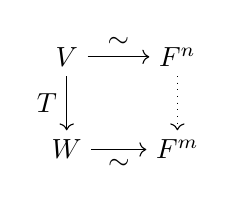
\begin{tikzpicture}[every node/.style={midway}]
                  \matrix[column sep={4em,between origins}, row sep={2em}] at (0,0) {
                              \node(V) {$V$}  ; & \node(n) {$F^n$}; \\
                                  \node(W) {$W$}; & \node (m) {$F^m$};\\
                                    };
                                      \draw[<-] (W) -- (V) node[anchor=east]  {$T$};
                                        \draw[->] (V) -- (n) node[anchor=south] {$\sim$};
                                            \draw[dotted,->] (n) -- (m) node[anchor=west] {};
                                              \draw[->] (W) -- (m) node[anchor=north] {$\sim$};
        \end{tikzpicture}
\end{figure}
\begin{ans}
        Each $T(v_j) = \sum\limits_{i=1}^m a_{ij}w_i$ for $j = 1,2,...,n$, where $a_{ij} \in F$ are determined by $T$ and the choice of bases (By the fact that the $w_i$ form a basis of $W$). Conversely, the scalars $\{a_{ij}\}_{i=1,j=1}^{i=m,j=n}$ determine $T$ uniquely. Why? Because we write $v = \sum\limits_{j=1}^nx_jv_j$, so \begin{equation}
                T(v) = \sum\limits_{j=1}^nx_j\left(\sum\limits_{i=1}^ma_{ij}w_i\right)
        \end{equation}
        If we define $A$ to be the $m\times n$ matrix $(a_{ij})$, which means we put the coordinate of the image of $v_j$ in the jth column \begin{equation}
                A = \begin{bmatrix}  & & \Big\vert & & \\ \hdots & \hdots & [T(v_j)]_W & \hdots & \hdots \\ & & \Big\vert & & \end{bmatrix}
        \end{equation}
        Then, if we write $T(v) = \sum\limits_{i=1}^my_iw_i$, with $y_i = \sum\limits_{j=1}^n a_{ij}x_j$ really is the formula \begin{equation}
                \begin{bmatrix} y_1 \\ \vdots \\ y_m \end{bmatrix} = Y = AX = A\begin{bmatrix} x_1 \\ \vdots \\ x_n \end{bmatrix}
        \end{equation}
        Therefore, associated to a linear transformation and the choices of bases for the domain and codomain is a set of $mn$ scalars which we put in a matrix, and the linear transformation is given by left multiplying the vector by $A$.
\end{ans}

\begin{figure}[H]
        \centering
        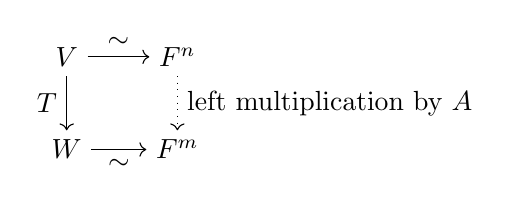
\begin{tikzpicture}[every node/.style={midway}]
                  \matrix[column sep={4em,between origins}, row sep={2em}] at (0,0) {
                              \node(V) {$V$}  ; & \node(n) {$F^n$}; \\
                                  \node(W) {$W$}; & \node (m) {$F^m$};\\
                                    };
                                      \draw[<-] (W) -- (V) node[anchor=east]  {$T$};
                                        \draw[->] (V) -- (n) node[anchor=south] {$\sim$};
                                            \draw[dotted,->] (n) -- (m) node[anchor=west] {left multiplication by $A$};
                                              \draw[->] (W) -- (m) node[anchor=north] {$\sim$};
        \end{tikzpicture}
\end{figure}


\vspace{15pt}

\begin{eg}
        Take $T: V \rightarrow W$ with $V$ with a basis $\{v_1,v_2\}$ and $W$ has a basis $\{w_1,w_2\}$, and $T(v_1) = 2w_1$ and $T(v_2) = 3w_1+4w_2$. Then the matrix is \begin{equation}
                A = \begin{bmatrix} 2 & 3 \\ 0 & 4 \end{bmatrix}
        \end{equation}
        Let $v = 7v_1 + 8v_2$. Then \begin{equation}
                [T(v)] = A[7 \; 8 ]^T = [38 \; 32]^T
        \end{equation}
        Which implies that $T(v) = 38w_1+32w_2$.
\end{eg}

\vspace{15pt}


\begin{rmk}[Special Case]
        If we have a linear transformation $T:V\rightarrow V$ (an \B{endomorphism} - a homomorphism from a vector space to itself) and consider one basis $B= \{v_1,...,v_n\}$, then we get a square matrix $A = [T]_B$. Moreover, if we have another endomorphism $S:V\rightarrow V$, and $S$ has matrix $B$ (n by n), then the matrix for $S\circ T:V\rightarrow V$ is $B\cdot A$ given by matrix multiplication (this is how matrix multiplication is derived as the composition of linear operators). 
\end{rmk}

\vspace{15pt}

\begin{prop}
        For a transformation $T:V\rightarrow V$, the following are equivalent:
        \begin{enumerate}
                \item T is an automorphism of vector spaces
                \item $\ker(T) = \{0_V\}$
                \item $\im(T) = V$
                \item If the matrix A of $T$, with respect to $\{v_1,...,v_n\}$ is A, then A is invertible 
                \item $\det(A) \neq 0$ in $F$.
        \end{enumerate}
\end{prop}


\vspace{15pt}

\begin{defn}
        The set of all $T:V\rightarrow V$ which are isomorphisms forms a group $GL(V)$, and is isomorphic to $GL_n(F)$, where $\dim(V) = n$. So really, $GL_n(F)$ can be thought of as invertible linear transformations of an n-dimensional vector space over the field $F$.
\end{defn}


\vspace{15pt}

\begin{eg}
        Let $F = \Z/2$. What is the group $GL_2(F)$. Note we have 16 choices of $2\times 2$ matrices over $F$, but only six of them are invertible. Moreover, $GL_2(F) \cong S_3$.
\end{eg}


\vspace{15pt}

\begin{defn}[Change of Basis]
        If A is the matrix of a transformation $T: V\rightarrow V$ with respect to the basis $B = \{v_1,...,v_n\}$, what is the matrix with respect to the basis $B' = \{v_1',...,v_n'\}$ $A'$? Then $A' = PAP^{-1}$, where $P$ is the invertable $n\times n$ matrix giving the change of basis.  $A'$ is also called the conjugate matrix.
\end{defn}

\vspace{15pt}

\begin{rmk}
        The advantage of the $(V,T)$ point of view over the $(F^n,A)$ point of view is by choosing a convenient basis, we can get a simpler form for our operator.
\end{rmk}

\vspace{15pt}

\begin{eg}[Two Bases]
        From our first proposition: $T:V\rightarrow W$. \\
        There exists a basis of $V$ and a basis of $W$ so that the matrix of $T$ is \begin{equation}
                \begin{bmatrix} \begin{bmatrix} 1_1 & & & 0 & \\ & 1_2 & & & \\ & & \ddots & & \\ 0 & & & 1_{r-1} & \\ & & & & 1_r  \end{bmatrix} & \B{0} \\ \B{0} & \B{0} \end{bmatrix}
        \end{equation}
        where $r = rank(T)$. We take basis $\{v_{k+1},...,v_{n},v_1,...,v_k\}$ where the first part maps to the basis of the image, the second part maps to the kernel, and for $W$ we take $\{T(v_{k+1}),...,T(v_{n}),......\}$.
\end{eg}

\vspace{15pt}

\begin{eg}[One Basis]
        A more interesting case is for $T: V\rightarrow V$. \\
        We seek to find a basis of \B{eigenvectors} so that $T(v) = cv$. If we found a basis of such, then we find the matrix \begin{equation}
                A = \begin{bmatrix} c_1 & & & 0 \\ & c_2 & & \\ & & \ddots & \\ 0 & & & c_n \end{bmatrix}
        \end{equation}
\end{eg}

\vspace{15pt}

\begin{qst}
        Let $T:V\rightarrow V$ be a linear operator. Can we fina good basis so that the matrix A of $T$ is in simple form?
\end{qst}

\vspace{15pt}

\begin{defn}[T-Invariant]
        An \B{invariant subspace} $W \subset V$ is a subspace such that $T(W) \subset W$. If you make a matrix A of $T$ with respect to a basis extended from a basis of $W$, then \begin{equation}
                A = \left[\begin{array}{c|c} a & b \\ 0 & d \end{array}\right]
        \end{equation}
        so the first basis vectors are in $W$, and so are the $T(w_i)$.
\end{defn}

\vspace{15pt}

\begin{defn}[Invariant Complement]
        Suppose $W$ is a T-invariant subspace of $V$, and it has an \B{invariant complement} $W'$, which implies each element of $V$ can be denoted uniquely by the sum of a vector in $W$ and a vector in $W'$, and we denote it by the \B{direct sum} $V = W\oplus W'$. Then, the matrix $A$ of the transformation with respect to a basis of $V$ obtained from adjoining a basis of $W$ to a basis of $W'$ has the form \begin{equation}
                A = \left[\begin{array}{c|c} a & 0 \\ 0 & d \end{array}\right]
        \end{equation}
\end{defn}

\vspace{15pt}

\begin{rmk}
        An extreme case of this is if $W$ is one dimensional, $W = Fw:= \{cw: c\in F\}$, and is invariant, then $Tw = cw$. We then say that $w$ is an eigenvector of $T$ with associated eigenvector $c$. If there is a basis $\{v_1,...,v_n\}$ of $V$ consisting of eigenvectors with eigenvalues $c_1,..,c_n$, then the associated matrix for T is \begin{equation}
                A = \begin{bmatrix} c_1 & & & 0 \\ & c_2 & & \\ & & \ddots & \\ 0 & & & c_n \end{bmatrix}
        \end{equation}
        The eigenbasis gives a decomposition of the space into lines (one-dimensional vector spaces), each stable under $T$, such that $V$ is the direct sum of those lines, and the matrix of $T$ can be represented very simply.
\end{rmk}


\vspace{15pt}

\begin{eg}[Counter-Example]
        .\newline \begin{enumerate}
                \item Consider the rotation of $\R^2$ by an angle $\theta$. In the standard basis, the matrix representation of the rotation is \begin{equation} 
                                A = \begin{bmatrix} \cos(\theta) & -\sin(\theta) \\ \sin(\theta) & \cos(\theta) 
                        \end{bmatrix}
                \end{equation}
                \item Here, the transformation has no eigenvectors. Consider the linear operator $T: F^2 \rightarrow F^2$ so that $T(e_1) = e_1$ and $T(e_2) = e_1 + e_2$, so it has a matrix over the standard basis of the form \begin{equation} 
                                A = \begin{bmatrix} 1 & 1 \\ 0 & 1 \end{bmatrix}
                \end{equation}
                        There is no basis of eigenvectors (There is no complement $W'$ which is T-invariant where $W = Fe_1$).
        \end{enumerate}
\end{eg}

\vspace{15pt}

\begin{qst}
        Given $T$, what are the possible eigenvalues?
\end{qst}
\begin{ans}
        If $Tw = cw$, and you consider the new operator $(T-cI)$, then $(T-cI)w = 0$. In other words, $w$ is in the kernel of the linear operator $T-cI$. So, $T-cI$ is not invertible since it has a non-trivial kernel. Conversely, if $T-cI$ has a kernel (or just is not invertible) then $c$ is an eigenvalue for $T$.
\end{ans}

\vspace{15pt}

\begin{rmk}
        The set of eigenvalues is equal to the set of $c \in F$ such that $T-cI$ is not invertible. This is equivalent to $\det(A - cI) = 0$, where $A$ is the matrix of $T$ with respect to some basis.
\end{rmk}


\vspace{15pt}

\begin{defn}[Characteristic Polynomial]
        Consider the determinant $\det(tI - A)$, where \begin{equation}
                tI - A = \begin{bmatrix} t - a_{11} & -a_{12} & \hdots & -a_{1n} \\ -a_{21} & t-a_{22} & & \vdots\\ \vdots & & \ddots & \\ -a_{n1} & \hdots & & t-a_{nn} \end{bmatrix}
        \end{equation}
        Then $\det(tI - A) = t^n - (a_{11}+a_{22}+...+a_{nn})t^{n-1} + ... + (-1)^n\det A = p(t)$ is a polynomial in $t$ of degree $n$ with coefficients in the field $F$. This is the \B{characteristic polynomial of T}, where its roots $c$ are the eigenvalues of $T$.
\end{defn}

\vspace{15pt}

\begin{obs}
        Tbe characteristic polynomial $p(t)$ depends only on $T$, not on the basis of $V$ used to obtain the matrix $A$ to calculate it. If we used a different basis, then we get $A' = PAP^{-1}$. Observe that \begin{equation}
                \det(tI - A')=\det(tI - PAP^{-1}) = \det(P(tI - A)P^{-1}) = \det(P)p(t)\det(P^{-1}) = p(t)
        \end{equation}
\end{obs}

\vspace{15pt}

\begin{lem}
        If $p(t)$ has degree $n$ over a field $F$, then it has at most $n$ distinct roots $c$ in $F$.
\end{lem}
\begin{proof}
        By the Euclidean Algorithm for polynomials, $f(t) = (t-c)g(t) + d$ with $\deg g(t) = n-1$, $d \in F$. If $f(c) = 0$, then $d = 0$, so $f(t) = (t-c)g(t)$. If $c'$ is another root with $c' \neq c$, then $g(c') = 0$. Then, we use induction on the degree of $g$.
\end{proof}

\vspace{15pt}

\begin{cor}
        The roots of the characteristic polynomial are eigenvalues, so we have at most $n$ distinct eigenvalues, where $n = \dim(V)$.
\end{cor}

\vspace{15pt}

\begin{eg}
        Let $A = \begin{bmatrix} a& b \\ c & d\end{bmatrix}$, then $p(t) = t^2 - (a+d)t + (ad - bc)$.
\end{eg}


\vspace{15pt}

\begin{eg}
        Let $A = \begin{bmatrix} 3& 2 \\ 1 & 4\end{bmatrix}$, then $p(t) = t^2 - 7t + 10$, so it has eigenvalues $2$ and $5$. Then if $2 \neq 5$ in $F$, then we obtain a basis of eigenvectors.
\end{eg}


\vspace{15pt}

\begin{cor}
        If your characteristic polynomial factors as $p(t) = (t-c_1)(t-c_2)...(t-c_n)$ with $c_i \neq c_j$, $i \neq j$, then you have a basis of eigenvectors for your linear operator.
\end{cor}


\vspace{15pt}


\begin{rmk}
        Take a linear operator $T:V\rightarrow V$ on a finite-dimensional vector space, then it gives a vector in $Hom(V,V)$ (a vector space of all linear maps over $V$, where if $\dim(V) = n$, then $\dim(Hom(V,V)) = n^2$). Consider $\{I,T,T^2,...,T^{n^2}\}$. Since there are $n^2+1$ of them, they must be linearly dependent. Thus, there must be a linear relation \begin{equation}
                a_0I + a_1T+a_2T^2+...+a_{n^2}T^{n^2} = 0
        \end{equation}
        in $Hom(V,V)$, where $0$ is the zero operator. In other words $T$ satisfies a polynomial of degree $\leq n^2$ with coefficients in $F$. If we let $F(t) = a_0 + a_1t + ... + a_{n^2}t^{n^2}$, then $F(T) = 0$.
\end{rmk}

\begin{thm}[Caley-Hamilton Theorem]
        $T$ always satisfies its own characteristic polynomial (a polynomial of degree $n$).
\end{thm}

\begin{proof}
        When $f(t) = (t-c_1)(t-c_2)...(t-c_n)$, where all $c_i$ are distint. Then we can find a matrix representation of $T$ with the eigenvalues along the diagonal, and all other entries zero. Then, $f(A) = (A-c_1I)(A-c_2I)...(A-c_nI) = 0$ since each matrix binomial will have its ith row will be zero, where $i$ corresponds to the $c_i$ of the binomial.
\end{proof}


\vspace{15pt}

\begin{eg}
        Let $A = \begin{bmatrix} a& b \\ c & d\end{bmatrix}$, then $p(t) = t^2 - (a+d)t + (ad - bc)$. Then $A^2 = \begin{bmatrix} a^2+bc & ab+bd \\ ac+dc & bc+d^2 \end{bmatrix}$. Plugging $A^2$ into the characteristic polynomial we obtain \begin{equation}
                p(A) = \begin{bmatrix} 0 & 0 \\ 0 & 0 \end{bmatrix}
\end{equation}
\end{eg}


\subsection{Orthogonal Matrices and Groups}

\subsubsection{Textbook}

\begin{rmk}
        In $\R^3$, a rotation about the origin can be described by a pair $(v,\theta)$ consisting of a unit vector $v$, which lies in the axis of rotation, and a nonzero angle $\theta$.
\end{rmk}


\vspace{15pt}

\begin{defn}[Orthogonal Matrix]
        A real $n\times n$ matrix $A$ is said to be orthogonal if $A^T = A^{-1}$, or equivalently if $A^TA = I$. The orthogonal $n\times n$ matrices form a subgroup of $GL_n(\R)$ denoted by $O_n$ and called the orthogonal group: \begin{equation}
                O_n := \{A \in GL_n(\R): A^TA = I\}
        \end{equation}
        The determinant of an orthogonal matrix is $\pm 1$ since $A^TA = I$ implies that \begin{equation}
                (\det(A))^2 = \det(A)\det(A^T) = 1
        \end{equation}
\end{defn}

\vspace{15pt}

\begin{rmk}
        The orthogonal matrices having determinant $+1$ form a subgroup called the \B{special linear orthogonal group}, and denoted \begin{equation}
                SO_n :=\{A \in GL_n(\R): A^TA= I, \det(A) = 1\}
        \end{equation}
        This subgroup has one coset in addition to $SO_n$, which is the set of elements with determinant $-1$. Thus, $[O_n:SO_n] = 2$.
\end{rmk}

\vspace{15pt}

\begin{thm}
        The rotations of $\R^2$ and $\R^3$ about the origin are the linear operators whose matrices with respect to the standard basis are orthogonal and have determinant $1$. In other words, a matrix A represents a rotation of $\R^2$ (or $\R^3$) if and only if $A \in SO_2(\R)$ (or $SO_3(\R)$).
\end{thm}

\vspace{15pt}

\begin{cor}
        The composition of two rotations about the origin in $\R^3$ is also a rotation.
\end{cor}

\vspace{15pt}

\begin{defn}[Dot Product]
        The dot product of real column vectors $X$ and $Y$ is $(X\cdot Y) = x_1y_1 + ... + x_ny_n = X^TY$. Over the reals, the dot product is the square of the norm of a vector, $x\cdot x = ||x||^2$, and $(X\cdot Y) = ||X||||Y||\cos(\theta)$, where $\theta$ is the angle between the vectors $X$ and $Y$ (consequence of the law of cosines).
\end{defn}

\vspace{15pt}

\begin{defn}[Orthogonality]
        Two vectors $X$ and $Y$ are orthogonal if and only if $(X\cdot Y) = 0$.
\end{defn}

\vspace{15pt}

\begin{prop}
        The following conditions on a real $n\times n$ matrix $A$ are equivalent: \begin{enumerate}
                \item $A$ is orthogonal
                \item Multiplication by $A$ preserves the dot product, that is, $(AX\cdot AY) = (X\cdot Y)$ for all column vectors $X$ and $Y$.
                \item The columns of $A$ are mutually orthogonal unit vectors. That is, they form an orthonormal basis for $\R^n$
        \end{enumerate}
\end{prop}
\begin{proof}
        If $A$ is orthogonal, then $(AX\cdot AY) = (AX)^TAY = X^TA^TAY = X^TY = (X\cdot Y)$. Conversely, suppose $X^TY = X^TA^TAY$ for all $X$ and $Y$. Let $B = I - A^TA$, so $X^TBY = 0$. Note that for any $B$, $e_i^TBe_j = b_{ij}$, so if $X^TBY = 0$ for all $X$ and $Y$, then $b_{ij} = 0$ for all $i=1,...,n$ and $j = 1,...,n$. Thus, $B=0$ and $I = A^TA$. Let $A_j$ denote the jth column vector of A. The $(i,j)$ entry of the product matrix $A^TA$ is $(A_i \cdot A_j)$. Thus, $A^TA = I$ if and only if $(A_i\cdot A_i) = 1$ for all $i$, and $(A_i \cdot A_j) = 0$ for all $j \neq i$. Thus the columns of $A$ have length 1 and are orthogonal, proving the equivalence of (1) and (3).
\end{proof}



\vspace{15pt}


\begin{defn}[Rigid Motion or Isometry]
        A \B{rigid motion} or \B{isometry} of $\R^n$ is a map $m:\R^n\rightarrow \R^n$ which preserves distances; that is, if $X$ and $Y$ are in $\R^n$, then the distance from $X$ to $Y$ is equal to the distance from $m(X)$ to $m(Y)$ \begin{equation}
                |m(X) - m(Y)| = |X - Y|
        \end{equation}
        Such motions preserve angles and shapes in general. Moreover, the rigid motions of $\R^n$ form a group $M_n$, with composition of operations as its law of composition, and it is often called \B{the group of motions}.
\end{defn}

\vspace{15pt}

\begin{prop}
        For a map $m:\R^n \rightarrow \R^n$, the following conditions are equivalent: \begin{enumerate}
                \item m is a rigid motion which fixes the origin
                \item m preserves the dot product: that is, for all $X,Y \in \R^n$, $(m(X)\cdot m(Y)) = (X\cdot Y)$
                \item m is left multiplication by an orthogonal matrix
        \end{enumerate}
\end{prop}
\begin{proof}
        Suppose m is a rigid motion which fixes $0$. The fact that m preserves distances means \begin{equation}
                (m(X)-m(Y)\cdot m(X) - m(Y)) = (X - Y \cdot X - Y)
        \end{equation}
        for all vectors $X$ and $Y$. Setting $Y =0$ shows that $(m(X)\cdot m(X)) = (X \cdot X)$. Expanding both sides and cancelling terms gives $(m(X)\cdot m(Y)) = (X\cdot Y)$. This shows that m preserves the dot product, so (1) implies (2).

        Next, suppose m preserves the dot product. First, note that if $m$ fixed the basis vectors $e_i$ then it is the identity as \begin{equation*}
                x_j = (X\cdot e_j) = (m(X) \cdot m(e_j)) = (m(X) \cdot e_j) = m(x)_j
        \end{equation*}
        for all $j$. Hence, $X = m(X)$, and $m$ is the identity. 

        Now, since $m$ preserves the dot product, the images $m(e_1),...,m(e_n)$ of the standard basis vectors are orthogonal: $(m(e_i)\cdot m(e_i)) = (e_i\cdot e_i) = 1$ and $(m(e_i)\cdot m(e_j)) = (e_i \cdot e_j) = 0$, for $i \neq j$. Let $B' = (m(e_1),...,m(e_n))$ and $A = [B']$. Then the columns of $A$ form an orthonormal basis of $\R^n$ by definition, so $A$ is orthogonal. Note that $A^{-1} = A^T$ is also orthogonal, so multiplication by $A^{-1}$ preserves the dot-product. Moreover, the composed motion $A^{-1}m$ preserves the dot product and fixes the basis vectors $e_i$. Thus, $A^{-1}m$ is the identity map. This shows m is left multiplication by $A$ as required.

        Finally, if m is a linear operator whose matrix, $A$, is orthogonal, then $m(X) - m(Y) = m(X-Y)$ because m is linear, and $||m(X) - m(Y)|| = ||m(X-Y)|| = ||X - Y||$ by the fact that orthogonal matrices preserve dot products. Thus, m is a rigid motion. Since a linear operator always fixes $0$, we see that (3) implies (1).
\end{proof}



\vspace{15pt}

\begin{cor}
        A rigid motion witch fixes the origin is a linear operator.
\end{cor}

\vspace{15pt}


\begin{defn}[Translation]
        A \B{translation} is a rigid motion $t_b$ of the form \begin{equation}
                t_b(X) = X + b = \begin{bmatrix} x_1 + b_1 \\ \vdots \\ x_n + b_n \end{bmatrix}
        \end{equation}
        where $b$ is some fixed vector in $\R^n$.
\end{defn}

\vspace{15pt}

\begin{prop}
        Every rigid motion m is the composition of an orthogonal linear operator and a translation. In other words, it has the form $m(X) = AX + b$ for some orthogonal matrix $A$ and fixed vector $b$.
\end{prop}
\begin{proof}
        Let $b = m(0)$. Then $t_{-b}(b) = 0$, so the composed operation $t_{-b}m$ is a rigid motion which fixes the origin. Then, $t_{-b}m$ is realized by left multiplication by a orthogonal matrix $A$, so $t_{-b}m(X) = AX$. Applying $t_b$ we see that $m(X) = AX + b$. Note that both the vector $b$ and matrix $A$ are uniquely determined by $m$, because $b = m(0)$ and $A$ is the operator $t_{-b}(m)$.
\end{proof}

\vspace{15pt}

\begin{defn}
        An orthogonal operator is called \B{orientation preserving} if its determinant is $+1$, and \B{orientation reversing} if it is $-1$. Similarly, a rigid motion $m$ is \B{orientation preserving} if $\det A = 1$ and \B{orientation reversing} if $\det A = -1$.
\end{defn}

\vspace{15pt}

\begin{cor}
        The rotations of $\R^2$ and $\R^3$ are the orientation preserving rigid motions which fix the origin.
\end{cor}


\vspace{15pt}


\begin{lem}
        Every element $A \in SO_3$ has the eigenvalue $1$.
\end{lem}

\vspace{15pt}

\subsubsection{Lecture}


\begin{defn}[Orthogonal Groups]
        Suppose that $F$ is a field. Then $GL_n(F)$ is the \B{general linear group} over $F$ composed of $n\times n$ invertible matrices with coefficients in $F$. Then $O_n(F) \subset GL_n(F)$ is a subgroup called the \B{orthogonal linear group} composed of orthogonal $n\times n$ matrices with coefficients in $F$. Finally, $SO_n(F) \nsub O_n(F)$ is the \B{special orthogonal linear group} composed of orthogonal $n\times n$ matrices with coefficients in $F$ and determinant $1$.
\end{defn}


\vspace{15pt}

\begin{defn}[Orthogonal Groups]
        Take the vector space $V = F^n$, then $GL_n(F)$ is the group of linear maps on $V$ which are isomorphisms. We put additional structure on $V$, which is an \B{inner product} $\langle , \rangle: F^n\times F^n \rightarrow F$ (more generally \B{bilinear forms}) which has the properties \begin{enumerate}
                \item For $v = (a_1,...,a_n)$ and $w = (b_1,...,b_n)$, then $\langle v, w \rangle = \sum\limits_{i=1}^na_ib_i$
        \end{enumerate}
        We define \begin{equation}
                O_n(F) := \{A \in GL_n(F): \langle Av, Aw\rangle \langle v, w \rangle \}
        \end{equation}
        Certainly, $I \in O_n(F)$. Moreover, for $A,B \in O_n(F)$, $$\langle ABv, ABw\rangle = \langle A(Bv), A(Bw) \rangle = \langle Bv, Bw \rangle = \langle v, w \rangle$$ so $AB \in O_n(F)$. Finally, for $A \in O_n(F)$, \begin{equation}
                \langle A^{-1}v, A^{-1}w \rangle = \langle A(A^{-1}v), A(A^{-1}w) \rangle = \langle v, w \rangle
        \end{equation}
        Thus, $O_n(F)$ is a subgroup of $GL_n(F)$. 
\end{defn}


\vspace{15pt}


\begin{rmk}[Shape of Orthogonal Matrices]
        Note that for the standard basis of $V = F^n$, $\langle e_i, e_i \rangle = 1$ for all $i$, and $\langle e_i, e_j \rangle = 0$ for $i \neq j$. Furthermore, note that the jth column of a matrix $A \in O_n(F)$ is given by $A(e_j)$. Then since $A$ preserves the inner product, the inner product of the jth column with itself must be 1. Moreover, the inner product of the jth column with the ith column must be zero for $i \neq j$. This implies that \begin{equation}
                \langle Ae_i,Ae_j\rangle = \left\{ \begin{array}{cc} 1 & if\;i=j \\ 0 & if\; i\neq j \end{array}\right.
        \end{equation}
        Then it follows that \begin{equation}
                A^TA = I
        \end{equation}
        since the ij-th entry of $A^TA$ is the inner product of the i-th and j-th columns of $A$, which gives 1's along the diagonal, and zeroes everywhere else. This is equivalent to saying that \begin{equation}
                A^T = A^{-1}
        \end{equation}
\end{rmk}


\vspace{15pt}


\begin{prop}
        Conversely, if $A \in GL_n(F)$ has $A^T = A^{-1}$, then it preserves the inner product we have defined on the vector space $V = F^n$, and hence $A \in O_n(F)$.
\end{prop}
\begin{proof}
        First, note that if $v$ and $w$ are column vectors, $\langle v, w \rangle = v^T\cdot w$, where $\cdot$ is the matrix product. Then observe that $\langle Av, Aw \rangle = (Av)^T\cdot Aw = v^TA^TAw = v^Tw = \langle v, w \rangle$. Therefore, $A \in O_n(F)$, as $A$ preserves the inner product. 
\end{proof}

\vspace{15pt}

\begin{cor}
        Then, $O_n(F) = \{A \in GL_n(F): A^T = A^{-1}$.
\end{cor}

\vspace{15pt}

\begin{prop}
        For all $A \in O_n(F)$, $\det(A) = \pm 1$.
\end{prop}


\vspace{15pt}

\begin{defn}[Special Orthogonal Group]
        If we take the homomorphism $\det:O_n(F) \surrightarrow F$, then the kernel of the homomorphism is the \B{special linear orthogonal group} $SO_n(F) := \{A \in O_n(F): \det(A) = 1\}$, and $[O_n(F): SO_n(F)] = 2$ (if $1 \neq -1$ in $F$)
\end{defn}

\vspace{15pt}

\begin{prop}
        The permutation matrices are in $O_n(F)$, which gives an injective homomorphism $f:S_n \hookrightarrow O_n(F)$, and $A_n \nsub S_n$, then the restriction $f\;\Big\vert_{A_n}A_n\hookrightarrow SO_n(F)$. Thus, we can consider $S_n$ as a finite subgroup of the orthogonal group over ANY field.
\end{prop}
\begin{rmk}[WARNING]
        If $1 = -1$ in $F$, then the determinant homomorphism for $O_n(F)$ has only a trivial image, and $SO_n(F) = O_n(F)$.
\end{rmk}


\vspace{15pt}

\begin{rmk}
        Let $F = \R$. Then the inner product is $\langle v,v \rangle = \sum\limits_{i=1}^na_i^2 \geq 0$ and $\langle v,v\rangle = 0$ only when $v = \B{0}$. Then we define the norm of $v$ as $|v| = \sqrt{\langle v,v \rangle}$. Moreover, we have the Cauchy-Schwarz inequality \begin{equation}
                -1 \leq \frac{\langle v, w}{|v|\cdot |w|} \leq +1,\implies \frac{\langle v, w}{|v|\cdot |w|} \leq |\cos(\theta)|
        \end{equation}
        where $0 \leq \theta \leq \pi$ is the angle between the two vectors (comes from the law of cosines in the 2-dimensional case), and this is well defined since the map $\cos:[0,\pi]\rightarrow [-1,1]$ is a bijection. Moreover, the group $O_n(\R)$ acts linearly on $\R^n$, and it preserves the length and angle. In other words, it preserves the notions of Euclidean geometry.
\end{rmk}


\clearpage

\section{Symmetry}

\subsection{Groups of Motions}

\subsubsection{Textbook}


\begin{defn}[Types of Symmetry]
        Below are a few types of symmetry:\begin{enumerate}
                \item \B{Bilateral symmetry} 
                \item \B{Rotational symmetry}
                \item \B{Translational symmetry}
                \item \B{Glide symmetry}
        \end{enumerate}
        Figures can have any number of symmetries.
\end{defn}

\vspace{15pt}

\begin{defn}[Isometry]
        An \B{isometry} is a mad $m:P\rightarrow P$ from a space $P$ two itself if it preserves the sense of distance for the space. The set of all rigid motions $M$ form a group with the law of composition being composition of functions. If a rigid motion $m$ carries a subset $F$ of a plane to itself, we call it a \B{symmetry} of $F$. The set of all symmetries of $F$ is a subgroup of $M$, called the \B{group of symmetries of the figure}.
\end{defn}

\vspace{15pt}

\begin{defn}[Basic Partition of M]
        The coarsest classification of motions is into \B{orientation preserving} and \B{orientation reversing} motions. This partition can be used to define a map \begin{equation}
                M\rightarrow \{\pm 1\}
        \end{equation}
        by sending orientation preserving motions to $1$ and orientation reversing motions to $-1$.
\end{defn}

\vspace{15pt}

\begin{defn}[Classification of Motions]
        Rigid motions can be classified as follows\begin{enumerate}
                \item Orientation preserving: \begin{enumerate}
                                \item Translation: parallel motion of the plane by a vector $a$:$p\mapsto p + a$
                                \item Rotation: rotates the plane by an angle $\theta \neq 0$ about some point
                \end{enumerate}
        \item Orientation reversing: \begin{enumerate}
                        \item Reflection about the line $l$
                        \item Glide reflection: obtained by reflecting about the line $l$, and then translating by a nonzero vector $a$ parallel to $l$
        \end{enumerate}
        \end{enumerate}
        The above list is complete.
\end{defn}


\vspace{15pt}


\begin{thm}
        The above list is complete, as every rigid motion is a translation, a rotation, a reflection, a glide reflection, or the identity.
\end{thm}

\begin{proof}
        Let $m$ be a rigid motion which preserves orientation but is not a translation. We want to prove that $m$ is a rotation about some point. It is clear that an orientation preserving map which fixes a point p in the plane must be a rotation about p. We write $m = t_a\rho_{\theta}$. By assumption $\theta \neq 0$. To find the fixed point we must solve the equation $x = t_a\rho_{\theta}(x) = \rho_{\theta}(x) + a$. In other words, we need to solve the equation \begin{equation}
                \begin{bmatrix} 1 - \cos(\theta) & \sin(\theta) \\ -\sin(\theta) & 1 - \cos(\theta) \end{bmatrix}\begin{bmatrix} x_1 \\ x_2 \end{bmatrix} = \begin{bmatrix} a_1 \\ a_2 \end{bmatrix}
        \end{equation}
        Note that $\det(1 - \rho_{\theta}) = 2 - 2\cos(\theta)$, so for $\theta \neq 0$, we have a unique solution which is our fixed point, so the motion is a rotation about our derived unique point. (The corollary below shows that we obtain a rotation about its fixed point)


        Next, we will show that any orientation-reversing motion $m = t_a\rho_{\theta}r$ is a glide reflection or a reflection. We do this by finding a line $l$ which is sent to itself by $m$, and so that the motion of $m$ on $l$ is a translation. It is clear geometrically that an orientation reversing which acts in this way on a line is a glide reflection.


        We shall reduce the problem in two steps. First, the motion $\rho_{\theta}r = r'$ is a reflection about a line. The line is the one which intersects the $x_1-$axis at an angle of $\frac{1}{2}\theta$ at the origin. So, our motion $m$ is the product of the translation $t_a$ and the reflection $r'$. We may rotate coordinates so that the $x_1-$axis becomes the line of reflection of $r'$. Then $r'$ becomes the standard reflection $r$, and the translation $t_a$ remains a translation, though the coordinates of the vector $a$ will have changed. In this new coordinate system $m =t_ar$, and we find that it acts \begin{equation}
                m\begin{bmatrix} x_1 \\ x_2 \end{bmatrix} = \begin{bmatrix} x_1 + a_1 \\ -x_2 + a_2 \end{bmatrix}
        \end{equation}
        This motion send the line $x_2 = \frac{1}{2}a_2$ to the itself, by the translation $(x_1,\frac{1}{2}a_2)^T\mapsto (x_1+a_1, \frac{1}{2}a_2)^T$, and so $m$ is a glide reflection for this line.
\end{proof}

\vspace{15pt}

\begin{cor}
        The composition of rotations about two different points is a rotation about a third, unless it is a translation, since the composition of orientation preserving motions preserves orientation. 
\end{cor}


\vspace{15pt}

\begin{cor}
        The composition of reflections about two nonparallel lines $l_1$ and $l_2$ is a rotation through their intersection point, $p =l_1 \cap l_2$. The composition of two reflections about parallel lines is a translation by a vector orthogonal to the lines.
\end{cor}


\vspace{15pt}


\begin{defn}
        Take the plane to be $\R^2$ by a choice of coordinates. We then choose generators for translations, rotations, and reflections: \begin{enumerate}
                \item Translation $t_a$ by a vector a: $t_a(x) = x+a = \begin{bmatrix} x_1 + a_1 \\ x_2 + a_2 \end{bmatrix}$
                        \item Rotation $\rho_{\theta}$ by an angle $\theta$ about the origin: $$\rho_{\theta}(x) = \begin{bmatrix} \cos(\theta) & -\sin(\theta) \\ \sin(\theta) & \cos(\theta)\end{bmatrix}\begin{bmatrix} x_1\\x_2\end{bmatrix}$$
                                \item Reflection $r$ about the $x_1-axis$: $r(x) = \begin{bmatrix} 1 & 0 \\ 0 & -1\end{bmatrix}\begin{bmatrix} x_1 \\ x_2 \end{bmatrix} = \begin{bmatrix} x_1 \\ -x_2 \end{bmatrix}$
        \end{enumerate}
        Since the fix the origin, $\rho_{\theta}$ and $r$ are orthogonal operators on $\R^2$. Every element of $M$ is a product of these motions. Note that every rigid motion is the composition of an orthogonal operator and a translation. The expression of a motion as a product, $t_{a}\rho_{\theta}r^i$, of these generators is unique.
\end{defn}

\vspace{15pt}

\begin{cor}
        Any rigid motion $m$ is the product of the above generators, since every rigid motion is the product of an orthogonal linear operator and a translation. Moreover, if the determinant of the operator is one, then it is a rotation, and if the determinant is negative one, then, then the determinant of the operator composed with a reflection $r$ is 1, so the operator is the product of a rotation and the standard reflection, $r$, (which gives a reflection) so \begin{equation}
                m = t_a\rho_{\theta}\;\text{or else}\;m=t_a\rho_{\theta}r
        \end{equation}
        for some vector $a$ and angle $\theta$. This expression is also unique.
\end{cor}
\begin{proof}
        [Uniqueness] If $m = t_a\rho_{\theta}r^i = t_b\rho_{\nu}r^j$, then $m$ is either orientation preserving, $j=i = 0$, or orientation reversing, $j = i =1$. Thus, we can cancel $r$ from both sides and obtain $t_a\rho_{\theta} = t_b\rho_{\nu}$. Then, we find that $t_{a-b} = \rho_{\theta-\nu}$. But, any non-zero translation fixes nothing, while all rotations fix at least one point. Therefore, both sides must be the identity operator, and $a=b$ and $\theta = \nu$.
\end{proof}


\vspace{15pt}

\begin{defn}[Composition Rules]
        Using the definitions of the above generators, we can define rulse for composition in $M$:\begin{enumerate}
                \item $t_{a}t_{b} = t_{a+b}$, $\rho_{\theta}\rho_{\nu} = \rho_{\theta+\nu}$, and $rr = 1$
                \item $\rho_{\theta}t_{a} = t_{a'}\rho_{\theta}$ where $a' = \rho_{\theta}(a)$
                \item $rt_a = t_{a'}r$ where $a' = r(a)$
                \item $r\rho_{\theta} = \rho_{-\theta}r$
        \end{enumerate}
\end{defn}

\vspace{15pt}

\begin{cor}
        The motion $m = t_a\rho_{\theta}$ is the rotation through the angle $\theta$ about its fixed point.
\end{cor}
\begin{proof}
        The fixed point is one which satisfies the relation $p = \rho_{\theta}(p) + a$. Then, for any $x$, \begin{equation}
                m(p+x) = t_a\rho_{\theta}(p+x) = \rho_{\theta}(p+x) + a = \rho_{\theta}(p) + \rho_{\theta}(x) + a = p + \rho_{\theta}(x)
        \end{equation}
        Thus $m$ sends $p + x$ to $p + \rho_{\theta}(x)$. Therefore, $m$ is a rotation through an angle $\theta$ about the fixed point $p$.
\end{proof}


\vspace{15pt}

\begin{defn}[Subgroups of $M$]
        Two important subgroups of the group of motions $M$ is the group of translations $T$ and the group of orthogonal operators $O$.Note that with a choice of coordinates, we obtain a bijective correspondance \begin{equation}
                \R^2 \xrightarrow{a\mapsto t_a} T
        \end{equation}
        In fact, this is an isomorphism of the additive group $(\R^2,+)$ with the subgroup $T$. Using our choice of coordinates we can also define an isomorphism \begin{equation}
                O_2(\R) \xrightarrow{\sim} O
        \end{equation}
\end{defn}

\vspace{15pt}


\begin{prop}
        .\newline \begin{enumerate}
                \item Let p be a point of the plane. Let $\rho_{\theta}'$ denote the rotation through the angle $\theta$ about $p$, and let $r'$ denote the reflection about the line through p and parallel to the x-axis. Then $\rho_{\theta}' = t_p\rho_{\theta}t_p^{-1}$ and $r' = t_prt_p^{-1}$
                \item The subgroup of $M$ of motions fixing the point p is the conjugate subgroup \begin{equation}
                                O' = t_pOt_p^{-1}
                \end{equation}
        \end{enumerate}
\end{prop}
\begin{proof}
        We can obtain the rotation $\rho_{\theta}'$ in this way: First translate $p$ to the origin, next rotate the plane about the origin and through the angle $\theta$, and finally translate the origin back to $p$: \begin{equation}
                \rho_{\theta}' =t_p\rho_{\theta}t_{-p} = t_p\rho_{\theta}t_p^{-1}
        \end{equation}
        The reflection $r'$ can be obtained in the same way: \begin{equation}
                r' = t_prt_{-p} = t_prt_p^{-1}
        \end{equation}
        Since every motion fixing $p$ has the form $\rho_{\theta}'$ or $\rho_{\theta}'r'$, the proof is complete.
\end{proof}


\vspace{15pt}

\begin{rmk}
        We have an important homomorphism $\phi:M\rightarrow O$ whose kernel is $T$, which is obtained by $t_a\rho_{\theta}r^i \mapsto \rho_{\theta}r^i$.
\end{rmk}

\vspace{15pt}

\begin{prop}
        Let p be any point of the plane, and let $\rho_{\theta}'$ denote the rotation through the angle $\theta$ about $p$. Then $\phi(\rho_{\theta}') = \rho_{\theta}$. Similarly, if $r'$ is the reflection about the line through $p$ and parallel to the x-axis, then $\phi(r') = r$.
\end{prop}
\begin{rmk}
        The homomorphism $\phi$ does not depend on the choice of origin.
\end{rmk}

\vspace{15pt}

\subsubsection{Lecture}


\begin{rec}
        We have that the orthogonal group $O_n(F)$ is a subgroup group of $GL_n(F)$, which is the group of automorphisms of the space $F^n$, and that $O_n(F)$ preserves the structure of the inner product $\langle v,w \rangle = \sum\limits_{i=1}^nv_iw_i$. Moreover, for all $A \in O_n(F)$, $A^{-1} = A^T$. We also saw from this that $\det(A)^2 = \det(I) = +1$, then since the determinant of $A$ satisfies the polynomial $x^2 - 1 = 0$, we find that $\det(A) = \pm 1$ (where $1$ may equal $-1$ depending on the field). Moreover, if $1 \neq -1$ in $F$, then we may define $SO_n(F) \nsub O_n(F)$, where $SO_n(F) := \{A\in GL_n(F): A^T = A^{-1}, \det(A) = +1\}$
\end{rec}


\vspace{15pt}

\begin{rmk}
        If $F = \R$, then if $A$ preserves the inner product $\langle v, w \rangle$, it also preserves the Euclidean distance \begin{equation}
                |v| = \sqrt{\langle v,v\rangle} = \sqrt{\sum\limits_{i=1}^nv_i^2} \geq 0
        \end{equation}
        It also approves the Euclidean angle which is defined by the Cauchy-Schwarz inequality \begin{equation}
                \cos(\theta) = \frac{\langle v,w \rangle}{|v||w|}
        \end{equation}
\end{rmk}

\vspace{15pt}

\begin{obs}
        If v is an eigenvector for $A \in O_n(F)$, with eigenvalue $\lambda$, $Av = \lambda v$, and $\langle v,v\rangle \neq 0$, then $\lambda^2 = 1$ (in other words $\lambda = \pm 1$).
\end{obs}

\vspace{15pt}

\begin{qst}
        What do transformations $A$ in $SO_2(\R)$ look like?
\end{qst}
\begin{ans}
        We consider the standard basis vectors $e_1 = (1,0)^T$ and $e_2 = (0,1)^T$. Then, since $A$ is an orthogonal transformation, it preserves the norm of a vector, so $|Ae_1| = |Ae_2| = 1$ and $\langle Ae_1, Ae_2 \rangle = 0$. Then $Ae_1 = (\cos(\theta),\sin(\theta))$ for some $\theta$. Then, since $A \in SO_2(\R)$, $\det(A) = +1$, and $Ae_2 = (-\sin(\theta),\cos(\theta)$. Thus, \begin{equation}
                A = \begin{bmatrix} \cos(\theta) & -\sin(\theta) \\ \sin(\theta) & \cos(\theta) \end{bmatrix} = rot(\theta)
        \end{equation}
        Using the laws of sines and cosines we find that $rot(\theta)\circ rot(\phi) = rot(\theta + \phi)$. We then get an isomorphism of (abelian) groups \begin{equation}
                SO_2(\R)\xrightarrow{f}\{z\in\C^*:|z| = 1\}
        \end{equation}
        with $A=rot(\theta)\mapsto z = e^{i\theta} = f(e_1)$. Note that only $rot(0)$ and $rot(\pi)$ have eigenvectors.
\end{ans}

\vspace{15pt}

\begin{qst}
        What are the transformations $A \in O_2(\R)\backslash SO_2(\R)$?
\end{qst}

\begin{ans}
        Each such $A$ has two orthogonal eigenvectors $v_1$, $v_2$, with the property that \begin{equation}
                Av_1 = v_1, Av_2 = -v_2
        \end{equation}
\end{ans}
\begin{proof}
        The characteristic polynomial of $A$ looks like $x^2 - Tr(A)x - 1 = 0$, since $\det(A) = -1$. If the roots are not real, then they would be complex conjugates (use the quadratic formula). Then, $\det(A) = z\overline{z} \geq 0$, but $\det(A) = -1$, which is a contradiction. Therefore, the two roots $\lambda_1$ and $\lambda_2$ are real, and $\lambda_1\lambda_2 = -1$. But, the eigenvalues of $A$ must be $\pm 1$, so $\lambda_1 = \pm 1$ and $\lambda_2 = \mp 1$. Then, the resulting eigenvectors $v_1$ and $v_2$ and orthogonal. Take $Av_1 = v_1$ and $Av_2 = -v_2$, so $\langle v_1,v_2 \rangle = $
\end{proof}

\vspace{15pt}

\begin{ans}
        So A has an orthonormal basis of eigenvectors. Moreover, the transformation reflects over the line that it fixed by the transformation. Moreover, $A^2 = I$, and so every element in the non-trivial coset $O_2(\R)\backslash SO_2(\R)$ is of order 2. However, the elements don't commute with eachother since $refl(v_1)\circ refl(v_2) = rot(\theta)$ (because the composition will have determinant $+1$).
\end{ans}

\vspace{15pt}

\begin{thm}[Euler's Theorem]
        Any $A \in SO_3(\R)$ has an eigenvalue of $+1$. So, there is a $v \in \R^3$ such that $Av = v$. In other words, any motion preserving the sphere $S^2 \in \R^3$ with orientation preserving motion (determinant 1) has an axis of rotation.
\end{thm}
\begin{proof}
        The characteristic polynomial $p(t)$ has degree 3, se we factor it in $\C$. Possibilities: $\{\lambda_1,\lambda_2,\lambda_3\}$ all real or $\{\lambda, z, \overline{z}\}$ (always must be at least one real root for a real polynomial of odd degree by the Intermediate Value Theorem). Note that $z\overline{z} > 0$, and $\det(A) = 1 = \lambda z \overline{z}$. Moreover, any real eigenvalue must be $\pm 1$, so in the first case at least one must be $+1$, and in the second case we must have that $\lambda = +1$. Therefore, we have an eigenvector, or axis, that is fixed.
\end{proof}

\vspace{15pt}

\begin{rmk}
        In three-space, for all $A \in SO_3(\R)$, $A$ preserves the sphere centered at the origin. Moreover, from Euler's theorem it preserves an axis through the origin. Furthermore, it preserves the plane orthogonal to the fixed axis. This follows from the fact that if $\langle v,w\rangle = 0$, then $\langle v, Aw\rangle = \langle Av, Aw \rangle = \langle v,w \rangle = 0$. Then, if we choose a basis with the first basis vector being the fixed unit vector $v$, and extend it to a basis of $\R^3$ with orthonormal vectors in the plane orthogonal to $v$, we get a matrix of the form \begin{equation}
                A = \left[\begin{array}{c|cc} 1 & 0 & 0 \\ \hline 0 & & \\ 0 & & \end{array}\right]
        \end{equation}
        Where since $A$ is orthogonal, the $2\times 2$ submatrix must be orthogonal, and since $A \in SO_3(\R)$, its determinant must be $1$ so the $2\times 2$ submatrix is in $SO_2(\R)$. Therefore, in the orthogonal plane to $v$, we are rotating through some angle $\theta$. Then since anything in $SO_3(\R)$ is a rotation about an axis, we find that the composition of rotations about two axes must be a rotation about a third.
\end{rmk}

\vspace{15pt}


\begin{defn}[Rigid Motions]
        All motions from $\R^n\rightarrow \R^n$ which preserve the distance $d(v,w)$ between two points (where $d(v,w) = |v-w|$) is called the group $M$ of rigid motions. All set-theoretic maps which preserve the distance between two points.  
\end{defn}

\vspace{15pt}

\begin{prop}
        If $m$ is a rigid motion, and $m(0) = 0$, then $m = A$ is a linear transformation in $O_n(\R)$.
\end{prop}
\begin{proof}
        Sketch: For distances, we know that $|v-w|^2 = \langle v - w, v - w\rangle = |v|^2 + |w|^2 - 2 \langle v,w\rangle$. Then, since $m$ preserves distances and preserves the origin, it must preserve $|v-w|^2$, $|v|^2$, and $|w|^2$, which implies that it preserves $\langle v,w\rangle$.
\end{proof}

\vspace{15pt}

\begin{prop}
        Subgroups of $M$:\begin{enumerate}
                \item $O_n(\R) \subset M$ preserving the origin.
                \item Translations with a fixed vector $b$, $t_b(v) = v+b$. Moreover, the subgroup $T$ is isomorphic to $(\R^n,+)$
        \end{enumerate}
        Then, $M = O_n(\R).\R^n$, with $\R^n$ as a normal subgroup.
\end{prop}
\begin{proof}
        Let $m$ be a rigid motion. Then $m(0) = b$ for some $b \in \R^n$. Then $t_{-b}\circ m(0) = 0$, so $t_{-b}\circ m(0)$ is an orthogonal transformation.
\end{proof}

\vspace{15pt}

\begin{rmk}
        We have the subgroup of translations of the group of rigid motions, which is isomorphic to the additive group $(\R^n,+)$.
\end{rmk}

\vspace{15pt}

\begin{prop}
        Every element in $M$ can be written uniquely as $M = \R^n\cdot M_0$, where $M_0$ is the set of rigid motions which fix the origin.
\end{prop}
\begin{proof}
        Suppose $m(0) = b$, where $m$ is a rigid motion. Then $t_{-b}\circ m(0) = 0$, where $t_{-b}\circ m$ is a rigid motion which fixes the origin, so it is in $M_0$. Thus, $m = t_{b}\circ(t_{-b}\circ m)$. Moreover, the intersection of the subgroup of translations and the subgroup of rigid motions which fixes the origin is the identity.
\end{proof}

\vspace{15pt}

\begin{prop}
        We claim that $M_0 \cong O_n(\R)$ is the group of orthogonal transformations.
\end{prop}
\begin{proof}
        Take $m \in M_0$. Then note that $\langle m(v), m(w)\rangle = \langle v,w\rangle$, and let $e_1,...,e_n$ be the standard basis of $\R^n$. Note that $\langle e_i,e_i\rangle = 1$ and $\langle e_i,e_j \rangle = 0$ for $i\neq j$. Then $m(e_1), m(e_2),...,m(e_n)$ is another orthonormal basis. Let $A \in O_n(\R)$ with column vectors \begin{equation}
                A = \begin{bmatrix} \Big\vert & & \Big\vert \\ m(e_1) & \hdots & m(e_n) \\ \Big\vert & & \Big\vert \end{bmatrix}
        \end{equation}
        We claim that $m = A$ as a transformation of $\R^n$. Consider the motion $m \circ A^{-1} = m'$. It is a motion of space which preserves distance and fixes the origin since $m$ and $A$ are rigid motions which fix the origin. It follows that $m'(e_i) = e_i$ for all $i = 1,2,...,n$. Then, let $v \in \R^n$, and consider $m'(v)$. Then the ith coordinate of $m'(v)$ is \begin{equation}
                \langle m'(v), e_i \rangle = \langle m'(v),m'(e_i)\rangle = \langle v,e_i\rangle = v_i
        \end{equation}
        so the ith coordinate of $m'(v)$ is the same as the ith coordinate of $v$, so $m'$ fixes $v$. Therefore, $m'$ fixes every vector in $\R^n$, so $m \circ A^{-1} = m' = I$, or in other words $m = A$ as desired.
\end{proof}

\vspace{15pt}


\begin{rmk}
        Then we have that $M = \R^n\cdot O_n(\R)$, so for any $m \in M$, we have a pair $(b,A)$ such that \begin{equation}
                m(v) = A(v) + b
        \end{equation}
        Suppose that $(b',A') \in M$. Then obserse that \begin{equation}
                (b,A)\cdot(b',A')(v) = (b,A)(A'v+b') = A(A'v+b')+b = AA'v + (Ab' + b)
        \end{equation}
        Then $(b,a)\cdot(b',A') = (b+A(b'),AA')$ (note that this is not quite a product group, since if it was, $(b,A)(b',A') = (bb',AA')$) Nonetheless, note that we get the homomorphism $\phi:M\rightarrow O_n(\R)$ which takes $(b,A)\mapsto A$ is a surjective homomorphism with kernel $\R^n=\{(b,I)\}$ ($(b,I)(v)=v+b=t_b(v)$), so $\R^n$ is a normal subgroup, and $O_n(\R) \cong M/\R^n$.
\end{rmk}

\vspace{15pt}


\subsection{Finite Groups of Motion}

\subsubsection{Textbook}

\begin{thm}[Fixed Point Theorem]
        Let $G$ be a finite subgroup of the group of motions $M$. There is a point $p$ in the plane which is left fixed by every element of $G$, that is, there is a point $p$ such that $g(p) = p$ for all $g\in G$.
\end{thm}
\begin{proof}
        [Geometric] Let s be any point in the plane, and let $S$ be the set of points which are the images of s under the various motions in $G$. So each element $s' \in S$ has the form $g(s) = s'$ for some $g \in G$. This set is called the \B{orbit} of $s$ under the action of $G$. The element $s$ is in the orbit because the identity element $1$ is in $G$, and $s = 1(s)$. Any element of the group $G$ will permute the orbit $S$. In other words, if $s' \in S$ and $x \in G$, then $x(s') \in S$. For, say that $s' = g(s)$, with $g \in G$. Since $G$ is a group, $xg \in G$. Therefore, by definition, $xg(s) \in S$. Since $xg(s) = x(s')$, this shows that $x(s') \in S$.


        Note that because $G$ is finite, $S$ is finite. We list the elements of $S$ arbitrarily, writing $S = \{s_1,...,s_n\}$. The fixed point we are looking for is the \B{center of gravity} of the orbit, defined as \begin{equation}
                p = \frac{1}{n}(s_1+...+s_n)
        \end{equation}
        where the right side is computed via vector addition, using an arbitrary coordinate system in the plane. The centre of gravity should be considered an average of the points $s_1,...,s_n$. From the below lemma, the center of gravity for our $S$ is a fixed point for the action of $G$. This follows from the fact that any $g_i \in G$ permutes the orbit $S$, so the lemma shows it sends the center of gravity to itself.
\end{proof}


\vspace{15pt}

\begin{lem}
        Let $S = \{s_1,...,s_n\}$ be a finite set of points of the plane, and let $p$ be its center of gravity. Let $m$ be a rigid motion, and let $m(s_i) = s_i')$ and $m(p) = p'$. Then $p' = \frac{1}{n}(s_1'+...+s_n')$. In other words, rigid motions carry centers of gravity to centers of gravity.
\end{lem}

\begin{proof}
        We create separately the cases $m = t_a$, $m = \rho_{\theta}$, and $m =r$, since every rigid motion is created from a composition of these.\begin{enumerate}
                \item[] Case 1: $m = t_a$. Then $p' = p+a$ and $s_i' = s_i + a$, so we see that \begin{equation}
                                p' = p+a = \frac{1}{n}((s_1+a)+...+(s_n+a)) = \frac{1}{n}(s_1'+...+s_n')
                        \end{equation}
                \item[] Case 2: $m = \rho_{theta}$ or $r$. Then $m$ is a linear operator. Therefore, \begin{equation}
                                p' = m(\frac{1}{n}(s_1+...+s_n)) = \frac{1}{n}(m(s_1)+...+m(s_n)) = \frac{1}{n}(s_1'+...+s_n')
                \end{equation}
        \end{enumerate}
\end{proof}



\vspace{15pt}


\begin{cor}
        Any subgroup of $M$ which contains rotations about two different points is infinite.
\end{cor}

\vspace{15pt}

\begin{rmk}
        Let $G$ be a finite subgroup of $M$. Then $G$ fixes a point in the plane, and we may choose our coordinates so the origin is that fixed point. Then, $G$ will be a subgroup of $O$. Thus, to describe the finite subgroups $G$ of $M$, we need only describe the finite subgroups of $O$.
\end{rmk}

\vspace{15pt}

\begin{thm}
        Let $G$ be a finite subgroup of the group $O$ of rigid motions that fix the origin. Then $G$ is one of the following groups: \begin{enumerate}
                \item $G = C_n$: the \B{cyclic group} of order $n$, generated by the rotation $\rho_{\theta}$, where $\theta = \frac{2\pi}{n}$
                \item $G = D_n$: the \B{dihedral group} of order $2n$, generated by two elements - the rotation $\rho_{\theta}$, with $\theta = \frac{2\pi}{n}$, and the reflection $r'$ about a line through the origin.
        \end{enumerate}
\end{thm}

\begin{proof}
        Let $G$ be a finite subgroup of $O$. Recall that elements of $O$ are rotations, $\rho_{\theta}$, and reflections, $\rho_{\theta}r$. \begin{enumerate}
                \item[] Case 1: All elements of $G$ are rotations. We must prove that $G$ is cyclic in this case. If $G = \{1\}$, then $G = C_1$. Otherwise, $G$ contains a nontrivial rotation $\rho_{\theta}$. Let $\theta$ be the smallest positive angle of rotation among the elements of $G$. Let $\rho_{\alpha} \in G$, where the angle $\alpha$ is represented as a real number. Let $n\theta$ be the greatest integer multiple of $\theta$ which is less than $\alpha$. Then $\alpha = n\theta + \beta$, where $0 \leq \beta < \theta$. Since $G$ is a group and since $\rho_{\alpha}$ and $\rho_{\theta}$ are in $G$, the product $\rho_{\beta} = \rho_{\alpha}\rho_{-n\theta}$ is also in $G$. But, by assumption $\theta$ is the smallest positive angle of rotation in $G$. Therefore, $\beta = 0$ and $\alpha = n\theta$. This shows that $G$ is cyclic. Let $n\theta$ be the smallest multiple of $\theta$ such that $2\pi \leq n\theta < 2\pi + \theta$. Since $\theta$ is the smallest positive angle of rotation in $G$, $n\theta = 2\pi$. Thus, $\theta = \frac{2\pi}{n}$ for some integer $n$.
                \item[] Case 2: $G$ contains a reflection. Adjusting our coordinates as necessary, we may assume our standard reflection $r$ is in $G$. Let $H$ denote the subgroup of rotations in $G$. From case 1 we see that $H = C_n$ for some $n \in \N$. Moreover, the $2n$ products $\rho_{\theta}^i,r\rho_{\theta}^i$, $0\leq i \leq n-1$, are in $G$, and so $G$ contains the dihedral group $D_n$. If an element $g$ of $G$ is a rotation, then $g \in H$ by definition of $H$; hence, $g \in D_n$. If $g$ is a reflection, we can write it in the form $\rho_{\alpha}r$ for some rotation $\rho_{\alpha}$. Since $r \in G$, so is the product $\rho_{\alpha}rr = \rho_{\alpha}$. Therefore, $\rho_{\alpha} \in H$, and $g$ is in $D_n$ too. Thus, $G = D_n$, completing the proof.
        \end{enumerate}
\end{proof}



\vspace{15pt}

\begin{rmk}
        The group $D_n$ depends on the line of reflection, but we may choose coordinates so that it is the x-axis, and then $r'$ is our standard rotation $r$. If $G$ were given as a finite subgroup of $M$, we would first need to shift the origin so that it is the fixed point.
\end{rmk}

\vspace{15pt}

\begin{cor}
        Let $G$ be a finite subgroup of the group of motions $M$. If coordinates are introduced suitably, then $G$ becomes one of $C_n$ or $D_n$, where $C_n$ is generated by $\rho_{\theta}$, $\theta =\frac{2\pi}{n}$, and $D_n$ is generated by $\rho_{\theta}$ and $r$.
\end{cor}

\vspace{15pt}

\begin{obs}
        When $n \geq 3$, the dihedral group $D_n$ is the group of symmetries of the regular n-sided polygon.
\end{obs}

\vspace{15pt}

\begin{rmk}
        The dihedral group $D_2$ is isomorphic to the Klien four group.
\end{rmk}

\vspace{15pt}

\begin{prop}[Defining Relations for the Dihedral Group]
        The dihedral group $D_n$ is generated by two elements $\rho$ and $r$ satisfying \begin{equation}
                \begin{array}{ccc}\rho^n = 1, & r^2 = 1 & \rho r = r\rho^{-1} \end{array}
        \end{equation}
        The elements of $D_n$ are \begin{equation}
                \{1,\rho,...,\rho^{n-1};r,r\rho,...,r\rho^{n-1}\} = \{r^j\rho^i:0\leq i < n, 0\leq j < 2\}
        \end{equation}
\end{prop}
\begin{proof}
        The elements $\rho = \rho_{\theta}$ and $r$ generate $D_n$ by definition of the group. The relations $r^2 = 1$ and $r\rho = \rho^{-1}r$ follow from the defining relations of rotations and reflections for the group of rigid motions $M$. The relation $\rho^n = 1$ follows from the fact that $\theta = \frac{2\pi}{n}$, which also shows that $1,\rho,...,\rho^{n-1}$ are distinct. It follows that the elements $r,r\rho,...,r\rho^{n-1}$ are also distinct and, since they are reflections while the powers of $\rho$ are rotations, that there is no repitition in the list of elements. Finally, the relations can be used to reduce any product $r,\rho,r^{-1},\rho^{-1}$ to the form $r^j\rho^i$ ($0\leq j < 2, 0 \leq i < n$). Therefore, the list of elements of the group generated by $r$ and $\rho$ which generate $D_n$ are complete.
\end{proof}

\vspace{15pt}

\begin{rmk}
        The third relation can be written equivalently as \begin{equation}
                r\rho = \rho^{n-1}r, \;\; r\rho r\rho = 1
        \end{equation}
\end{rmk}

\vspace{15pt}

\begin{cor}
        The dihedral group $D_3$ and the symmetric group $S_3$ are isomorphic.
\end{cor}

\vspace{15pt}


\subsubsection{Lecture}

\begin{defn}[n=2]
        We consider $M = \R^2.O_2(\R)$. Note that $M_0 = O_2(\R) = SO_2(\R)\cup SO_2(\R)_{r_l}$, where $SO_2(\R)_{r_l}$ is the reflections through the line $l$ in the plane, and $SO_2(\R)$ are the rotations through the origin. Note that $SO_2(\R)$ is an abelian group.
\end{defn}

\vspace{15pt}

\begin{qst}
        What is $r_l\circ rot(\theta)\circ r_l^{-1}$?
\end{qst}
\begin{ans}
        First, note that $r_l^{-1} = r_l$. Then $r_l\circ rot(\theta) \circ r_l = rot(\theta')$ since the linear operator has determinant 1. Consider a point $p$ on $l$. Then $r_l(p) = p$, then $rot(\theta)(p)$ has an angle $\theta$ from $l$. Moreover, $r_l(rot(\theta)(p))$ gives a rotation by $-\theta$. Thus, $r_1\circ rot(\theta) \circ r_l = rot(-\theta) = rot(\theta)^{-1}$.
\end{ans}

\vspace{15pt}

\begin{obs}
        It follows that for $M_0 = SO_2(\R)\cup SO_2(\R)_{r_l}$, $SO_2(\R)$ is a commutative group, and is in fact a normal subgroup, and for any $r \in SO_2(\R)_{r_l}$ and for any $h \in SO_2(\R)$, $rhr^{-1} = h^{-1}$.
\end{obs}

\vspace{15pt}


\begin{thm}[Types of Motions in $\R^2$]
        For any $g \in M$, it is one of these 4 types (recall that we have a surjective homomorphism $\det: M \surrightarrow O_n(\R) \surrightarrow \langle \pm 1\rangle$): \begin{enumerate}
                \item If $\det(g) = +1$, then we say that $g$ is \B{orientation preserving} (of the form $t_b\circ rot(\theta)$) \begin{enumerate}
                                \item Translation: $t_b$, which fix no points (or all points if $b = 0$)
                                \item Rotations: $t_b\circ rot(\theta)$, which fix a single points p, and denotes a rotation around $p$.
                \end{enumerate}
        \item If $\det(g) = -1$, then we say that $g$ is \B{orientation reversing} (of the form $t_b \circ rot(\theta) \circ refl(l)$) \begin{enumerate}
                        \item Reflection: $refl(l')$, where $b = 0$, and is a reflection through the line $l'$ (fixes everything on the line $l'$ - point wise)
                        \item Glide Reflection: $refl(l) + b$ where $b$ is parallel to $l$, so you reflect through a line, than translate along a vector parallel to the line. (doesn't fix everything on the line $l$, but fixes the line - not point wise)
        \end{enumerate}
        \end{enumerate}
\end{thm}

\begin{proof}
        [First bit] If $\theta \neq 0$, and if $b = 0$, then we fix $p = 0$, and $m \in M_0 = SO_2(\R)$. Otherwise, assume $b \neq 0$. Then, there is a unique line $l$ orthogonal to $b$. We then take a sector centered around the orthogonal line, with angle theta, orientated so that it is rotated away from $b$. By continuity the sector is getting larger, and eventually will have a vector going from one edge to the other which is of the same length as, and parallel to, $b$. Then, the point $p$ at the tip of the new vector $b$ on one of the edges of the sector is the fixed point. Then, since it preserves distances, and $m$ is not the identity transformation, it follows that all other points must not be fixed. Furthermore, if we have an orthogonal basis with $p$ as the origin, since it preserves distances and angles, and the $\det(m) = +1$, the orthogonal basis vectors will be rotated about the angle $\theta$.
\end{proof}

\vspace{15pt}


\begin{defn}[Finite Subgroups]
        Finite subgroups of $M = \R^2.O_2(\R)$, $\Gamma$. Note that finite subgroups contain no translations, as they will march out forever. 
\end{defn}

\vspace{15pt}

\begin{thm}[Fixed Point Theorem]
        Any finite $\Gamma$ fixes a point $p \in \R^2$. That is, $\gamma(p) = p$ for all $\gamma \in \Gamma$. If $p = 0$, then $\gamma \subset O_2(\R)$. Moreover, in general, $\Gamma \subset M_p \subset M$, where $M_p := \{g(p) = p\} = t_pM_0t_p^{-1}$, a conjugate of $M_9$. Recall that conjugation is an automorphism of $M$, so conjugating $\Gamma$ will not change its structure, so $t_p^{-1}\Gamma t_p = \Gamma^* \subset M_0 = O_2(\R)$, where $\Gamma^*$ is a finite subgroup isomorphic to $\Gamma$.
\end{thm}

\begin{prop}[Abstract recipe for fixed point p]
        Let $s \in \R^2$ be any vector. Consider the vectors $S=\{\gamma(s):\gamma \in \Gamma\}$. Since $\Gamma$ is finite, $S$ is a finite set. Then, we let $p$ be the center of mass of the set, where $n = |\Gamma|$, \begin{equation}
                p = \frac{1}{n}\sum\limits_{\gamma \in \Gamma}\gamma(s)
        \end{equation}
        We claim that $p$ is a fixed point. We note that for all $m \in M$, $m(p) = \frac{1}{n}\sum\limits_{\gamma\in\Gamma}g(\gamma(s))$ since translations fix the center of mass and linear transformations fix the center of mass, so their composition fixes the center of mass. Then for all $\gamma' \in \Gamma$, \begin{equation}
                \gamma'(p) = \frac{1}{n}\sum\limits_{\gamma \in \Gamma}\gamma'(\gamma(s))
        \end{equation}
        Then, since $\gamma'$ is a rigid motion, it is a bijection, so it merely permutes $S$, and hence $\sum\limits_{\gamma \in \Gamma}\gamma'(\gamma(s)) = \sum\limits_{\gamma \in \Gamma}\gamma(s)$ since vector addition is commutative. Therefore, $\gamma'(p) = p$, so $p$ is a fixed point. 
\end{prop}

\vspace{15pt}


\begin{thm}[Classification]
        The finite subgroups $\Gamma \subset O_2(\R)$ \begin{enumerate}
                \item $\Gamma \subset SO_2(\R)$ ($\det(\Gamma) = +1$) \begin{proof}
                        Every $\gamma = rot(\theta)$, $0\leq \theta < 2\pi$. Let $\theta$ be the smallest angle of rotation for $\gamma \in \Gamma$, $\theta > 0$. We claim that $\Gamma$ is then a cyclic group generated by this element. Moreover, if $|\Gamma| = n$, then $\theta = \frac{2\pi}{n}$. Suppose that $rot(\alpha) \in \Gamma$. Then for some $n \in \Z$, $n\theta \leq \alpha < \theta(n+1)$, so $0 \leq \alpha - n\theta < \theta$, so $\alpha - n\theta = 0$, so $\Gamma$ is cyclic. Moreover, if $|\Gamma| = n$, then $|rot(\theta)| = n$, so $n\theta = 2\pi$, and $\theta = \frac{2\pi}{n}$. In particular, every subgroup here is cyclic, and all orders occur.
                \end{proof}
        \item $\Gamma\cap SO_2(\R) = \Gamma_+$ has index 2 in $\Gamma$ (normal subgroup) ($\det(\Gamma) = \pm 1$) so $\det:\Gamma \rightarrow \langle \pm 1\rangle$\begin{proof}
                        Note that $\Gamma_+$ is cyclic of some order $n$. Moreover, since it has index $2$ in $\Gamma$, $|\Gamma| =2n$, and it contains in it $C_n$. Suppose $refl(l) = r \in \Gamma$, where $r \notin C_n$, with $r^2 = 1$, and for all $h\in C_n$, $rhr = h^{n-1}$. Therefore, $\Gamma = \langle rot(\frac{2\pi}{n},r\rangle$. Such a group is called a dihedral group $D_n$ (or $D_{2n}$) of order $2n$. Moreover, for $n \geq 3$, $D_n$ is non-abelian.
        \end{proof}
        \end{enumerate}
\end{thm}

\vspace{15pt}

\subsection{Discrete Groups}

\subsubsection{Textbook}

\begin{defn}[Discrete]
        A subgroup $G$ of the group of motions $M$ is called \B{discrete} if it does not contain arbitrarily small translations or rotations. More precisely, $G$ is discrete if there is some real number $\varepsilon > 0$ so that \begin{enumerate}
                \item if $t_a$ is a translation in $G$ by a nonzero vector $a$, then the length of $a$ is at least $\varepsilon$: $|a| \geq \varepsilon$
                \item if $\rho$ is a rotation in $G$ about some point through a nonzero angle $\theta$, then the angle $\theta$ is at least $\varepsilon$: $\theta \geq \varepsilon$.
        \end{enumerate}
        Note that these are conditions on orientation preserving motions.
\end{defn}


\vspace{15pt}


\begin{prop}
        Every discrete group of motions is the group of symmetries of a plane figure.
\end{prop}
\begin{proof}
        [Rationale] Let $R$ be a figure in the plane. We require that $R$ does not have any symmetries except the identity. Thus, every element $g$ of our group $G$ will move $R$ to a different position, $gR$. The required figure $F$ is the union of all plane figures $gR$. An element $x \in G$ send $gR$ to $xgR$, which is also a part of $F$, and hence it sends $F$ to itself. If $R$ is sufficiently random, $G$ will be its group of symmetries.
\end{proof}

\vspace{15pt}

\begin{defn}[Translation Groups]
        Let $G$ be a discrete group. Then the \B{translation group} of $G$ is the set of vectors $a$ such that $t_a \in G$. Since $t_at_b = t_{a+b}$ and $t_{-a} = t_a^{-1}$, this is a subgroup of the additive group of vectors, which we will denote by $L_G$. Using a choice of coordinates we identify the vectors with $\R^2$. Then \begin{equation}
                L_G \cong \{a \in \R^2:t_a \in G\}
        \end{equation}
        This group is isomorphic to the subgroup $T \cap G$ of translations in $G$, by the isomorphism $a \mapsto t_a$. Since it is a subgroup of $G$, $T\cap G$ is also discrete. Thus, in $L_G$ we find no vectors of length $<\varepsilon$, except for the zero vector. A subgroup $L$ of $(\R^n,+)$ which satisfies the statement for some $\varepsilon > 0$ is called a discrete subgroup of $\R^n$ (the adjective dicrete means the elements of $L$ are separated by a fixed distance in this case). The distance between any vectors $a,b\in L$ is at least $\varepsilon$, if $a \neq b$, since $a-b \in L$ because $L$ is a subgroup.
\end{defn}


\vspace{15pt}

\begin{prop}
        Every discrete subgroup $L$ of $\R^2$ has one of these forms:\begin{enumerate}
                \item $L = \{0\}$
                \item $L$ is generated as an additive group by one nonzero vector $a$: \begin{equation}
                                L = \langle ma: m \in \Z \rangle
                \end{equation}
                \item $L$ is generated by two linearly independent vectors $a$ and $b$:\begin{equation}
                                L = \langle ma+nb: m,n \in \Z \rangle
                \end{equation}
        \end{enumerate}
        Groups of the third type are called \B{plane lattices}, and the generating set $(a,b)$ is called a \B{lattice basis}.
\end{prop}
\begin{proof}
        Let $L$ be a discrete subgroup of $\R^2$. The possibility that $L =\{0\}$ is included in the list. If $L \neq \{0\}$, there is a nonzero vector $a \in L$, and we have two possibilities: \begin{enumerate}
                \item[] Case 1: All vectors in $L$ lie on one line $l$ through the origin. We choose a vector $a \in L$ of minimal length. We claim that $L$ is generated by $a$. Let $v \in L$. Then it is a real multiple $v = ra$ of $a$, since $L \subset l$. Take out the integer part of $r$, writing $r = n + r_0$, where $n$ is an integer and $0 \leq r_0 < 1$. Then $v - na = r_0a$ has length less than $a$, and since $L$ is a group, this element is in $L$. Therefore, $r_0 = 0$. This shows that $v$ is an integer multiple of $a$, and hence it is in the subgroup generated by $a$, as required.
                \item[] Case 2: The elements of $L$ do not lie on a line. Then $L$ contains two linearly independent vectors $a'$, $b'$. We start with an arbitrary pair of linearly independent vectors, and we try to replace them with vectors that will generate $L$. To begin, we replace $a'$ with the shortest vector $a$ on the line $l$ which $a'$ spans. The discussion of case 1 shows that $l \cap L$ is generated by $a$. Next, consider the parallelogram $P'$ whose vertices are $0,a,b',a+b'$. Since $P'$ is bounded it only contains finitely many points of $L$. We search through this set to find a point $b$ whose distance to the line $l$ is as small as possible, but positive. We replace $b'$ with $b$. Let $P$ be the parallelogram with vertices $0,a,b,a+b$. We note that $P$ contains no points of $L$ except for its vertices. First, notice that any lattice point $c$ in $P$ which is not a vertex must lie on one of the line segments $[b,a+b]$ or $[0,a]$. Otherwise, the two points $c$ and $c - a$ would be closer to $l$ than $b$, and one of these points would lie in $P'$. Next, the line segment $[0,a]$ is ruled out since $a$ is the shortest vector on that line $l$. Finally, if there were a point $c$ on $[b,a+b]$ then $c-b$ would lie in $L$ and on the line segment $L$. The proof is completed by the second lemma below.
        \end{enumerate}
\end{proof}

\vspace{15pt}

\begin{defn}[Points Groups]
        Recall that we have a homomorphism $\phi:M\rightarrow O$ with kernel $T$. If we restrict this homomorphism to $G$, we obtain a homomorphism \begin{equation}
                \phi\Big\vert_{G}:G \rightarrow O
        \end{equation}
        where its kernel is $T \cap G$, (which is the subgroup isomorphic to the translation group $L_G$). The \B{point group} $\overline{G}$ is the image of $G$ in $O$. Thus, $\overline{G}$ is a subgroup of $O$. By definition, a rotation $\rho_{\theta} \in \overline{G}$ if $t_a\rho_{\theta} \in G$ for some $t_a$. The inverse image of an element $\rho_{\theta} \in \overline{G}$ consists of all elements of $G$ which are rotations through the angle $\theta$ about some point. Similarly, let $l$ denote the line of reflection of $\rho_{\theta}r$. Its angle with the x-axis is $\frac{1}{2}\theta$. The point group $\overline{G}$ contains $\rho_{\theta}r$ if there is some element $t_a\rho_{\theta}r \in G$, and $t_a\rho_{\theta}r$ is a reflection or glide reflection on lines parallel to $l$. Note that since $G$ is discrete, so is $\overline{G}$, so it is a discrete subgroup of $O$.
\end{defn}

\vspace{15pt}


\begin{prop}
        A discrete subgroup of $O$ is a finite group.
\end{prop}
\begin{proof}
        Suppose that $G$ is a discrete subgroup of $O$. We then proceed in two cases \begin{enumerate}
                \item[] Case 1: Suppose all elements of $G$ are rotations. If $G = \{1\}$, then $G$ is finite. Otherwise, $G$ contains a rotation $\rho_{\theta}$ for some nonzero angle $\theta$. Then, since $G$ is discrete, there exists $\varepsilon > 0$ so that $|\theta| \geq \varepsilon$ for all rotations $\rho_{\theta}$. Let $\theta$ be the smallest positive, so $\theta \geq \varepsilon$. Now, suppose $\rho_{\alpha} \in G$. Then, let $k \in \Z$ so that $k\theta \leq \alpha < \theta(k+1)$. It follows that $0 \leq \alpha - k\theta < \theta$, so since $G$ is a subgroup, $\rho_{\alpha - k\theta} \in G$, which implies that $\alpha = k\theta$, so $\rho_{\theta}$ is a generator for $G$. Now, suppose $n \in \N$ so that $2\pi \leq n\theta < 2\pi + \theta$, so $0\leq n\theta - 2\pi < \theta$. It follows by the same argument as above that $\theta = \frac{2\pi}{n}$ for some $n \in \N$. In particular, $\rho_{\theta}^n = \rho_{n\theta} = 1$, so $\rho_{\theta}$ has order $n$. Then, since $G$ is generated by $\rho_{\theta}$, $|G| = n$, and hence, $G$ is finite.

                \item[] Case 2: Suppose that $G$ contains a reflection. Then, via an intelligent choice of coordinate systems, we can suppose without loss of generality that $r \in G$. Let $H$ denote the subgroup of rotations in $G$. Then from case 1 $H = C_n$ for some $n \in \N$, so in particular, $H$ is finite. Moreover, the $2n$ products $\rho_{\theta}^i$, $\rho_{\theta}^ir$, for $0\leq i \leq n-1$ are in $G$, so $G$ contains $D_n$. Suppose $g \in G$. If $g$ is a rotation then $g \in H$ by definition. Otherwise, if $g$ is a reflection, $g$ can be written as $\rho_{\alpha}r$ for some $\rho_{\alpha}$. Then, since $r \in G$, $\rho_{\alpha} = \rho_{\alpha}rr \in G$. Thus, $\rho_{\alpha} \in H$, so $g \in D_n$. Thus, $G = D_n$, and $G$ is finite.
        \end{enumerate}
\end{proof}

\vspace{15pt}

\begin{cor}
        The point group $\overline{G}$ of a discrete group $G$ is either cyclic or dihedral.
\end{cor}

\vspace{15pt}

\begin{prop}[Relation of Point and Translation Groups]
        Let $G$ be a discrete group of $M$, with translation group $L = L_G$ and point group $\overline{G}$. The elements of $\overline{G}$ carry the group $L$ to itself. In other words, if $\overline{g} \in \overline{G}$, and $a\in L$, then $\overline{g}(a) \in L$
\end{prop}

\begin{proof}
        To say that $a \in L$ means that $t_a \in G$. So, we have to show that if $t_a \in G$ and $\overline{g} \in \overline{G}$, then $t_{\overline{g}(a)} \in G$. Now by definition of the point group, $\overline{g}$ is the image of some element $g \in G$: $\phi(g) = \overline{g}$. We write $g = t_b\rho$ or $t_b\rho r$, where $\rho = \rho_{\theta}$. Then $\overline{g} = \rho$ or $\rho r$, according to the case. In the first case \begin{equation}
                gt_ag^{-1} = t_b\rho t_a \rho^{-1}t_b^{-1} = t_bt_{\rho(a)}\rho\rho^{-1}t_{-b} = t_{b+\rho(a)-b} = t_{\rho(a)} 
        \end{equation}
        as required. In the other case \begin{equation}
                gt_ag^{-1} = t_b\rho r t_a r \rho^{-1}t_{-b} = t_bt_{\rho(r(a))}t_{-b} = t_{\rho(r(a))}
        \end{equation}
        Thus, in both cases $t_{g(a)} \in G$, so the statement holds.
\end{proof}

\vspace{15pt}

\begin{prop}[Crystallographic Restriction]
        Let $H \subset O$ be a finite subgroup of the group of symmetries of a lattice $L$. Then \begin{enumerate}
                \item Every rotation in $H$ has order $1,2,3,4,$ or $6$.
                \item $H$ is one of the groups $C_n$, $D_n$, where $n=1,2,3,4,$ or $6$
        \end{enumerate}
\end{prop}
\begin{proof}
        First, note that the second proposition follows from the first by a previous proposition. To prove the first proposition, let $\theta$ be the smallest nonzero angle of rotation in $H$, and let $a$ be a nonzero vector in $L$ of minimal length. Then, since $H$ operates on $L$, $\rho_{\theta}(a)$ is also in $L$; hence $b = \rho_{\theta}(a) - a \in L$. Since $a$ has minimal length, $|b| \geq |a|$. It follows that $\theta \geq \frac{2\pi}{6}$. Thus, $\rho_{\theta}$ has order $\leq 6$. The case that $\theta = \frac{2\pi}{5}$ is ruled out as then the element $b' = \rho_{\theta}^2(a)+a$ is shorter than $a$. This completes the proof.
\end{proof}


\vspace{15pt}

\begin{lem}
        Let $L$ be a discrete subgroup of $\R^2$. \begin{enumerate}
                \item A bounded subset $S$ of $\R^2$ contains only finitely many elements of $L$
                \item If $L = \{0\}$, then $L$ contains a nonzero vector of minimal length
        \end{enumerate}
\end{lem}

\begin{proof}
        \begin{enumerate}
                \item Recall that a subset $S$ of $\R^2$ is bounded if it is contained in some larger box, or if the points of $S$ do not have arbitrarily large coordinates. Certainly, if $S$ is bounded so is $S \cap L$. Now, a bounded set which is infinite must contain sum points that are arbitrarily close to each other - so the elements can not be separated by a fixed positive distance $\varepsilon$. This is not the case for $L$, by definition, so $L\cap S$ is finite.
                \item When we say a nonzero vector $a$ has minimal length, we mean that every nonzero vector $v \in L$ has length at least $|a|$. Assume that $L \neq \{0\}$. To prove that a vector of minimal length exists, we let $b \in L$ be a nonzero vector, and let $S$ be the disc or radius $|b|$ about the origin. This disc is a bounded set so it contains finitely many elements of $L$, including $b$. Thus, there exists a nonzero vector of minimal length in $L$ in $S$, as desired.
        \end{enumerate}
\end{proof}

\vspace{15pt}

\begin{lem}
        Let $a,b$ be linearly independent vectors which are elements of a subgroup $L$ of $\R^2$. Suppose that the parallelogram $P$ which they span contains no elements of $L$ other than the vertices $0,a,b,b+a$. Then $L$ is generated by $a$ and $b$, that is \begin{equation}
                L = \langle na + mb: n,m \in \Z\rangle
        \end{equation}
\end{lem}
\begin{proof}
        Let $v$ be an arbitrary vector of $L$. Then since $(a,b)$ is a basis of $\R^2$, $v$ is a linear combination, say $v =ra+sb$, where $r,s$ are real. Let $r = m+r_0$ and $s= n+s_0$ where $m$ and $n$ are integers and $0\leq r_0,s_0 < 1$. Let $v_0 = r_0a+s_0b = v-am-bn$. Then $v_0$ lies in the parallelogram $P$, and $v_o \in L$. Henc, $v_0$ is one of the vertices, and since $r_0,s_0 <1$, it must be the origin. Thus, $v = ma+nb$. This completes the proof of the Lemma and the Proposition above.
\end{proof}

\vspace{15pt}

\begin{defn}[Primitive]
        Let $L$ be a lattice in $\R^2$. An element $v \in L$ is called \b{primitive} if it is not an integer multiple of another vector in $L$.
\end{defn}

\vspace{15pt}

\begin{cor}
        Let $L$ be a lattice, and let $v$ be a primitive element of $L$. There is an element $w \in L$ so that the set $(v,w)$ is a lattice basis.
\end{cor}

\vspace{15pt}

\begin{obs}[Classification of the Discrete Group of Motions]
        Let $G$ be the discrete group of motions. If $L_G$ is trivial, then the homomorphism from $G$ to its point group is an isomorphism, and $G$ is finite. The discrete groups $G$ such that $L_G$ is infinite cyclic (along a line) are the symmetry groups of \B{frieze patterns}. If $L_G$ is a lattice, then $G$ is a \B{two-dimensional crystallographic group}, or a \B{lattice group}. These groups are the groups of symmetries of wallpaper patterns and of two-dimensional crystals.
\end{obs}


\vspace{15pt}

\begin{prop}
        Let $G$ be a lattice group whose point group contains a rotation $\rho$ through the angle $\frac{\pi}{2}$. Choose coordinates such that the origin is the point of rotation by $\frac{\pi}{2}$ in $G$. Let $a$ be a shortest vector in $L = L_G$, let $b = \rho(a)$, and let $c = \frac{1}{2}(a+b)$. Denote by $r$ the reflection about the line spanned by $a$. Then $G$ is generated by one of the following sets: $\{t_a,\rho\},\{t_a,\rho,r\},\{t_a,\rho,t_cr\}$. Thus, there are three such groups.
\end{prop}

\begin{proof}
        We first note that $L$ is a square lattice generated by $a$ and $b$. For, $a$ is in $L$ by hypothesis, and a previous proposition asserts that $b = \rho(a)$ is also in $L$. These vectors generate a square sublatice $L'$ of $L$. If $L' \neq L$, then by a previous lemma, there exists $w \in L$ such that $w$ is in the square with vertices $0,a,b,a+b$, and is not one of the vertices. But, any such vector should be at a distance less that $|a|$ from at least one of the vertices of $v$, and the difference $w-v$ would be in $L$ but shorter than $a$, contrary to the choice of $a$. Thus, $L = L'$, as claimed. 


        Now, the elements $t_a$ and $\rho$ are in $G$, and $\rho t_a\rho^{-1} = t_b$. So, the subgroup $H$ of $G$ generated by $\{t_a,\rho\}$ contains $t_a$ and $t_b$. Hence, it contains $t_w$ for every $w \in L$. The elements of this group are the products $t_w\rho^i$ \begin{equation}
                H=\{ t_w\rho^i:w\in L,0\leq i \leq 3\}
        \end{equation}
        This is one of our groups. We now consider the possible additional elements $G$ may contain.


        \begin{enumerate}
                \item[] Case 1: Every element of $G$ preserves rotation. In this case, the point group is $C_4$. Every element of $G$ has the form $m = t_u\rho_{\theta}$, and if such an element is in $G$, then $\rho_{\theta}$ is in the point group. So $\rho_{\theta} = \rho^i$ for some $0\leq i \leq 3$, and $m\rho^{-i} = t_u \in G$ too. Therefore, $u \in L$, and $m \in H$. Thus, $G = H$ in this case.
                \item[] Case 2: G contains an orientation-reversing motion. In this case the point group is $D_4$, and it contains the reflection about the line spanned by $a$. We choose coordinates so that this reflection becomes our standard reflection $r$. Then $r$ will be represented in $G$ by an element of the form $m =t_ur$.
                \item[] Case 2a: The element $u$ is in $L$; that is, $t_u \in G$. Then $r \in G$ too, so $G$ contains its point group $\overline{G} = D_4$. If $m' =t_w\rho_{\theta}$ or $t_w\rho_{\theta}r$ is an element of $G$, then $\rho_{\theta}r$ is in $G$ too; hence $t_w \in G$, and $w \in L$. Therefore, $G$ is the group generated by the set $\{t_a,\rho,r\}$.
                \item[] Case 2b: The element $u$ is not in $L$. This is the hard case.

                \begin{lem}
                        Let U be the set of vectors $u$ such that $t_ur \in G$. Then \begin{enumerate}
                                \item $L + U = U$
                                \item $\rho U = U$
                                \item $U + rU \subset L$
                        \end{enumerate}
                \end{lem}
                        \begin{proof}
                                If $v \in L$ and $u \in U$, then $t_v$ and $t_ur$ are in $G$; hence, $t_vt_ur = t_{v+u}r \in G$. This shows that $v + u \in U$, and proves the first point. Next, suppose $u \in U$. Then $\rho t_u r \rho = t_{\rho(u)}\rho r\rho = t_{\rho(u)} r \in G$. This shows that $\rho(u) \in U$ and proves the second point. Finally, if $u,v \in U$, then $t_urt_vr = t_{u+r(v)} \in G$; hence, $u + r(v) \in L$, which proves the third point.
                        \end{proof}

                        Part 1 of the lemma allows us to choose $u \in U$ lying in the square whose vertices are $0,a,b,a+b$ and which is not on the line segments $[a,a+b]$ and $[b,a+b]$. We write $u$ in terms of the basis $(a,b)$, say $u = xa + yb$, where $0\leq x,y < 1$. Then $u+ru = 2xa$. Since $u + ru \in L$, $x$ is either $0$ or $1/2$. Next, $\rho(u) + a = (1-y)a+ xb$ lies in the square too, and the same reasoning shows that $y$ is $0$ or $1/2$. Thus, the three possibilities for $u$ are $1/2a$, $1/2b$, or $1/2(a+b)=c$. But, of $u = 1/2a$, then $\rho(u) = 1/2b$ and $ru = u = 1/2a$, which would imply that $c = 1/2(a+b) \in L$. This is impossibly as c is shorter than $a$. Similarly, the case for $u = 1/2b$ is impossible. Thus, $u = C$, which means that $G$ is generated by $\{t_a,\rho,t_cr\}$.
        \end{enumerate}
\end{proof}

\vspace{15pt}



\subsubsection{Lecture}

\begin{rec}
        Recall that $M = \R^n.O_n(\R)$ is the group of motions of $\R^n$ preserving $d(v,w)$
\end{rec}

\vspace{15pt}

\begin{rec}
        If $\Gamma \subset M$ is finite, then $\Gamma$ fixes a point $p$ in $\R^n$, so it is conjugate to a subgroup \begin{equation}
                \Gamma \subset O_n(\R) = M_0
        \end{equation}
        fixing the origin.
\end{rec}

\vspace{15pt}

\begin{rec}[n=2]
        For the finite subgroups $\Gamma \subset O_2(\R)$, with $\Gamma_+ := \{\gamma \in \Gamma: \det(\gamma) = +1\}$, we have that \begin{enumerate}
                \item $\Gamma = \Gamma_+$ is a cyclic group of order $n \geq 1$, generated by $rot(\theta)$, where $\theta$ is the smallest possible nonnegative rotation.
                \item $\Gamma_+ \nsub \Gamma$ (of index 2) are the dihedral groups of order $2n$, $n \geq 1$, and that $rrot(\theta)r^{-1} = rot(\theta)^{-1}$, $r \in \Gamma - \Gamma_+$
        \end{enumerate}
\end{rec}

\vspace{15pt}

\begin{obs}
        If we consider the regular hexagon, then the cyclic group of order six permutes the vertices of the hexagon (so an orbit of the group is the regular hexagon). Additionally, if we consider reflections through midpoints of edges and vertices, then the dihedral group of order 12 also act on the regular hexagon. Note, that the 6 reflections in $D_{12}$ is grouped in 3s, with 3 going through the edges, and 3 going through the vertices. On the other hand, for the triangle, the reflections of $D_3$ go through a vertex and midpoint each.
\end{obs}


\vspace{15pt}

\begin{rmk}
        For $D_{2n}$, when $n$ is odd, the elements in $\Gamma - \Gamma_+$ are all conjugate in $\Gamma$, while if $n$ is even, then the elements in $\Gamma-\Gamma_+$ form two conjugacy classes with $\Gamma$.
\end{rmk}

\vspace{15pt}

\begin{rmk}[Klien Four Group]
        Note that $D_4 = $Klien 4 group.
\end{rmk}


\vspace{15pt}

\begin{rmk}
        For $n\geq 3$, $D_{2n}$ is non-abelian. In general, we can consider $D_{2n}$ as a subgroup of $S_n$, so $D_{2n} \hookrightarrow S_n$.
\end{rmk}

\vspace{15pt}


\begin{defn}[Discrete Groups]
        We want to classify the \B{discrete} subgroups $\Gamma \subset M$. Take $M = \R^2.O_2(\R)$. A subgroup $\Gamma$ is discrete if it does not contain arbitrarily small rotations or translation. i.e. there is an $\varepsilon > 0$ so that if $t_b \in \Gamma$, then $|b| \geq \varepsilon$, and if $rot(\theta)\in \Gamma$, then $|\theta| \geq \varepsilon$. In general, if $t_b \in \Gamma$, then $|b| \geq \varepsilon$, and if $A \in \Gamma$, $A \in O_n(\R)$, $A$ is not arbitrarily close to $I_n$ in the sense that the entries of $A$ are not all within $\varepsilon$ of the identity elements. That is, for all $a_{ij} \in A$, $|a_{ij} - I_{ij}| \geq \varepsilon$.
\end{defn}


\vspace{15pt}

\begin{eg}[Infinite Discrete Subgroup of $M$]
        Let $b \neq 0$ in $\R^n$. Take $\Gamma = $ the cyclic group generated by $t_b$. Then, since the order of $t_b$ is infinite, so is $\Gamma$, and no translation has distance less than $b$, so the subgroup is discrete.
\end{eg}


\vspace{15pt}

\begin{prop}[Classification]
        Let $\Gamma$ be a discrete subgroup of $M = \R^2.O_2(\R)$. Consider \begin{enumerate}
                \item $L = \Gamma \cap \R^2 = \{t_b$ in $\Gamma\}$, which is the additive subgroup of $\Gamma$.
                \item The image $\overline{\Gamma}$ of $M$ in $O_2(\R) \cong M/\R^2$, which is isomorphic to the quotient group $\Gamma/L$. (point stabilizer or image of the discrete group in $O_2(\R)$)
        \end{enumerate}
\end{prop}

\vspace{15pt}
\begin{qst}
        What are the possibilities for $L$?
\end{qst}
\begin{ans}
        The only possibilites are: \begin{enumerate}
                \item $L =\{0\}$, so $\Gamma$ is finite and isomorphic to $\overline{\Gamma}$
                \item $L = \Z b$, where $b\neq 0$ is in $\R^2$
                \item $L = \Z a + \Z b$ where $a$ and $b$ are linearly independent (over $\R$) in $\R^2$ (the \B{lattice group})
        \end{enumerate}
\end{ans}
\begin{proof}
        Case 1 is clear, as that is covered in the classification of the finite groups. Then, assume $L \neq \{0\}$: \begin{enumerate}
                \item[] Case 2: All vectors in $L$ lie on a line $l \subset \R^2$. Let $b$ be a vector in $L$, closest to $0$ (not necessarily unique). Then, $L = \Z b$. Why? Suppose $b' \in L$. Then $b' = nb + r_0b$, where $0\leq r_0 < 1$, and $n \in \Z$. If $r_0 \neq 0$, then $r_0b \in L$, and $|r_0b| < |b|$, which is a contradiction. Thus, $r_0 = 0$, and all elements in $L$ are integer multiples of $b$, so $L = \Z b$.
                \item[] Case 3: Suppose not all $b \in L$ lie on a line. In other words, $L$ contains a basis of $\R^2$. Take the basis $(a,b)$ in $L$, with $b$ being the shortest vector in $L$ on $\R b$, and $a$ being the shortest vector in $L$ on $\R a$. (look at below Lemma then come back) Consider the parallelogram $P$ spanned by $a$ and $b$. Note that by the lemma below, there are finitely many points in $L$ that are in $P$. Replace $b$ with a point $c \in L\cap P$, such that c is the closest point in $P$ to the line spanned $a$, but not on it. Then we take a new parallelogram $P'$ spanned by $c$ and $a$. Note that there can exist no points in $L\cap P'$ on the line $[a,a+c]$, as then subtracting by $a$ would give a point on $[0,c]$ closer to the line spanned by $a$. Similarly, if any point was on $[c,a+c]$, then subtractin $c$ would give a point closer to the origin than $a$ on the line spanned by $a$, which would be a contradiction. We claim now, that $L = \Z a+ \Z c$. First, note that any $v\in\R^2$ is given uniquely by $v = ra+sc$, $r,s \in \R$, which we may write as $v = (na+r_0a)+(mc+s_0c)$, where $m$ and $n$ are integers, and $0\leq r_0,s_0 < 1$. Then, if $v \in L$, then $r_0a + s_0c \in L$, and in particular, $r_0a+s_0c \in P'$. But then, $r_0a+s_0c$ would be in $P'$ and closer to $a$ then $c$, which is a contradiction. Thus, $r_0a+s_0c = 0$. Therefore, $v = na+mc$, and $L = \Z a + \Z c$. Additionally, $P'\cap L = \{0,a,c,a+c\}$.
        \end{enumerate}
\end{proof}

\vspace{15pt}

\begin{obs}
        If $b,b' \in L$, then $b-b' \in L$ (where $b-b'$ is the vector of translation of $t_bt_{b'}^{-1} = t_{b-b'}$), so $|b-b'| \geq \varepsilon$ for some fixed $\varepsilon$.
\end{obs}


\vspace{15pt}

\begin{lem}
        If S is a bounded subset of $\R^2$, then $S \cap L$ is finite.
\end{lem}
\begin{proof}
        Suppose for the sake of contradiction that $S \cap L$ is infinite. Then since $S \cap L$ is a bounded infinite subset of $\R^2$, it has a convergent subsequence by Bolzano-Wieirstrass. But then that convergent subsequence is Cauchy, so there exist elements in $S\cap L$ which are arbitrarily close. Therefore, $L$ is not discrete, which is a contradiction. Thus, $S \cap L$ is finite.
\end{proof}

\vspace{15pt}

\begin{obs}
        Note that for $\gamma \in \Gamma$, $b \in L$, and $v \in \R^2$, $\gamma(v) = Av$, $t_b(v) = v+b$, and $\gamma^{-1}(v) = A^{-1}v$. Then $\gamma t_b\gamma^{-1}(v) = \gamma t_b(A^{-1}v) = \gamma(A^{-1}v+b) = v + Ab$, where $\gamma(b) = Ab$, so $\gamma t_b\gamma^{-1} = t_{\gamma(b)}$
\end{obs}

\vspace{15pt}


\begin{lem}
        $\overline{\Gamma}$ preserves the subgroup $L \subset \Gamma$.
\end{lem}
\begin{proof}
        Suppose $b \in L$, so $t_b \in \Gamma$. Say $\overline{\gamma} \in \overline{\Gamma}$, and lift it to an element $\gamma \in \Gamma$. Consider $\gamma t_b \gamma^{-1} \in \Gamma$, and note that $\gamma t_b \gamma^{-1} \in L$ since $L$ is a normal subgroup. In particular, $\gamma t_b \gamma^{-1} = \overline{\gamma}(b) = t_{\overline{\gamma}(b)}$, so $\overline{\gamma}(b) \in L$.
\end{proof}

\vspace{15pt}


\begin{prop}
        We now consider the image $\overline{\Gamma}$ of $\Gamma$ in $O_2(\R)$. Note that if $L = \{0\}$, then $\overline{\Gamma} = C_n, D_{2n}$ for some $n \geq 1$. But, if $L = \Z a + \Z b$, where $a,b$ are independent. Then $\overline{\Gamma} = C_n,D_{2n}$ with $n = 1,2,3,4,$ or $6$. In particular, it has order less than or equal to 12.
\end{prop}
\begin{proof}
        [Proof 1] Suppose $A \in \overline{\Gamma}$ is a rotation. We wish to show that the order of $A = 1,2,3,4,$ or $6$. Consider the characteristic polynomial of $A$: $x^2 - Tr(A)x + 1 = x^2 -tx +1$. Then the discriminant $t^2 - 4 \leq 0$. On the other hand, because $A$ stabilizes $L = \Z a + \Z b$, I claim $t = Tr(A)$ is an integer, because the matrix of $A$ with respect to the basis $(a,b)$ has integer entries since it preserves the lattice. Then $t = \pm 2, \pm 1, 0$. Moreover, the trace of a matrix is equal to the sum of its eigenvalues, and for a rotation by an angle $\theta$, its eigenvalues are $e^{i\theta}$ and $e^{-i\theta}$. Thus, $t = 2\cos(\theta)$, so if $t = \pm 2$, we have $\theta = \frac{2\pi}{1}$ and $\theta = \frac{2\pi}{2}$, if $t = \pm 1$ we have $\theta = \frac{2\pi}{3}$ or $\theta = \frac{2\pi}{6}$, and finally if $t = 0$, then $\theta = \frac{2\pi}{4}$. Thus, the possible subgroups of the rotations in $\Gamma$ are $C_1,C_2,C_3,C_4,$ or $C_6$ (which also restricts $\overline{\Gamma}$ to $C_n,D_{2n}$, with $n=1,2,3,4,$ or $6$).
\end{proof}


\vspace{15pt}

\begin{prop}
        If $L = \Z a$, then $\overline{\Gamma} = C_1,C_2,D_2,D_4=$ Klien Four Group.
\end{prop}
\begin{proof}
        Take the line generated by $a \in \R^2$. If $\gamma \in \overline{\Gamma}$, then $\gamma(a) \in L$, so $\gamma(a) = na$. In particular, since $\gamma$ is in the orthogonal group it preserves distances, so $|\gamma(a)| = |a|$, so $\gamma(a) = \pm a$. Then, if $\gamma \in SO_2(\R)$, then $\gamma = I, $ or $-I$. Thus, the group $\overline{\Gamma}$ can be $C_1, C_2,D_2$, or $D_4$.
\end{proof}

\vspace{15pt}


\begin{qst}
        What is the classification of lattices $L = \Z a + \Z b$ in $\R^2$? (To determine what $\overline{\Gamma}$ can be)
\end{qst}
\begin{ans}
        Changing $L$ to $\gamma L$ with $\gamma \in O_2(\R)$ just conjugates $\overline{\Gamma} = Aut(L)$ by $\gamma$. Also, changing $L$ to $cL$, where $c \in \R^{\times}$, doesn't change $\overline{\Gamma}$.
\end{ans}

\vspace{15pt}

\begin{rmk}
        $L$ up to action of $O_2(\R)$ and $\R^{\times}$ on $\R^2$. Scale so the shortest vector in $L$ has length 1 (using $\R^{\times}_+$). Then, use $SO_2(\R)$ so that the shortest $a$ is $a = 1$. Where is the second vector $b$? First, $|b| \geq 1$. Note that its y-coordinate is non-zero since $b$ and $a$ are linearly independent. Replace $b$ by $-b$, to make the y-coordinate positive. Note that we still get the same subgroup $\Z a + \Z b$. Replace $b$ by $b + ma$ so that its x-coordinate is between $1/2$ and $-1/2$. Then, up to the actions of the orthogonal group and scaling, the $b'$s in one half of the upper cylinder above the circle of radius 1 classify the lattice. Thus, $L \cong L_b$, for $b$ in the described region, and $L_b = \Z + \Z b$. The points on the unit circle, and at the edges of the region are very important. In particular, if you have $b$ on the outer point, then you will obtain the \B{hexagonal lattice} (if at the origin and at the tip of each lattic point you put a sphere of a radius a half, you obtain the best packing of two-dimensional space by spheres). The lattice with the basis on the inner portion of the region give the \B{rectangular lattice}. For the general lattice, if $b$ is \emph{inside} (not on the boundary) the region, then the only possibility of $\overline{\Gamma} = 1, C_2$. If $b$ is orthogonal to $a$, then $\overline{\Gamma} = 1, C_2, D_2,$ or $D_4$. The only lattices with extra rotations is the rectangular lattice, with $\overline{\Gamma} = 1, C_2, C_4, D_4, D_8$, and the hexagonal lattice, with $\overline{\Gamma} = 1, C_2, C_3, C_6, D_6, D_{12}$.
\end{rmk}


\vspace{15pt}

\begin{rmk}
        We wish to have a classification of all the lattices in $L = \Z a_1 + ... + \Z a_n \in \R^n$ up to scaling and orthagonal operations, $\R^{\times}.O_n(\R)$ (so far we only have $n\leq 8$)
\end{rmk}

\vspace{15pt}



\subsection{Abstract Symmetry: Group Operations}

\subsubsection{Textbook}

\begin{eg}[Abstract Notions of Symmetry]
        Conjugation in $\C$ can be thought of as a symmetry, with $a+bi \mapsto a-bi$. Then since for any $\alpha,\beta \in \C$, $\overline{\alpha+\beta} = \overline{\alpha} + \overline{\beta}$ and $\overline{\alpha\beta} = \overline{\alpha}\overline{\beta}$, conjugation is compatible with addition and multiplication. Thus, it is an \B{automorphism} on the field $\C$. Indeed, this is just the bilateral symmetry of the complex plane about the real line, but the statement that it is an automorphism relates to its algebraic structure.
\end{eg}

\vspace{15pt}

\begin{eg}
        The cyclic group $H$ of order 3 can also be thought to have bilateral symmetry, with there existing an automorphism on $H$ which interchanges the two non-identity elements.
\end{eg}

\vspace{15pt}

\begin{defn}
        The set of automorphisms of a group $H$ (or any mathematical structure $H$) forms a group $\aut H$, with the law of composition being the law of composition of set-theoretic maps. Each automorphism should be thought of as a \B{symmetry} of $H$ (since it is a permutation of the elements of $H$ which is compatible with the structure of $H$). 
\end{defn}

\vspace{15pt}

\begin{rmk}
        From the above definition, we see that the words \B{symmetry} and \B{automorphism} can be thought of as being synonymous, except that automorphism describes a permutation of a set which preserves some type of structure, while symmetry often refers to a permutation which preserves a geometric structure.
\end{rmk}

\vspace{15pt}

\begin{defn}[Operation]
        Suppose that $G$ is a group and $S$ is a set. An \B{operation} of $G$ on $S$ is a rule of elements $g \in G$ and $s \in S$ to get an element $gs$ of $S$. In other words, it is a law of composition, a map $G\times S \rightarrow S$, which generally write as \begin{equation}
                g.s\rightarrow gs
        \end{equation}
        In order to be an $\B{operation}$, this rule must satisfy the following conditions:\begin{enumerate}
                \item $1.s = 1s = s$ for all $s$ ($1$ is the identity of $G$)
                \item Associative Law: $(gg').s = g.(g'.s)$ for all $g,g' \in G$, and $s \in S$.
        \end{enumerate}
\end{defn}


\vspace{15pt}

\begin{defn}[G-set]
        A set $S$ with an operation of $G$ is called a $G-set$. Note that the above definition is really a left-operation of $G$ on $S$, since elements of $G$ multiply on the left.
\end{defn}

\vspace{15pt}


\begin{eg}
        Let $G=M$ be the group of rigid motions of the plane. Then $M$ operates on the set of points of the plane, on the set of lines in the plane, on the set of triangles in the plane, and so on. Let $G$ be the cyclic group $\{1,r\}$ of order $2$. Then $G$ operates on the set $S$ of complex numbers, by the rule $r\alpha=\overline{\alpha}$.
\end{eg}

\vspace{15pt}

\begin{rmk}
        We call such a law of composition an \B{operation} since if we fix $g \in G$, but let $s \in S$ vary, then left multiplication by $g$ defines a map from $S$ to itself; let $m_g$ denote the map. Thus \begin{equation}
                m_g:S \rightarrow S,\;\text{defined by}\;m_g(s)=gs
        \end{equation}
        This map describes the way the element $g$ operates on $S$. Note that $m_g$ is a permutation of $S$; that is, it is bijective. This follows from the associative axiom of group operations, since $m_g$ has the two-sided inverse \begin{equation}
                m_{g^{-1}}: s\mapsto g^{-1}s
        \end{equation}
\end{rmk}


\vspace{15pt}


\begin{defn}[Orbit]
        Let $S$ be a set operated on by a group $G$. Let $s$ be an element of $S$. Then the \B{orbit} of $s$ in $S$ is the set \begin{equation}
                O_s := \{s' \in S: \exists g\in G, s' = gs\}
        \end{equation}
        also sometimes denoted by $Gs$. 
\end{defn}

\vspace{15pt}

\begin{rmk}
        If we think of the elements of $G$ as operating on $S$ by permutations, then $O_s$ is the set of images of $s$ under the various permutations $m_g$.
\end{rmk}


\vspace{15pt}

\begin{eg}
        If $G = M$ is the group of motions, and $S$ is the set of triangles in the plane, the orbit $O_{\Delta}$ of a given triangle $\Delta$ is the set of all triangles congruent to $\Delta$.
\end{eg}

\vspace{15pt}

\begin{defn}
        The orbits of a \B{group action} are equivalence classes for the relation \begin{equation}
                s \sim s'\iff \exists g \in G: s' = gs
        \end{equation}
        Being equivalence classes, the orbits partition the set $S$:\begin{centering}
                S is a union of disjoint orbits.
        \end{centering}
\end{defn}

\vspace{15pt}

\begin{rmk}
        The group $G$ operates on $S$ by operating independently on each orbit. In other words, an element $g \in G$ permutes the elements of each orbit and does not carry elements between orbits.
\end{rmk}

\vspace{15pt}

\begin{defn}
        If $S$ consists of just one orbit, we say that $G$ operates \B{transitively} on $S$; that is, every element of $S$ is carried to every other one by some element of the group $G$.
\end{defn}
\begin{eg}
        The set of rigid motions $M$ acts transitively on the set of points in the plane and the set of lines in the plane, but not on the set of triangles in the plane.
\end{eg}

\vspace{15pt}

\begin{defn}[Stabilizer]
        The \B{stabilizer} of an element $s \in S$ is the subgroup $G_s$ of $G$ of elements leaving $s$ fixed: \begin{equation}
                G_s := \{g \in G: g.s = s\}
        \end{equation}
        We can describe when two elements $x,y \in G$ act in the same way on an element $s \in S$ in terms of the stabilizer $G_s$:\begin{equation}
                x.s = y.s \iff x^{-1}y \in G_s
        \end{equation}
\end{defn}

\vspace{15pt}


\begin{eg}
        Consider the action of the group $M$ of rigid motions on the set of points of the plane. The stabilizer of the origin is the subgroup $O$ of orthogonal operators. Additionally, if $S$ is the set of triangles in the plane and $\Delta$ is a particular triangle which happens to be equilateral, then the stabilizer of $\Delta$ is the group of its symmetries, a subgroup of $M$ isomorphic to $D_3$. Note that when we are considering a motion $m$ stabilizing $\Delta$, the motion carries $\Delta$ to itself but does not necessarily carry every point on $\Delta$ to itself.
\end{eg}

\vspace{15pt}

\begin{defn}
        Let $H$ be a subgroup of a group $G$ (not necessarily normal). Then we shall denote the set of left cosets of $H$, called the \B{coset space} of $H$, by $G/H$. Note that the coset space is not a group unless $H$ is a normal subgroup of $G$. We observe that $G$ operates on the coset space $G/H$ in a natural way: let $g \in G$, and let $C \in G/H$ be a coset. Then the group action $g.C$ is defined to be the coset \begin{equation}
                g.C := gC = \{gc:c \in C\}
        \end{equation}
        Thus, if $C = aH$, then $g.C = gaH$. By the definition of a group, the axioms of group actions are satisfied.
\end{defn}

\vspace{15pt}

\begin{obs}
        Note that the group $G$ acts transitively over the coset space $G/H$ since $G/H$ is the orbit of the coset $1H = H$. Moreover, the stabilizer of the coset $1H$ is the subgroup $H \in G$. 
\end{obs}

\vspace{15pt}

\begin{eg}
        Let $G$ be the group $D_3$ of symmetries of an equilateral triangle. Note that $D_3 = \langle r,f:r^3 = f^2 = 1, rf = fr^2\rangle$. Let $H = \{1,f\}$. This is a subgroup of order 2 with cosets:\begin{equation}
                C_1 = H = \{1,f\}, C_2 = \{r, rf\}, C_3 = \{r^2, r^2f\}
        \end{equation}
        and $G$ operates on $G/H = \{C_1,C_2,C_3\}$. Note that every element $g \in G$ determines a permutation $m_g$ on $G/H$. The elements of $G$ act on $G/H$ as:\begin{equation}
                m_1:\left\{\begin{array}{ccc} C_1 & \rightarrow & C_1 \\ C_2 & \rightarrow & C_2 \\ C_3 & \rightarrow & C_3 \end{array}\right.
                        \;\;m_r:\left\{\begin{array}{ccc} C_1 & \rightarrow & C_2 \\ C_2 & \rightarrow & C_3 \\ C_3 & \rightarrow & C_1 \end{array}\right.
                                \;\;m_{r^2}:\left\{\begin{array}{ccc} C_1 & \rightarrow & C_3 \\ C_2 & \rightarrow & C_1 \\ C_3 & \rightarrow & C_2 \end{array}\right.\;\;       
        \end{equation}
        and \begin{equation}
                m_f:\left\{\begin{array}{ccc} C_1 & \rightarrow & C_1 \\ C_2 & \rightarrow & C_3 \\ C_3 & \rightarrow & C_2 \end{array}\right.
                        \;\;m_{rf}:\left\{\begin{array}{ccc} C_1 & \rightarrow & C_2 \\ C_2 & \rightarrow & C_1 \\ C_3 & \rightarrow & C_3 \end{array}\right.
                                \;\;m_{r^2f}:\left\{\begin{array}{ccc} C_1 & \rightarrow & C_3 \\ C_2 & \rightarrow & C_2 \\ C_3 & \rightarrow & C_1 \end{array}\right.
        \end{equation}
        We see that all six elements of $G$ yield all six permutations of 3 elements, so \begin{equation}
                G \xrightarrow{\sim}S_3 \cong Perm(G/H)
        \end{equation}
\end{eg}


\vspace{15pt}

\begin{prop}
        Let $S$ be a $G-set$, and let $s$ be an element of $S$. Let $G_s$ be the stabilizer of $s$, and let $O_s$ be the orbit of $s$. There is a natural bijective map\begin{equation}
                G/G_s\xrightarrow{\phi}O_s
        \end{equation}
        defined by \begin{equation}
                aG_s\mapsto as
        \end{equation}
        Moreover, this map is compatible with the group structure of $G$ in the fact that $\phi(gC) = g\phi(C)$ for every coset $C$ and every element $g \in G$. 
\end{prop}
\begin{proof}
        Let $S$ be a set acted upon by a group $G$, and let $s \in S$. Then the subgroup $G_s \subset G$ is the stabilizer of $s$ in $G$. That is, for all $g \in G_s$, $g.s = s$. Then, consider the coset space $G/G_s$, and define a map $\phi:G/G_s \rightarrow O_s$ by $aG_s \mapsto as$. Suppose that $aG_s = bG_s$, where $a,b \in G$. Then by definition of coset equivalency, $a^{-1}b \in 1G_s$. It follows that $(a^{-1}b).s = s$, which implies by associativity that $b.s = a.s$. Therefore, by definition $\phi(aG_s) = \phi(bG_s)$. Moreover, for any $g \in G$ and $aG_s \in G/G_s$, $\phi(gaG_s) = (ga).s = g.(a.s) = g.\phi(aG_s)$, so $\phi$ respects the group structure. Suppose $s' \in O_s$. Then by definition there exists $g \in G$ such that $g.s = s'$. Therefore, $\phi(gG_s) = g.s = s'$, so $\phi$ is surjective. Moreover, suppose $\phi(aG_s) = \phi(bG_s)$ for some $a,b \in G$. Then by definition $a.s = b.s$, so $s = b^{-1}.(a.s) = (b^{-1}a).s$. Hence, $b^{-1}a \in 1G_s$, so $aG_s = bG_s$, and $\phi$ is injective. Therefore, $\phi$ is a bijection of sets.
\end{proof}

\vspace{15pt}



\begin{prop}
        Let $S$ be a $G-set$, and let $s \in S$. Let $s'$ be an element in the orbit of $s$, say $s' = a.s$. Then, \begin{enumerate}
                \item The set of elements $g$ of $G$ such that $g.s = s'$ is the left coset \begin{equation}
                                aG_s := \{g \in G: \exists h \in G_s, g = ah\}
                \end{equation}
                \item The stabilizer of $s'$ is a \B{conjugate subgroup} of the stabilizer of $s$: \begin{equation}
                                G_{s'} = aG_sa^{-1} := \{g \in G: \exists h \in G_s, g = aha^{-1}\}
                \end{equation}
        \end{enumerate}
\end{prop}
\begin{proof}
        Suppose $g \in G$ such that $g.s = s'$. Then observe that $g.s = a.s$, so by associativity and existence of inverses, $(a^{-1}g).s = s$, which implies that $a^{-1}g = h$ for some $h \in G_s$. Then, $g = ah$, which by definition implies $g \in aG_s$. Moreover, if $g' \in aG_s$, then $g' = ah'$ for some $h' \in G_s$. Thefore, $g'.s = (ah').s = a.(h'.s) = a.s = s'$. Next, suppose $g \in G_{s'}$. Note that since $a.s = s'$, $a^{-1}.s' = s$. Then, it follows that $$(a^{-1}ga).s = (a^{-1}g).s' = a^{-1}.s' = s$$ so $a^{-1}ga \in G_s$. Thus, there exists $h \in G_s$ so that $a^{-1}ga = h$, and hence, $g = aha^{-1} \in aG_sa^{-1}$. Consequently, $G_{s'} \subset aG_sa^{-1}$. Now, suppose $g' \in aG_sa^{-1}$. Then there exists $h' \in G_s$ so that $g' = ah'a^{-1}$. Observe that $g'.s' = (ah'a^{-1}).s' = (ah').s = a.s = s'$, so $g' \in G_{s'}$. Thus, $G_{s'} = aG_sa^{-1}$, completing the proof.
\end{proof}

\vspace{15pt}
\begin{eg}
        Consider the stabilizer of a point $p$ in the plane, for the operation of group motions. Then we have that $t_p(0) = p$, and the stabilizer of the origin is the orthogonal group $O$. Thus, by the preceeding proposition, \begin{equation}
                G_p = t_pOt_p^{-1} = t_pOt_{-p} = \{m \in M: m = t_p\rho_{\theta}t_{-p},\;or\;m=t_p\rho_{\theta}rt_{-p}\}
        \end{equation}
\end{eg}

\vspace{15pt}



\begin{defn}[Homomorphism of $G-sets$]
        A map $S \rightarrow S'$ of $G-sets$ is called a \B{homomorphism of $G-sets$} if $\phi(gs) = g\phi(s)$ for all $s \in S$ and $g \in G$. 
\end{defn}

\vspace{15pt}





\subsubsection{Lecture}

\begin{rmk}
        We have studied the actions of the group $G = \R^2.O_2(\R)$ on $\R^2$: we shall now generalize this.
\end{rmk}

\vspace{15pt}

\begin{defn}[Group Action]
        Group $G$ actions on a general set $S$ are mappings \begin{equation}
                \begin{array}{ccc} G\times S& \rightarrow& S \\ (g,s) & \rightarrow & g(s) \end{array}
        \end{equation}
        with the properties that \begin{equation}
                e(s) = s, \forall s \in S
        \end{equation}
        and for all $g,g' \in G$, \begin{equation}
                g(g'(s)) = (gg')(s), \forall s \in S
        \end{equation}
\end{defn}

\vspace{15pt}
\begin{eg}
        When we look at the group of motions $G = \R^2.O_2(\R)$ acting on the set $S = \R^2$, for all $(b,A) \in G$ and $s \in S$, \begin{equation}
                (b,A)(s) \mapsto As + b
        \end{equation}
        We could also take the action of $G$ on the set of lines in $\R^2$. Or, we could take the action of $G$ on the set of triangles in $\R^2$.
\end{eg}

\vspace{15pt}

\begin{defn}[Orbit and Stabilizers]
        For a set $S$ acted upon by a group $G$, if $s \in S$, then the subset $O_s := \{s' = g(s): g\in G\} \subset S$ is the \B{orbit} of $s$ in $S$, and the subgroup $G_s := \{g \in G:g(s) =s\} \subset G$ is the \B{stabilizer} of $s$ by $G$. 
\end{defn}

\vspace{15pt}

\begin{rmk}
        If we take the actions of $G = \R^2.O_2(\R)$ on $\R^2$, then $O_{(0,0)} = \R^2$, since using translation we can take any element to $(0,0)$, and $G_{(0,0)} = O_2(\R)$. Now, consider the line l, equal to the x-axis. Then the orbit of that line under the group of rigid motions is every line, $O_l = S$. If we consider the set of triangles in the plane, the orbit of any given triangle is all triangles which are congruent to it.
\end{rmk}


\vspace{15pt}

\begin{defn}[Transitive Actions]
        A group action on a set $S$ is \B{transitive} if the orbit of some element is all of $S$. In other words, if there exists $s \in S$ such that $O_s = S$, then we say $G$ acts \B{transitively} on $S$. 
\end{defn}


\vspace{15pt}

\begin{eg}
        The group of motions on $\R^2$ is transitive. However, if we only considered $O_2(\R)$, it would not be transitive.
\end{eg}


\vspace{15pt}

\begin{defn}[Model Case of the Transitive Action]
        Let $G$ be a group and let $H$ be any subgroup of $G$. Let $S = G/H = \{aH: a \in H\}$. Then the $G$ action is by left translation on $S$, $g(aH) = gaH$. This action is transitve since for the coset $H$, to take it to any other coset $aH$, we have the translation $a(H) = aH$. Thus, $O_H = S$. Moreover, $G_H = \{g: gH = H\} = H$. Then, if we want to make a transitive action internally from the group, we take any subgroup of our group, and let the set we will be acting on be the set of (left) cosets, and we take the action to be left translation. Then, the resulting action is transitive, with the orbit of the subgroup being the entire set, and its stabilizer being itself.
\end{defn}

\vspace{15pt}

\begin{qst}
        What is the stabilizer of another coset?
\end{qst}

\begin{ans}
        It is the set $G_{aH} = \{g: gaH = aH\} = aHa^{-1}$. For instance, observe that $(aHa^{-1})(aH) = aHH = aH$. Thus, it is a conjugate of the original subgroup.
\end{ans}

\vspace{15pt}

\begin{prop}[Transitive Actions]
        If $G$ is a transitive action on a set $S$, and for $s,s' \in S$, $g(s) = s'$ (where $O_s = S$), $G_{s'} = gG_sg^{-1} \subset G$m si the stabilizers are conjugate. In fact, this is really no more general than the previous case; because, if $G$ acts transitively in $S$, and $s \in S$ has stabilizer $G_s$, then there is a bijection of \B{G-sets} (sets with a $G$ action) between $S$ and the cosets of $G$: \begin{equation}
                \begin{array}{ccc} G/G_s & \xrightarrow{\sim} & S \\ g & \mapsto & g(s)\end{array}
        \end{equation}
        which is well defined, because it only depends on the coset, its a surjective map since the action is transitive and its also injective since the inverse image of each point is exactly a coset. Thus, we can identify all transitive actions with the transitive action of a group on the set of the cosets of one of its subgroups. \B{A transitive action is exactly the same as a conjugacy class of subgroups of $G_s \subset G$.} 
\end{prop}

\vspace{15pt}


\begin{obs}
        Suppose that we have a $G$ action on a set $S$. Then $G$ partitions $S$ into orbits, and on each orbit we have a transitive action. In particular, on each orbit we have a conjugacy class of subgroups of $G$, such that the orbit is identified on the action on cosets of those subgroups.
\end{obs}


\vspace{15pt}


\begin{rmk}[Counting Formula]
        If $G$ and $S$ are finite, then since $G/G_s \xrightarrow{\sim} S$, $[G:G_s] = |G/G_s| = |S|$, and $|G| = |G_s|[G:G_s] = |G_s||S|$.
\end{rmk}

\vspace{15pt}

\begin{defn}
        $G$ acts on $S = G$ by conjugation \begin{equation}
                s\mapsto gsg^{-1}
        \end{equation}
        and orbits $=$ conjugacy classes, and $G_s =$ \B{centralizer of s} $= g \in G:gs=sg\}$.
\end{defn}


\subsection{Counting Formula}


\subsubsection{Textbook}

\begin{rec}
        Let $H$ be a subgroup of a group $G$. All cosets of $H$ in $G$ are in bijective correspondance, and hence have the same number of elements: $|H| = |aH|$ for all $a \in G$. Since $G$ is the union of non-overlapping cosets, and the number of cosets of $H$ is its index in $G$, which we write as $[G:H]$, we have the fundamental formula \begin{equation}
                |G| = |H|[G:H]
        \end{equation}
\end{rec}

\vspace{15pt}

\begin{prop}
        Let $S$ be a $G-set$, and let $s \in S$. Then \begin{equation}
                |G| = |G_s||O_s|
        \end{equation}
        Equivalently, the order of the orbit is equal to the index of the stabilizer in $G$:\begin{equation}
                |O_s| =[G:G_s]
        \end{equation}
\end{prop}

\vspace{15pt}

\begin{obs}
        We may partition $S$ into orbits to count its elements \begin{equation}
                |S| = |O_{s_1}| + |O_{s_2}| + ... + |O_{s_k}|
        \end{equation}
\end{obs}

\vspace{15pt}

\begin{defn}[Restriction]
        Suppose $G$ acts on a set $S$, and let $H$ be a subgroup of $G$. We may restrict the operation to get an action of $H$ on $S$. Note that the \B{H-orbit} of an element will be contained in its G-orbit. We may take a single G-orbit and decompose it into H-orbits. 
\end{defn}

\vspace{15pt}


\begin{prop}
        Let $H$ and $K$ be subgroups of a group $G$. Then the index of $H \cap K$ in $H$ is at most equal to the index of $K$ in $G$: \begin{equation}
                [H:H\cap K]\leq [G:K]
        \end{equation}
\end{prop}
\begin{proof}
        Let us denote $G/K = S$, and $1K$ by $s$. Thus, $|S| = [G:K]$. First, note that the stabilizer of $s$ is the subgroup $K$. We now restrict the action of $G$ to the subgroup $H$, and decompose $S$ into H-orbits. The stabilizer of $s$ for this restricted operation is $H \cap K$. Moreover, the $H$ orbit, $O$, of $s$ is of course a subset of $S$. Then, by the previous proposition, $|O| = [H:H\cap K]$. Therefore, $[H:H\cap K] = |O| \leq |S| = [G:K]$.
\end{proof}

\subsubsection{Lecture}

\begin{rec}
        A group action of a group $G$ on a set $S$ is a map:\begin{equation}
                G\times S \rightarrow S
        \end{equation}
        \begin{equation}
                (g,s)\mapsto gs
        \end{equation}
        We also have for every $s \in S$, its orbit $O_s \subset S$, and its stabilizer $G_s \subset G$, and we can identify the orbit as a set with the set of cosets of the stabilizer \begin{equation}
                G/G_s \xrightarrow{\sim} O_s
        \end{equation}
        Moreover, if you took $s' = g(s)$, then its stabilizer is the conjugate subgroup $G_{s'} = gG_sg^{-1}$. Thus, a transitive action can always be identified with the transitive actions on coset spaces of stabilizer subgroups, $G/G_s$. Therefore, all transitive actions of a group can be built up internally from its subgroups. 
\end{rec}

\vspace{15pt}

\begin{prop}[Counting Formula]
        Suppose $G$ acts on $S$, with orbits $O_{s_1},O_{s_2},...,O_{s_n}$, and $|G|$ and $|S|$ are finite. Then, $|S| = |O_{s_1}| + .... + |O_{s_n}|$ since $S$ is partitioned by the orbits of $G$. Moreover, since every orbit is identified with a coset space $G/G_{s_i}$, and $|G/G_{s_i}| = \frac{|G|}{|G_{s_i}|}$, we find that \begin{equation}
                |S| = |G/G_{s_1}| + ... + |G/G_{s_n}| = |G|\sum\limits_{i=1}^n\frac{1}{|G_{s_i}|}
        \end{equation}
\end{prop}


\vspace{15pt}

\begin{prop}
        Suppose $G$ is a finite group with subgroups $H$ and $K$, and their intersection $H \cap K$. Then$[G:K] \geq [H:H\cap K]$.
\end{prop}
\begin{proof}
        Let $S = G/K$, so $|S| = [G:K]$. Note that $G$ acts transitively on $S$. We can restrict of $G$ on $S$ to the subgroup $H$, to get an $H$ action. This action is a union of $H$ orbits. Consider the orbit of the coset $s= eK$ under the action of $H$. Then, $O_s \cong H/H_s$, where $H_s = \{h\in H: hK = K\} = H\cap K$. Since $|O_s| \leq |S|$ by the counting formula, we have that $[H:H\cap K] = |H/H\cap K| \leq |S| = [G:K]$.
\end{proof}

\vspace{15pt}

\begin{defn}[Class Equation]
        $G$ acts transitively on $S = G$ by left multiplication \begin{equation}
                g(s) = gs
        \end{equation}
        \begin{equation}
                O_e = G
        \end{equation}
        But, there is a more interesting action of $G$ on itself, by conjugation \begin{equation}
                g(s) = gsg^{-1}
        \end{equation}
        However, unless the group is the trivial group, this action is not transitive since $O_e = \{e\}$, and $G_e = G$. Thus, you cannot conjugate a non-identity element into the identity. The orbits of this action are called \B{conjugacy classes of S} by definition. Moreover, from before we have the \B{class equation} \begin{equation}
                |G| = \sum\limits_{conj\;classes}|O_s| = \sum\limits_{conj\;classes\;of\;G} \frac{|G|}{|Z_s|}
        \end{equation}
        Where \begin{equation}
                Z_s := \{g \in G: gs =sg \}
        \end{equation} 
        is the \B{centralizer} of $s$ in $G$.
\end{defn}


\vspace{15pt}

\begin{rmk}
        Suppose $G$ is abelian, so the centralizer of every element in $G$ is $G$. Consequently, in an abelian group every orbit has one element in it, so each element is the only element in its own conjugacy class.
\end{rmk}


\vspace{15pt}

\begin{eg}
        Take $G = S_3$. Then one conjugacy class is $\{e\}$. Another is the elements of order 2 (transpositions). Finally, the two elements of order 3 also form a conjugacy class (cycles). Then the class equation is \begin{equation}
                6 = 1 + 3 + 2
        \end{equation}
        Where $|Z_e| = 6$, $|Z_{\tau}| = 2$ (the identity and itself), $|Z_{\sigma}| = 3$ ($Z_{\sigma} = \{e,\sigma, \sigma^2\}$).
\end{eg}

\vspace{15pt}

\begin{rmk}
        Although $|S_n| = n!$, the number of conjugacy classes $= p(n) = $ the number of partitions of $n$ (look up partition function).
\end{rmk}


\vspace{15pt}

\begin{rmk}[Monster Group]
        The monster group $G$ has order $G \sim 10^{47}$, but it has less than $200$ conjugacy classes.
\end{rmk}


\vspace{15pt}

\begin{qst}
        For conjugation action, when is $|O_s| = 1$?
\end{qst}
\begin{ans}
        Well since $|O_s| = \frac{|G|}{|G_s|}$, this question is equivalent to asking when $|G_s| = |G|$, i.e. when $G = G_s$. Well $G_s$ is the set of elements that commute with $s$. Thus, every element must commute with $s$, which implies that $s$ is in the center of the group $G$, $s \in Z(G)$ (canonical normal subgroup).
\end{ans}

\vspace{15pt}

\begin{rmk}
        The number of elements for which their orbit under the conjugacy action is $1$ is the order of the center.
\end{rmk}


\vspace{15pt}

\begin{thm}[Non-trivial Center]
        If the order of $G$ is $|G| = p^n$, with $p$ a prime, then $Z(G) \neq \{e\}$. 
\end{thm}
\begin{proof}
        For all elements $s$, $|G|/|Z_s| = p^b$ with $0 \leq b \leq n$. Thus, all orbits must be divisible by $p$, except when $b = 0$, and $|O_s| = 1$ (so the centralizer is the full group). Therefore, all the terms except the central conjugacy classes are divisble by $p$, and the order of $G$ is divisible by $p$, so by the class equation \begin{equation}
                |G| = \sum\limits_{conj\;classes}\frac{|G|}{|Z_s|}
        \end{equation}
        the number of ones on the right hand side must by divisible by $p$, and since there is always at least one (with the identity),there are non-trivial elements with full centralizer, which implies they are in the center of $G$. Thus, the center is non-trivial.
\end{proof}

\vspace{15pt}

\begin{obs}
        If $G$ is of prime power order, and $Z(G)$ is the center of $G$, then the quotient group $G/Z(G) = G_1$ also has prime power order, being less than $G$, and therefore it also has a non-trivial center $Z_1 = Z(G/Z(G))$, so its quotient group $G_1/Z_2$ has prime power order less than $G_1$, and we can continue down until we arrive at the trivial group. We can then build our group up from these non-trivial centers.
\end{obs}

\vspace{15pt}

\begin{prop}
        Thus, $G$ is not simple, unless $|G| = p$.
\end{prop}

\vspace{15pt}

\begin{thm}[Burnside]
        If the order of $G$ is $|G| = p^nq^m$, where $p$ and $q$ are prime, then $G$ is \emph{not} simple.
\end{thm}

\vspace{15pt}

\begin{eg}
        For the alternating group $A_5$, with order $|A_5| = 60 = 2^2*3*5$, $A_5$ is in fact simple.
\end{eg}


\vspace{15pt}

\begin{rmk}[Counting Formula Part 2]
        Consider finite subgroups $G \subset SO_3(\R)$, preserving the regular solids in $\R^3$. Note that elements of $SO_3(\R)$ act on three space and preserve the points on the sphere of radius 1 centered at the origin. Let us call such a sphere $S^2 \in \R^3$. Note that from before, every $g \in G$ is a rotation about an axis. Thus, there exists a basis such that \begin{equation}
                A = \left[\begin{array}{c|c} 1 & 0 \\ \hline 0 & rot(\theta) \end{array}\right]
        \end{equation}
        where rotations are done in the plane perpendicular to the axis. \begin{enumerate}
                \item First, let us consider the tetrahedron inscribed in the sphere, which has three triangles around a vertex; the 4 vertices touch the sphere, with the tetrahedron having 6 edges and 4 faces, with every face being an equilateral triangle. Question: What is the subgroup of $SO_3(\R)$ which preserves the tetrahedron? Since there are four vertices, the $G$ preserving tetrehedron is a subgroup of $S_4 = $ the permutation of the vertices. Take the axis that goes through the vertex and the barycenter of the triangle - there are three rotations around this axis which preserves the tetrahedron. In particular,this group acts transitively on the set $S$ of vertices, since can switch the vertex by which we are rotating. Therefore, $|O_s| = 4 = |G|/|G_{stabi}|$, and $|G_{stabi}| = 3$, so $|G| = 12$, which implies that $G \cong A_4$, as it is the only subgroup of $S_4$ of order $12$.
                \item Now, let us consider the regular solid, the octahedron, which has four triangles around a vertex. If we consider an axis through two opposite vertices. We then have a rotation of order 4. Moreover, the action on the octahedron is transitive, and the stabilizer of any vertex is of order 4, so the group $G$ is of order $|G| = 4*6=24$. This happens to be the symmetric group on four letters, with the four objects being permuted being lines intersecting the mid-points of opposite parallel edges.
                \item Our final case is an icosahedron, which has five triangles around a vertex, twelve vertices, twenty faces, and thirty edges. Since it permutes the vertices transitively, and each vertex has five points faces coming out of it, which gives it five rotations that fix that vertex. Thus, the order of the group is $|G| = 12*5 = 60$, and $G \cong A_5$ (the first simple group). 
        \end{enumerate}
\end{rmk}

\vspace{15pt}

\begin{rmk}
        If $G$ is a group action on $G/H = S$. Suppose $H \nsub G$. Then $G_s =H$ for all $s$ (since a normal subgroup doesn't move under conjugation).
\end{rmk}


\subsection{Regular Solids}

\begin{rec}
        Finite groups associated to the regular solids in $\R^3$, and let $\Gamma \subset SO_3(\R)$ be the rotations preserving the regular solid of interest, $S$.
\end{rec}

\vspace{15pt}

\begin{defn}[Classification]
        The regular solids are \begin{enumerate}
                \item $S =$ the tetrahedron, and $\Gamma$ is of order $12$, and isomorphic to $A_4$ (permuting the vertices)
                \item $S =$ the octahedron, and cube, with $\Gamma$ of order $24$, isomorphic to $S_4$, permuting the diagonals of the cube
                \item $S =$ icosahedron, and dodecahedron, with $\Gamma$ of order $60$, which is isomorphic to $A_5$, permuting inscribed squares in the dodecahedron. (moreover, we shall show $A_5$ is simple, and in fact its the smallest simple group of non-prime order)
        \end{enumerate}
\end{defn}

\vspace{15pt}


\begin{rec}[Abelian Simple Groups]
        The only abelian simple groups are the cyclic groups of prime order $\cong \Z/p\Z$.
\end{rec}

\vspace{15pt}

\begin{rmk}[Tetrahedron]
        We have the identity rotation, $e$, of order $1$. Each vertex has two non-trivial rotations, each of order three, giving a total of 8 rotations of order $3$ preserving the tetrahedron. There are also 3 rotations of order 2, which switch pairs of vertices and rotates about the line going through the midpoint of opposite perpendicular edges. Let us enumerate the vertices by \begin{equation*}
                        \begin{array}{ccc} 1 & & 2 \\ & 4 & \\ & 3 & \end{array}
        \end{equation*}
        Then the identity permutation is $(1)(2)(3)(4)$ (or simply $(1)$), and we have rotations such as $(1\;2\;3)(4)$, $(1\;3\;2)(4)$, $(1)(2\;3\;4)$, $(1)(2\;4\;3)$, $(2)(1\;3\;4)$, $(2)(1\;4\;3)$, $(3)(1\;2\;4)$, $(3)(1\;4\;2)$, which are our rotations of order 3.
\end{rmk}


\vspace{15pt}

\begin{nota}[Notating Permutations]
        The cycle notation of permutations writes permutations in brackets, with elements permuting left to right. For example, if we consider the set $\{1,2,3,4\}$, the permutation $(1\;2)$ takes 1 to 2, 2 to 1, and fixes 3 and 4. Additionally, the permutation $(1\;4)(2\;3)$ takes 1 to 4, 4 to 1, 2 to 3, and 3 to 2. Another permutation is $(1\;2\;3)(4)$ (where (4) is optional), where 1 goes to 2, 2 goes to 3, 3 goes to 1, and 4 is fixed. Let us consider a permutation on $\{1,2,3,4,5\}$. The permutation $(1\;2)(3\;5\;4)$ so 1 goes to 2, 2 to 1, 3 to 5, 5 to 4, and 4 to 3.
\end{nota}

\vspace{15pt}

\begin{rmk}[Cube]
        The cube has 8 vertices, 6 faces, and 12 edges. The stabilizer of a face, $\Gamma_f$, is of order 4, and since the action is transitive (any face can be taken to any other face), the order of $\Gamma$ is 24. Since there are 8 vertices, there are 4 diagonals in the cube which are permutted by $\Gamma$. Thus, $\Gamma$ is a subgroup of $S_4$, and since it is of the same order, it is isomorphic to $S_4$.
\end{rmk}

\vspace{15pt}

\begin{rmk}[Dodecahedron]
        The dodecahedron has 12 faces (which are pentagons), 20 vertices, and 30 edges. Consider the stabilizer of a face, $\Gamma_f$. The order of the stabilizer is $5$ (and it's cyclic). Therefore, the order of $\Gamma$ is 60. 
\end{rmk}

\vspace{15pt}

\begin{rmk}[Conjugacy Classes in $\Gamma$]
        The 12 faces give 6 different subgroups isomorphic to $\Z/5\Z$, since the for pairs of opposite faces we have the same rotations. Then, since the intersection of two subgroups is also a subgroup of $\Z/5\Z$, and $5$ is prime, their intersection must be the trivial subgroup $\{e\}$. Additionally, in each subgroup we have $4$ distinct elements of order $5$. Hence, we have $24$ elements of order $5$. If consider rotations about an axis through opposite edges, we have only the identity and the $180^{\circ}$ rotation, which is an element of order 2. Therefore, since we have 30 edges, by pairing we have 15 different subgroups isomorphic to $\Z/2\Z$. Thus, we have $15$ elements of order $2$. Finally, if we rotate about an axis through opposite vertices, we have two rotations of order 3 (and the identity). Therefore, we have 10 different subgroups isomorphic to $\Z/3\Z$. Hence, we have 20 elements of order $3$. Then, note that \begin{equation}
                60 = 1_{order\;1} + 15_{order\;2} + 20_{order\;3} + 24_{order\;5}
        \end{equation}
        Note that conjugate elements have the same order. Moreover, the order of a conjugacy class of $g = \frac{|G|}{|Z_g|}$, so it divides the order of $|G|$. Thus, the elements of order $5$ are not all conjugate since $24$ does not divide $60$. In fact, it breaks up into two conjugacy classes - both of order 12. The 15 elements of order $2$ are conjugate, as we can permute the edges transitively. Say $g^2 = e$, fixing a pair of oppositive edges $(12)$, and let ${g'}^2 = e$ fix $(34)$. Let $h \in G$ take edge 1 to edge 3, then since it preserves the dodecahedron, 2 goes to 4. Then $g' = hgh^{-1}$, since $hgh^{-1}(3) = 3$, and $hgh^{-1}(4) = 4$ and has order 2. Note that by the same argument the six subgroups stabilizing pairs of faces are conjugate in $\Gamma$, and likewise for the 10 subgroups that fix pairs of vertices. \B{However, we do not necessarily have that the all of the elements of the subgroups are conjugate}. This does hold for the 10 subgroups of order 3, but not for the six of order four. The case for vertices can be shown as the elements in any of the subgroups are conjugate, as you can switch the vertices and change rotations into other ones. However, for the elements of order five, such an action takes a rotation to its inverse, so not all elements of the subgroup are conjugate with one-another. This breaks up the 24 elements of order 5 into two conugacy classes of order 12 (one by $\pm \frac{2\pi}{5}$, and one by $\pm \frac{4\pi}{5}$. Finally we have five conjugacy classes of size 1, 15, 20, 12, and 12.
\end{rmk}


\vspace{15pt}

\begin{prop}[$A_5$ is Simple]
        $\Gamma \cong A_5$ is a simple group.
\end{prop}
\begin{proof}
        Let $H \nsub \Gamma$, with $H \neq \{e\}$. Then since $gHg^{-1} = H$ for all $g \in G$, $H$ is a union of conjugacy classes. So $H = 1 + $ some of the terms (15,20,12, and 12). However, no combination of these terms, except all terms, divides $|\Gamma|$. Thus, the only normal subgroup that is not the identity is the full group, so $\Gamma$ is simple.
\end{proof}

\vspace{15pt}

\begin{rmk}
        In our notation for permutations, $g = (1\;2\;3\;4\;5)$ and $g' = g^2 = (1\;3\;5\;2\;4)$ are conjugate in $S_5$, but \emph{not} in $A_5$.
\end{rmk}


\clearpage


\section{Rings}

\subsection{Basic Definitions for Rings}

\subsubsection{Textbook}

\begin{eg}[Motivating Example]
        We consider \B{subrings} of the field $\C$, which is a subset closed under addition, subtraction, multiplication, and contains 1, but is not necessarily closed under division. A specific example is the \B{Gaussian Integers}, which are complex numbers $a+bi$, where $a$ and $b$ are integers. The ring is denoted by \begin{equation}
                \Z[i] := \{a+bi \in \C: a,b \in \Z\}
        \end{equation}
        The Gaussian Integers are the points of a square lattice in the complex plane.
\end{eg}

\vspace{15pt}

\begin{eg}[Generalization of Gaussian Integers]
        For any $\alpha \in \C$, the subring $\Z[\alpha]$ is defined to be the smallest subring of $\C$ containing $\alpha$, and we call it the \B{subring generated by $\alpha$}. In particular, $\Z[\alpha]$ contains all complex numbers $\beta$ of the form \begin{equation}
                \beta = a_n\alpha^n + \hdots + a_1\alpha + a_0, a_i \in \Z
        \end{equation}
\end{eg}

\vspace{15pt}

\begin{defn}[Algebraic]
        A complex number $\alpha$ is \B{algebraic} if it is a root of a polynomial integer coefficients, that is, if some expression of the form above is zero. 
\end{defn}


\vspace{15pt}

\begin{defn}[Transcendental Numbers]
        If there is no polynomial with integer coefficients having $\alpha$ as a root, then $\alpha$ is called a \B{transcendental} number. The numbers $e$ and $\pi$ are examples of transcendental numbers.
\end{defn}

\vspace{15pt}

\begin{cor}
        If $\alpha$ is transcendental, then two distinct polynomial expressions over $\alpha$ must represent different complex numbers. In this case the elements of the ring $\Z[\alpha]$ correspond bijectively to polynomials $p(x)$ with integer coefficients, by the rule $p(x) \leftrightarrow p(\alpha)$.
\end{cor}


\vspace{15pt}

\begin{defn}[Ring]
        A \B{ring} $R$ is a set with two laws of composition $+$ and $\times$, called addition and multiplication, which satisfy these axioms: \begin{enumerate}
                \item With the law of composition $+$, $R$ is an abelian group, with identity denoted by $0$. This abelian group is denoted by $R^+=(R,+)$
                \item Multiplication is associative and has an identity element $1$ (not always required)
                \item Distributive Laws: For all $a,b,c \in R$\begin{equation}
                                (a+b)c = ac+bc, \;\text{and}\;a(b+c) = ab+ac
                \end{equation}
        \end{enumerate}
\end{defn}

\vspace{15pt}


\begin{defn}[Subring]
        A \B{subring} of a ring $R$ is a subset which is closed under operations of addition, subtraction, and multiplication, and which contains $1$ (not always)
\end{defn}


\vspace{15pt}

\begin{rmk}
        From here on out, unless otherwise stated, a ring refers to a \B{commutative ring with identity}.
\end{rmk}

\vspace{15pt}

\begin{eg}
        The ring $\R^{n\times n}$ is an example of a non-commutative ring with identity.
\end{eg}


\vspace{15pt}

\begin{defn}[Polynomial Ring]
        Given a ring $R$, a polynomial in indeterminate $x$ with coefficients in $R$ is an expression of the form \begin{equation}
                a_nx^n + \hdots + a_1x + a_0
        \end{equation}
        with $a_i \in R$. The set of these polynomials form a ring which is denoted by $R[x]$.
\end{defn}


\vspace{15pt}


\begin{prop}
        Let $R$ be the ring in which $1 = 0$. Then $R$ is the zero ring, i.e. $R = \{e\}$.
\end{prop}
\begin{proof}
        We first note that $0a = 0$ for any element $a \in R$, since $0a = (0+0)a = 0a+0a$, and then since $R$ has additive inverses, it has the cancellation law and we find that $0a = 0$. Assume that $0 = 1$ in $R$, and let $a$ be any element of $R$. Then $a = 1a = 0a = 0$. Thus, every element of $R$ is $0$, which means that $R$ is the zero ring.
\end{proof}

\vspace{15pt}

\begin{defn}[Units]
        An element $a$ in a ring $R$ is said to be a \B{unit} if $a$ has a multiplicative inverse in $R$. The identity element $1$ in any ring $R$ is always a unit.
\end{defn}


\vspace{15pt}

\subsubsection{Lecture}

\begin{eg}[Motivating Examples]
        Examples of rings: $\Z$, $\Z/n\Z$, $\C$, $F$-field
\end{eg}

\vspace{15pt}


\begin{defn}[Ring]
        A \B{ring}, $R$, is a set which is an abelian group an addition operation $+$, with an identity element denoted $0$, as well as a multiplication operator $\times$ which is associative and with identity denoted $1$. Moreover, there exist distributive laws for the ring: \begin{equation}
                a(b+c) = ab+ac\;\text{and}\;(a+b)c = ac+bc
        \end{equation}
        for all $a,b,c \in R$.
\end{defn}


\vspace{15pt}

\begin{defn}[Subring]
        A subring $R' \subset R$ is a subset which contains $0$ and $1$, is a subgroup under $+$, and is closed under multiplication.
\end{defn}

\vspace{15pt}

\begin{eg}[Subrings of $\C$]
        Consider subrings of $R = \C$. We have $\R$, $\Q$, $\Z$, and the Gaussian Integers \begin{equation}
                \Z[i] = \Z + \Z i = \{a+bi : a,b \in \Z\}
        \end{equation}
\end{eg}

\vspace{15pt}

\begin{eg}[Polynomials over $\C$]
        Let $R =$ all polynomials in 1 variable x over $\C = \{a_nx^n+\hdots +a_1x + a_0: a_i \in \C\} = \C[x]$. More generally, if $R$ is a commutative ring, so is $R[x]$. For example, if we take $\Z/2\Z = R$, then an expression $(x+1)(x+1) = x^2+2x+1 = x^2 + 1$, where $2=0$ in $R$. We can also take polynomials over a ring of polynomials. Say $\C[x][y] = \C[x,y]$ is a polynomial in two variables (the order of x and y doesn't matter).
\end{eg}


\vspace{15pt}


\begin{qst}
        How small can a ring be?
\end{qst}
\begin{ans}
        The smallest ring is the zero ring, $R = \{0\}$, so $1 = 0$.
\end{ans}

\vspace{15pt}

\begin{lem}
        If $R \neq \{0\}$ then $1 \neq 0$ in $R$.
\end{lem}
\begin{proof}
        Let $a \in R$, and suppose $1 = 0$. Then $a = 1.a = 0.a$, but $0.a = (0+0).a = 0.a+0.a$, which implies that $0.a = 0$. Thus, if $1 = 0$, then for all $a \in R$, $a = 0$ and $R = \{0\}$.
\end{proof}

\vspace{15pt}

\begin{rmk}[Constructing Any Ring]
        The best way to get rings (which are called \B{endomorphism rings}) is to sart with an abelian group $(A,+,0)$. Let $R = End(A) := \{f:A \rightarrow A\}$ homomorphisms. We now define the structure of $R$:\begin{equation}
                (f+g)(x) = f(x) + g(x)
        \end{equation}
        Since the addition in the group A is commutative, the addition in $R$ is also commutative. Moreover, we have the zero element \begin{equation}
                0(x) = 0_A
        \end{equation}
        so $0+f=f$. Additive inverses are defined such that $(-f)(a) = -(f(a))$. We define the multiplication law as \begin{equation}
                (f\times g)(a) = f(g(a))
        \end{equation}
        Then this operation is naturally associative, and the multiplicative identity is \begin{equation}
                1(a) = a
        \end{equation}
        Note that from these definitions, we see that multiplication is not necessarily commutative, and does not necessarily have an inverse, as $f$ has an inverse $\iff$ it is an isomorphism of groups. 
\end{rmk}


\vspace{15pt}


\begin{eg}[Constructing Rings from Endomorphisms on Cyclic Groups]
        The ring $\Z = End(\Z,+,0)$. Suppose we have a map $f:\Z\rightarrow \Z$ (a group homomorphism). Then $f(a) = n \in \Z$ determines everything, since $f(k) = f(1+1+...+1) = f(1)+...+f(1) = kf(1)$. We take $f$, and associate to it the integer $f(1)$, which then gives a multiplication on $\Z$. For example: Suppose $f(1) = n$, and $g(1) = m$, then $f\times g(k) = f(g(k)) = f(k\cdot m) = n(k\cdot m)$, which gives multiplication on $\Z$. Now, suppose $f$ is associated to a negative integer, so $f(1) = n < 0$, then it switches the halfs of the real line. Then, $f\times f(1) = f(f(1)) = f(n) = f(-1-1-...-1) = -f(1)-f(1)-...-f(1) = -n-n-...-n > 0$. Likewise, $\Z/n\Z = End(\Z/n\Z,+,0)$, where we identity $f$ by $f(1)$. This works to give a ring structure on cyclic groups.
\end{eg}


\vspace{15pt}

\begin{eg}[Constructing Rings from Endomorphisms of other Abelian group]
        Take $A = (\Z/p\Z)^2 = \{(a_1,a_2): a_i \in \Z/p\Z$. Then $End(A) = M_2(\Z/p\Z)$. If we have a matrix \begin{equation}
                B = \begin{bmatrix} \alpha & \beta \\ \gamma & \delta \end{bmatrix}
        \end{equation}
        This is an example of a non-commutative ring. In general, if $A = (\Z/p\Z)^n$, then $End(A) = M_n(\Z/p\Z)$.
\end{eg}


\vspace{15pt}




\subsection{Construction of Polynomials and the Integers}

\subsubsection{Textbook}


\begin{defn}[Construction and Axioms of $\N$]
        We define the set $\N$, called the set of natural numbers, to be the set of positive integers. It is characterized by these properties, called \B{Peano's axioms}:\begin{enumerate}
                \item The set $\N$ contains a particular number $1$
                \item \B{Successor function}: There is a map $\sigma: \N\rightarrow \N$ that sends every integer $n \in \N$ to another integer, called the next integer or successor. This map is injective, and for every $n \in \N$, $\sigma(n) \neq 1$.
                \item \B{Induction Axiom}: Suppose that a subset $S$ of $\N$ has these properties \begin{enumerate}
                                \item $1 \in S$
                                \item if $n \in S$ then $\sigma(n) \in S$.
                \end{enumerate}
                        Then $S$ contains every natural number: $S = \N$
        \end{enumerate}
\end{defn}

\vspace{15pt}

\begin{defn}[Recursive Definitions]
        Peano's axioms allow us to make \B{recursive definitions}. Such definitions refer to the definition of a sequence of objects $O_n$ indexed by the natural numbers in which each object is defined in terms of the preceding. The important notes are that \begin{enumerate}
                \item $O_1$ is defined
                \item a rule is given to define $O_{\sigma(n)}$ in terms of $O_n$.
        \end{enumerate}
\end{defn}

\vspace{15pt}

\begin{defn}[Addition and Multiplication]
        Using $\N$ and the ability to make recursive definitions, we define addition and multiplication as \begin{equation}
                m+1 = \sigma(m)\;\text{and}\;m+\sigma(n) = \sigma(m+n)
        \end{equation}
        and \begin{equation}
                m\cdot 1 = m\;\text{and}\;m\cdot n' = m \cdot n + m
        \end{equation}
\end{defn}

\vspace{15pt}

\begin{defn}[Polynomial]
        A \B{polynomial} with coefficients in any ring $R$ is to mean a linear combination of powers of the indeterminate variable \begin{equation}
                f(x) = a_nx^n + \hdots + a_1x + a_0
        \end{equation}
        where $a_i \in R$. Such expressions are often called \B{formal polynomials}. We consider the monomials $x^i$ as independent. 


        The \B{degree} of a nonzero polynomial is the largest integer $k$ such that the coefficient $a_k$ of $x^k$ is non-zero. The coefficient of the highest degree term of a polynomial which is not zero is called its \B{leading coefficient}, and a \B{monic} polynomial is one in which its leading coefficient is 1.


        In standard form we write a polynomial as \begin{equation}
                f(x) = a_0 + a_1x + a_2x^2 + \hdots 
        \end{equation}
        where $a_i \in R$, and only finitely many coefficients are nonzero. Formally, the polynomial is determined by a sequence of coefficients $a_i$ \begin{equation}
                \B{a} = (a_0,a_1,a_2,...)
        \end{equation}
        where $a_i \in R$ and only a finite number of $a_i$ are not zero. The sequence with $1$ in the ith position and zero everywhere else corresponds to the indeterminate monomial $x^i$, and the monomials form a basis of the space of polynomials.


        Addition and multiplication of polynomials $f(x) = a_0+a_1x+\hdots$ and $g(x) = b_0 + b_1x + \hdots$ is given by \begin{equation}
                f(x) + g(x) = (a_0+b_0) + (a_1+b_1)x + \hdots = \sum\limits_{i=0}(a_i+b_i)x^i
        \end{equation}
        Multiplication is done by collectin monials of equal power, giving \begin{equation}
                f(x)g(x) = a_0b_0 + (a_1b_0 + a_0b_1)x + \hdots = \sum\limits_{i=0}\left(\sum\limits_{k=0}^ia_{i-k}b_k\right)x^i
        \end{equation}
\end{defn}

\vspace{15pt}


\begin{prop}
        There is a unique commutative ring structure on the set of polynomials $R[x]$ having these properties:\begin{enumerate}
                \item Addition of polynomials is done coefficient wise for equal degree monomials (like vector addition)
                \item Multiplication of monomials is given by the rule above
                \item The ring $R$ is a subring of $R[x]$, when the elements of $R$ are identified with the constant polynomials
        \end{enumerate}
\end{prop}


\vspace{15pt}

\begin{defn}[Polynomials in Multiple Variables]
        Let $x_1,...,x_n$ be variables (indeterminates). A \B{monomial} is a formal product of these variables of the form \begin{equation}
                x_1^{i_1}x_2^{i_2}...x_n^{i_n}
        \end{equation}
        where the exponents $i_v$ are nonnegative numbers. The n-tuple $(i_1,...,i_n)$ of exponents determines the monomial. Such an n-tuple is called a \B{multi-index}, and vector notation $\B{i} = (i_1,...,i_n)$ for multi-indices is convenient. Using it, we may write the monomial symbolically as \begin{equation}
                x^{\B{i}}=x_1^{i_1}x_2^{i_2}...x_n^{i_n}
        \end{equation}
        The monomial $x^{\B{0}}$ is denoted by $1$.


        A polynomial with coefficients in a ring $R$ is a finite linear combination of monomials with coefficients in $R$. Using the shorthand, any polynomial $f(x) = f(x_1,...,x_n)$ can be written uniquely in the form \begin{equation}
                f(x) = \sum\limits_{i} a_{i}x^{\B{i}}
        \end{equation}
        And only finitely many of the coefficients $a_i \in R$ are different from zero.


        A polynomial which is the product of a nonzero element $r \in R$ with a monomial is also called a monomial \begin{equation}
                m=rx^{\B{i}}
        \end{equation}


        Using multi-index notation, the addition and multiplication for polynomials in multiple variables is analoguous to the case for one variable using the formulas defined above, and the above proposition also holds analoguously for polynomials in multiple variables. 

        A ring of polynomials in severable variables with coefficients in the ring $R$ is denoted by \begin{equation}
                R[x_1,...,x_n]\;or\;R[x],\;x=(x_1,...,x_n)
        \end{equation}
\end{defn}

\vspace{15pt}

\subsection{Ring Homomorphisms and Ideals}

\subsubsection{Textbook}

\begin{defn}[Ring Homomorphism]
        A \B{ring homomorphism} $\phi: R \rightarrow R'$ is a map compatible with the laws of composition, and which carries $1$ to $1$, that is for all $a,b \in R$, \begin{equation}
                \phi(a+b) = \phi(a) + \phi(b),\;\phi(ab) = \phi(a)(\phi(b),\;\phi(1) = 1
        \end{equation}
\end{defn}


\vspace{15pt}

\begin{defn}[Ring Isomorphism]
        An isomorphism of rings is a ring homomorphism which is bijective. To rings which have a ring isomorphism between them are said to be isomorphic as rings.
\end{defn}


\vspace{15pt}

\begin{eg}[Evaluation Homomorphisms]
        The evaluation map of a ring of polynomials is a ring homomorphisms. For example, if we consider the real polynomials and $a\in\R$, then the evaluation map \begin{equation}
                \R[x]\rightarrow \R, p(x) \mapsto p(a)
        \end{equation}
        is a ring homomorphism. We can also evaluate $\R[x]$ at complex numbers such as $i$ \begin{equation}
                \R[x] \rightarrow \C, p(x)\mapsto p(i)
        \end{equation}
\end{eg}


\vspace{15pt}

\begin{prop}[Substitution Principle]
        Let $\phi:R\rightarrow R'$ be a ring homomorphism. \begin{enumerate}
                \item Given an element $\alpha \in R'$, there is a unique homomorphism $\Phi: R[x] \rightarrow R'$ which agrees with the map $\phi$ on constant polynomials, and which sends $x \mapsto \alpha$
                \item More generally, given $\alpha_1,...,\alpha_n \in R'$, there is a unique homomorphism $\Phi: R[x_1,...,x_n] \rightarrow R'$ from the polynomial ring in n variables to $R'$, which agrees with $\phi$ on constant polynomials and which sends $x_i\mapsto \alpha_i$, for $i=1,2,...,n$
        \end{enumerate}
\end{prop}
\begin{proof}
        With vector notation for indices, the proof of (2) is identical to that of (1). Let us denote the image of an element $r \in R$ in $R'$ by $r'$. Using the fact that $\Phi$ is a homomorphism which restricts to $\phi$ on $R$, and sends $x_v \mapsto \alpha_v$, we find that it acts on a polynomial $f(x) = \sum r_ix^i$ by sending \begin{equation}
                \sum r_ix^i \mapsto \sum\phi(r_i)\alpha^i = \sum r_i'\alpha^i
        \end{equation}
        In other words, $\Phi$ acts on the coefficients of a polynomial as $\phi$, and it substitutes $\alpha$ for $x$. Since this formula describes $\Phi$ completely for us, we have proved the uniqueness of the substitution homomorphism. To prove its existence, we take this formula as the definition of $\Phi$, and we show that the map is a ring homomorphism $R[x] \rightarrow R'$. Since $\phi$ is a ring homomorphism, $\Psi$ sends $1$ to $1$, and by the above formula, it is compatible with addition of polynomials. Using the formula we also find that it is compatible with multiplication as \begin{align*}
                \Psi(fg) &= \Psi\left(\sum a_ib_jx^{i+j}\right) \\
                &= \sum \Psi(a_ib_jx^{i+j})\\
                &= \sum\limits_{i,j} a_i'b_j'\alpha^{i+j}\\
                &= \left(\sum\limits_ia_i'\alpha^i\right)\left(\sum\limits_jb_j'\alpha^j\right) \\
                &=\Psi(f)\Psi(g)
        \end{align*}
\end{proof}

\vspace{15pt}


\begin{eg}
        We consider the case of a homomorphism $\Z \rightarrow \Z/p\Z$. This map extends to a homomorphism \begin{equation}
                \Z[x] \rightarrow \Z/p\Z[x], f(x) = a_nx^n+\hdots + a_0 \mapsto \overline{a_n}x^n+\hdots + \overline{a_0} = \overline{f}(x)
        \end{equation}
        where $\overline{a_i}$ denotes the \B{residue class} of $a_i$ modulo $p$. We call the polynomial $\overline{f}(x)$ the \B{residue of $f(x)$ modulo $p$}.
\end{eg}

\vspace{15pt}

\begin{cor}
        Let $x = (x_1,...,x_n)$ and $y = (y_1,...,y_m)$ denote set of variables. There is a unique isomorphism $R[x,y] \xrightarrow{\sim}R[x][y]$ which is the identity on $R$ and which sends the variables to themselves.
\end{cor}
\begin{proof}
        Note that $R$ is a subring of $R[x]$, and that $R[x]$ is a subring of $R[x][y]$. So $R$ is also a subring of $R[x][y]$. Consider the inclusion map $\phi:R\hookrightarrow R[x][y]$. The Substitution Principle tells us that there is a unique homomorphism $\Phi:R[x,y] \rightarrow R[x][y]$ which extends the map and sends variables $x_{\mu},y_{\nu}$ wherever we wish. Thus, we can send the variables to themselves. The map $\Phi$ constructed is thus the desired isomorphism. Using the Substitution Principle once more, we note that $R[x]$ is a subring of $R[x,y]$, so we can extend the inclusion map $\psi:R[x] \rightarrow R[x,y]$ to a map $\Psi:R[x][y] \rightarrow R[x,y]$ by sending $y_j$ to itself. The composed homomorphism $\Psi\Phi: R[x,y] \rightarrow R[x,y]$ is the identity on $R$ and on $\{x_{\mu},y_{\nu}\}$. By uniqueness of the Substitution Principle, $\Psi\Phi$ is the identity map. Similarly, $\Phi\Psi$ is the identity on $R[x][y]$. Thus, $\Phi$ is a bijective homomorphism, so it is an isomorphism.
\end{proof}

\vspace{15pt}

\begin{prop}
        Let $\mathcal{R}$ denote the ring of continuous real-valued functions on $\R^n$. The map $\phi:\R[x_1,...,x_n]\rightarrow \mathcal{R}$ sending a polynomial to its associated polynomial function is an injective homomorphism.
\end{prop}
\begin{proof}
        The existence of this homomorphism follows from the Substitution Principle. To prove injectivity, it is enough to show that if the function associated to a polynomial $f(x)$ is the zero function, then $f(x)$ is the zero polynomial. Let the associated function be $\widetilde{f}(x)$. If $\widetilde{f}(x)$ is identically zero, then all its derivatives are zero too. On the other hand we can differentiate a formal polynomial by using the power rule and the linearity of the derivative. If some coefficients of $f(x)$ are nonzero, then the constant term of a suitable derivative will be nonzero too. Hence, that derivative will not vanish at the origin. Therefore, $\widetilde{f}(x)$ can't be the zero function.
\end{proof}


\vspace{15pt}

\begin{prop}
        There is exactly one ring homomorphism \begin{equation}
                \phi:\Z\rightarrow R
        \end{equation}
        from the ring of integers to an arbitrary ring $R$. It is the map defined by $\phi(n) = 1_R+...+1_R$ n-times if $n > 0$, and $\phi(-n) = -\phi(n)$.
\end{prop}

\vspace{15pt}

\begin{rmk}
        This allows us to identify the images of the integers in an arbitrary ring $R$. We can hence interpret the symbol $3$ as $1+1+1$ in $R$.
\end{rmk}


\vspace{15pt}


\begin{defn}[Kernel]
        For an arbitrary ring homomorphism $\phi:R\rightarrow R'$, its kernel is the subset of $R$ \begin{equation}
                \ker(\phi):=\{r\in R: \phi(r) = 0_{R'}\}
        \end{equation}
        The kernel of a ring homomorphism is closed under the ring operations of addition and multiplication, and for all $r\in R$ and $k \in \ker(\phi)$, $rk \in \ker(\phi)$. Note that the kernel does not contain the unit element $1 \in R$ (unless $R'$ is the zero ring), so in general $\ker(\phi)$ is not a subring, unless it is the whole ring $R$. 
\end{defn}

\vspace{15pt}


\begin{defn}[Ideal]
        An \B{ideal} $I$ of a ring $R$ is a subset of $R$ with the following properties: \begin{enumerate}
                \item $I$ is a subgroup of $(R,+,0)$;
                \item If $a \in I$ and $r \in R$, then $ra \in I$.
        \end{enumerate}
        Equivalently, we have that $I$ is non-empty, and a linear combination $r_1a_1+\hdots +r_na_n$ of elements $a_i \in I$ with coefficients $r_i \in R$ is in $I$.
\end{defn}


\vspace{15pt}

\begin{defn}[Principal Ideal]
        In any ring $R$, the set of multiples of an element $a \in R$, denoted $(a)$, forms an ideal called the \B{principal ideal} generated by $a$: \begin{equation}
                (a):= aR = Ra = \{ra:r\in R\}
        \end{equation}
        (recall we are assuming a commutative ring). We may also consider the ideal $I$ generated by a set of elements $a_1,...,a_n$ of $R$, which is defined to be the smallest ideal containing the elements. It can be described as the set of all linear combinations \begin{equation}
                r_1a_1+\hdots r_na_n,\;denoted\;(a_1,...,a_n):=\{r_1a_1+...+r_na_n:r_i\in R\}
        \end{equation}
\end{defn}

\vspace{15pt}

\begin{defn}[Special Ideals]
        In any ring $R$, the set containing just $0$ is a principal ideal called the \B{zero ideal}, and $R$ is an ideal generated by $1$, and called the \B{unit ideal}. An ideal is said to be \B{proper} if it is not $(0)$ or $(1)$.
\end{defn}

\vspace{15pt}

\begin{rmk}
        Fields can be characterized by the fact that they have no proper ideals.
\end{rmk}

\vspace{15pt}

\begin{prop}
        .\newline\begin{enumerate}
                \item Let $F$ be a field. The only ideals of $F$ are the zero ideal and the unit ideal.
                \item Conversely, if a ring $R$ has exactly two ideals, then $R$ is a field.
        \end{enumerate}
\end{prop}
\begin{proof}
        The first proposition follows from that fact that non-zero elements of a field have multiplicative inverses, so if $I$ is an ideal in $F$, either $I = (0)$, or $I$ contains some non-zero element $a \in R$, so $(a) \subset I$, and $1 = a^{-1}a \in (a)$, so $R = (1) \subset (a) \subset I$, which implies that $I = R$. Next, assume that a ring $R$ has exactly two ideals. The properties that distinguish fields from commutative rings with 1 is that $1 \neq 0$, and every nonzero element $a \in R$ is a unit. As we know, $1=0$ only in the zero ring, which has one element, and hence only one ideal. Since our ring has two ideals $1 \neq 0$. Since the ideals $(1)$ and $(0)$ are different, they are the only ideals in $R$.

        Let $a \in R$ be a non-zero element, and consider the principal ideal $(a)$. Since $a \in (a)$ and $a \notin (0)$, it must be that $(a) = (1)$. Thus, there must exist $b \in R$ so that $ba = 1$. Thus, by definition $a$ has a multiplicative inverse.
\end{proof}

\vspace{15pt}


\begin{cor}
        Let $F$ be a field and let $R'$ be a nonzero ring. Every homomorphism $\phi:F \rightarrow R'$ is injective.
\end{cor}
\begin{proof}
        Note that $F$ has only two ideals, $(0)$ and $(1)$, and that since $\phi$ is a ring homomorphism, $\ker(\phi)$ is an ideal. If $\ker(\phi) = (1)$, then $\phi$ is the zero map so $R'$ is the zero ring, which is a contradiction to the assumption. Otherwise, $\ker(\phi) = (0)$ so $\phi$ is injective as desired.
\end{proof}

\vspace{15pt}

\begin{prop}
        Every ideal in the ring $\Z$ of integers is a principal ideal.
\end{prop}
\begin{proof}
        Note that every ideal of $\Z$ is a subgroup of the additive group $(\Z,+)$. Thus, each ideal must be in the form $I = d\Z$ for some $d \in \Z$. Hence, $I = (d)$ as desired.
\end{proof}

\vspace{15pt}

\begin{defn}[Characteristic]
        The \B{characteristic} of a ring is the nonnegative integer $n$ which generates the kernel of the homomorphism $\phi:\Z\rightarrow R$. Hence, $n$ is the smallest positive integer such that ``$n$ times $1_R$" $= 0_R$, or, if kernel is $(0)$, the characteristic is zero.
\end{defn}

\vspace{15pt}

\begin{prop}
        Let $R$ be a ring and let $f,g$ be polynomials in $R[x]$. Assume that the leading coefficient of $f(x)$ is a unit in $R$. Then there are polynomials $q,r \in R[x]$ such that \begin{equation}
                g(x) = f(x)q(x) + r(x)
        \end{equation}
        and such that the degree of $r$ is less than the degree of $f$, or else $r = 0$.
\end{prop}
\begin{proof}
        (By induction on the degree of $g$)
\end{proof}


\vspace{15pt}

\begin{cor}
        Let $g(x)$ be a monic polynomial in $R[x]$, and let $\alpha$ be an element of $R$ such that $g(\alpha) = 0$. Then $x-\alpha$ divides $g$ in $R[x]$
\end{cor}

\vspace{15pt}

\begin{prop}
        Let $F$ be a field. Every ideal in the ring $F[x]$ of polynomials in a single variable $x$ is a principal ideal.
\end{prop}
\begin{proof}
        Let $I$ be an ideal of $F[x]$. Since the zero ideal is a principal ideal, we may assume that $I \neq (0)$. The first step in finding a generator of a nonzero subgroup of $\Z$ is to choose its smallest positive element. Our substitute here is to choose a nonzero polynomial $f$ in $I$ of minimal degree. We claim that $I$ is a principal ideal generated by $f$. It follows by definition of an ideal that the principal ideal $(f)$ is contained in $I$. Now suppose $g \in I$. Then by the division algorithm for polynomial rings, there exist $p,r \in F[x]$ such that $g = pf + r$, with the degree of $r$ less than $f$, or equal to $r=0$. Then, since $f \in I$, $r = g - pf$ is also an element of the ideal. Therefore, since $f$ has minimal degree among nonzero elements, the only possibility is that $r = 0$. Thus, $f$ divides $g$, as required.
\end{proof}


\vspace{15pt}

\begin{cor}
        Let $F$ be a field, and let $f,g$ be polynomials in $F[x]$ which are both not zero. There is a unique monic polynomial $d(x)$ called the \B{greatest common divisor} of $f$ and $g$, with the following properties: \begin{enumerate}
                \item $d$ generates the ideal $(f,g)$ of $F[x]$ generated by the two polynomials $f$ and $g$
                \item $d$ divides $f$ and $g$
                \item If $h$ is a divisor of $f$ and $g$, then $h$ divides $d$
                \item There are polynomials $p,q \in F[x]$ such that $d= pf+qg$.
        \end{enumerate}
\end{cor}
\begin{proof}
        Suppose $f,g$ are polynomials in $F[x]$, with not both zero. Then the ideal generated by $(f,g)$ is not the zero ideal, and from the previous proposition, there exists $d \in F[x]$ of minimal order that generates $(f,g)$. By definition of the principal ideal, since $(f,g) = (d)$, there exist $r,s \in F[x]$ such that $f = dr$ and $g = ds$. Thus, $d$ divides $f$ and $g$. (continue from here)
\end{proof}





\subsubsection{Lecture}

We consider only commutative rings here.

\begin{defn}[Ring Homomorphism]
        A \B{ring homomorphism} $f:R \rightarrow R'$ is a map of sets which is a group homomorphism for $+$, takes $f(1) = 1'$, and $f(ab) = f(a)f(b)$.
\end{defn}


\vspace{15pt}

\begin{eg}
        If $R \subset R'$ is a subring, then the inclusion $f: R \hookrightarrow R'$ is a ring homomorphism.
\end{eg}


\vspace{15pt}

\begin{defn}[Kernel]
        For a ring homomorphism $f:R\rightarrow R'$, the \B{kernel} is defined as \begin{equation}
                \ker(f) := \{a \in R: f(a) = 0_{R'}\}
        \end{equation}
        Kernels of ring homomorphisms have a few properties: \begin{enumerate}
                \item It is a subgroup under $+$
                \item If $a,b \in \ker(f)$, then $f(ab) = f(a)f(b) = 0\times 0 = 0$, so $ab \in \ker(f)$.
                \item If $a \in \ker(f)$ and $b \in R$, then $ab \in \ker(f)$ since $f(ab) = f(a)f(b) = 0f(b) = 0$
        \end{enumerate}
        thus, the kernel of a homomorphism is an ideal.
\end{defn}


\vspace{15pt}

\begin{defn}[Ideals]
        A subset $I \subset R$ which is a subgroup under $+$, and is closed under $\times$ by any $b\in R$ is called an \B{ideal}. (for non-commutative rings we have notions left ideals, right ideals, and two-sided ideals).
\end{defn}


\vspace{15pt}

\begin{eg}
        A few examples of ideals \begin{enumerate}
                \item $\ker(f)$ is an ideal, where $f$ is a ring homomorphism
                \item $\{0_R\} \subset R$ is an ideal, and is the kernel of the identity map $R\rightarrow R$, $a \mapsto a$.
                \item $R$, which is the kernel of $R \rightarrow \{0\}$, where $\{0\}$ is the zero ring.
                \item If you take $a \in R$, then define $I = \{r.a: r\in R\} = (a)$ is the \B{principal ideal generated by a}.
        \end{enumerate}
\end{eg}

\vspace{15pt}

\begin{defn}[Quotient Ring]
        If $I\subset R$ is an ideal in a ring $R$, then the quotient ring \begin{equation}
                R/I := \{a+I: a \in R\}
        \end{equation}
        is the set of cosets under $+$ for $I$, with addition defined normally for quotient groups, since $R$ is an abelian group under $+$, and multiplication defined by \begin{equation}
                (a+I)(b+I) = ab+I
        \end{equation}
\end{defn}


\vspace{15pt}


\begin{thm}
        Any ideal $I$ is the kernel of a natural ring homomorphism $R \rightarrow R/I$, where $R/I$ is the quotient ring, taking $a \mapsto a+I$. 
\end{thm}

\vspace{15pt}


\begin{prop}[Fact]
        The only ideals $I \subset \Z$ have the form $I = (n) = n\Z$, and the quotient ring is $\Z/n\Z$.
\end{prop}
\begin{proof}
        (Euclidean algorithm)
\end{proof}




\vspace{15pt}

\begin{defn}[Unit]
        A \B{unit} in a ring $R$ is an element $a\in R$ which has a multiplicative inverse. The set of all units of $R$ is denoted by $\R^{\times} \subset R$, which is not closed under multiplication, but forms a group with identity element $1$, called the \B{unit group} of $R$.
\end{defn}

\vspace{15pt}


\begin{eg}
        For $R = F$ a field, then $R^{\times} = R\backslash\{0\}$. However, $\Z^* = \langle +1, -1 \rangle$, and $(\Z/n\Z)^*$ is an abelian group with $\phi(n)$ elements (the \B{Euler number} of the number of things between 1 and n that are relatively prime to n). $M_n(F)^* = GL_n(F)$.
\end{eg}

\vspace{15pt}


\begin{rmk}
        For each ideal, $I$, of ring $R$, there is a canonical ring homomorphism $f:R\rightarrow R'$ with kernel $I$. This is done by letting $R' = R/I$, with $r\mapsto r+I$, where $R/I$ is an abelian group under $+$ by the theory of groups, and multiplication is defined by $(s+I)(r+I) = (sr+I)$, which is well-defined since $I$ is an ideal.
\end{rmk}

\vspace{15pt}

\begin{rmk}[Natural Ideals] 
        For any ring $R$, we have the ideals $I = \{0\}$ and $I = R$. For $I = \{0\}$, $R' = R/I = R$, and $f$ is the identity. For $I = R$, $R' = \{0\}$, so $f(r) = 0_{R'}$. Note that if $R$ is the zero ring, these are the same ideal. Otherwise, these two ideals are distinct. 
\end{rmk}


\vspace{15pt}

\begin{prop}
        If $R$ has only one ideal, $R =\{0\}$. $R$ has only two ideals if and only if $R$ is a field (which are $R$ and $\{0\}$).
\end{prop}
\begin{proof}
        First, let us assume that $R$ is a field, and that $I$ is a non zero ideal. Take $a \in I$ with $a \neq 0$.Since $a$ has an inverse $r \in R$, $1 = ar \in I$. Since $1 \in I$, for any $r \in R$, $r = r.1 \in I$. Thus, $I = R$. Now, let $R$ be a ring with only two ideals. Suppose $a \in R$, $a \neq 0$, and consider the principal ideal $(a) = \{a.r:r\in R\}$. Since $R$ has only two ideals, and $a \neq 0$, $(a) = R$. Thus, $1 \in (a)$, so there exists $r \in R$ so that $a.r = 1$, so $r$ is the multiplicative inverse of $a$. Thus, $R$ is a field.
\end{proof}


\vspace{15pt}

\begin{eg}
        Consider $R = \Z/4\Z$. Then some ideals of $R$ are, $I = (0),(1),(2) = \{0,2\}$. In general, $R = \Z/n\Z$ we have the ideal $(d)$ for all $d \;\vert\;n$. In particular, if $R = \Z/p^k\Z$, then the distinct ideals are $(1)\supset(p)\supset(p^2)\supset...\supset(p^k)=(0)$.
\end{eg}


\vspace{15pt}


\begin{rmk}
        In general the set of ideals form a lattice for the ring.
\end{rmk}


\vspace{15pt}

\begin{rmk}
        $R = \Z$ has an infinite number of distinct ideals, with every ideal of the form $I_n = (n) = n\Z$ for $n\geq 0$ as these are the full list of subgroups, and all are stable under multiplication from $\Z$. Moreover, $I_n \supset I_{n'} \iff n\;\vert\;n'$. The quotient $R/I_n = \Z/n\Z$.
\end{rmk}

\vspace{15pt}

\begin{rmk}
        Another important ring where we know all ideals: Let $F$ be a field, and let $R = F[x] = \{a_nx^n+\hdots x_1x+a_0: a_i \in F, n \geq 0\}$. We call a polynomial $p(x) \in R$ \B{monic} if the leading term is 1 ($a_n = 1$). In general, if $q(x)$ of \B{degree} $n$ is any polynomial, there exists a unique $c \in F^{\times}$ such that $cq(x)$ is monic of degree $n$. 
\end{rmk}

\vspace{15pt}

\begin{thm}[Analog of the Euclidean Algorithm for the Polynomial Ring]
        If $f$ and $g$ are two polynomials with $deg(f) \geq deg(g)$, then \begin{equation}
                f(x) = g(x)q(x)+r(x)
        \end{equation}
        where $deg(r) < deg(g)$.
\end{thm}

\vspace{15pt}

\begin{eg}
        Take $f(x) = x^3 +2x^2 + 3x + 7$ and $g(x) = x^2 + x + 1$. Then observe that $xg(x) = x^3+x^2+x$, and $f(x) - xg(x) = x^2+2x+7$, then $f(x) - (x+1)g(x) = x+6$. Let $r(x) = x+6$, and we find that $$f(x) = (x+1)g(x) + (x+6)$$
\end{eg}


\vspace{15pt}

\begin{thm}
        Every ideal $I$ in the ring $R = F[x]$ is principal, $I = (f)$, generated by the monic polynomial $f$ in $I$ of least degree.
\end{thm}
\begin{proof}
        Let $I$ be an ideal. If $I \neq (0)$, take $f \in I$ of minimal degree, n. Scale $f$ by $c = a_n^{-1}$ to make $f$ monic. Note that since $c \in F[x]$, $c.f \in I$. Let $h$ be another polynomial in $I$, and write $h(x) = q(x)f(x) + r(x)$, with the degree of $r(x)$ less than $f(x)$. Note that $q(x) \in F[x]$, so $q(x)f(x) \in I$, and $h(x) - q(x)f(x) \in I$. Thus, $r(x) \in I$. But, $r(x)$ has a smaller degree than $f$, so $r(x) = 0$. Thus, $h(x) = q(x)f(x)$, so $f(x)$ divides $h(x)$, and $I = (f)$. 
\end{proof}

\vspace{15pt}

\begin{rmk}
        Thus, the set of ideals is in a one-to-one correspondance with the set of monic polynomials, and the ideal associated to $f$, $I_f$, contains the ideal generated by the monic polynomial $g$, that is $I_f \supset I_g$, if and only if $f$ divides the polynomial $g$. Namely, $g(x)=f(x)q(x)$ for some $q(x) \in F[x]$. 
\end{rmk}

\vspace{15pt}


\begin{eg}[Evaluation Homomorphism]
        Consider the map $h:R = F[x] \rightarrow F$, with $f(x) \mapsto f(c)$, where $c \in F$ is some fixed value. This is a ring homomorphism. First, $h(f+g) = (f+g)(c) = f(c) + g(c) = h(f) + h(f)$, so $h$ is a group homomorphism over $+$. Additionally, $h(fg) = (fg)(c) = f(c)g(c) = h(f)h(g)$, and $h(1) = 1$, so $h$ is a ring homomorphism. The kernel of $\phi$ is a polynomial with $c$ as a root. Moreover, the polynomial $f(x) = x-c$ is monic and of degree 1, with $f(c) = 0$. Thus, every $f \in \ker \phi$ is a multiple of $(x-c)$. 
\end{eg}

\begin{cor}
        If $f(c) = 0$, then $f(x) = (x-c)g(x)$. Then, a polynomial over any field has at most $n$ roots.
\end{cor}
\begin{proof}
        (Proof by induction)
\end{proof}

\vspace{15pt}

\begin{eg}[Non-principal Ideals]
        Take the ring $R = F[x,y] = \{\sum\limits_{i=1,j=1}^{n,m} a_{ij}x^iy^j:a_{ij} \in F\}$. Consider the map $h:R \rightarrow F$ by $f(x,y)\mapsto f(0,0)$. The kernel of $h$ is not generated by one element (so it's not principal). In fact, $\ker h = (x,y) = \{rx+sy:r,s \in R\}$.
\end{eg}


\vspace{15pt}


\begin{rmk}
        For any group $G$, we have a subgroup $\{e\}$. Namely, there is a homomorphism $\{e\}\rightarrow G$. For any ring (commutative) $R$, there is a natural homomorphism $h:\Z\rightarrow R$ taking $0\mapsto 0_R$, $1\mapsto 1_R$, and $n \mapsto \underbrace{1_R+\hdots 1_R}_{\text{n-times}}$. \emph{WARNING:} $h$ is not necessarily injective. For example, $I =\ker h = n\Z$ for some $n \geq 0$.
\end{rmk}

\vspace{15pt}

\begin{rmk}[Think about this]
        If $R$ is a field, and $h$ is the natural homomorphism given above, then $\ker h = \{0_R\}$, or $\ker h = p\Z$, where $p$ is prime.
\end{rmk}

\vspace{15pt}



\subsection{Quotient Rings and Relations}


\subsubsection{Textbook}

\begin{thm}
        Let $I$ be an ideal of a ring $R$:\begin{enumerate}
                \item There is a unique ring structure on the set of cosets $\overline{R} = R/I$ such that the canonical map $\pi:R\rightarrow \overline{R}$ sending $a\mapsto \overline{a} = a +  I$ is a ring homomorphism.
                \item The kernel of $\pi$ is $I$.
        \end{enumerate}
\end{thm}
\begin{proof}
        We define addition on $\overline{R}$ following the definition for abelian quotient groups. Next, we define multiplication for any $\overline{x},\overline{y} \in \overline{R}$ by \begin{equation}
                \overline{x}\overline{y} = (x+I)(y+I) = xy+I
        \end{equation}
        Observe that for all $x+u \in x+I$ and $y+v \in y+I$, $u,v \in I$, we have that \begin{equation}
                (x+u+I)(y+v+I)=(x+u)(y+v)+I = xy+xv+uy+uv + I = xy + I = (x+I)(y+I)
        \end{equation}
        since $I$ is an ideal, so multiplication is well-defined. Next, we have a multiplicative identity $0+I \in R/I$, and it is easy to see that multiplication is associative. Finally, we must check that the distributive laws hold. For all $a+I,b+I,c+I \in R/I$ we see that \begin{equation}
                [(a+I)+(b+I)](c+I) = [(a+b)+I](c+I)=(a+b)c + I = ac+bc+I = (ac+I)+(bc+I)
        \end{equation}
        The proof other distributive law is similar.
\end{proof}

\vspace{15pt}


\begin{prop}[Mapping Property of Quotient Rings]
        Let $f:R\rightarrow R'$ be a ring homomorphism with kernel $I$, and let $J$ be an ideal which is contained in $I$. Denote the residue ring $R/J$ by $\overline{R}$:\begin{enumerate}
                \item There is a unique homomorphism $\overline{f}:\overline{R}\rightarrow R'$ such that $\overline{f}\pi = f$:
                        \begin{figure}[H]
                                \centering
                                \begin{tikzcd}[column sep=small]
                                        R \arrow[rr, "f"] \arrow[rd, "\pi"'] &  & R' \\
                                         & \overline{R} = R/J \arrow[ru, "\overline{f}"'] & 
                                \end{tikzcd}
                        \end{figure}
                \item \B{First Isomorphism Theorem}: If $J = I$, then $\overline{f}$ maps $\overline{R}$ isomorphically, to the image of $f$. 
        \end{enumerate}
\end{prop}

\vspace{15pt}


\begin{prop}[Correspondance Theorem]
        Let $\overline{R} = R/J$, and let $\pi$ denote the canonical map $\pi:R\rightarrow \overline{R}$\begin{enumerate}
                \item There is a bijective correspondance between the set of ideals of $R$ which contain $J$ and the set of all ideals of $\overline{R}$, given by \begin{equation}
                                I\mapsto \pi(I),\;\text{and}\;\pi^{-1}(\overline{I}) \mapsfrom \overline{I}
                \end{equation}
        \item If $I \subset R$ corresponds to $\overline{I} \subset \overline{R}$, then $R/I$ and $\overline{R}/\overline{I}$ are isomorphic rings. (Third Isomorphism Theorem)
        \end{enumerate}
\end{prop}
\begin{proof}
        To prove (1), we must check the following points: \begin{enumerate}
                \item If $I$ is an ideal of $R$ which contains $J$, then $\pi(I)$ is an ideal of $\overline{R}$
                \item If $\overline{I}$ is an ideal of $\overline{R}$, then $\pi^{-1}(\overline{I})$ is an ideal of $R$.
                \item $\pi^{-1}(\pi(I)) = I$ and $\pi(\pi^{-1}(\overline{I})) = \overline{I}$
        \end{enumerate}
        We know that the image of a subgroup is a subgroup. Thus, to show that $\pi(I)$ is an ideal of $\overline{R}$, we need only prove that it is closed under multiplication by elements of $\overline{R}$. Let $\overline{r} \in \overline{R}$, and let $\overline{x} \in \pi(I)$. We write $\overline{r} = \pi(r)$ for some $r \in R$, and $\overline{x} = \pi(x)$ for some $x \in I$. Then $\overline{rx} = \pi(rx)$ and $rx \in I$. Thus, $\overline{rx} \in \pi(I)$. Note that this proof is valid for all ideals $I$ of $R$, but the fact that $\pi$ is surjective is essential.


        Next, denote the homomorphism $\overline{R}\rightarrow \overline{R}/\overline{I}$ by $\phi$, and we consider the composed homomorphism $R \xrightarrow{\pi} \overline{R} \xrightarrow{\phi} \overline{R}/\overline{I}$. Since $\pi$ and $\phi$ are surjective, so is $\phi \circ \pi$. Moreover, the kernel of $\phi\circ \pi$ is the set of elements $r \in R$ such that $\pi(r) \in \overline{I} = \ker(\phi)$. By definition, this is $\pi^{-1}(\overline{I})$, Therefore, $\pi^{-1}(\overline{I})$ being the kernel of a ring homomorphism is an ideal of $R$. Also, the First Isomorphism Theorem applies to the homomorphism $\phi\circ \pi$ and shows that $R/\pi^{-1}(\overline{I})$ is isomorphic to $\overline{R}/\overline{I}$ (This proves the second assertion)


        It remains to prove the third subpoint to prove the first proposition. Note that $\pi^{-1}$ is \emph{not} a map. We note that the inclusions $I \subset \pi^{-1}(\pi(I))$ and $\pi(\pi^{-1}(\overline{I})) \subset \overline{I}$ are properties of general set-theoretic maps. Moreover, the equality $\pi(\pi^{-1}(\overline{I})) = \overline{I}$ follows from the fact that $\pi$ is surjective. Then, to show the equality of the other sets, let $x \in \pi^{-1}(\pi(I))$. Then $\pi(x) \in \pi(I)$, so there is an element $y \in I$ such that $\pi(y) = \pi(x)$. Since $\pi$ is a homomorphism, $\pi(x-y) = 0$ and $x-y \in J = \ker(\pi)$. Since $y \in I$ and $J \subset I$, this implies that $x \in I$, as required, so $I = \pi^{-1}(\pi(I))$.
\end{proof}




\vspace{15pt}


\begin{defn}[Relations]
        Elements in a ring $R$ are related if after performing a sequence of operations $+$, $\times$, $-$, one can obtain an element $a$ equivalent to zero. What about the case when this can't be done? When $a$ is non-zero? Let $a$ be a nonzero element of $R$. We wish to impose the relation $a = 0$ on $R$ without losing the operations $+$ or $\times$. Consequently, for any element $b \in R$ we must have that $b + ra = b$ for any $r \in R$. There are in fact no other conditions needed: if we fix $b$ and let $r$ vary, we obtain the coet $b +(a)$, where $(a) =aR$ is the principal ideal generated by $a$. Setting $b+ra=b$ for all $r$ is the same as equating the elements of this coset. This is precisely what happens when we take the canonical projection of $R$ to $R/(a)$. Thus, it is reasonable to view $R/(a)$ as the ring obtained by introducing the relation $a=0$ into $R$.
\end{defn}

\vspace{15pt}

\begin{eg}
        Taking the ring of integers, $\Z$, if we add the relation $n = 0$ we obtain the ring $\Z/n\Z$.
\end{eg}

\vspace{15pt}

\begin{rmk}
        In general, we can introduce any number of relations $a_1=...=a_n=0$ by taking the ideal $I$ generated by $a_1,a_2,...,a_n$, which is the set of linear combinations of these elements. Then, the quotient ring $R/I$ can be viewed as the ring obtained by introducing these relations.
\end{rmk}


\vspace{15pt}

\begin{rmk}
        Two elements $b,b' \in R$ have the same image in $R/I$ under the canonical projection if and only if $b-b' \in I$.
\end{rmk}

\vspace{15pt}

\begin{rmk}
        Suppose $a,b \in R$, and consider $R/(a)$ as the result of killing $a$. Introducing the relation $b+(a) = 0$ onto the ring $R/(a)$ leads to the quotient ring $(R/(a))/(b+(a))$, and this ring is isomorphic to the quotient ring $R/(a,b)$ by the Third Isomorphism Theorem since $(a,b)$ and $(b+(a))$ are corresponding ideals.
\end{rmk}

\vspace{15pt}

\begin{prop}
        The ring $\Z[i]/(1+3i)$ is isomorphic to the ring $\Z/10\Z$ of integers modulo 10.
\end{prop}
\begin{proof}
        Consider the homomorphism $\phi:\Z\rightarrow\Z[i]/(1+3i)$. By the First Isomorphism Theorem, $\im \phi \cong \Z/(\ker\phi)$. Now every element of $\Z[i]/(1+3i)$ is the residue of a Gauss Integer $a+bi$. Since $i = 3$ in $\Z[i]/(1+3i)$, the residue of $a+bi$ is the same as that of the integer $a+3b$. This shows that $\phi$ is surjective. Let $n$ be any element of $\ker \phi$. Then, it follows that $n$ must be in the ideal $(1+3i)$. That is $n$ is divisible by $(1+3i)$ in the Gaussian integers. So, we may write $n = (a+bi)(1+3i) = (a-3b)+(3a+b)i$ for some integers $a,b$. Since $n$ is an integer, $3a+b = 0$, $b = -3a$, so $n = a-3(-3a) = a+9a = 10a$, and this shows that $\ker \phi \subset 10\Z$. On the other hand, $10 \in \ker \phi$, so $\ker \phi = 10\Z$, as required.
\end{proof}

\vspace{15pt}

\begin{prop}
        The ring $\C[x,y]/(xy)$ is isomorphic to the subring of the product ring $\C[x]\times \C[y]$ consisting of pairs $(p(x),q(y))$ such that $p(0) = q(0)$
\end{prop}
\begin{proof}
        First, let us identify the ring $\C[x,y]/(y)$. Because the principal ideal $(y)$ is the kernel of the substitution homomorphism $\phi:\C[x,y]\rightarrow\C[x]$, sending $y\mapsto 0$, by the First Isomorphism Theorem, $\C[x,y]/(y) \cong \C[x]$. Similarly, $\C[x,y]/(x)\cong \C[y]$. Now, let us look at the homomorphism of the product ring $\phi:\C[x,y]\rightarrow \C[x]\times \C[y]$, which is defined by $f(x,y) \mapsto (f(x,0),f(0,y))$. The kernel of $\phi$ is the intersection of the kernels: $\ker \phi = (y)\cap (x)$. To be in this intersection, a polynomial must be divisible by both $x$ and $y$. This just means that it is divisble by $xy$. Thus, $\ker \phi = (xy)$. Then, by the First Isomorphism Theorem, $\C[x,y]/(xy)$ is isomorphic to the image of $\phi$, which is the subring described in the proposition.
\end{proof}
\vspace{15pt}



\subsubsection{Lecture}

\begin{rmk}[Canonical Map]
        If we have a commutative ring $R$, there is a natural ring homomorphism $f:\Z\rightarrow R$ which is completely characterized by $f(1) = 1_R$, so for $n \geq 1$, $f(n) = f(\underbrace{1+1+...+1}_{\text{n-times}}) = \underbrace{1_R+...+1_R}_{\text{n-times}}$ and $f(-n) = -f(n)$. This is the canonical ring homomorphism associated to any commutative ring. Moreover, we know that the kernel of $f$ is an ideal of $\Z$, so it is of the form $n\Z$ for some $n \geq 0$. If $R = \{0\}$, then $\ker(f) =\Z$, and if $R = \Z,\Q,\R,\C$, then $\ker(f) = 0\Z = \{0\}$. Moreover, if $R= \Z/n\Z$, then $\ker(f) = n\Z$.
\end{rmk}

\vspace{15pt}

\begin{prop}
        If $R$ is a field, then $\ker(f) = \{0\}$ or $\ker(f) = p\Z$ for $p$ a prime.
\end{prop}
\begin{proof}
        For the sake of contradiction suppose $\ker(f) = n\Z$ for $n = ab$ composite, so $1 < a,b < n$. Then $f(n) = 0$ in $R$. But, $f(n) = f(a)f(b) = a_Rb_R = 0_R$, so since $R$ is a field, $a_R$ is zero or $b_R$ is zero. However, this contradicts the fact that the $\ker(f)$ is a multiple of $n$, and $a,b \notin n\Z$.
\end{proof}

\vspace{15pt}

\begin{defn}[Characteristic of a Field]
        The characteristic of a field $F$ is equal to either $0$, or the smallest positive integer $p$ such that for the canonical map $f:\Z\rightarrow F$, $f(p) = 0$. Note that from the above proposition $p$ must be prime.
\end{defn}


\vspace{15pt}


\begin{thm}[Galois]
        Let $F$ be a finite field. Then $|F| = p^f$ for some prime $p$. Additionally, for any $f$, there is a finite field with $p^f$ elements, and it is unique up to isomorphism.
\end{thm}
\begin{proof}
        Consider the canonical homomorphism $\Z\rightarrow F$, $n\mapsto n_F$. Since $\Z$ is an infinite ring and $F$ is finite, $\ker(f) \neq \{0\}$. Thus, $\ker(f) = p\Z$ for from prime $p$, and $f$ induces a homomorphism $\overline:\Z/p\Z\hookrightarrow F$. This gives $F$ the structure of a vector space over the field $\Z/p\Z$, which has finite dimension $= f$. Then $|F| = p^f$. Thus, $F \cong (\Z/p\Z)^f$ as a finite dimensional vector space.
\end{proof}


\vspace{15pt}


\begin{thm}[First Isomorphism Theorem for Rings]
        For a commutative ring $R$ and an ideal $I \subset R$ we have a natural surjective ring homomorphism \begin{equation}
                R\xrightarrow{f} R/I = \overline{R}
        \end{equation}
        There is a bijection between \begin{equation}
                \{ideals\;of\;R\;containing\;I,\;I\subset J\subset R\}\leftrightarrow \{ideals\;\overline{J}\;of\;\overline{R}\}
        \end{equation}
        In other words, we can obtain all ideals of the quotient ring $\overline{R}$ by taking ideals of $R$ that contain $I$. We define the bijection for all ideals $J \supset I$ by \begin{equation}
                \begin{array}{ccc} J & \mapsto & f(J) \subset \overline{R} \\ f^{-1}(\overline{J}) \mapsfrom \overline{J} \end{array}
        \end{equation}
        Moreover, the quotient ring $R/J \cong \overline{R}/\overline{J}$ so we have isomorphisms of quotient rings.
\end{thm}
\begin{proof}
        Suppose $R$ is a commutative ring with ideal $I$, $\overline{R} = R/I$, and let $J \supset I$ be another ideal of $R$, and $f$ be the canonical projective ring homomorphism defined previously. First, we shall show that $f(J)$ is an ideal of $\overline{R}$. Assume $f(a),f(b) \in f(J)$, where $a,b \in J$. Then $a+b \in J$, so $f(a) + f(b) = f(a+b) \in f(J)$. Now, suppose $\overline{r} \in \overline{R}$ and $f(a) \in f(J)$. Since $f$ is a surjective ring homomorphism, there exists $r \in R$ so that $f(r) = \overline{r}$. Then $\overline{r}f(a) = f(r)f(a) = f(ra) \in f(J)$ since $ra \in J$ as $J$ is an ideal (note that the image of an ideal may not be an ideal when the homomorphism is not surjective). Now, suppsoe $\overline{J} \subset \overline{R}$ be an ideal. Let $a,b \in f^{-1}(\overline{J})$. Then $f(a),f(b) \in \overline{J}$, so $f(a+b) = f(a) + f(b) \in \overline{J}$, which implies that $a+b \in f^{-1}(\overline{J})$. Now, let $r \in R$ and $a \in f^{-1}(\overline{J}$. Then $f(ra) = f(r)f(a) \in \overline{J}$ since $f(a) \in \overline{J}$ and $\overline{J}$ is an ideal. Hence, $ra \in f^{-1}(\overline{J})$, and $f^{-1}(\overline{J})$ is an ideal as claimed. Now, notice that $I \subset f^{-1}(\overline{J})$ since $I = f^{-1}(0)$ and $0 \in \overline{J}$ since it is an ideal. We now compose the quotient map $f$ with the quotient map $\phi:\overline{R} \rightarrow \overline{R}/\overline{J}$, giving the surjective ring homomorphism \begin{equation}
                \phi \circ f: R \rightarrow \overline{R}/\overline{J}
        \end{equation}
        with kernel $\ker \phi\circ f=f^{-1}(\overline{J})$. We claim that $f^{-1}(\overline{J}) = J$. To show this, it is sufficient to prove that $f(f^{-1}(\overline{J})) = \overline{J}$ and $f^{-1}(f(J)) = J$. Firstly, by definition $f(f^{-1}(\overline{J})) \subset \overline{J}$, and since $f$ is surjective, we in fact have that $f(f^{-1}(\overline{J})) = \overline{J}$. Now, also by definition we have that $f^{-1}(f(J)) \supset J$. Now, let $x \in f^{-1}(f(J))$. Then by definition $f(x) \in f(J)$, so there exists $y \in J$ such that $f(x) = f(y)$. Then by the definition of the ring homomorphism, $f(x-y) = \overline{0}$, so $x-y \in I$. Since, $I \subset J$, $x-y \in J$. Finally, since $y \in J$, $x = (x-y)+y \in J$, so $J = f^{-1}(f(J))$. Therefore, we find that $f^{-1}(\overline{J}) = J$, so by the First Isomorphism Theorem of groups, $R/J \cong \overline{R}/\overline{J}$.
\end{proof}


\vspace{15pt}

\begin{rmk}[Warning about image of ideals]
        If $f:R\rightarrow R'$ is a ring homomorphism that is not surjective, and $J \subset R$ is an ideal, then $f(J)$ is not necessarily an ideal as well. For example, $i:\Z\hookrightarrow \Q$ is a ring homomorphism and $\Z$ is an ideal in $\Z$, but $i(\Z)$ is not an ideal in $\Q$ since $\Q$ is a field with only trivial ideals.
\end{rmk}

\vspace{15pt}

\begin{qst}
        When is $R/I$ a field?
\end{qst}
\begin{ans}
        $R/I$ is a field if and only if it has only two ideals, $\{0\}$ and $R/I$, which is equivalent to $R$ having only $2$ ideals containing $I$, which are $R$ and $I$, which is also equivalent to saying that $I$ is a maximal ideal of $R$.
\end{ans}

\vspace{15pt}

\begin{defn}[Maximal Ideal]
        An ideal $I$ in a ring $R$ is known as a \B{maximal ideal} if and only if there exist no proper ideals containing $I$ as a proper ideal.
\end{defn}



\vspace{15pt}

\begin{defn}[Ring Relations]
        Creating Relations in a ring $R$: Suppose we have an element $a \in R$. If we want a ring $\overline{R}$ which is an image of $R$, where $\overline{a} = 0$, then the largest such quotient is $\overline{R} = R/(a)$. If we want a ring where we have a number of relations $a_1=a_2=...=a_n=0$, we can take $(R/(a_1)/(a_2)/.../(a_n))=\overline{R}=R/(a_1,a_2,...,a_n)$. This is valid because the ideal $(a_1,...,a_n)$ contains $(a_i)$ for all $i$, and then this is successive applications of the Isomorphism Theorem.
\end{defn}

\vspace{15pt}


\begin{rmk}
        If $R$ is a ring and $a \in R$, if $a$ is a unit then $R/(a) = \{0\}$ since $(a) = R$. I.e> modding out by a unit mods out all elements of the ring.
\end{rmk}


\vspace{15pt}

\textbf{Note:} Moving on we shall talk about $R = \Z[i] = \Z + \Z i$


\begin{eg}
        What if we want $2+i = 0$? Let $I = (2+i)$ and take $\overline{R} = R/I$. We wish to identify $\overline{R}$. First, let's identify the intersection $I \cap \Z$. First, note that $0 = (2+i)(2-i) = 4+1 = 5$, so $5 \in I\cap \Z$. In particular, $5\Z \subset I\cap \Z$, where $5\Z$ is a maximal subgroup of $\Z$, so in fact it is a maximal ideal. Therefore, either $I\cap \Z = \Z$ or $I\cap \Z = 5\Z$. Secondly, observe that if $(2+i)(a+bi) \in \Z$, then $(2a-b)+(2b+a)i \in \Z$. In particular, $2b+a = 0$, so $a = -2b$. It follows that $(2+i)(a+bi) = 2(-2b)-b = -4b - b = 5(-b) \in 5\Z$. Therefore, $I\cap \Z = 5\Z$. Then, if we take the canonical homomorphism $\Z\rightarrow R/I = \overline{R}$, it has kernel $5\Z$, and image $\cong \Z/5\Z$. In fact, $\overline{R} \cong \Z/5\Z$ under this map, or in other words, the map is surjective. Note that since $2+i \equiv 0 \mod I$, $i \equiv -2 \mod I$, and $a+bi \equiv a-2b \mod I$ in $R/I$, but $a-2b \in \Z$. Thus, the map is surjective, so the image of the integers, $\Z/5\Z$, must be isomorphic to $R/I$.
\end{eg}

\vspace{15pt}


\begin{thm}
        More generally, if $p$ is a prime number with $p\equiv 1 \mod 4$, there is an ideal $I \subset \Z[i]=R$ with $R/I \cong \Z/p\Z$.
\end{thm}
\begin{proof}
        First, note that for the canonical homomorphism $f:R\rightarrow R/I$, if $R/I \cong \Z/p\Z$, then $f(i)$ must have order $4$ multiplicatively since $i^4 = 1$ and $i^2 = -1$, so $f(i)^2 \cong -1 \mod p$. If $f(i)$ has order $4$ in $(\Z/p\Z)^*$, then $p \equiv 1 \mod 4$. Then, recall by Wilson's Theorem that $(p-1)! \equiv -1 \mod p$. Now, consider the element $\left(\frac{p-1}{2}\right)!$, and complete it $1*2*...*\frac{p-1}{2}*\frac{p+3}{2}*...*(p-2)*(p-1) \cong -1 \mod p$. But, the terms in the first half are minus the terms in the second, so the product of the first half is equal to that of the second half times the number of minus signs. Note that the number of minus signs is $(-1)^{\frac{p-1}{2}}$, and since $p \equiv 1 \mod 4$, $\frac{p-1}{2}$ is even. Thus, the product of the first half is equal to the product of the second half. Hence, the square of $a\equiv\left(\frac{p-1}{2}\right)!$ is $-1$, so it is our element of order $4$. Then, let $I$ be the ideal generated by $p$ and $i-a$, so $I = (p,i-a)$. First, note that $I\cap \Z \supset p\Z$. Moreover, $(i-a)(b+ci) = (-ab-c)+(-ac+b)i$, where $-ac +b = 0$, so $-ab-c = -a^2c-c = -c(a^2+1)$. But, $a^2 \cong -1 \mod p$, so $a^2 + 1 \cong 0 \mod p$. Thus, $-c(a^2+1) \in p\Z$. Hence, $\Z\rightarrow R/I$ is surjective, as $i\cong a \in R/I$, with kernel $p\Z$, so $R/I\cong \Z/p\Z$.
\end{proof}


\vspace{15pt}

\begin{thm}[Gauss's Theorem]
        For $R = \Z[i]$, every ideal $I \in R$ is principal.
\end{thm}


\vspace{15pt}

\begin{cor}
        Since every $I \subset \Z[i]$ is principal, so is $(p,i-a)$, which implies $(p,i-a) = (a+bi)$ for some $a+bi \in \Z[i]$, and from above, $R/(a+bi) \cong \Z/p\Z$. This implies that $a^2+b^2 = p$.
\end{cor}

\vspace{15pt}

\begin{thm}[Fermat's Theorem]
        For any prime number $p$ such that $p \equiv 1 \mod 4$, $p = a^2 + b^2$ for some $a,b \in \Z$.
\end{thm}


\vspace{15pt}

\begin{rmk}
        Gauss showed that if you can write all primes $p\equiv 1 \mod 4$ as $p = a^2 +b^2$, then every ideal $(a+bi) \subset \Z[i]$ must be principal.
\end{rmk}


\vspace{15pt}

\begin{rmk}
        The first step to prove Gauss's theorem is to show that for all prime $p\equiv 1 \mod 4$, there is an ideal $(a+bi)$ so that $R/(a+bi) \cong \Z/p\Z$, then the second step is to show that all ideals are principal, and then the third step is to show that if you have a quotient $R/(a+bi) \cong \Z/p\Z$, $a^2+b^2 = p$.
\end{rmk}

\vspace{15pt}


\begin{rmk}
        More generally, the order of the finite ring $R/(a+bi)$ is $a^2+b^2 = (a+bi)(a-bi)$ providing that $(a+bi) \neq (0)$.
\end{rmk}


\vspace{15pt}



\subsection{Adjunction of Elements}

\subsubsection{Textbook}

\begin{defn}[Adjuction]
        Let $R$ be an arbitrary ring, and consider the problem of building a bigger ring containing the elements of $R$ and a new element, say $\alpha$. We will most likely want $\alpha$ to satisfy some relations with the elements of $R$. A ring $R'$ containing $R$ as a subring is called a \B{ring extension}. If $\alpha$ is already in a known $R'$, then $R[\alpha]$ is the subring generated by $R$ and $\alpha$. In general, $R[\alpha]$ consists of elements of $R'$ which have polynomial expressions\begin{equation}
                r_n\alpha^n+\hdots + r_1\alpha + r_0
        \end{equation}
        with coefficients $r_i \in R$. In general, $R[x]$ is always our solution for adjoining a new element, as indicated by the Substitution Principle: If $\alpha$ is an element of any ring extension $R'$ of $R$, then there is a unique map $R[x] \rightarrow R'$ which is the identity on $R$ and which carries $x \mapsto \alpha$. The image of this map will be the subring $R[\alpha]$
\end{defn}


\vspace{15pt}

\begin{rmk}[Adding Relations]
        Note that for the polynomial ring, $R[x]$, $x$ satisfies no relations except $0x = 0$ as indicated by the ring axioms. To add relations to $R[x]$ we follow the same procedure as before, using the \B{quotient construction} on the polynomial ring. 
\end{rmk}

\vspace{15pt}

\begin{eg}[Complex Numbers]
        We can obtain the complex numbers by introducing the relation $x^2 + 1 = 0$ into the ring of real polynomials $\R[x]=P$. To do so, we form the quotient ring $\overline{P}=P/(x^2+1)$, where the residue of $x$ becomes our desired element $i$. The fact that $\R[x]/(x^2+1) \cong \C$ follows from the First Isomorphism Theorem.
\end{eg}

\vspace{15pt}

\begin{defn}[Nilpotent]
        An element of a ring $R$ is \B{infinitesimal} or \B{nilpotent} if some power is zero. We may adjoin infinitesimals to a ring using the relation $x^n = 0$ for the power we want.
\end{defn}

\vspace{15pt}

\begin{eg}
        If we wanted an infinitesimal element $\epsilon$ such that $\epsilon^2=0$, we may adjoin it to the quotient ring $R[x]/(x^2)$, so the residue of $x$ is $\epsilon$.
\end{eg}


\vspace{15pt}


\begin{defn}[Adjoining]
        In general, if we want to adjoin an element $\alpha$ to a ring $R$ satisfying one or more polynomial relations of the form \begin{equation}
                f(\alpha) = c_n\alpha^n+\hdots + c_1\alpha + c_0 = 0
        \end{equation}
        the solution is $R' = R[x]/I$, where $I$ is the ideal in $R[x]$ generated by the polynomials $f(x)$. If $\alpha$ denotes the residue $\overline{x}$ of $x$ in $R'$, then \begin{equation}
                0 = \overline{f(x)} = \overline{c_n}\overline{x}^n+\hdots \overline{c_1}\overline{x} + \overline{c_0} = \overline{c_n}\alpha^n + \hdots \overline{c_1}\alpha + \overline{c_0}
        \end{equation}
        where here $\overline{c_i}$ is the image in $R'$ of the constant polynomial $c_i$. The ring obtained in this way is denoted by \begin{equation}
                R[\alpha] = \text{ring obtained by adjoining $\alpha$ to $R$}
        \end{equation}
\end{defn}

\vspace{15pt}


\begin{rmk}
        Several elements $\alpha_1,...,\alpha_m$ can be adjoined by repeating this procedure, or by introducing the appropriate relations in the polynomial ring $R[x_1,...,x_m]$ in $m$ variables. 
\end{rmk}


\vspace{15pt}

\begin{prop}
        Let $R$ be a ring, and let $f(x)$ be a monic polynomial of positive degree $n$, with coefficients in $R$. Let $R[\alpha]$ denote the ring obtained by adjoining an element satisfying the relation $f(\alpha) = 0$. The elements of $R[\alpha]$ are in bijective correspondance with vectors $(r_0,...,r_{n-1}) \in R^n$. Such a vector corresponds to the linear combination \begin{equation}
                r_0+r_1\alpha+r_2\alpha^2+\hdots + r_{n-1}\alpha^{n-1}, \; r_i \in R
        \end{equation}
        That is, the powers $1,\alpha,...,\alpha^{n-1}$ forms a basis for $R[\alpha]$ over $R$. To multiply tw such linear combinations we multiply them as polynomials, and then divide the product by $f$, giving the linear combination representing the product.
\end{prop}
\begin{proof}
        Since $R[\alpha]$ is a quotient ring of a polynomial ring $R[x]$, every element of $R[\alpha]$ is the residue of a polynomial. This means that it can be written in the form $g(\alpha)$ for some polynomial $g(x) \in R[x]$. The relation $f(\alpha) = 0$ can be used to replace any polynomial $g(\alpha)$ of degree $\geq n$ by one of lower degree: We perform division with remainder by $f(x)$ on the polynomial $g(x)$, obtaining an expression of the form $g(x) = f(x)q(x) + r(x)$. Since $f(\alpha) = 0$, $g(\alpha) = r(\alpha)$. Thus, every element $\beta$ of $R[\alpha]$ can be written as a polynomial in $\alpha$ of degree $< n$.


        We now show that the principal ideal generated by $f(x)$ contains no elements of degree $< n$, and there fore $g(\alpha) \neq 0$ for every non-zero polynomia $g(x)$ of degree $< n$. This will imply that the expression of degree $< n$ for an element $\beta$ is unique. The principal ideal generated by $f(x)$ is the set of all multiples $hf$ of $f$. Suppose $h(x) = b_mx^m+\hdots + b_0$, with $b_m \neq 0$. Then the highest degree term of $h(x)f(x)$ is $b_mx^{m+n}$, and hence $hf$ has degree $m+n \geq n$. This completes the proof of the proposition.
\end{proof}


\vspace{15pt}


\begin{eg}[Adjoining Inverses]
        Suppose $a \in R$, and suppose we want to adjoin the inverse $\alpha$ of $a$ to $R$. Then $\alpha$ satisfies the relation $a\alpha - 1 = 0$. The desired ring is then $R' = R[x]/(ax - 1)$. Then, Suppose $\beta = r_0 + r_1\alpha + ... + r_{n-1}\alpha^{n-1}$ is an element of $R'$. Since $a\alpha = 1$, it follows that $\beta = \alpha^{n-1}(r_0a^{n-1}+r_1a^{n-2}+...+r_{n-1})$.
\end{eg}

\vspace{15pt}


\begin{eg}
        Suppose that $R = F[t]$ is a polynomial ring and we want to adjoin an inverse to the variable $t$. Then $R' = F[t,x]/(xt-1)$. This identifies naturally with the ring $F[t,t^{-1}]$ of \B{Laurent polynomials} in $t$. A Laurent polynomial is a polynomial in $t$ and $t^{-1}$ of the form \begin{equation}
                f(t) = \sum\limits_{-n}^na_it^i = a_{-n}t^{-n} + \hdots + a_{-1}t^{-1} + a_0 + a_1t + \hdots a_nt^n
        \end{equation}
\end{eg}

\vspace{15pt}


\begin{qst}
        When we adjoin an element $\alpha$ to a ring $R$ and impose some relations, will our original $R$ be a subring of the ring $R[\alpha]$ which we obtain?
\end{qst}
\begin{ans}
        We know $R$ is contained as a subring in the ring of polynomials $R[x]$, as the subring of constant polynomials. So, the restriction of the canonical map $\pi:R[x] \rightarrow R[x]/I = R[\alpha]$ to constant polynomials gives us a homomorphism $\psi:R\rightarrow R[\alpha]$, which is the map $r\mapsto \overline{r}$. The kernel of $\psi$ is the set of constant polynomials in $I$, i.e> \begin{equation}
                \ker \psi = R\cap I
        \end{equation}
        Note that the degree of the relation $f(\alpha) = 0$ used to construct $R[\alpha]$ is always greater than or equal to 1, so by the previous proposition, the principal ideal $I$ generated by $f(x)$ will not contain constant polynomials, so the kernel of $\psi$ is $\{0\}$ and $\psi$ is injective when $\alpha$ is required to satisfy \emph{one monic} equation. WARNING: \emph{$\psi$ is not always injective}.
\end{ans}

\vspace{15pt}

\begin{eg}
        If we adjoin an inverse of zero to a ring, i.e. $0\alpha = 1$, we conclude that $0=1$. The zero element is invertible only in the zero ring, so if we adjoin an inverse of $0$, we must obtain the whole ring.
\end{eg}


\vspace{15pt}

\begin{rmk}[Generally]
        Let $a,b \in R$, with $ab = 0$. Then $a$ is not invertible unless $b=0$. For if $a^{-1}$ exists in $R$, then $b = a^{-1}ab = a^{-1}0 = 0$. It follows that if the product of two elements of a ring $R$ is zero, then the procedure of adjoining an inverse of $a$ to $R$ must kill $b$. 
\end{rmk}


\vspace{15pt}


\begin{defn}[Zero Divisors]
        An element $a$ of a ring is called a \B{zero divisor} if there is a nonzero element $b$ such that $ab = 0$.
\end{defn}


\subsubsection{Lecture}

\begin{rec}
        If we have elements $a_1,...,a_n$ in a ring $R$, and we want to impose the relations $a_1=a_2=...=a_n = 0$, the ring which collapses just enough to satisfy these relations is the ring \begin{equation}
                \overline{R} = R/(a_1,...,a_n)
        \end{equation}
        where $(a_1,...,a_n) = \{r_1a_1+\hdots +r_na_n: r_i \in R\}$ is an ideal, and we have the natural projective ring homomorphism $f:R\rightarrow \overline{R}$
\end{rec}

\vspace{15pt}

\begin{defn}[Adjoining]
        We wish to adjoin elements $\alpha$ to a ring $R$. 
\end{defn}

\vspace{15pt}


\begin{eg}[When we have a universal ring]
        If $\Z \subset R \subset \C$, and $\alpha \in \C$, then we can create the ring $R' = R[\alpha] = \{r_0+r_1\alpha + ... + r_n\alpha^n: n\geq 0, r_i \in R\} \supset R$. In particular, if you try to create a larger ring than $R$ by adjoining an element of $\C$ which is not in $R$, you must include all linear combinations of multiples of that new element with elements in $R$. In fact, $R[\alpha]$ is the smallest subring of $\C$ containing $R$ and $\alpha$.
\end{eg}


\vspace{15pt}


\begin{rmk}
        The structure of $R' = R[\alpha]$ depends on $\alpha$.
\end{rmk}

\vspace{15pt}

\begin{eg}
        If $\alpha \in R$, then $R' = R[\alpha] = R$, and $\alpha$ satisfies the monic polynomial $x-\alpha = 0$ over $R$ (a linear monic monomial).
\end{eg}


\vspace{15pt}

\begin{obs}{General Adjoining}
        If $\alpha$ satisfies a monic polynomial of least degree $n$ over $R$, then \begin{equation}
                R' = \{r_0+r_1\alpha + \hdots + r_{n-1}\alpha^{n-1}: r_i \in R\} \cong R^n
        \end{equation}
        with all elements distinct. The reason is that once we reach $\alpha^n$, it can be expressed polynomial of degree less than or equal to $n-1$, since $\alpha$ satisfies the polynomial \begin{equation}
                f(\alpha) = \alpha^n+r'_{n-1}\alpha^{n-1}+\hdots+r_1'\alpha+r_0'=0 \implies \alpha^n = -(r'_{n-1}\alpha^{n-1}+\hdots+r_1'\alpha+r_0')
        \end{equation}
        and all higher powers of $\alpha$ can be expressed as a linear combination of the powers of $\alpha$ $\leq n-1$. If there was a linear combination in $R'$ that was zero but had non-zero coefficients, then $\alpha$ would satisfy a polynomial of degree less than $n$, which would be a contradiction.
\end{obs}

\vspace{15pt}

\begin{rmk}
        If the polynomial isn't monic, then we may not be able to write $\alpha^n$ in terms of the smaller powers of $\alpha$ for general rings. We would have $r'_n\alpha^n = -(r'_{n-1}\alpha^{n-1}+\hdots+r_1'\alpha+r_0')$, for some $r'_n \in R$.
\end{rmk}

\vspace{15pt}


\begin{defn}[Transcendental]
        Even more generally, $\alpha$ may not satisfy any polynomial with coefficients in $R$. Then, $\alpha$ is called \B{transcendental}. If this is the case, then all polynomials of $\alpha$ over $R$ are distinct, as if any two are equal, there difference would produce a non-zero polynomial in terms of $\alpha$ which it satisfies.
\end{defn}



\vspace{15pt}

\begin{eg}
        Suppose $R = \Z$ or $\Q$ and take $\alpha = \pi$ or $e$. Then since $\pi$ and $e$ are transcendental, they do not satisfy any polynomial with coefficients in $R$.
\end{eg}


\vspace{15pt}

\begin{rmk}[Cantor Argument]
        First, note that $\Q$ is countable. It can be proven that the set of numbers which satisfy an algebraic polynomial over $\Q$ is also countable. However, $\R$ and $\C$ are uncountable, so there must be transcendental numbers.
\end{rmk}

\vspace{15pt}


\begin{rmk}[Open Question]
        Is $\gamma = \lim\limits_{n\rightarrow\infty}\left(\left(1+\frac{1}{2}+\hdots+\frac{1}{n}\right)-\log(n)\right)$, Euler's constant, transcendental?
\end{rmk}


\vspace{15pt}

\begin{prop}
        If $\alpha$ is transcendental, then for any ring $R$, $R[\alpha] \cong R[x]$.
\end{prop}

\vspace{15pt}

\begin{prop}
        If $\alpha$ satisfies a monic polynomial of minimal degree $f$, then $R[\alpha] \cong R[x]/(f(x))$.
\end{prop}

\vspace{15pt}


\begin{rmk}[The Adjunction of Elements]
        If we want a larger ring than $R$, containing a new element $\alpha$ satisfying a monic polynomial of minimal degree $f(x)$ over $R$, we can take the ring $R' = R[x]/(f(x)) = \{r_0+r_1x+\hdots+r_{n-1}x^{n-1}: n\geq 1, r_i \in R\}\cong R^n$, and the map $r\mapsto r_0$ imbedds $R$ as a subring of $R'$. Additionally, $x$ satisfies $f(x) = 0$, so we may identify $\alpha$ with the residue of $x$.


        Note that addition is coefficient wise, but multiplication involves taking remainders after division by $f(x)$
\end{rmk}


\vspace{15pt}


\begin{eg}
        We may now write $\Z[i] = \Z[x]/(x^2+1) = \Z + \Z x$, $x^2 = -1$.
\end{eg}


\vspace{15pt}

\begin{defn}[Irreducible]
        A polynomial is called \B{irreducible} if it is not the product of two nonconstant polynomials. That is, $f(x) \in R[x]$ is irreducible if $f(x) \neq g(x)h(x)$ for all $g(x),h(x) \in R[x]$ with $deg(g),deg(h) \geq 1$ (note that it depends on the ring).
\end{defn}


\vspace{15pt}

\begin{eg}
        Take $R = \Z/3\Z$. Note that $0^2 \equiv 0$, $1^2 \equiv 1$, and $2^2 \equiv 1$. Thus, we do not have a square root of 2 in $\Z/3\Z$. In particular, $f(x) = x^2 - 2$ is irreducible in $\Z/3\Z$, as there are no roots. Suppose we want to construct a ring $R'$ with the square root of 2. Then we take $R' = \Z/3\Z[x]/(x^2-2) = \Z/3\Z + \Z/3\Z x$, so it has $9$ elements in it. Moreover, $R'$ is a field. Take $(a+bx),(a-bx) \in R'$. Then $(a+bx)(a-bx) = a^2 - 2b^2 \neq 0$ in $\Z/3\Z$ if $a$ and $b$ are not both zero in $\Z/3\Z$, and since $\Z/3\Z$ is a field, $a^2 - 2b^2$ is invertible. Thereofore, $(a+bx)\left(\frac{a-bx}{a^2-2b^2}\right) = 1$, so it is invertible. Thus, $R'$ is a field.
\end{eg}

\vspace{15pt}


\begin{prop}[Generally]
        More generally, let $F$ be a field, and let $f(x)$ be a monic polynomial with coefficients in $F$, and of degree $n$. Consider the ring $R = F[x]/(f(x))\cong F^n$. $R$ is a field if and only if $f(x)$ is irreducible over the field $F$.
\end{prop}
\begin{proof}
        Let $F$ be a field and let $f(x)$ be a monic polynomial of degree $n$ with coefficients in $F$. Define $R = F[x]/(f(x))$. Recall that $R$ is a field if and only if it has only two ideals, $R$ and $(0)$. Moreover, we know that the ideals of $R$ are the ideals of $F[x]$ containing $(f(x))$. In other words, $R$ is a field if and only if there are exactly two ideals in $F[x]$ containing $(f(x))$. That is, $(f(x))$ is a \B{maximal ideal} of $F[x]$. But, we know all ideals in $F[x]$ are principal ideals generated by a minimial monic polynomial by the Euclidean Algorithm for polynomials. Moreover, I claim that $(f(x)) \subset (g(x)) \subset F[x]$ if and only if $g(x)$ divides $f(x)$. Therefore, if $f(x)$ is irreducible, then the only polynomials that divide $f(x)$ are $f(x)$ and $1$. Thus, the only ideals which contain $(f(x))$ are $(1)$ and $(f(x))$. On the other hand, if $R$ is a field, then the only ideals which contain $(f(x))$ are itself and $(1)$, so if a polynomial $g(x)$ divides $f(x)$, then $g(x) = f(x)$ or $g(x) = 1$. Thus, $f(x)$ is irreducible. Therefore, the proof is complete.
\end{proof}



\vspace{15pt}

\begin{eg}
        Take $F =\Q$ and note that $f(x) = x^2+1$ and $g(x) = x^2-2$ are irreducible polynomials. Then $\Q[x]/(f(x)),\Q[x]/(g(x)) \cong \Q + \Q x$ as abelian groups, but not as fields.
\end{eg}

\vspace{15pt}

\begin{prop}
        To produce a field $F'$ of order $p^2$, we need an irreducible quadratic polynomial of the form $x^2 +bx +c$ over $\Z/p\Z$.
\end{prop}

\vspace{15pt}

\begin{rmk}[$p=2$]
        Take the polynomial $x^2 + x +1 = f(x)$. Then $f(x)$ is irreducible in $\Z/2\Z$. Then $\Z/2\Z[x]/(x^2+x+1) \cong (\Z/2\Z)^2$ is a field of $4$ elements.
\end{rmk}

\vspace{15pt}


\begin{rmk}[$p > 2$]
        Consider $f(x) = x^2 - c$. $f(x)$ will be irreducible if $c$ is not a square in $\Z/p\Z$. Note that in fact, there is no $c$ that works for all primes $p$. Moreover, there are primes $p$ where the first $1000$, $10000$, $1000000$, $c$ are all squares.
\end{rmk}

\vspace{15pt}

\begin{prop}[Euler's Argument]
        There exists some $c \in \Z/p\Z$ that is not a square.
\end{prop}
\begin{proof}
        Note that $(\Z/p\Z)^*$ is an abelian group of order $p-1$, and we consider the group homomorphism $h:(\Z/p\Z)^*\rightarrow(\Z/p\Z)^*$ given by $h(a) = a^2$, which is a group homomorphismsince $(\Z/p\Z)^*$ is abelian. The claim that there is $c \in \Z/p\Z$ which is not a square is equivalent to the claim that $h$ is not surjective. If $h$ is not surjective, there are $c \in (\Z/p\Z)^*$ which are not of the form $c=a^2$. Note that the image of homomorphism is isomorphic to $(\Z/p\Z)^*/\ker(h)$. Then $h$ is surjective if and only if it has no kernel since the domain and codomain are identical. This is equivalent to the statement that $\ker(h) = \{1\}$. But, $\ker(h) = \{a \in (\Z/p\Z)^*:a^2 \cong 1\mod p = \{\pm 1\}\}$, where $1 \neq -1$ since $p > 2$. Thus, the kernel of $h$ is non-trivial, and the image of $h$ is of order $\frac{p-1}{2}$, so half the terms are squares and half are non-squares.
\end{proof}


\vspace{15pt}
`
\subsection{Integral Domains and Fraction Fields}



\subsubsection{Textbook}


\begin{rmk}
        Note that we have seen that adjoining inverses to zero divisors in a ring will kill certain elements, so a ring with zero divisors cannot be embedded into a field.
\end{rmk}


\vspace{15pt}

\begin{defn}[Integral Domain]
        An \B{integral domain} $R$ is a nonzero ring having no zero divisors. In other words, it has the property that if $ab = 0$, then $a=0$ or $b=0$, and also $1\neq 0$ in $R$. 
\end{defn}


\vspace{15pt}

\begin{obs}
        Any subring of a field is an integral domain.
\end{obs}

\vspace{15pt}

\begin{rmk}[Cancellation Law]
        If $R$ is an integral domain and $ab = ac$ for some $a,b,c \in R$ with $a\neq 0$, then $b = c$.
\end{rmk}


\vspace{15pt}

\begin{prop}
        Let $R$ be an integral domain. Then the polynomial ring $R[x]$ is an integral domain.
\end{prop}
\begin{proof}
        Suppose $R$ is an integral domain. Then we know that $R[x]$ is a ring. Let $p(x) = a_0+a_1x+...+a_nx^n,q(x) = b_0 + b_1x+...+b_mx^m \in R[x]$ with $a_n,b_m \neq 0$. Then $q(x)p(x)$ has the term $a_nb_mx^{m+n}$. Since $a_n,b_m \neq 0$ and $R$ is an integral domain, $a_nb_m \neq 0$. In particular, $a_nb_mx^{m+n} \neq 0$, so $q(x)p(x) \neq 0$. Thus, $R[x]$ is an integral domain as claimed.
\end{proof}




\vspace{15pt}

\begin{prop}
        An integral domain with finitely many elements is a field.
\end{prop}
\begin{proof}
        Suppose that $R$ is an integral domain, and let $|R| = n$ for some $n \in \N$. Then, note that the characteristic of $R$ is $n$. Furthermore, note that if $n$ is composite, then $n = ab$, $1 < a,b < n$, and $n = 0$, so $ab = 0$. Howeover, $R$ is an integral domain so this is a contradiction. Thus, $n= p$ must be prime. Now take $a \in R$, $a \neq 0$. Then $1 \leq a \leq p-1$. In particular, $a$ is relatively prime to $p$. Thus, there exist $x \in \N$ so that $ax = 1$. Hence, $a$ is invertible so $R$ is a field.
\end{proof}


\vspace{15pt}


\begin{thm}
        Let $R$ be an integral domain. There exists an imbedding of $R$ into a field, meaning an injective ring homomorphism $R\rightarrow F$, where $F$ is a field.
\end{thm}

\vspace{15pt}


\begin{rmk}
        Note that we could construct the field $F$ by adjoining inverses for all nonzero elements in $R$.
\end{rmk}

\vspace{15pt}

\begin{defn}[Fractions]
        Let $R$ be an integral domain. A \B{fraction} will be a symbol $a/b$ where $a,b \in R$ and $b \neq 0$. Two fractions $a_1/b_1$ and $a_2/b_2$ are called \B{equivalent}, $a_1/b_1 \approx a_2/b_2$, if \begin{equation}
                a_1b_2 = a_2b_1
        \end{equation}
        This relation is an equivalence relation on the set $R\times R\backslash\{0\}$. 
\end{defn}

\vspace{15pt}

\begin{defn}[Field of Fractions]
        The \B{field of fractions} $F$ of an integral domain $R$ is the set of equivalence classes of fractions. We will speak of fractions, $a_1/b_1$ and $a_2/b_2$, as equal elements of $F$ if they are equivalent fractions: $a_1b_2 = a_2b_1$. Addition and multiplication are defined as in arithmetic \begin{equation}
                (a/b)(c/d) = ab/cd,\;a/b+c/d = \frac{ad+bc}{bd}
        \end{equation}
\end{defn}

\vspace{15pt}

\begin{rmk}
        Note that in the above construction, $R$ is contained in $F$ provided that we identify $a \in R$ with $a/1$ in $F$, because $a/1 \approx b/1$ if and only if $a = b$. The map $a \mapsto a/1$ is the injective homomorphism referred to in the theorem.
\end{rmk}

\vspace{15pt}

\begin{defn}[Field of Rational Functions]
        Take the polynomial ring $K[x]$, where $K$ is any field. This is an integral domain, and its fraction field is called the \B{field of rational functions in x}, with coefficients in $K$. This field is usually denoted by \begin{equation}
                K(x) = \left\{\begin{array}{c} \text{equivalence classes of fractions $f/g$, where $f$, $g$}\\ \text{are polynomials and $g$ is not the zero polynomial}\end{array}\right\}
        \end{equation}
\end{defn}

\vspace{15pt}

\begin{rmk}
        If $K =\R$ then the rational function $f(x)/g(x)$ defines an actual function on the real line for $g(x) \neq 0$ via the evaluation ring homomorphism.
\end{rmk}

\vspace{15pt}

\begin{prop}
        Let $R$ be an integral domain, with field of fractions $F$, and let $\phi:R\rightarrow K$ be an injective homomorphism of $R$ to the field $K$. Then the rule \begin{equation}
                \Phi(a/b) = \phi(a)\phi(b)^{-1}
        \end{equation}
        defines the unique extension of $\phi$ to a homomorphism $\Phi:F\rightarrow K$.
\end{prop}
\begin{proof}
        We must first check that this extension is well defined. First, since the denominator of the fraction is non-zero and $\phi$ is injective, $\phi(b) \neq 0$ for any fraction $a/b$. Thus, $\phi(b)$ is invertible in $K$, and $\phi(a)\phi(b)^{-1}$ is an element of $K$. Next we check that equivalent fractions have the same image: Suppose $a_1/b_1 \approx a_2/b_2$, so $a_1b_2 = a_2b_1$; hence, $\phi(a_1)\phi(b_2) = \phi(a_2)\phi(b_1)$, so we find that \begin{equation}
                \Phi(a_1/b_1) = \phi(a_1)\phi(b_1)^{-1} = \phi(a_2)\phi(b_2)^{-1} = \Phi(a_2/b_2)
        \end{equation}
        as required. Then, suppose $a/b,c/d \in F$. Observe that \begin{align*}
                \Phi(a/b+c/d) &= \Phi((ad+bc)/bd)\\
                &= \phi(ad+bc)\phi(bd)^{-1} \\
                &= \phi(ad)\phi(bd)^{-1}+\phi(bc)\phi(bd)^{-1} \\
                &= \phi(a)\phi(b)^{-1} + \phi(c)\phi(d)^{-1} \\
                &= \Phi(a/b) + \Phi(c/d)
        \end{align*}
        The fact that multiplication is preserved under $\Phi$ and $\Phi(1/1) = 1$ are clear. Furthermore, by definition of $\Phi$, it is the unique extension of $\phi$ to a homomorphism of $F\rightarrow K$, so the proof is complete.
\end{proof}

\vspace{15pt}


\subsubsection{Lecture}

\begin{defn}[Integral Domains]
        A commutative ring $R$ is an \B{integral domain} (domain) if it has the following property: Whenever $ab = 0$ in $R$, then either $a =0$ or $b = 0$.
\end{defn}

\vspace{15pt}

\begin{eg}
        If $R = F$ is a field, then $R$ is an integral domain: If $ab = 0$ and $a \neq 0$, then $b = a^{-1}ab = a^{-1}0 = 0$.
\end{eg}


\vspace{15pt}

\begin{eg}
        The integers is an integral domain. Additionally, $R = F[x]$ where $F$ is a field is a domain. In general, if $R$ is a domain, so is $R[x]$, and more generally, $R[x_1,...,x_n]$.
\end{eg}


\vspace{15pt}

\begin{eg}
        $R = \Z/4\Z$ is not a domain.
\end{eg}


\vspace{15pt}


\begin{prop}[Cancellation Property]
        If $R$ is a domain and $ab = ac$ where $a \neq 0$, then $b = c$ in $R$.
\end{prop}

\vspace{15pt}

\begin{eg}
        The gaussian integers $\Z[i]$ is a domain.
\end{eg}

\vspace{15pt}

\begin{obs}
        Suppose $R \hookrightarrow F$ is a subring of a field. Then $R$ is a domain.
\end{obs}


\vspace{15pt}


\begin{thm}[Main Theorem for Domains]
        If $R$ is a domain, there is a field $F$ we can construct from $R$ in a natural way (quotient field), and an inclusion of rings $R\hookrightarrow F$.
\end{thm}


\vspace{15pt}

\begin{eg}
        For $R = \Z$ we have $F = \Q$, and for $R = \Z[i]$ we have $F = \Q(i) = \{\alpha + \beta i:\alpha,\beta \in \Q\}$. Additionally, for $R = k[x]$, where $k$ is a field, $F = k(x) = \{rational\;functions\;\frac{f(x)}{g(x)}:g(x) \neq 0\}$.
\end{eg}


\vspace{15pt}

\begin{rmk}
        The idea is to construct $F$ from $R$ by adding elements $1/a$ for all $a \neq 0$ in $R$.
\end{rmk}


\vspace{15pt}

\begin{defn}[Construction of $F$ from $R$]
        Start with the set of all symbols $S = \{a/b:a \in R, b \neq 0 \;in\;R\}$. We put the equivalence relation $\sim$ on $S$ be declaring $a/b\sim a'/b' \iff ab' = a'b$ in $R$. The fact that $\sim$ is reflexive and symmetric follows immediately from the fact that $=$ is an equivalence relation and $R$ is commutative. Now, suppose $ab' = a'b$ and $a'b'' = a''b'$. Then $ab'b'' =ba'b'' = bb'a''$, so subtracting from both sides and factoring out $b'$ using the distributive law we obtain $b'(ab''-ba'') = 0$ where $b' \neq 0$, so $ab'' - ba'' = 0$, so $ab'' = ba''$. Thus, $a/b \sim a''/b''$, so $\sim$ is transitive. Hence, $\sim$ is an equivalence relation. 


        We now define $F = S/\sim$. We must now show that $F$ has the structure of a field which contains $R$. We define addition by \begin{equation}
                a/b+c/d :=\frac{ad+bc}{bd}
        \end{equation}
        and we define multiplication by \begin{equation}
                a/b\times c/d := ac/bd
        \end{equation}
        Moreover, if $a/b \neq 0/1$, then $a \neq 0$, and $b/a \in F$. Moreover, $a/b*b/a = ab/ab = 1/1$, so all nonzero elements of $F$ are invertible.


        We define the inclusion of $R \hookrightarrow F$ by $a \mapsto a/1$.
\end{defn}
\begin{proof}
        [Check of Well-Defined Definitions] Suppose $a/b=a'/b'$ and $c/d = c'/d'$. Then observe that $ac/bd = a'c'/b'd'$ since $acb'd' = a'c'bd$. Moreover, $(ad+bc)/bd = (a'd'+b'c')/b'd'$ since \begin{equation*}
                adb'd' + bcb'd' = a'dbd' + bc'b'd
        \end{equation*}
\end{proof}


\vspace{15pt}


\begin{rmk}
        This process is an example of \B{Localization}.
\end{rmk}


\vspace{15pt}

\begin{defn}[Universal Property of the Quotient Field]
        If $f:R \hookrightarrow k$ is any ring inclusion into a field, and $g:R \hookrightarrow F$ is the quotient field of $R$, then there is a natural homomorphism of fields $h:F \rightarrow k$ such that $h\circ g = f$. Additionally, a homomorphism of fields is always injective since the kernel of a field homomorphism is an ideal, and the image of $1$ is $1$ so the kernel is not the whole field, and hence it must by the trivial ideal $(0)$.
\end{defn}
\begin{figure}[H]
        \centering
        \begin{tikzcd}[column sep=small]
                R \arrow[rr, hook, "h"] \arrow[rd, hook] &  & R' \\
                 & F \arrow[ru, "h^*"] & 
        \end{tikzcd}
\end{figure}

\vspace{15pt}

\begin{defn}[$h^*$]
        We define $h^*(a/b) = h(a)h(b)^{-1}$, where $b \neq 0$, so $h(b) \neq 0$ since $h$ is an injective homomorphism, so $h(b)^{-1}$ exists in $k$.
\end{defn}

\vspace{15pt}

\begin{obs}
        The quotient field is the smallest field which contains the domain which constructs it.
\end{obs}



\clearpage

\section{Factorization}

\subsection{Factorization of Integers and Polynomials}

\subsubsection{Textbook}


\begin{thm}[Quotient Remainder Theorem]
        If $a,b \in \Z$ and $a \neq 0$, then there exist unique $q,r \in \Z$ so tha \begin{equation}
                b = aq + r
        \end{equation}
        and $0 \leq r < |a|$. 
\end{thm}

\vspace{15pt}

\begin{cor}
        Every subgroup of $\Z^+$ is an ideal, and every ideal of $\Z$ is principal, that is, it has the form $d\Z$ for some integer $d \geq 0$.
\end{cor}

\vspace{15pt}

\begin{cor}[GCD]
        For integers $a,b$ (not both zero), there exists a unique positive integer $d$ such that $d\Z = a\Z + b\Z$, $d$ divides $a$ and $b$, $ar+bs = d$ for some $r,s \in \Z$, and if $c$ divides $a$ and $b$ then $c$ is less than or equal to $d$.
\end{cor}

\vspace{15pt}

\begin{prop}
        Let $p$ be a prime integer, and let $a,b$ be integers. If $p$ divides the product $ab$ then $p$ divides $a$ or $p$ divides $b$.
\end{prop}

\vspace{15pt}

\begin{thm}[Fundamental Theorem of Arithmetic]
        Every integer $a \neq 0$ can be written as a product \begin{equation}
                a = cp_1...p_k
        \end{equation}
        where $c = \pm 1$, the $p_i$ are positive prime numbers, and $k \geq 0$. Moreover, this expression is unique up to reordering.
\end{thm}
\begin{proof}
        First, we must prove a prime factorization exists. To prove this it is enough to consider the case of $a > 1$. We proceed by induction on $a$. If $a = 2$ then $a$ is in its prime factorization so we are done. Now, suppose for all $b < a$, $b \geq 2$ we have a prime factorization of $b$. Then either $a$ is prime, in which case the product is of one element, or there is a proper divisor $b \neq a$. Then, $a = bb'$ where $b' \neq a$. Both $b$ and $b'$ are smaller than $a$, and by induction they have prime factorizations. Setting there factors side by side gives the factorization for $a$. 

        Second, we must prove uniqueness. Suppose that \begin{equation}
                \pm p_1...p_n = a = \pm q_1 ... q_m
        \end{equation}
        Firstly, the signs certainly agree, and applying the previous proposition with $p = p_1$, since $p_1$ divides $q_1...q_m$, it divides some $q_i$, say $q_1$. Since $q_1$ is prime, $p_1 = q_1$. Cancel $p_1$. Now suppose this holds for some $m,n \geq k \geq 1$, so we have that $p_k...p_n = q_k...q_m$, and $p_i = q_i$ for $i < k$. By the same argument as for the base case we find that $p_k = q_k$. Moreover, note that since this process may be repeated for all $i$, after the $n-th repitition$ one would have $q_{n+1}...q_m = 1$, but each $q_i$ is prime so $n = m$. Thus, $q_i = p_i$ for all $1 \leq i \leq n$ after reordering if needed, so the factorization of $a$ is unique.
\end{proof}

\vspace{15pt}

\begin{defn}[Irreducible]
        A polynomial $p(x)$ with coefficients in a field $F$ is called \B{irreducible} if it is not constant and if its only divisors of lower degree in $F[x]$ are constants. 
\end{defn}

\vspace{15pt}


\begin{thm}
        Let $F$ be a field, and let $F[x]$ denote the polynomial ring in one variable over $F$. \begin{enumerate}
                \item If two polynomials $f,g$ have no common nonconstant factor, then there are polynomials $r,s \in F[x]$ such that $rf + sg = 1$
                \item If an irreducible polynomial $p \in F[x]$ divides a product $fg$, then $p$ divides one of the factors $f$ or $g$.
                \item Every nonzero polynomial $f \in F[x]$ can be written as a product \begin{equation}
                                f = cp_1...p_k
                \end{equation}
                        where $c$ is a nonzero constant, the $p_i$ are monic irreducible polynomials in $F[x]$, and $k \geq 0$. This factorization is unique except for possible reordering.
        \end{enumerate}
\end{thm}


\vspace{15pt}

\begin{eg}
        Over $\C$ every polynomial $f(x)$ of positive degree has a root $\alpha$, and hence a divisor $x - \alpha$. Thus, the irreducible polynomials are linear, and the irreducible factorization of $f$ is \begin{equation}
                f(x) = c(x-\alpha_1)(...(x-\alpha_k)
        \end{equation}
\end{eg}

\vspace{15pt}

\begin{eg}
        When $F = \R$, there irreducible polynomials are either linear polynomials or quadratic polynomials. The factorization of $f(x)$ into irreducible real polynomials is obtained by grouping conjugate pairs in the complex factorization if need be.
\end{eg}


\vspace{15pt}


\begin{prop}
        Let $F$ be a field, and let $f(x)$ be a polynomial of degree $n$ with coefficients in $F$. Then $f$ has at most $n$ roots in $F$.
\end{prop}
\begin{proof}
        An element $\alpha \in F$ is a root of $f$ if and only if $x - \alpha$ divides $f$. If so, we can write $f(x) = (x-\alpha)g(x)$, where $g(x)$ is of degree $n-1$. If $\beta$ is another root of $f$, then $f(\beta) = (\beta - \alpha)g(\beta) = 0$. Since $F$ is a field, the product of non-zero elements is nonzero. Thus, one of the two elements is zero. In the first case $\beta = \alpha$, and in the second case $\beta$ is a root of $g(x)$. By induction on $n$, we may assume that $g(x)$ has at most $n-1$ roots in $F$. Then there are at most $n$ possibilities for $\beta$.
\end{proof}

\vspace{15pt}


\subsubsection{Lecture}

First, we consider the factorization of $R = \Z$.

\begin{thm}[Euclidean Algorithm for $\Z$]
        If $a,b \in \Z$, with $|a| < |b|$, then you can write $b =ma + r$ where $0 \leq r < |a|$.
\end{thm}


\vspace{15pt}

\begin{cor}[Principal Ideals]
        Every ideal $I \neq 0$ is principal, $I = (d)$, generated by the smallest positive integer $d \in I$.
\end{cor}

\vspace{15pt}

\begin{cor}[GCD Existence]
        In particular, $I = (a,b) = (d)$ with $d = ma + nb$ for some $m,n \in \Z$. Moreover, $d$ is the greatest common divisor of $a,b \in \Z$.
\end{cor}

\vspace{15pt}


\begin{cor}
        If $p$ is a prime, and $p\;\vert\;ab$, then $p\;\vert\;a$ or $p\;\vert\;b$.
\end{cor}
\begin{proof}
        If $p\;\vert\;a$, then $\gcd(p,a) = 1$, so by the previous corollary, $1 = ma+np$ for some $n,m \in \Z$. It follows that $b = mba + npb = mpk + npb = p(mk+nb)$, where $pk = ab$. Thus, $p\;\vert\;b$.
\end{proof}

\vspace{15pt}

\begin{cor}[Fundamental Theorem of Arithmetic]
        Every integer $n$, $n \neq 0$, has a unique factorization with primes $n = \pm p_1p_2...p_k$ up to units $\Z^* = \{\pm1\}$.
\end{cor}
\begin{proof}
        Existence is done by induction on $n$, and uniqueness is done by induction on the number of factors using the previous corollary and the cancellation law.
\end{proof}

\vspace{15pt}


We shall now consider factorization of the ring $R = F[x]$

\begin{thm}[Euclidean Algorithm for the Polynomial Ring over a Field]
        If $g(x),f(x) \in F[x]$, then there exists $q(x),r(x) \in F[x]$ such that $g(x) = f(x)q(x) + r(x)$ and $deg r(x) < deg f(x)$.
\end{thm}

\vspace{15pt}

\begin{cor}[Principle Ideals]
        Every ideal $I$ is principal generated by $d(x)$ of least degree in $I$.
\end{cor}

\vspace{15pt}

\begin{cor}
        Any two polynomials $f$ and $g$ have a greatest common divisor $(d(x)) = (f(x),g(x)) = I$, and $d(x) = m(x)f(x) + n(x)g(x)$ for soem $m(x),n(x) \in F[x]$
\end{cor}

\vspace{15pt}

\begin{defn}[Prime or Irreducible]
        We say a polynomial $p(x)$ is a prime or irreducible polynomial if any factorization $p(x) = p_1(x)p_2(x)$ has $deg p_1 = 0$.
\end{defn}


\vspace{15pt}

\begin{cor}
        For two polynomials $p(x)$ and $a(x)$ where $p(x)$ is irreducible, $(p(x),a(x)) = \left\{\begin{array}{c} (1) \\ (p(x)) \end{array}\right.$. In the first case we have that $1 = m(x)p(x) + n(x)a(x)$ for some $m(x),n(x) \in F[x]$.
\end{cor}

\vspace{15pt}

\begin{cor}
        If $p(x)$ is irreducible and $p(x)\;\vert\;a(x)b(x)$, then $p(x)\;\vert\;a(x)$ or $p(x)\;\vert\;b(x)$.
\end{cor}

\vspace{15pt}

\begin{cor}
        For any $f(x) \in F[x]$, $f(x)$ has a unique factorization into ``primes" \begin{equation}
                f(x) = cp_1(x)...p_k(x)
        \end{equation}
        up to units in the field ($F^*[x] = F^*$ - constant polynomials not equal to zero).
\end{cor}


\vspace{15pt}

\begin{rmk}
        Note that the key theorem for any of these results is the existence of a Euclidean algorithm.
\end{rmk}

\vspace{15pt}



\subsection{UFD's, PID's, and Euclidean Domains}

\subsubsection{Textbook}

\begin{defn}[General Factorization Definitions]
        Suppose $R$ is an integral domain. \begin{enumerate}
                \item We say that an element $a$ \B{divides} an element $b$, denoted $a\;\vert\;b$ if $b = aq$ for some $q \in R$. 
                \item The element $a$ is a \B{proper divisor} of $b$ if $b = aq$ for some $q \in R$ and if neither $a$ nor $q$ is a unit. 
                \item A nonzero element $a$ of $R$ is called \B{irreducible} if it is not a unit and it has no proper divisor. 
                \item Two elements $a,a'$ are called \B{associates} if and only if they differ by a unit factor, that is, if $a' = ua$ for some unit $u$.
        \end{enumerate}
\end{defn}

\vspace{15pt}


\begin{cor}
        Suppose $R$ is an integral domain, and $a,a',b,u \in R$. \begin{enumerate}
                \item $u$ is a unit if and only if $(u) = (1)$
                \item $a$ and $a'$ are associates if and only if $(a) = (a')$
                \item $a$ divides $b$ if and only if $(a) \supset (b)$
                \item $a$ is a proper divisor of $b$ if and only if $(1) > (a) > (b)$.
        \end{enumerate}
\end{cor}

\vspace{15pt}

\begin{prop}
        Let $R$ be an integral domain. The following conditions are equivalent: \begin{enumerate}
                \item For every nonzero element $a$ of $R$ which is not a unit, the process of factoring $a$ terminates after finitely many steps and results in a factorization $a = b_1...b_k$ of $a$ into irreducible elements of $R$.
                \item $R$ does not contain an infinite increasing chain of principal ideals \begin{equation}
                                (a_1) < (a_2) < (a_3) < ...
                \end{equation}
        \end{enumerate}
\end{prop}
\begin{proof}
        Suppose that $R$ contains an infinite increasing sequence $(a_1) < (a_2) < ...$. Then $(a_n) < (1)$ for every $n$, because $(a_n) < (a_{n+1}) \subset (1)$. Since $(a_{n-1}) < (a_n)$, $a_n$ is a proper divisor of $a_{n-1}$, say $a_{n-1} = a_nb_n$ where $a_n,b_n$ are not units. This provides a nonterminating sequence of factorizations of $a_1$: $a_1 = a_2b_2 = a_3b_3b_2 = a_4b_4b_3b_2=...$. Conversely, such a sequence of factorizations gives us an increasing chain of ideals.
\end{proof}

\vspace{15pt}


\begin{rmk}
        We say that \B{existence of factorization holds} in $R$ if the two equivalent conditions above hold.
\end{rmk}


\vspace{15pt}

\begin{eg}[Factorization Failing]
        We adjoin all $2^k$-th roots of $x_1$ to the polynomial ring $F[x_1]$: $R = F[x_1,x_2,...]$ with relations $x_2^2 = x_1$, $x_3^2 = x_2$, $x_4^2 = x_3$,.... Thus, we can factor the element $x_1$ indefinitely in this ring, corresponding to an infinite chain of increasing ideals $(x_1) < (x_2) < (x_3) < ...$
\end{eg}

\vspace{15pt}

\begin{rmk}[Uniqueness]
        In general, units in rings complicate the uniqueness of the Fundamental Theorem of Arithmetic. In the integers where the only units were $1$ and $-1$, we were able to normalize irreducible elements by taking only positive integers. Similarly, in the polynomial ring $F[x]$ we normalized by taking monic polynomials.
\end{rmk}

\vspace{15pt}

\begin{rmk}
        In general we do not have a reasonable way to normalize elements of an arbitrary integral domain, so instead we will primarily work with ideals instead of elements.
\end{rmk}

\vspace{15pt}

\begin{defn}[Unique Factorization Domain]
        An integral domain $R$ is a \B{Unique Factorization Domain} (\B{UFD}) if it has the following properties \begin{enumerate}
                \item Existence of factorizations is true for $R$. In other words, the process of factoring a nonzero element $a$ which is not a unit terminates after finitely many steps and yields a factorization $a = p_1...p_m$, where each $p_i$ is irreducible.
                \item The irreducible factorization of an element is unique in the following sense: If $a$ is factored in two ways into irreducible elements, say $a = p_1...p_m = q_1...q_n$, then $n = m$, and with suitable ordering of factors, $p_i$ is an associate of $q_i$ for each $i$.
        \end{enumerate}
\end{defn}

\vspace{15pt}


\begin{defn}[Abstract Prime]
        We will call an element $p$ of an integral domain $R$ \B{prime} if it has these properties: \begin{enumerate}
                \item $p$ is not zero and not a unit.
                \item If $p$ divides a product of elements of $R$, it divides on of the factors.
        \end{enumerate}
\end{defn}


\vspace{15pt}


\begin{prop}
        Let $R$ be an integral domain. Suppose the existence of factorization holds in $R$. Then $R$ is a unique factorization domain if and only if every irreducible element of $R$ is prime.
\end{prop}
\begin{proof}
        Suppose that $R$ is an integral domain where the existence of factorization holds. First, suppose that every irreducible element of $R$ is prime. Then let $a \in R$ have factorizations $a = p_1...p_n = q_1...q_m$. Then $p_1$ divides the product on the right and $p_1$ is irreducible, and hence prime, we have that $p_1$ divides $q_1$ for some $i$. Via relabeling if necessary take $q_i = q_1$. Since $q_1$ is irreducible it follows that $p_1 = q_1$. Then, suppose there exists $n,m\leq k \geq 1$ such that for all $1 \leq m \leq k$, $p_m = q_m$. Then, using the cancellation law we have that $p_{k+1}...p_n = q_{k+1}...q_m$. However by the same argument as our base case and suitable relabeling, $p_{k+1} = q_{k+1}$. Then, $p_i = q_i$ for all $i$ so $a$'s factorization is unique (IFFY).
\end{proof}

\vspace{15pt}

\begin{rmk}
        Note that in UFD's prime and irreducible are synonymous, but in general this is not the case. For example, if we take the ring $R=\Z[\sqrt{-5}]$, the element $2$ has no proper factor so it is irreducible, but it is not prime because $2$ divides $6 = (1+\sqrt{-5})(1-\sqrt{-5})$, but it does not divide either factor.
\end{rmk}

\vspace{15pt}

\begin{prop}
        Let $R$ be a UFD, and let $a = p_1...p_r$, $b = q_1...q_s$ be given prime factorizations of two elements of $R$. Then $a$ divides $b$ in $R$ if and only if $s \geq r$, and with suitable reordering of factors $q_i$ of $b$, $p_i$ is an associate of $q_i$ for $i = 1,...,r$.
\end{prop}


\vspace{15pt}

\begin{cor}[GCD]
        Let $R$ be a UFD, and let $a,b$ be elements of $R$ which are not zero. There exists a \B{greatest common divisor} $d$ of $a$ and $b$ with the following properties:\begin{enumerate}
                \item $d$ divides $a$ and $b$
                \item if an element $c$ in $R$ divides $a$ and $b$, then $c$ divides $d$.
        \end{enumerate}
\end{cor}

\vspace{15pt}

\begin{rmk}
        The second condition implies that any two greatest common divisors of $a$ and $b$ are associates. However, the greatest common divisor need not have the form $ar + bs$.
\end{rmk}

\vspace{15pt}

\begin{defn}[Principal Ideal Domain]
        An integral domain $R$ is a \B{principal ideal domain} (\B{PID}) if every ideal in $R$ is principal.
\end{defn}

\vspace{15pt}

\begin{prop}
        .\newline\begin{enumerate}
                \item In an integral domain, a prime element is irreducible 
                \item In a PID an irreducible element is prime.
        \end{enumerate}
\end{prop}
\begin{proof}
        Suppose that $R$ is an integral domain, and let $r \in R$ be a prime. Then $r$ is not zero nor a unit, and if $r$ divides a product $ab \in R$, then $r$ divides $a$ or $r$ divides $b$. For the sake of contradiction suppose that $r$ is not irreducible. Then $r$ has proper factors $x,y \in R$ so that $r = xy$. However, then $r$ must divide $x$ or $y$. Without loss of generality suppose $r$ divides $x$. Then there exists $t \in R$ so that $tr = x$. It follows that $r = xy = try$, so $ty =1$ by the cancellation law. However, $y$ was assumed to be a proper factor of $r$ so it is not invertible, which is a contradiction. Therefore, $r$ must have no proper factors, so it is irreducible.

        Suppose $R$ is a PID and that $r \in R$ is an irreducible element. Then there exists no proper divisors for $r$. In other words, there exists no element $a \in R$ such that $(1) > (a) > (r)$. First, note that since $r$ is irreducible $r$ is not a unit nor zero, since all nonzero elements of $R$ divide zero. Thus, we aim to show that if $r$ divides the product $ab$, then $r$ divides $a$ or $b$. If $r$ divides $ab$, then in particular $(r) \supset (ab)$. Then, note that $(a) \supset (ab)$. If $(r) \supset (a)$ then $r$ divides $a$ and we're done. On the other hand suppose $(a) \supset (r)$. Then, there exists $u \in R$ so that $r = au$. Since $r$ is irreducible, (continue)
\end{proof}

\vspace{15pt}

\begin{thm}
        A PID is a UFD
\end{thm}
\begin{proof}
        Suppose that $R$ is a PID. Then every irreducible element of $R$ is prime. Thus, the uniqueness of irreducible factorization is satisfied, so we need only prove that the existence of factorizations holds. This is equivalent to showing that $R$ has no infinite chains of increasing ideals. For the sake of contradiction suppose that $R$ has such a chain, $(a_1) < (a_2) < ...$.
        \begin{lem}
                Let $R$ be a ring. The union of an increasing chain of ideals $I_1 \subset I_2 \subset ...$ is an ideal.
        \end{lem}
        \begin{proof}
                Let $I$ denote the union of the chain. If $u,v \in I$ then they are in $I_n$ for some $n$. Then $u+v,ru \in I_n$ for all $r \in R$. Hence $I$ is a ideal.
        \end{proof}
        We now apply this lemma to the union $I$ of our chain of principal ideals, and use the hypothesis that $R$ is a PID to conclude that $I$ is principal, say $I = (b)$. Since $b$ is a union of ideals $(a_n)$, it is one of these ideals. But, if $b = (a_n)$ for some $n$, then $(b) \subset (a_n)$, and on the other hand $(a_n) \subset (a_{n+1}) \subset (b)$. Therefore, $(a_n) = (a_{n+1}) = (b)$. This contradicts the assumption that the chain is infinitely increasing, and this contradiction completes the proof.
\end{proof}


\vspace{15pt}

\begin{prop}
        .\newline\begin{enumerate}
                \item Let $p$ be a nonzero polynomial of a principal ideal domain $R$. Then $R/(p)$ is a field if and only if $p$ is irreducible.
                \item The maximal ideals are the principal ideals generated by irreducible elements.
        \end{enumerate}
\end{prop}
\begin{proof}
        Since an ideal $M$ is maximal if and only if $R/M$ is a field, the two parts are equivalent. We shall prove the second part. A principal ideal $(a)$ contains another principal ideal $(b)$ if and only if $a$ divides $b$. The only divisors of an irreducible element $p$ are the units and associates of $p$. Therefore, the only principal ideals which contain $(p)$ are $(p)$ and $(1)$. Since every ideal of $R$ is principal, this shows that an irreducible element generates a maximal ideal. Conversely, let $b$ be a polynomial having a proper factorization $b = aq$, where neither $a$ nor $q$ is a unit. Then $(b) < (a) < (1)$, and this shows that $(b)$ is not maximal.
\end{proof}

\vspace{15pt}

\begin{defn}[Size Function on a Ring]
        A \B{size function} on an integral domain $R$ will be any function \begin{equation}
                \sigma:R\backslash \{0\}\rightarrow \{0,1,2,...\}
        \end{equation}
        from the set of nonzero elements of $R$ to the nonnegative integers.
\end{defn}

\vspace{15pt}

\begin{defn}[Euclidean Domain]
        A PID $R$ is a \B{Euclidean domain} if there is a size function $\sigma$ on $R$ such that the division algorithm holds: \begin{centering}
                Let $a,b \in R$ and suppose that $a \neq 0$. There are elements $q,r \in R$ so that $b = aq+r$, and either $r = 0$ or $\sigma(r) < \sigma(a)$
        \end{centering}
\end{defn}


\vspace{15pt}

\begin{prop}
        The rings $\Z$, $F[x]$, and $\Z[i]$are Euclidean domains.
\end{prop}

\begin{rmk}
        Note that $\Z$ has size function absolute value, $F[x]$ has size function degree, and $\Z[i]$ has size function modulus squared.
\end{rmk}

\vspace{15pt}


\begin{prop}
        A Euclidean domain is a PID, and hence it is a UFD.
\end{prop}

\vspace{15pt}

\begin{cor}
        The rings $\Z$, $\Z[i]$, and $F[x]$ ($F$ is a field) are PIDs and UFDs.
\end{cor}

\vspace{15pt}

\subsubsection{Lecture}

\begin{rec}
        Recall that an integral domain is a commutative ring $R$ such that if $ab = 0$ in $R$, then either $a =0$ or $b = 0$. Examples of this are $\Z$, $F[x]$, and if $R$ is a domain, so is $R[x]$.
\end{rec}

\vspace{15pt}

\begin{rec}
        Associated to any integral domain $R$ is a field $R\hookrightarrow F$ called the field of fractions of $R$, which is constructed on the set of symbols $S = \{a/b:a,b\in S, b \neq0\}$ by an equivalence relation $\sim$, so \begin{equation}
                F := S/\sim = \{a/b:a,b \in R, b \neq 0, a/b \sim a'/b' \iff ab' = a'b \in R\}
        \end{equation}
        We define natural senses of addition and multiplication, and we imbed $R$ by taking $R\hookrightarrow F$, $a\mapsto a/1$.
\end{rec}

\vspace{15pt}


\begin{defn}[Euclidean Domain]
        A domain $R$ is \B{Euclidean} if there is a size function \begin{equation}
                \delta:R\backslash \{0\}\rightarrow \{0,1,2,3,...\}
        \end{equation}
        such that for any $a,b \neq 0$ in $R$, we have \begin{equation}
                b = ma + r,\;with\;either\;r=0\;or\;\delta(r) < \delta(a)
        \end{equation}
\end{defn}

\vspace{15pt}

\begin{eg}
        For $\Z$ the size function is the absolute value, $\delta(n) = |n|$. For $F[x]$ we take $\delta(f(x)) = deg f + 1 \geq 1$.
\end{eg}

\vspace{15pt}

\begin{rmk}
        The results found for $F[x]$ and $\Z$ then follow for the Euclidean domains.
\end{rmk}

\vspace{15pt}

\begin{eg}[Gaussian Integers]
        The ring $\Z[i] = \{a+bi: a,b \in \Z\}$ is Euclidean with size function $\delta(a+bi) = |a+bi|^2 = a^2+b^2$.
\end{eg}
\begin{proof}
        Suppose $A,B \in \Z[i]$, and we can write $B = A\cdot w$ where $w = \alpha + \beta i$, where $\alpha,\beta \in \Q$. This follows from the fact that in $\C$ we can write $$B/A = B\overline{A}/A\overline{A}$$ where the denominator is a positive integer. Take $\alpha = \alpha_0 + r_0$ and $\beta = \beta_0 + s_0$ where $-1/2\leq r_0,s_0 < 1/2$ and $\alpha_0,\beta_0 \in \Z$. Then we get $B = A(\alpha_0+\beta_0i) + A(r_0+s_0i)$, where the first term we shall label by $M$, and the second we shall label by $R$. We claim that $R= 0$ or $\delta(R) < \frac{1}{2}\delta(A)$. Then, \begin{equation*}
                \delta(R) = \delta(A)(r_0^2+s_0^2) \leq \delta(A)(\frac{1}{4} + \frac{1}{4}) = \frac{1}{2}\delta(A)
        \end{equation*}
        Since the size function, modulus squared, is multiplicative ($|zw| = |z||w|$). Thus, $\Z[i]$ is Euclidean, as desired. 
\end{proof}



\vspace{15pt}

\begin{cor}
        Every ideal $I$ is principal, so in particular the ideal constructed a 4-6 lectures ago with $\Z[i]/I \cong \Z/p\Z$ for $p \equiv 1 \mod 4$ is generated by a single element $a+bi$ which implies that $a^2+b^2 = p$ (Fermat).
\end{cor}

\vspace{15pt}

\begin{eg}[Non-example]
        Consider $R = \{a+b\sqrt{-5}:a,b \in \Z\} = \Z[\sqrt{-5}]$. Suppose we take $\delta(a+b\sqrt{-5}) = a^2+5b^2$. However, this size function does not give a number less then one multiplied by $A$ when performing the same computation as above, so it fails. In fact, this $R$ is not Euclidean, so you cannot find the Euclidean algorithm in this ring for any size function. This can be seen from the fact that one of the properties which follow from the Euclidean algorithm fails. In particular, we do not have a unique factorization: namely $6 = 2*3$ in this ring and $6 = (1+\sqrt{-5})(1-\sqrt{-5})$ are prime factorizations of $6$ in this ring which are not equal. In fact, there are ideals in this ring which are not principal. For example $I = (2,1+\sqrt{-5})$ is not principal. This is the kernel of the ring homomorphism $R\rightarrow \Z/2\Z$, $a+b\sqrt{-5} \mapsto a+b \mod 2$
\end{eg}


\vspace{15pt}



\begin{figure}[H]
        \centering
        \caption{We have shown for an ideal $R$}
        \begin{tikzcd}
                {R is Euclidean} \arrow[d] \\
                {R is a principal ideal domain} \\
                {(every I = (a))} \arrow[d] \\
                {Unique factorization into prime elements} \\
        \end{tikzcd}
\end{figure}

\vspace{15pt}

\begin{defn}[Divide, Prime, etc. In terms of Ideals]
        Suppose $R$ is an integral domain. \begin{enumerate}
                \item $a$ divides $b$ in $R$ $\hookrightarrow$ $b = ma$ for some $m \in R$ $\hookrightarrow$ $b \in (a)$ $\hookrightarrow$ $(b) \subset (a)$
                \item $a$ divides $b$ \B{properly} in $R$ if neither $a$ nore $m$ is a unit in $R$, with $b = ma$ $\hookrightarrow$ $(b) \underbrace{\subsetneq}_{\text{$m$ is not a unit}} (a) \underbrace{\subsetneq}_{\text{$a$ is not a unit}} R$
                \item $p$ is prime (or irreducible if $R$ is a $PID$) in $R$ if $p$ is not a unit and $p$ has no proper factor in $R$ $\hookrightarrow$ $(p) \subsetneq R$ and $(p)$ is maximal with respect to principal ideals $\iff$ $R/(p)$ is an integral domain.
        \end{enumerate}
\end{defn}

\vspace{15pt}

\begin{rmk}[Prime and Irreducible]
        If $R$ is a PID then $p$ is prime $\iff$ the ideal generated by $p$, $(p)$, is a maximal ideal of $R$ $\iff$ $R/(p)$ is a field (has only two principal ideals).
\end{rmk}

\vspace{15pt}

\begin{eg}[UFD but not a PID]
        Take $R = \Z[x]$. Take the ideal $I = (x)$ (where $x$ is a prime). Moreover, $R/I \cong \Z$ by the map $f(x) \mapsto f(0)$, and $\Z$ is an integral domain. Thus $x$ is prime in $R$ since its quotient is an integral domain, and also, since $\Z$ is not a field, $R$ is not a PID. Consequently, $I$ is only maximal with respect to principal ideals, and there must be ideals that contain $I$ in $R$ that are not principal. (continue)
\end{eg}

\vspace{15pt}

\begin{rmk}
        If we can ever find an ideal such that the quotient under that principal ideal is an integral domain which is not a field, then the original ring is not $PID$.
\end{rmk}


\vspace{15pt}

\begin{rec}
        For a domain $R$, $R$ is Euclidean if we have a size function \begin{equation}
                \delta:R\backslash \{0\}\rightarrow \{1,2,...\}
        \end{equation}
        that satisfies the Euclidean Algorithm, so for $b,a \in R$, $a \neq 0$, there exists $m,r \in R$ so that $b = ma + r$ and $\delta(r) < \delta(a)$. Moreover, $R$ being Euclidean implies that every ideal is principal, generated by the element of least size $\delta$ in the ideal (so it's a PID), which implies that every element of $R$ has a unique prime factorization (so it is a UFD), so for any $a \in R$, $a = u\underbrace{p_1...p_r}_{primes}$, where $u$ is a unit, and this expression is unique up to units. Additionally, recall $p \in R$ is prime $\iff$ $(p) \subsetneq R$ is maximal with respect to principal ideals $\iff$ $R/(p)$ is an integral domain.
\end{rec}

\vspace{15pt}

\begin{obs}
        If $R/(p)$ is not a field, then there exists an ideal $(p) \subsetneq I\subsetneq R$.
\end{obs}

\vspace{15pt}

\begin{eg}
        $R = \Z[x]$, $p = x$, $R/(p) \cong \Z$ is a domain (not a field), and the map $R\rightarrow \Z/2\Z$ given $f(x) \mapsto f(0) \mod 2$ gives $R \supset (x,2) \supset (p)$.
\end{eg}

\vspace{15pt}


\subsection{Gauss's Lemma}

\subsubsection{Textbook}

\begin{rmk}
        Consider $R = \Q[x]$. From a previous proposition we have that every polynomial $f(x) \in \Q[x]$ can be expressed uniquely in the form $cp_1...p_k$ up to units $c \in \Q$, where $p_i$ are monic polynomials which are irreducible over $\Q$. Suppose $f(x) \in \Z[x]$, and $f$ can be factored in $\Q[x]$. Can it be factored without leaving $\Z[x]$? 
\end{rmk}

\vspace{15pt}

\begin{defn}[Primitive]
        A polynomial $f(x) = a_0 + ... + a_nx^n$ is called \B{primitive} if its coefficients $a_0,...,a_n$ have no common integer factor except for the units $\pm 1$ and if its highest coefficient $a_n$ is positive.
\end{defn}

\vspace{15pt}

\begin{lem}
        Every polynomial $f(x) \in \Q[x]$ can be written as the product: \begin{equation}
                f(x) = cf(x_0)
        \end{equation}
        where $c$ is a rational number and $f_0(x)$ is a primitive polynomial in $\Z[x]$. Moreover, this expression for $f$ is unique. The polynomial $f(x)$ has integer coefficients if and only if $c$ is an integer. If so, then $|c|$ is the greatest common divisor of the coefficients of $f$, and the sign of $c$ is the sign of the leading coeffient of $f$.
\end{lem}
\begin{proof}
        To find $f_0$, we first multiply $f$ by an integer to clear the denominators in its coefficients. This will give us a polynomial $f_1$ with integer coefficients. Then, we factor out the greatest common divisor of the coefficients of $f_1$, and adjust the sign of the leading coefficient. The resulting polynomial $f_0$ is primitive, and $f=cf_0$ for some rational number $c$. This proves existence.


        Now, suppose $cf_0 = dg_0$, where $c,d \in \Q$ and $f_0,g_0$ are primitive polynomials. Let $\{a_i\},\{b_i\}$ be the coefficients of $f_0$ and $g_0$ respectively. Then $ca_i = db_i$ for all $i$. Suppose that $c$ is an integer. Then since the gcd of $\{a_0,...,a_n\}$ is one, the gcd of $\{ca_0,...,ca_n\}$ is $c$. Similarly, $d$ is the gcd of $\{db_0,...,db_n\} = \{ca_0,...,ca_n\}$. Hence $c = \pm d$ and $f_0 = \pm g_0$. Since $f_0,g_0$ have positive leading coefficients $f_0 = g_0$ and $c = d$. If $f$ has integer coefficients the denominators don't need to be cleared out, so $c$ is an integer, and up to sign it is the gcd of the coefficients.
\end{proof}



\vspace{15pt}

\begin{rmk}[Content]
        The rational number $c$ is the \B{content} of $f$. If $f$ has integer coefficients then the content of $f$ divides $f$ in $\Z[x]$. Also, $f$ is primitive if and only if its content is one.
\end{rmk}

\vspace{15pt}

\begin{thm}[Gauss's Lemma]
        A product of primitive polynomials in $\Z[x]$ is primitive.
\end{thm}
\begin{proof}
        Let $f,g$ be primitive polynomials, and let $h=fg$. Since the leading coefficients of $f$ and $g$ are positive, so is the leading coefficient of $h$. To show $h$ is primitive we shall show that no prime number $p$ divides all the coefficients of $h(x)$. This will show that the content of $h$ is one. Consider the homomorphism $\Z[x]\rightarrow \Z/p\Z[x]$ taking a polynomial to its residue modulo $p$. We have to show that $\overline{h} \neq 0$. Since $f$ is primitive, its coefficients are not all divisible by $p$. So, $\overline{f} \neq 0$. Similarly, $\overline{g} \neq 0$. Since the polynomial ring $\Z/p\Z[x]$ is an integral domain, $\overline{h} = \overline{f}\overline{g} \neq 0$, as required.
\end{proof}

\vspace{15pt}


\begin{prop}
        .\newline \begin{enumerate}
                \item Let $f,g$ be polynomials in $\Q[x]$, and let $f_0, g_0$ be the associated primitive polynomials in $\Z[x]$. If $f$ divides $g$ in $\Q[x]$, then $f_0$ divides $g_0$ in $\Z[x]$.
                \item Let $f$ be a primitive polynomial of $\Z[x]$, and let $g$ be any polynomial with integer coefficients. Suppose that $f$ divides $g$ in $\Q[x]$, say $g = fq$, with $q \in \Q[x]$. Then $q \in \Z[x]$, and hence $f$ divides $g$ in $\Z[x]$
                \item Let $f,g$ be polynomials in $\Z[x]$. If they have a common nonconstant factor in $\Q[x]$, then they have a common nonconstant factor in $\Z[x]$ too.
        \end{enumerate}
\end{prop}
\begin{proof}
        To prove the first proposition we may clear denominators so that $f,g$ become primitive. Then (1) becomes a consequence of (2). To prove (2) we apply a previous proposition to right $q = cq_0$, where $q_0$ is primitive and $c \in \Q$. By Gauss's lemma, $fq_0$ is primitive, and the equation $g = cfq_0$ shows that it is the primitive polynomial $g_0$ associated to $g$. Therefore $g = cg_0$ and $c$ is the content of $g$. Since $g \in \Z[x]$, it follows that $c \in \Z$, hence that $q \in \Z[x]$. Finally, to prove $(3)$, suppose that $f,g$ have a common factor $h \in \Q[x]$. We may assume that $h$ is primitive, and then by $(2)$ $h$ divides both $f$ and $g$ in $\Z[x]$.
\end{proof}

\vspace{15pt}

\begin{cor}
        If a nonconstant polynomial $f$ is irreducible in $\Z[x]$, then it is irreducible in $\Q[x]$.
\end{cor}

\vspace{15pt}

\begin{prop}
        Let $f$ be an integer polynomial with positive leading coefficient. Then $f$ is irreducible in $\Z[x]$ if and only if either \begin{enumerate}
                \item $f$ is a prime integer, or
                \item $f$ has a primitive polynomial which is irreducible in $\Q[x]$
        \end{enumerate}
\end{prop}

\begin{proof}
        Suppose that $f$ is irreducible. We may write $f = cf_0$ where $f_0$ is primitive. Since $f$ is irreducible, this cannot be a proper factorization. Hence, either $c$ or $f_0$ is $1$. If $f_0 =1$, then $f$ is constant, and to be irreducible, a constant polynomial must be a prime integer. If $c = 1$ then $f$ is primitive and is irreducible in $\Q[x]$ by the previous corollary. The converse that integer primes and primitive irreducible polynomials are irreducible in $\Z[x]$ is clear.
\end{proof}

\vspace{15pt}

\begin{prop}
        Every irreducible element of $\Z[x]$ is a prime element. 
\end{prop}
\begin{proof}
        Let $f$ be irreducible, and suppose $f$ divides $gh$, where $g,h \in \Z[x]$.
        

        Case 1: $f = p$ is a prime integer. Write $g = cg_0$ and $h = dh_0$. Then $g_0h_0$ is primitive, and hence some coefficient $a$ of $g_0h_0$ is not divisible by $p$. But, since $p$ divides $gh$, the corresponding coefficient, which is $cda$, is divisible by $p$. Hence, $p$ divides $c$ or $p$ divides $d$, so $p$ divides $g$ or $h$.


        Case 2: $f$ is a primitive polynomial which is irreducible in $\Q[x]$. Since $\Q$ is a field, $\Q[x]$ is a PID and $f$ is a prime element of $\Q[x]$. Hence $f$ divides $g$ or $h$ in $\Q[x]$. In particular, $f$ divides $g$ or $h$ in $\Z[x]$.
\end{proof}

\vspace{15pt}

\begin{thm}
        The polynomial ring $\Z[x]$ is a UFD. Every nonzero polynomial $f(x) \in \Z[x]$ which is not $\pm 1$ can be written as a product \begin{equation}
                f(x) = \pm p_1...p_mq_1(x)...q_n(x)
        \end{equation}
        where the $p_i$ are prime integers and the $q_i(x)$ are irreducible primitive polynomials. This expression is unique up to rearrangement of factors.
\end{thm}

\vspace{15pt}


\begin{thm}[Generalization to Arbitrary UFDs]
        Let $R$ be a UFD with field of fractions $F$:\begin{enumerate}
                \item Let $f,g$ be polynomials in $F[x]$, and let $f_0,g_0$ be the associated primitive polynomials in $R[x]$. If $f$ divides $g$ in $F[x]$, then $f_0$ divides $g_0$ in $R[x]$.
                \item Let $f$ be a primitive polynomial in $R[x]$, and let $g$ be any polynomial in $R[x]$. Suppose that $f$ divides $g$ in $F[x]$, say $g = fq$, $q \in F[x]$. Then $q \in R[x]$ and hence $f$ divides $g$ in $R[x]$
                \item Let $f,g$ be polynomials in $R[x]$. If they have a common nonconstant factor in $F[x]$, then they have a common nonconstant factor in $R[x]$ too.
                \item If a nonconstant polynomial $f$ is irreducible in $R[x]$, then it is irreducible in $F[x]$.
                \item $R[x]$ is a UFD.
        \end{enumerate}
\end{thm}


\vspace{15pt}

\begin{cor}
        Recall that $R[x_1,...,x_n] \cong R[x_1,...,x_{n-1}][x_n]$. The polynomials $\Z[x_1,...x_n]$ and $F[x_1,...,x_n]$, where $F$ is a field, are UFDs.
\end{cor}


\vspace{15pt}

\subsubsection{Lecture}

\begin{rmk}
        Even though $\Z[x]$ is not a principal ideal domain, it has unique factorization.
\end{rmk}

\vspace{15pt}

\begin{thm}
        If $R$ is a domain with unique factorization into primes, so is $R[x]$.
\end{thm}

\vspace{15pt}

\begin{cor}
        Then, given a UFD $R$, then $R[x_1,...,x_n]$ is a UFD.
\end{cor}

\vspace{15pt}

\begin{rmk}
        Take $f(x) \in \Z[x] \subset \Q[x]$. Since $\Q$ is a field, $\Q[x]$ is a Euclidean domain, so it's a PID, and in particular it is a UFD, and we can factor $f$ in $\Q[x]$ as $f(x) = cp_1(x)...p_k(x)$, where $p_i$ are monic irreducible polynomials in $\Q[x]$, and $c$ is a unit in $\Q[x]$. We want to define an analog of monic so that the $p_i$ have integral coefficients.
\end{rmk}

\vspace{15pt}

\begin{defn}[Analog of Monic Polynomials: Primitive polynomial]
        A primitive polynomial has the form $f_0 = a_nx^n + ... a_1x + a_0$, where $a_i \in \Z$, and $\gcd(a_0,a_1,...,a_n) = 1$, or $(a_0,...,a_n) = \Z$. Moreover, the highest non-zero coefficient, $a_n$, is positive ($a_n > 0$).
\end{defn}

\vspace{15pt}

\begin{prop}
        Any $f \in \Z[x]$ can be written uniquely as $f = cf_0$, where $f_0$ is primitive.
\end{prop}


\vspace{15pt}

\begin{cor}
        In fact, if $f(x) \in \Q[x]$, then $f(x) = cf_0(x)$ where $f_0$ is primitive in $\Z[x]$, and $c \in \Q$, and this expression is unique.
\end{cor}
\begin{proof}
        Take $f(x) \in \Q[x]$. There exists a nonzero integer $n$ so that $na_i \in \Z$ for all $i$, so $nf(x) \in \Z[x]$. Then we can write $nf(x) = df_0(x)$, where $f_0(x)$ is primitive, so $f(x) = \frac{d}{n}f_0(x)$. 
\end{proof}

\vspace{15pt}

\begin{defn}[Content]
        The \B{content} of of a polynomial $f(x) \in \Q[x]$ is the number $c \in \Q$ such that $f(x) = cf_0(x)$ in the above decomposition.
\end{defn}


\vspace{15pt}

\begin{cor}
        In fact, $f(x) \in \Z[x]$ $\iff$ the content $c \in \Z$.
\end{cor}

\vspace{15pt}

\begin{rmk}
        Take $f(x) \in \Z[x] \subset \Q[x]$, with factorization $f = cp_1(x)...p_k(x)$ in $\Q[x]$. Then we can write \begin{equation}
                f(x) = c(c_1q_1(x))...(c_kq_k(x)) = dq_1(x)...q_k(x)
        \end{equation}
        where $d = cc_1...c_k \in \Q$ and $q_i \in \Z[x]$ are primitive, and in fact irreducible polynomials in $\Q[x]$ since they are multiples of irreducible polynomials.
\end{rmk}

\vspace{15pt}


\begin{lem}[Gauss's Lemma]
        If $f_0$ and $g_0$ are primitive polynomials in $\Z[x]$, so is $f_0g_0$.
\end{lem}
\begin{proof}
        If not, say the prime $p$ divides all the coefficients of $f_0(x)g_0(x)$. Consider the ring homomorphism $\Z[x] \rightarrow \Z/p\Z[x]$ that takes $a \mapsto a \mod p$ and $x \mapsto x$. This implies that the image of $f_0g_0$ under the homomorphism is $0$. Then, since $\Z/p\Z[x]$ is an integral domain and $\overline{f_0(x)}\overline{g_0(x)} = 0$ implies that either $\overline{f_0} = 0$ or $\overline{g_0 = 0}$. However, this implies that one of factors isn't primitive, which is a contradiction.
\end{proof}



\vspace{15pt}

\begin{rmk}
        Thus, $q_1...q_k$ in the above decomposition is itself a primitive polynomial. Then, since $f(x) = d(q_1...q_k)$ is the unique decomposition described above, $d$ must be an integer.
\end{rmk}

\vspace{15pt}

\begin{cor}
        If $f$ is irreducible in $\Q[x]$, then it is irreducible in $\Z[x]$.
\end{cor}

\vspace{15pt}

\begin{rmk}
        Then, in the above factorization with $f(x) = d(q_1...q_k)$, to obtain our unique factorization in $\Z[x]$ we need only factor $d$ into its primes so that $f(x) = \pm p_1p_2...p_lq_1(x)...q_k(x)$ where $p_i$ are integer primes, and $q_i(x)$ are primitive irreducible polynomials in $\Z[x]$, where $p_1...p_l$ is the prime factorization of the content of $f(x)$.
\end{rmk}

\vspace{15pt}

\begin{rmk}
        It is easier to prove polynomials in $\Z[x]$ are irreducible than to prove polynomials in $\Q[x]$ are irreducible. This can be done using the homomorphism $\Z\rightarrow \Z/p\Z[x]$.
\end{rmk}


\vspace{15pt}

\begin{eg}
        Take $x^3 + x + 1 = f(x)$. Look at the image in $\Z/2\Z[x]$. Does it have a factor $f(x) = m(x)n(x)$? We know that $m(x)$ must be degree 1 and $n(x)$ must be of degree 2. Then $m(x) = (x+a)$ and $n(x) = (x^2+bx+c)$, so $f(x)$ would have a root in $\Z/2\Z[x]$. However, $f(0) = 1$ and $f(1) = 1$, so $f$ has no roots in $\Z/2\Z[x]$, and hence is irreducible.
\end{eg}


\vspace{15pt}

\begin{eg}
        Take $x^4+x^3+1 = f(x).$ Note that $f(x)$ cannot be the factor of a degree 3 polynomial and a degree 1 polynomial as it has no roots in $\Z/2\Z[x]$. Then suppose $f(x) = (x^2+ax+b)(x^2+cx+d)$ where these factors must be irreducible in $\Z/2\Z[x]$ since $f$ has no roots in $\Z/2\Z[x]$. The only such irreducible polynomial of degree $2$ is $x^2+x+1 = m(x)$. But, the square of $m(x)$ is not $f(x)$, so $f$ must be irreducible as it can't be written as the product of irreducible polynomials in $\Z/2\Z[x]$.
\end{eg}

\vspace{15pt}

\begin{rmk}
        [WARNING] There exist polynomials which are irreducible over the integers, but can be factored in every ring $\Z/p\Z[x]$.
\end{rmk}

\vspace{15pt}


\begin{rmk}
        For $\Z/2\Z[x]$, there is an irreducible $f(x)$ of every degree.
\end{rmk}

\vspace{15pt}



\subsection{Explicit Factorization of Polynomials}

\subsubsection{Textbook}

\begin{prop}
        Let $f(x) = a_0+...+a_nx^n \in \Z[x]$ be an integer polynomial, and let $p$ be a prime integer which does not divide $a_n$. If the residue $\overline{f}$ of $f$ modulo $p$ is irreducible, then $f$ is irreducible in $\Q[x]$.
\end{prop}
\begin{proof}
        We may assume that $f$ is primitive. Since $p$ does not divide $a_n$, the degrees of $f$ and $\overline{f}$ are equal. If $f$ factors in $\Q[x]$ then it also factors in $\Z[x]$. Let $f = gh$ be a proper factorization in $\Z[x]$. Since $f$ is primitive, $g$ and $h$ have positive degree. Since $deg f = deg \overline{f}$ and $\overline{f} = \overline{g}\overline{h}$, it follows that $deg g = deg \overline{g}$ and $deg h = deg \overline{h}$, hence $\overline{f} = \overline{g}\overline{h}$ is a proper factorization, which shows that $\overline{f}$ is reducible (proof by contrapositive).
\end{proof}

\vspace{15pt}

\begin{rmk}[Sieve of Eratosthenes]
        Suppose we want to find all the prime integers less than $n$. Then, we make a list of all the integers from $2$ to $n$. after passing $2$ we remove all of its multiples from the list. We repeat this for every integer remaining in the list following $2$. This process can in fact be done to find the irreducible polynomials of the ring $\Z/p\Z[x]$.
\end{rmk}

\vspace{15pt}

\begin{thm}[Eisenstein Criterion]
        Let $f(x) = a_nx^n + ... + a_0 \in \Z[x]$ be an integer polynomial, and let $p$ be a prime integer. Suppose that the coefficients of $f$ satisfy the following conditions \begin{enumerate}
                \item $p$ does not divide $a_n$;
                \item $p$ divides the other coefficients $a_{n-1},...,a_0$;
                \item $p^2$ does not divide $a_0$.
        \end{enumerate}
        Then $f$ is irreducible in $\Q[x]$. If $f$ is primitive, it is irreducible in $\Z[x]$
\end{thm}
\begin{proof}
        Suppose that the conditions are met for $f$. Let $\overline{f}$ denote the residue modulo $p$. The hypothesis $(1)$ and $(2)$ imply that $\overline{f} = \overline{a_n}x^n$ and $\overline{a_n} \neq 0$. If $f$ is reducible in $\Q[x]$, then it will factor in $\Z[x]$ into factors of positive degree, $f=gh$. Then $\overline{g}$ and $\overline{h}$ divide $\overline{a_n}x^n$, and hence each of these polynomials is a monomial. Therefore, all coefficients of $g$ and $h$ except for the highest ones are divisible by $p$. Let the constant coefficients of $g,h$ be $b_0,c_0$. Then the constant coefficient of $f$ is $a_0 = b_0c_0$. Since $p$ divides $b_0$ and $c_0$, it follows that $p^2$ divides $a_0$ which contradicts $(3)$. This shows that $f$ is irreducible.
\end{proof}

\vspace{15pt}

\begin{cor}
        Let $p$ be a prime. The \B{cyclotomic polynomial} $f(x) = x^{p-1}+...+x+1$, whose roots are the p-th roots of unity, is irreducible in $\Q[x]$.
\end{cor}
\begin{proof}
        Note that $(x-1)f(x) = x^p - 1$. Next, we make the substitution $x=y+1$ into this product, obtaining \begin{equation}
                yf(y+1) = (y+1)^p - 1 =y^p + \binom{p}{1}y^{p-1} + ... + \binom{p}{p-1}y.
        \end{equation}
        We have $\binom{p}{i} = \frac{p(p-1)...(p-i+1)}{i!}$. If $i < p$, then the prime isn't a factor of $i!$, so $i!$ divides the product $(p-1)...(p-i+1)$. This implies that $\binom{p}{i}$ is divisible by $p$. Dividing the expansion $yf(y+1)$ by $y$ shows that $f(y+1)$ satisfies the conditions of the Eisenstein Criterion, hence that it is an irreducible polynomial. It follows that $f(x)$ is irreducible too.
\end{proof}


\vspace{15pt}

\begin{prop}
        Let $f(t,x)$ be a polynomial in $\C[t,x]$, written as a polynomial whose coefficients are in polynomials of $t$: $f(t,x) = a_n(t)x^n + ... + a_1(t)x+a_0(t)$. Suppose that \begin{enumerate}
                \item $t$ does not divide $a_n(t)$;
                \item $t$ divides $a_{n-1}(t),...,a_0(t)$;
                \item $t^2$ does not divide $a_0(t)$.
        \end{enumerate}
        Then $f(x,t)$ is irreducible in the ring $\C(t)[x]$. If $f$ is primitive, meaning that it has no factor which is a polynomial in $t$ alone, then $f$ is irreducible in $\C[t][x]$.
\end{prop}


\vspace{15pt}

\subsection{Primes in the Gaussian Integers}


\subsubsection{Textbook}


\begin{thm}
        .\newline\begin{enumerate}
                \item Let $p$ be a prime integer. Then either $p$ is a \B{Gauss prime}, or else it is the product of two complex conjugate Gauss primes: $p = \pi\overline{\pi}$
                \item Let $\pi$ be a Gauss prime. Then either $\pi\overline{\pi}$ is a prime integer, or else it is the square of a prime integer.
                \item The prime integers which are Gauss primes are thos congruent to $3$ modulo $4$; that is $3, 7, 11, 19, ...$
                \item Let $p$ be a prime integer. The following are equivalent:\begin{enumerate}
                                \item $p$ is a product of two complex conjugate Gauss primes
                                \item $p$ is the sum of two integer squares: $p = a^2+b^2$, with $a,b \in\Z$
                                \item The congruence $x^2 \equiv -1 \mod p$ has an integer solution
                                \item $p \equiv 1 \mod 4$, or $p = 2$; that is $p = 2,5,13,17,...$
                \end{enumerate}
        \end{enumerate}
\end{thm}
\begin{proof}
        (In the book - long)
\end{proof}


\vspace{15pt}

\begin{lem}
        A Gauss integer which is a real number is an ordinary integer. An ordinary integer $d$ divides another integer $a$ in $\Z[i]$ if and only if $d$ divides $a$ in $\Z$. Moreover, $d$ divides a Gauss integer $a+bi$ if and only if $d$ divides both $a$ and $b$.
\end{lem}

\vspace{15pt}

\begin{lem}
        Let $p$ be a prime integer. Then the following conditions are equivalent: \begin{enumerate}
                \item $p$ is a Gauss prime
                \item the ring $R' = \Z[i]/(p)$ is a field
                \item $x^2+1$ is an irreducible polynomial in the ring $\Z/p\Z[x]$.
        \end{enumerate}
\end{lem}
\begin{proof}
        The equivalence of the first two statements follows from the fact that $\Z[i]$ is a Euclidean domain, so in particular it is a principal ideal domain. From the Third Isomorphism Theorem we know that to construct the ring $R'$, the order of the relations introduced into $\Z[x]$ is irrelevant. Thus, let us reverse the order. Then we now by the Substitution Principle that the homomorphism $\Z[x] \rightarrow \Z/p\Z[x]$ has kernel $p\Z[x]$, so $\Z[x]/p\Z[x] \xrightarrow{\sim} \Z/p\Z[x]$. Now, we introduce our other relation $x^2+1 = 0$ into the ring. Then we have an isomorphism $\Z/p\Z[x]/(x^2+1) \xrightarrow{\sim}R'$. Then, since $\Z/p\Z[x]$ is a Euclidean domain, it is a PID, and it follows that $R'$ is a field if and only if $(x^2+1)$ is irreducible in $\Z/p\Z[x]$. Thus, since $R'$ is a field, $(x^2+1)$ is irreducible in $\Z/p\Z[x]$.
\end{proof}

\vspace{15pt}

\begin{lem}
        Let $p$ be an odd prime, and let $\overline{a}$ denote the residue of an integer $a$ modulo $p$. \begin{enumerate}
                \item The integer $a$ solves the congruence relation $x^2 \equiv -1 \mod p$ if and only if its residue $\overline{a}$ is an element of order $4$ in the multiplicative group of the field $\Z/p\Z$.
                \item The multiplicative group $\Z/p\Z^{\times}$ contains an element of order $4$ if and only if $p\equiv 1 \mod 4$.
        \end{enumerate}
\end{lem}
\begin{proof}
        There is exactly one element of order $2$ in $\Z/p\Z^{\times}$ - namely, the residue of $-1$. If a residue $\overline{a}$ has order $4$ in $\Z/p\Z^{times}$, then $\overline{a}^2$ has order 2; hence, $\overline{a}^2 = -1$, which means $a^2 \equiv -1 \mod p$. Conversely, if $a^2 \equiv -1 \mod p$, then $\overline{a}$ has order $4$ in $\Z/p\Z^{\times}$. 


        Now the order of the group $\Z/p\Z^{\times}$ is $p-1$. Hence, if this group has an element of order four, $p-1$ is divisible by $4$, so $p \equiv 1 \mod 4$. Conversely, suppose $p-1$ is divisible by $4$, and let $H$ be a Sylow 2-subgroup of $\Z/p\Z^{\times}$, whose order is the largest power $2^r$ of $2$ which divides $p-1$. Since $4$ divides $p-1$, the order of $H$ is at least $4$, so there is an element $\overline{a}$ in $H$ different from $\pm 1$. This element does not have order 2 nor order 1. But, since $H$ is a 2-group, the order of $\overline{a}$ is a power of $2$. Thus, some power of $\overline{a}$ has order exactly $4$, completing the proof.
\end{proof}



\vspace{15pt}


\subsubsection{Lecture}

\begin{rec}
        The ring of Gaussian Integers, $R = \Z[i] = \{a+bi:a,b \in \Z\}$, with the size function $\delta = |\cdot|^2$ is a Euclidean domain, so if you have gaussian integers $\alpha,\beta$, $\alpha \neq 0$, we can write $\beta = q\alpha + r$ with $\delta(r) < \delta(\alpha)$. From this we find that every ideal $I \subset \Z[i]$ is principal, so $I=(\alpha)$ with $\delta(\alpha)$ minimal. Also, if $I \neq (0)$, then $\Z[i]/I$ is a finite ring, so $I$ has finite index in $R$.
\end{rec}
\begin{proof}
        Suppose $\alpha \neq 0$ is in $I$. Then $\alpha\overline{\alpha} = a^2 + b^2 = n > 0$, so $n \in I$ since $\alpha \in I$ and $\overline{\alpha} \in R$. Therefore, $R \supset I \supset (n)$, and I claim the index of $(n)$ in $R$ is finite, and in particular it is $n^2$. This follows from the fact that $(n) = \{na+nbi:a,b \in \Z\}$, so $R/(n) = \{a+bi: 0 \leq a < n, 0 \leq b < n\}$. Therefore, there are $n^2$ cosets, since there are $n$ choices for $a$ and $n$ choices for $b$. Note that $[R:(n)] = [R:I][I:(n)]$, so the index of $I$ must also be finite. 
\end{proof}

\vspace{15pt}

\begin{cor}
        In fact, if $I = (\alpha)$, then $[R:I] = \delta(\alpha) = a^2 + b^2$.
\end{cor}
\begin{proof}
        Right $\alpha \in \Z[i]$ as $\alpha = re^{i\theta}$, and note that $\delta(\alpha) = r^2$. Note that $\Z[i]$ forms a square lattice in the complex plane. We wish to know what subset of these points is $\alpha R = \{\alpha a + \alpha b i\}$. Hence, $\alpha$ and $\alpha i$ generate $R$, and note that they are perpendicular so we will obtain a rectangular lattice rotated by $\theta$ and scaled by $r$. Note that when you scale a lattice by a factor, the sublattice you get has index that factor squared. We can also argue by volumes (2-dimensional volumes) and how these volumes are scaled. Hence, this scaled lattice by $r$ has index $r^2$.
\end{proof}


\vspace{15pt}

\begin{rmk}
        We can see this works when $\alpha = n\in \Z$.
\end{rmk}

\vspace{15pt}

\begin{prop}
        $R$ has unique factorization into primes. That is, an arbitrary gaussian number can be written as a unit and prime gaussian numbers, $\alpha = u\cdot p_1...p_k$, where $u$ is a unit, and $p_i$ are gaussian primes. Recall that if $p$ is prime in $R$, then $(p)$ is maximal with respect to principal ideals, but since in this case $R$ is a PID, $(p)$ is a maximal ideal, or equivalently $R/(p) = $ a field. Moreover, since the quotient is finite $R/(p)$ is a finite field. 
\end{prop}

\vspace{15pt}

\begin{rec}
        In the theory for $\Z$, we now that the units were $\Z^* = \{\pm 1\}$, and the primes are $2,3,5,7,11,13,17,...$, so we have a way for describing them. Additionally, if $R = F[x]$, then the units are $R^* = F^*$ the constant nonzero polynomials, a primes $p(x) = $ the irreducible monic polynomials over $F$. For $F = \C$, $p(x) = x - \alpha$ with $\alpha \in \C$ (by Fundamental Theorem of Algebra). For $F = \R$, $p(x) = x-c$ or $x^2-rx+s$, where $c,r,s \in \R$ and $r^2 - 4s < 0$.
\end{rec}

\vspace{15pt}

\textbf{We will now describe the primes and unites in $\C$}

\vspace{15pt}

\begin{obs}
        We have $\delta:R\rightarrow \Z_{\geq 0}$ which takes $\alpha \mapsto \alpha\overline{\alpha}$. Note that $\delta$ is not a ring homomorphism. Nonetheless, we have the nice property $\delta(\alpha\beta) = \delta(\alpha)\delta(\beta)$ and $\delta(1) = 1$.
\end{obs}

\vspace{15pt}

\begin{prop}
        $\alpha$ is a unit if and only if $\delta(\alpha) = 1$. 
\end{prop}
\begin{proof}
        If $\delta(\alpha) = 1$, then $\overline{\alpha}$ is a multiplicative inverse of $\alpha$, so $\alpha$ is a unit. Now, suppose $\alpha$ is a unit so we have $\beta \in R$ so that $\alpha\beta = 1$. Then $\delta(\alpha)\delta(\beta) = \delta(1) = 1$, where $\delta(\alpha)$ and $\delta(\beta)$ are positive integers. Hence, $\delta(\alpha) = \delta(\beta) = 1$. Moreover, this occurs when $a^2+b^2 = 1$, where $a,b \in \Z$, so $a = \pm 1$ and $b = 0$, or $a = 0$ and $b = \pm 1$. Therefore, $\alpha$ can be $1,-1,i,-i$ only.
\end{proof}

\vspace{15pt}

\begin{rmk}
        Hence, $R^{\times} = \langle 1,-1,i,-i \rangle$ is cyclic of order four.
\end{rmk}

\vspace{15pt}


\begin{qst} 
        What are the primes $\pi$ of $R$?
\end{qst}

\vspace{15pt}

\begin{rmk}
        We know that $R/(\pi)$ is a finite field, so $|R/(\pi)| = p^f$ for some prime $p \in \Z$ and $f \geq 1$. This occurs from the fact that the vector space $(\Z/p\Z)^f$ is additionally a field (though multiplication can be complicated). We arrived at $\Z/p\Z$ from the canonical map $\Z\rightarrow R'$ which determines the characteristic of the ring $R'$, and is defined by $1\mapsto 1_r$. This map has a kernel (since $R'$ is finite by assumption) which is an ideal $I = (n)$ of $\Z$, and by the first isomorphism theorem $\Z/(n)$ is isomorphic to the image of the map, which is a subring of $R'$. But, if $n$ is not a prime, then $\Z/(n)$ has zero divisors (i.e. it is not an integral domain), which would imply $R'$ has zero divisors. Thus, if we want $R'$ to be a finite field, since fields are integral domains we must have that $n$ is a prime $p$. This homomorphism gives $R'$ the structure of a vector space over the field $\Z/p\Z$, with finite dimension $f$.
\end{rmk}


\vspace{15pt}

\begin{prop}
        In fact, $R/(\pi)$ has order $p$ or $p^2$ since $p$ is in the kernel of the canonical map, so multiplication by $p$ is zero. This implies that $p \in (\pi)$, so $p = \alpha \pi$ in $R$ for some $\alpha \in R$. So, $(pR) \subset (\pi R) \subset R$, and we now that $[R:(\pi R)][(\pi R):(pR)]=[R:(pR)] = p^2 = \delta(p)$, so $[R:(\pi R)]$ must divide $p^2$ in $\Z$. Moreover, since $(\pi R) \neq R$, $[R:(\pi R)]$ is either $p$ or $p^2$.
\end{prop}

\vspace{15pt}

\begin{rmk}
        This is analogous to the fact that $|\Z/(p)| = p$.
\end{rmk}

\vspace{15pt}

\begin{prop}[Cases]
        We have two cases: \begin{enumerate}
                \item $R/(\pi)$ has order $p^2$. Then $(\pi) = (p)$, so $\pi = up$, where $u$ is a unit, so they are associates and $p$ is a prime in $R$, and $R/p$ is a field of order $p^2$.
                \item $R/(p)$ is not a field, so there are non-trivial ideals $(\pi)$ between $(p)$ and $R$, and these are generated by primes with $R/(\pi) \cong \Z/p\Z$. 
        \end{enumerate}
\end{prop}


\vspace{15pt}

\begin{rmk}
        To each prime $\pi$ in $\Z[i]$ we can associate a rational prime $p$ in $\Z$, and every rational prime occurs (might not be one-to-one).
\end{rmk}

\vspace{15pt}

\begin{rmk}[Study the Finite Ring $R/(p)$ for a Rational Prime $p$]
        Note that $R/(p) = \Z[i]/(p) = (\Z[x]/(x^2+1)/(p) = \Z[x]/(x^2+1,p) = (\Z[x]/(p))/(x^2+1) = (\Z/p\Z[x])/(x^2+1)$ which is a field precisely when $x^2+1$ is irreducible over $\Z/p\Z$. Therefore, we are in case 1 precisely when $x^2+1$ is irreducible, and we are in case 2 precisely when $x^2+1$ is reducible over $\Z/p\Z$. Since $x^2+1$ is a polynomial of degree 2, it is irreducible provided that it has no roots in $\Z/p\Z$. That is, we cannot solve $x^2 \cong -1 \mod p$ in $\Z/p\Z$. \begin{enumerate}
                \item[] [Case 1] First take $p =2$. Then $x^2 + 1 \cong (x+1)^2 \mod 2$. Thus, the polynomial is reducible with a unique root $x \cong -1 \cong 1 \mod 2$. In this case $R/(p)$ is not a field, but there is a unique prime $\pi = 1+i$ with $R \supset (\pi) \supset (2)$ and $[R:(\pi)] = 2$, since $\delta(\pi) = 2 = a^2 + b^2$, so $a$ and $b$ must be $\pm 1$, and hence we have for solutions which are in fact associates, so we obtain one ideal.
                \item[] [Case 2] If $p \cong 3\mod 4$ then $|(\Z/p\Z)^*| = p-1 = 2*$odd number. Note that the $x$ we are looking for would be invertible mod $p$ and have order $4$ in $(\Z/p\Z)^*$. But, since the order of $(\Z/p\Z)^*$ is two times an odd, the order of the Sylow 2-subgroup is 2, so $(\Z/p\Z)^*$ has no elements of order $4$. Thus, $x^2+1$ is irreducible modulo $p$ and $R/(p) $ is a field. Thus, $(p)$ is prime in this case.
                \item[] [Case 3] If $p \cong 1\mod 4$ then $x^2+1 \cong (x-a)(x+a)$ where $a^2 \cong -1 \mod p$. Namely, we can find an element of order four. In this case $|(\Z/p\Z)^*| = p-1 = 2^k*$odd number, where $k \geq 2$. Consequently, the Sylow 2-subgroup is of order $2^k$, $k \geq 2$. But, the only elements of order $2$ are $\pm 1 \mod p$, since if $p\;\vert\;a^2 - 1 = (a-1)(a+1)$, $a$ must be $\pm 1 \mod p$. Therefore, the Sylow 2-subgroup has elements of order greater than 2. Moreover, if we have such an element of order greater than 2, we can take a power of it to obtain an element of order $4$, so there must exist elements $a$ of order $4$ which factors $x^2+1$. Additionally, $(x-a)$ corresponds to an ideal $\pi = (p,i-a)$ and $(x+a)$ corresponds to an ideal $\pi' = (p,i+a)$, which are both primes in $R$ with $R/(\pi) \cong \Z/p\Z$ and $R/(\pi')\cong \Z/p\Z$.
        \end{enumerate}
\end{rmk}


\vspace{15pt}

\begin{obs}
        Consider the sum \begin{equation}
                1 - \frac{1}{3} + \frac{1}{5} - \frac{1}{7} + \frac{1}{9} - \frac{1}{11} + \frac{1}{13} - ... = \frac{\pi}{4}
        \end{equation}
        This is a theorem which says that every ideal in the gaussian numbers is principal. 
\end{obs}

\vspace{15pt}





\subsection{Algebraic Integers}

\subsubsection{Textbook}


\begin{eg}[Motivation]
        Euler proved that the Fermat Equation $x^3 + y^3 = z^3$ has no integer solutions. To prove this we may take $x^3 = z^3 - x^3$ and factor to obtain \begin{equation}
                x^3 = (z-y)(z-\xi y)(z-\overline{\xi}y)
        \end{equation}
        where $\xi = e^{2\pi i/3}$, and then we analyze the equation using the arithmetic in the ring $\Z[\xi]$, which is in fact a Euclidean domain. Problems of this type which ask for integer solutions of polynomial equation are called \B{Diophantine problems}
\end{eg}

\vspace{15pt}


\begin{defn}[Algebraic Integers]
        A complex number $\alpha$ is called \B{algebraic} if it is the root of a nonzero polynomial $f(x)$ with rational coefficients. Since we can clear denominators in $f(x)$, $\alpha$ is also the root of an integer polynomial. $\alpha$ is called a \B{algebraic integer} if it is the root of a monic polynomial with integer coefficients, a polynomial of the form \begin{equation}
                f(x) = x^n + a_{n-1}x^{n-1} + ... + a_0, a_i \in \Z
        \end{equation}
\end{defn}

\vspace{15pt}

\begin{rmk}
        Let $\alpha$ be an algebraic number. Then the set of all polynomials in $\Q[x]$ which have $\alpha$ as a root is the kernel of the substitution $\Q[x] \rightarrow \C, f(x) \mapsto f(\alpha)$. Thus, it is a principal ideal generated by an irreducible element $f(x)$ of the polynomial ring which is called the \B{irreducible polynomial for $\alpha$ over $\Q$}. The degree of $f(x)$ is called the \B{degree of $\alpha$ over $\Q$}.
\end{rmk}

\vspace{15pt}

\begin{prop}
        The kernel of the map $\Z[x] \rightarrow \C$, $x \mapsto \alpha$, is the principal ideal of $\Z[x]$ generated by the primitive irreducible polynomial for $\alpha$.
\end{prop}
\begin{proof}
        Let $f(x)$ be a primitive irreducible polynomial for $\alpha$. If $g \in \Z[x]$ has $\alpha$ as a root, then $f$ divides $g$ in $\Q[x]$, and hence $f$ divides $g$ in $\Z[x]$ too. Thus, $g$ is in the principal ideal of $\Z[x]$ generated by $f$.
\end{proof}

\vspace{15pt}

\begin{prop}
        An algebraic number $\alpha$ is an algebraic integer if and only if the primitive irreducible polynomial for $\alpha$ is monic. Equivalently, $\alpha$ is an algebraic integer if and only if the monic irreducible polynomial for $\alpha$ in $\Q[x]$ has integer coefficients.
\end{prop}

\vspace{15pt}

\begin{cor}
        A rational number $r$ is an algebraic integer if and only if it is an ordinary integer.
\end{cor}


\vspace{15pt}


\begin{rmk}[Motivation]
        We can think of the leading coefficient of the primitive irreducible polynomials $f(x)$ for $\alpha$ as a ``denominator." If $\alpha$ is a root of an integer polynomial $f(x) = dx^n+a_{n-1}x^{n-1}+...+a_0$, then $d\alpha$ is an algebraic integer, because it is a root of the monic integer polynomial \begin{equation}
                x^n + a_{n-1}x^{n-1} + da_{n-2}x^{n-2}+...+d^{n-2}a_1x+d^{n-1}a_0
        \end{equation}
\end{rmk}

\vspace{15pt}

\begin{prop}
        The set of algebraic integers form a subring for $\C$.
\end{prop}

\vspace{15pt}

\begin{defn}[Quadratic Number Field]
        A \B{quadratic number field} $F = \Q[\sqrt{d}]$ consists of all complex numbers of the form \begin{equation}
                a+b\sqrt{d},a,b \in \Q
        \end{equation}
        where $d$ is a fixed integer, which is not a rational square. Since we can pull out square factors of $d$, it is customary to assume that $d$ is \B{square free}.


        The field $F$ is called a \B{real quadratic number field} if $d >0$, or an \B{imaginary quadratic number field} if $d < 0$.
\end{defn}


\vspace{15pt}

\begin{cor}
        $\alpha = a+b\sqrt{d}$ is an algebraic integer if and only if $2a$ and $a^2-b^2d$ are integers (proven by considering its ``$\sqrt{d}$ conjugate").
\end{cor}


\vspace{15pt}


\begin{prop}
        The algebraic integers in the quadratic field $F = \Q[\sqrt{d}]$ have the form $\alpha = a+b\sqrt{d}$, where \begin{enumerate}
                \item If $d \equiv 2\;or\;3\mod 4$, then $a$ and $b$ integers.
                \item If $d \equiv 1 \mod 4$, then either $a,b \in \Z$ or $a,b \in \Z + \frac{1}{2}$
        \end{enumerate}
\end{prop}


\vspace{15pt}

\begin{prop}
        Assume that $d \equiv 1 \mod 4$. Then the algebraic integers in $F = \Q[\sqrt{d}]$ are $a + b\nu$, where $a,b \in \Z$ and $\nu = \frac{1}{2}(1+\sqrt{d})$, where $\nu$ is obtained as a root of the quadratic polynomial $x^2 - x + \frac{1}{4}(1-d)$.
\end{prop}

\vspace{15pt}

\begin{rmk}
        From these propositions it can be seen that the algebraic integers in $F$ form a ring $R$ called the \B{ring of integers} in $F$. The \B{discriminant} of $F$ is defined to be the discriminant of $x^2 - d$ if $R = \Z[\sqrt{d}]$, and the discriminant of $x^2 - x + \frac{1}{4}(1-d)$ if $R = \Z[\nu]$. This discriminant is denoted by $D$, so \begin{equation}
                D = \left\{\begin{array}{cc} 4d & if\;d \equiv 2,3 \\ d & if\;d\equiv 1 \end{array}\right.\mod 4
        \end{equation}
\end{rmk}


\vspace{15pt}

\begin{rmk}
        In the case of $d <0$, if $D = 4d$ the ring $R$ forms a lattice in the complex plane which is rectangular, and if $D = d$ then the lattice is in the form of ``isosceles triangles."
\end{rmk}


\vspace{15pt}

\subsubsection{Lecture}

\begin{defn}[Algebraic Integer]
        A complex number $\alpha \in \C$ is said to be an \B{algebraic integer} if $\alpha$ is the root of a monic polynomial $f(x) \in \Z[x]$ \begin{equation}
                f(x) = x^n + a_{n-1}x^{n-1}+...+a_0
        \end{equation}
\end{defn}

\vspace{15pt}

\begin{eg}
        Every integer $n \in \Z$ is an algebraic integer since it is the root of $f(x) = x-n$. $\sqrt{d}$ for $d \in \Z$ is an algebraic integer since it's the root of the polynomial $f(x) = x^2 -d$. Another example is $\alpha = \frac{-1\pm \sqrt{-3}}{2}$ which is the root of $f(x) = x^2+x+1$.
\end{eg}

\vspace{15pt}

\begin{qst}
        Suppose $\alpha$ satisfies $f(x)$ with rational coefficients, where $f(x)$ is monic and irreducible. Is $\alpha$ an algebraic integer?
\end{qst}
\begin{ans}
        $\alpha$ is an algebraic integer $\iff$ the monic irreducible $f(x)$ with rational coefficients satisfied by $\alpha$ has integral coefficients. 
\end{ans}
\begin{proof}
        Let $f_0(x)$ be the primitive polynomial over $\Z$ with $f(x) = c\cdot f_0(x)$, with $c$ being the content in $\Q$. Then $f_0(\alpha) = 0$. I claim any $g(x) \in \Z[x]$ with $g(\alpha) = 0$ has the form $g(x) = f_0(x)q(x)$, where $q(x) \in \Z[x]$. We know that $g(x) = f_0(x)q(x)$ where $q(x)$ has rational coefficients as $(f) = (f_0)$ is the full ideal of polynomials in $\Q[x]$ vanishing at $\alpha$. Then, write $q(x) = dq_0(x)$ where $q_0$ is primitive. Then $g(x) = d(f_0q_0)$, where $f_0q_0$ is primitive by Gauss's Lemma, so since $g(x) \in \Z[x]$, it must be that $d \in \Z$, which implies that $q(x) \in \Z[x]$. Therefore, every $g(x) \in \Z[x]$ which $\alpha$ satisfies is divided by $f_0(x)$ in $\Z[x]$. Therefore, if $f_0(x) \neq f(x)$, then $f_0(x)$ is not monic, so in particular any integer polynomial multiple of $f_0(x)$ is not monic so $g(x)$ is not monic. Therefore, $\alpha$ would not be an algebraic integer.
\end{proof}



\vspace{15pt}

\begin{eg}
        $\frac{1}{2}$ is not an algebraic integer since it satisfies $x-\frac{1}{2} = f(x)$ which is a monic irreducible polynomial with rational coefficients. In particular any $\alpha \in \Q$ with $\alpha \notin \Z$ is \emph{not} and algebraic integer. Another non-example is $\alpha = \frac{\sqrt{2}}{3}$ since it satisfies $x^2-\frac{2}{9} = 0$.
\end{eg}


\vspace{15pt}

\begin{eg}[Application]
        Let's determina all algebraic integers in the field $\Q[x]/(x^2-d) = \Q(\sqrt{d}) = \Q+\Q\sqrt{d}$, with $d \in \Z$ and $d$ is square free so $d = \pm p_1...p_k$, with $p_i\neq p_j$ whenever $i\neq j$. We know that every element of $\Z+\Z\sqrt{d}$ is an algebraic integer. Sometimes we will get more.
\end{eg}
\begin{proof}
        Consider $a+b\sqrt{d} = \alpha$. Then $\alpha$ satisfies the quadratic polynomial $(x-\alpha)(x-\alpha')$, where $\alpha' = a-b\sqrt{d}$. Then, observe that \begin{equation}
                (x-\alpha)(x-\alpha') = x^2 - 2ax + (a^2-db^2)
        \end{equation}
        which is a monic quadratic polynomial with rational coefficients, and it is irreducible if $b \neq 0$. Any element $\alpha \in \Q(\sqrt{d})$ satisfies this monic polynomial with rational coefficients. If $\alpha \in \Z + \Z\sqrt{d}$, then it satisfies a polynomial with integer coefficients. Moreover, for $b\neq 0$, $\alpha$ is an algebraic integer $\iff$ $2a$ is an integer and $a^2 - db^2$ is an integer. If $b = 0$, then $\alpha = a$ is an algebraic integer $\iff$ $a \in \Z$. In general, $\alpha$ is an algebraic integer in $\Q(\sqrt{d})$ $\iff$ $2a$ is an integer and $a^2-db^2$ is an integer.
\end{proof}

\vspace{15pt}

\begin{rmk}
        We have two cases \begin{enumerate}
                \item $a$ is an integer. Since $a^2-b^2d$ is an integer, then $b^2d$ must be an integer. In particular, since $d$ is square free, $b^2$ must be an integer, so $b$ is an integer.
                \item $a$ is in $\frac{1}{2}\Z - \Z$, i.e $2a$ is an odd integer. Write $2a = m$. Then $a^2 = \frac{1}{4}m^2$, so $4a^2=m^2$ is an integer, so $4db^2$ is an integer, so $db^2 = \frac{1}{4}n$, with $n$ being odd. This implies that $b = \frac{1}{2}n_0$, with $n_0$ an odd integer. Then, recall that \begin{equation}
                                a^2-db^2 = \frac{1}{4}m^2 - d\frac{1}{4}n_0^2 = \frac{1}{4}(m^2-dn_0^2)
                \end{equation}
                        must be an integer, so $m^2-dn_0^2 \equiv 0 \mod 4$. Moreover, since $m$ and $n_0$ are odd, $m^2,n_0^2 \equiv 1 \mod 4$, so $d \equiv 1 \mod 4$. Then, $a = \frac{1}{2}m$ and $b = \frac{1}{2}n_0$ works.
        \end{enumerate}
\end{rmk}

\vspace{15pt}

\begin{cor}[Summary]
        $d$ is a square free integer. \begin{enumerate}
                \item If $d \equiv 2,3 \mod 4$, then the algebraic integers in $\Q(\sqrt{d})$ form the ring $R=\Z+\Z\sqrt{d}$
                \item If $d \equiv 1 \mod 4$, then the algebraic integers in $\Q(\sqrt{d})$ form the larger ring $R = \Z + \Z\left(\frac{1+\sqrt{d}}{2}\right) \supset \Z+\Z\sqrt{d}$. 
        \end{enumerate}
\end{cor}

\vspace{15pt}

\begin{defn}[Discriminant]
        The polynomial satisfied by $\sqrt{d}$ is $x^2-d$. Its discriminant is $D= 4d$. The polynomial satisfied by $\frac{1+\sqrt{d}}{2}$ is $x^2-x+\frac{1-d}{4}$, where $\frac{1-d}{4}$ since $d \equiv 1 \mod 4$. Its discriminant is $1 - (1-d) = d =D$. We shall use the index $D$ to index these rings.
\end{defn}

\vspace{15pt}

\begin{prop}
        $D$ has the following property:\begin{enumerate}
                \item $D\equiv 0,1 \mod 4$.
                \item $D$ is as square free as possible, given condition $(1)$.
        \end{enumerate}
\end{prop}


\vspace{15pt}

\begin{eg}
        If $D < 0$ we say $R$ is an imaginary quadratic ring, and if $D>0$ then $R$ is a real quadratic ring. Let us list the possible $D$'s \begin{enumerate}
                \item $D<0$: $-3,-4,-7,-8,-11,-15,-19,-20,-23,...$ ($-4$ is the Gaussian integers)
                \item $D>0$: $5,8,12,13,17,21,24,28,29,...$
        \end{enumerate}
        For every one of these numbers we get a ring.
\end{eg}


\vspace{15pt}

\begin{qst}[Question Gauss Asked]
        Which of these rings have the property that every ideal is principal? (PIDs) For $D < 0$, Gauss said that $-3,-4,-7,-8,-11,-19,-43,-67,$ and $-163$ are the only rings that are PIDs (this has been shown). For $D > 0$ Gauss said that there are an infinite number (this has yet to be proven or disproven).
\end{qst}

\vspace{15pt}

\begin{rmk}
        We shall focus on the imaginary quadratic rings. If $D < 0$, the unit group $R^{\times}$ is finite cyclic group, and if $D = -3$ it has order 6, if $D = -4$ it has order $4$, and if $D < -4$, it has order 2, $R^{\times} = \Z^{\times} = \{\pm 1\}$. However, in the real quadratic case $R^{\times}$ is an infinite group always, so it is much more difficult to deal with. 
\end{rmk}

\vspace{15pt}





\subsection{Factorization in Imaginary Quadratic Fields}

\begin{defn}[Norm]
        Let $R$ be the ring of integers of an imaginary quadratic field $F =\Q[\delta]$. If $\alpha = a+b\delta$ is in $R$, so is its complex conjugate $\overline{\alpha} = a-b\delta$. We call the \B{norm} of $\alpha$ \begin{equation}
                N(\alpha) = \alpha\overline{\alpha}
        \end{equation}
        It is also equal to $a^2-b^2d$, and it is the constant term of the irreducible polynomial for $\alpha$ over $\Q$. Thus $N(\alpha)$ is positive unless $\alpha = 0$. Note that \begin{equation}
                N(\beta\gamma) = N(\beta)N(\gamma)
        \end{equation}
\end{defn}

\vspace{15pt}

\begin{prop}
        .\newline \begin{enumerate}
                \item An element $\alpha$ of $R$ is a unit if and only if $N(\alpha) = 1$
                \item The units of $R$ are $\{\pm 1\}$ unless $d = -1$ or $-3$. If $d = -1$, so that $R$ is the ring of Gauss integers, the units are $\{\pm 1,\pm i\}$, and if $d = -3$ they are the powers of the 6th root of unity $\frac{1}{2}(1+\sqrt{-3})$.
        \end{enumerate}
\end{prop}
\begin{proof}
        If $\alpha$ is a unit, then $N(\alpha)N(\alpha^{-1}) = N(1) = 1$. Since $N(\alpha)$ and $N(\alpha^{-1}$ are positive integers they are both equal to one. Conversely, if $N(\alpha) = \alpha\overline{\alpha} = 1$, then $\overline{\alpha} = \alpha^{-1}$. Thus, $\alpha^{-1} \in R$, and $\alpha$ is a unit. Thus, $\alpha$ is a unit if and only if it lies in the unit circles of the plane. The second assertion follows from the configuration of the lattice $R$.
\end{proof}

\vspace{15pt}

\begin{prop}
        Existence of factorization is true in $R$.
\end{prop}
\begin{proof}
        If $\alpha = \beta\gamma$ is a proper factorization in $R$, then $\beta$, $\gamma$ aren't units. Hence, by the previous proposition, $N(\alpha) = N(\beta)N(\gamma)$ is a proper factorization in the ring of integers. The existence of factorization in $R$ follows from the existence of factorization in $\Z$.
\end{proof}


\vspace{15pt}


\begin{rmk}
        Factorization into irreducible elements will not be unique in most cases.
\end{rmk}

\vspace{15pt}


\begin{prop}
        The only ring $R$ with $d\equiv 3 \mod 4$ which is a UFD is the ring of Gauss integers.
\end{prop}
\begin{proof}
        Assume that $d\equiv 3 \mod 4$, but $d \neq -1$. Then \begin{equation}
                1-d = 2\left(\frac{1-d}{2}\right),\;and\; 1-d = (1+\sqrt{-d})(1-\sqrt{-d})
        \end{equation}
        There are two factorizations of $1-d$ in $R$. The element $2$ is irreducible because $N(2) = 4$ is the smallest value $>1$ taken on by $N(\alpha)$. Thus, if there were a common refinement of the above factorization, $2$ would divide either $1+\delta$ or $1-\delta$ in $R$, which is does not: $\frac{1}{2}\pm\frac{1}{2}\delta$ is not in $R$ when $d\equiv 3 \mod 4$.
\end{proof}


\vspace{15pt}

\begin{thm}
        Let $R$ be the ring of integers in the imaginary quadratic field $\Q(\sqrt{d})$. Then $R$ is a UFD if and only if $d$ is one of the integers $-1,-2,-3,-7,-11,-19,-43,-67,-163$.
\end{thm}

\vspace{15pt}

\begin{rmk}
        Every non-principal ideal of $R$ is a sublattice of $R$. However, not every sublattice is an ideal.
\end{rmk}


\vspace{15pt}

\begin{prop}
        If $d \equiv 2$ or $3\mod 4$, the nonzero ideals of $R$ are sublattices which are closed under multiplication by $\sqrt{d}$. If $d \equiv 1 \mod 4$, they are sublattices which are closed under multiplication by $\frac{1}{2}(1+\sqrt{d})$.
\end{prop}
\begin{proof}
        To be an ideal, a subset $A$ must be closed under addition and under multiplication by elements of $R$. Any lattice is closed under addition and under multiplication by integers. Hence, if it is also closed under multiplication by $\sqrt{d}$, then it is also closed under multiplication by an element of the form $a+b\sqrt{d}$, with $a,b \in \Z$. This includes all elements of $R$ if $d \equiv 2$ or $3 \mod 4$. 
\end{proof}

\vspace{15pt}


\begin{thm}
        Let $R = \Z[\sqrt{-5}]$, and let $A$ be a nonzero ideal of $R$. Let $\alpha$ be a nonzero element of $A$ of minimal absolute value $|\alpha|$. There are two cases: \begin{enumerate}
                \item $A$ is a principal ideal $(\alpha)$, which has the lattice basis $(\alpha,\alpha\delta)$,
                \item $A$ has a lattice basis $(\alpha,\frac{1}{2}(\alpha+\alpha\delta))$, and is not a principal ideal.
        \end{enumerate}
\end{thm}

\vspace{15pt}

\begin{defn}[Similarity]
        The similarity classes of ideals are called the \B{ideal classes}, and their number is called the \B{class number} of $R$ (classes of ideals with similar lattice structure)
\end{defn}

\vspace{15pt}

\begin{lem}
        Let $r$ be the minimum absolute value among nonzero element of a lattice $A$, and let $\gamma$ be an element of $A$. Let $D$ be the disc of radius $\frac{1}{n}r$ about the point $\frac{1}{n}\gamma$. There is no point of $A$ in the interior of $D$ other than its center $\frac{1}{n}\gamma$. The center may or may not lie in $A$.
\end{lem}
\begin{proof}
        Let $|beta$ be a point in the interior of $D$. Then by definition of the disc, $|\beta - \frac{1}{n}\gamma| < \frac{1}{n}r$, or equivalently, $|n\beta - \gamma| < r$. If $\beta \in A$, then $n\beta - \gamma \in A$ too. In this case , $n\beta - \gamma$ is an element of $A$ of absolute value less than $r$, which implies that $n\beta - \gamma = 0$, hence that $\beta = \frac{1}{n}\gamma$.
\end{proof}

\vspace{15pt}


\subsubsection{Lecture}

\begin{rec}
        The primes in $\Z[i]$ associated well with number theory in $\Z$, with the fact that if $p \in \Z$ is prime then \begin{enumerate}
                \item if $p \equiv 1 \mod 4$ it gives rise to two primes $\pi$ and $\pi'$, $\pi\pi' = p$. This is the statement that if $\pi = a+bi$, then $a^2+b^2 = p$, proving Fermat's theorem.
                \item if $p \equiv 3 \mod 4$, it gives rise to one prime $\pi$ which is an associate of $p$.
        \end{enumerate}
\end{rec}

\vspace{15pt}


\begin{rmk}
        We will now consider rings $R$ analogous to $\Z[i]$. For example, we have $R = \Z[\sqrt{-2}]$, which is also Euclidean, and $R = \Z[\sqrt{-5}]$ which doesn't even have unique factorization ($2*3 = (1+\sqrt{-5})(1-\sqrt{-5})$).
\end{rmk}

\vspace{15pt}

\begin{qst}
        What about rings of the form $\Z[\sqrt{d}] = \{a+b\sqrt{d}:a,b \in \Z\} = \Z[x]/(x^2-d)$, where $d \neq$ a square if we want $x^2-d$ to be irreducible in $\Z$?
\end{qst}
\begin{ans}
        This is not quite the right analog we want. For example, consider $f(x) = x^2 + x +1$. Then its roots are $\alpha = \frac{-1\pm \sqrt{-3}}{2}$. If we took $R = \Z[x]/(f(x))$, which is a monic irreducible polynomial of degree 2 in $\Z$, and in particular this ring is $R = \Z+\Z \alpha \supset \Z+\Z\sqrt{-3} = R'$ since $2\alpha + 1 = \pm \sqrt{-3}$, and $R'$ has index $2$ in $R$. Moreover, both are integral domains, with field of fractions $\Q(\sqrt{-3})$. Thus, sometimes we can enlarge $\Z[\sqrt{d}]$ in its field of fractions. 
\end{ans}

\vspace{15pt}


\begin{rec}
        The set of all algebraic integers in the field $\Q(\sqrt{d})$, where $d$ is a square free integer is \begin{equation}
                R = \left\{\begin{array}{cc} \Z+\Z\sqrt{d} & d\equiv 2,3 \mod 4 \\ \Z+\Z\left(\frac{1+\sqrt{d}}{2}\right) & d \equiv 1 \mod 4 \end{array}\right.
        \end{equation}
        which is a ring. In other words, the things in $R$ are of the form $a+b\sqrt{d}$ where $a,b \in \Z$ or $a,b \in \frac{1}{2}\Z-\Z$ when $d \equiv 1 \mod 4$.
\end{rec}

\vspace{15pt}

\begin{rec}
        We index $R$ by the discriminant $D$ such that \begin{equation}
                D = \left\{\begin{array}{cc} 4d & d \equiv 2,3 \mod 4 \\ d & d \equiv 1 \mod 4 \end{array}\right.
        \end{equation}
        Then, we can write $R_D = \Z + \Z\left(\frac{D+\sqrt{D}}{2}\right)$ as the ring of algebraic integers.
\end{rec}

\vspace{15pt}

\begin{defn}
        When $D<0$, we have what is called an \B{imaginary quadratic ring}.
\end{defn}

\vspace{15pt}

\begin{obs}
        We have the map $\delta = N:R\rightarrow \Z$, which is called a norm, and which takes $N(a+b\sqrt{d}) = (a+b\sqrt{d})(a-b\sqrt{d}) = a^2-b^2d$. This map has the nice multiplicative property \begin{equation}
                N(\alpha\beta)=N(\alpha)N(\beta)
        \end{equation}
        Additionally, for $d < 0$, this norm is nonnegative.
\end{obs}

\vspace{15pt}

\begin{prop}
        $\alpha$ is a unit in $R$ $\iff$ $N(\alpha) = \pm 1$ is a unit in $\Z$.
\end{prop}
\begin{proof}
        If $\alpha$ is a unit, there exists $\beta \in R$ such that $\alpha\beta = 1$. Then $N(\alpha\beta) = N(\alpha)N(\beta)) = N(1) = 1$, where $N(\alpha)$ and $N(\beta)$ are integers, so they must be $\pm 1$. Conversely, if $N(\alpha) = \alpha\alpha' = \pm 1$, then $\pm \alpha'$ is an inverse of $\alpha$, so $\alpha$ is a unit. 
\end{proof}

\vspace{15pt}

\begin{cor}
        If $D < 0$ then $\alpha$ is a unit if and only if $N(\alpha) = +1$. In fact, if $D = -3$ there are 6 units, if $D = -4$ there are 4 units, and if $D < -4$ there are 2 units $R^{\times} = \{\pm 1\}$.
\end{cor}
\begin{proof}
        A unit $\alpha = a + b\sqrt{d}$ is a solution to $a^2-b^2d = 1$, where $a,b \in \Z$ or $a,b \in \frac{1}{2}\Z - \Z$. If $b = 0$, then $a^2 = 1$ so $a = \pm 1$. If $b \neq 0$, then $-b^2d \geq -\frac{d}{4}$. If $-d > 4$, then $a^2-b^2d > 1$, so it's hopeless.
\end{proof}

\vspace{15pt}

\begin{prop}
        If $D > 0$, $R^{\times}$ is infinite.
\end{prop}

\vspace{15pt}

\begin{eg}
        $D = 5$, so $R = \Z + \Z\left(\frac{1+\sqrt{5}}{2}\right)$, and let $\alpha = \frac{1+\sqrt{5}}{2}$. Note that $\alpha\alpha' = \frac{1^2 - 5}{4} = -1$, so $\alpha$ is a unit with inverse $-\alpha'$. Then, $\alpha^2 = \frac{3+\sqrt{5}}{2}$, and since the norm is multiplicative, $N(\alpha^2) = +1$. In particular, all powers of $\alpha$ are distinct units of the ring.
\end{eg}


\vspace{15pt}



\subsection{Ideal Factorization}

\subsubsection{Textbook}

Let $R$ be the ring of algebraic integers in an imaginary quadratic field. We shall denote elements of $R$ by $\alpha,\beta,...$, and elements of $\Z$ by $a,b,...$


\begin{nota}
        The notation $A = (\alpha,\beta,...,\gamma)$ denotes the ideal generated by $\alpha,\beta,...\gamma$. Since an ideal of $R$ is a plane lattice, it has a lattice basis consisting of two elements.
\end{nota}

\vspace{15pt}

\begin{defn}[Ideal Multiplication]
        Dedikend extended the notion of divisibility to ideals with this definition of ideal multiplication. Let $A$ and $B$ be ideals in a ring $R$. We define the \B{product ideal} $AB$ as the set of all finite sums of products \begin{equation}
                \sum\limits_{i} \alpha_i\beta_i,\;\;\text{where}\;\alpha_i \in A,\beta_i \in B
        \end{equation}
        This set of sums is the smallest ideal of $R$ which contains all products $\alpha\beta$. 
\end{defn}

\vspace{15pt}

\begin{obs}
        We observe that ideal multiplication defined in this way is associative and commutive since $R$ is a commutative ring, and $R$ is a unit element. \begin{equation}
                AR = RA = A, AB = BA, A(BC) = (AB)C
        \end{equation}
\end{obs}

\vspace{15pt}

\begin{prop}
        .\newline\begin{enumerate}
                \item The product of principal ideals is principal: If $A = (\alpha)$ and $B = (\beta)$, then $AB = (\alpha\beta)$.
                \item Assume that $A = (\alpha)$ is principal, but let $B$ be arbitrary. Then \begin{equation}
                                AB = \alpha B = \{\alpha\beta:\beta \in B\}
                \end{equation}
        \item Let $\alpha_1,...,\alpha_m$ and $\beta_1,...,\beta_n$ be generators for the ideals $A$ and $B$ respectively. Then $AB$ is generated as an ideal by the $mn$ products $\alpha_i\beta_j$
        \end{enumerate}
\end{prop}
\begin{proof}
        [Proposition 1] Suppose $A = (\alpha)$ and $B = (\beta)$ are principal ideals. First, suppose that $\alpha\beta \in AB$, so $(\alpha\beta) \subset AB$. Now, take $\sum_{i}\alpha_i\beta_i \in AB$. Since $A = (\alpha)$ and $B = (\beta)$, for each $i$ we have that $\alpha_i = \alpha r_i$ and $\beta_i = \beta r'_i$ where $r_i,r'_i \in R$. Then \begin{equation}
                \sum\limits_{i}\alpha_i\beta_i = \sum\limits_i \alpha\beta r_ir'_i = \alpha\beta\left(\sum\limits_ir_ir'_i\right) \in (\alpha\beta)
        \end{equation}
        Therefore, we find that $AB = (\alpha\beta)$



        [Proposition 2] If $A = (\alpha)$ and $B$ is an arbitrary ideal, then $AB \supset \{\alpha\beta:\beta \in B\}$ and from a similar argument to that in proposition 1, $AB \subset = \{\alpha\beta:\beta \in B\}$, so we conclude that $AB = \{\alpha\beta:\beta \in B\}$.
        


        [Proposition 3] (Later)
\end{proof}


\vspace{15pt}

\begin{defn}[Division]
        We say that an ideal $A$ \B{divides} another ideal $B$ if there is an ideal $C$ so that $B=AC$.
\end{defn}

\vspace{15pt}

\textbf{We will now prove unique factorization of ideals in the rings of algebraic integers in imaginary quadratic number fields}

\vspace{15pt}

\begin{prop}
        Let $P$ be an ideal of a ring $R$ which is not the unit ideal. The following conditions are equivalent \begin{enumerate}
                \item If $\alpha,\beta$ are elements of $R$ such that $\alpha\beta \in P$, then $\alpha \in P$ or $\beta \in P$
                \item If $A,B$ are ideals of $R$ such that $AB \subset P$, then $A \subset P$ or $B \subset P$
                \item The quotient ring $R/P$ is an integral domain.
        \end{enumerate}
        An ideal which satisfies one of these conditions is called \B{prime}.
\end{prop}
\begin{proof}
        The condition for $\overline{R} = R/P$ to be an integral domain are that $\overline{R} \neq 0$, and that $\overline{\alpha\beta} = 0$ implies $\overline{\alpha} = 0$ or $\overline{\beta} = 0$. These conditions translate to $P \neq R$ and if $\alpha\beta \in P$ then $\alpha\in P$ or $\beta \in P$. Thus, $(1)$ and $(3)$ are equivalent. The fact that $(2)$ implies $(1)$ is seen by taking $A = (\alpha)$ and $B = (\beta)$. Now we must show the converse, so suppose $(1)$ holds and let $A,B$ be ideals such that $AB \subset P$. If $A$ is not contained in $P$, there is some element $\alpha \in A$ which is not in $P$. If $\beta$ is an element of $B$, then $\alpha\beta \in AB$; hence $\alpha\beta \in P$ and by part $(1)$ $\beta \in P$. Then, since this is true for all $\beta$, $B \subset P$ as required.
\end{proof}



\vspace{15pt}

\begin{cor}
        Every maximal ideal $M$ is prime because if $M$ is maximal then $R/M$ is a field, which is an integral domain. The zero ideal of a ring $R$ is a prime ideal if and only if $R$ is an integral domain.
\end{cor}

\vspace{15pt}

\begin{lem}
        Let $A \subset B$ be lattices in $\R^2$. There are only finitely many lattices $L$ between $A$ and $B$, that is, such that $A \subset L \subset B$.
\end{lem}
\begin{proof}
        Let $(\alpha_1,\alpha_2)$ be a lattice basis for $A$, and let $P$ be the parallelogram with vertices $0,\alpha_1,\alpha_2,\alpha_1+\alpha_2$. There are finitely many elements of $B$ contained in $P$, so if $L$ is a lattice between $A$ and $B$, there are finitely many possibilities for the set $L \cap P$. Call this set $S$. We shall show that $S$ and $A$ are sufficient to determine the lattice $L$. To show this let $\gamma\in L$. Then there is an element $\alpha \in A$ such that $\gamma - \alpha \in P$, hence in $S$. Symbolically, we have that $L = S + A$. This describes $L$ in terms of $S$ and $A$, as required.
\end{proof}


\vspace{15pt}


\begin{prop}
        Let $R$ be a ring of integers in an imaginary quadratic number field. \begin{enumerate}
                \item Let $B$ be a nonzero ideal of $R$. There are finitely many ideals between $B$ and $R$.
                \item Every proper ideal of $R$ is contained in a maximal ideal.
                \item The nonzero prime ideals of $R$ are the maximal ideals.
        \end{enumerate}
\end{prop}
\begin{proof}
        \begin{enumerate}
                \item This follows from the previous lemma.
                \item Let $B$ be a proper ideal. Then $B$ is contained in only finitely many ideals. We can search through them to find a maximal ideal.
                \item Recall that we already know that maximal ideals are prime. Conversely, let $P$ be a nonzero prime ideal. Then $P$ has finite index in $R$. Then, $R/P$ is an integral domain with finite order, so it is a field. Thus, it must be that $P$ is maximal.
        \end{enumerate}
\end{proof}

\vspace{15pt}


\begin{thm}
        Let $R$ be the ring of integers in a imaginary quadratic field $F$. Every nonzero ideal of $R$ which is not the whole ring is a product of prime ideals. This factorization is unique up to the order of the factors.
\end{thm}

\begin{obs}
        This can be extended to other rings of algebraic integers, but it is a very special property of such rings. This is due to the fact that in most rings the inclusion $A \supset B$ does not imply that $A$ divides $B$.
\end{obs}

\vspace{15pt}

\begin{lem}[Main Lemma]
        Let $R$ be the ring of integers of an imaginary quadratic number field. The product of a nonzero ideal and its conjugate is a principal ideal of $R$ generated by an ordinary integer:\begin{equation}
                A\overline{A} = (n),\;\text{for some } n \in \Z
        \end{equation}
\end{lem}

\vspace{15pt}

\begin{cor}
        Let $R$ be the ring of integers of an imaginary quadratic number field.\begin{enumerate}
                \item Cancellation law: Let $A,B,C$ be nonzero ideals of $R$. If $AB \supset AC$ then $B \supset C$. If $AB = AC$ then $B = C$.
                \item If $A$ and $B$ are nonzero ideals of $R$, then $A \supset B$ if and only if $A$ divides $B$, that is, if and only if $B = AC$ for some ideal $C$
                \item Let $P$ be a nonzero prime ideal of $R$. If $P$ divides a product $AB$ of ideals, then $P$ divides one of the factors $A$ or $B$.
        \end{enumerate}
\end{cor}
\begin{proof}
        \begin{enumerate}
                \item Assume that $AB\supset AC$. If $A = (\alpha)$ is principal, then $AB = \alpha B$ and $AC = \alpha C$. Viewing these sets as subsets of $\C$ we can multiply $\alpha B \supset \alpha C$ by $\alpha^{-1}$ to obtain $B \supset C$. In general, if $AB \supset AC$, then multiplying both sides by $\overline{A}$ and applying the main lemma will give $nB = \overline{A}AB \supset \overline{A}AC = nC$. Applying the method used in the first case gives us $B \supset C$. The case for $AB =AC$ is identical.
                \item The backward implication is clear, but the forward is not. We shall first check this in the case of $A = (\alpha)$ being principal. In this case, to say that $(\alpha) \supset B$ means that $\alpha$ divides every element $\beta$ of $B$. Let $C = \alpha^{-1}B$ be the set of quotients, that is, $\alpha^{-1}\beta$, with $\beta \in B$. It can be shown that $C$ is an ideal, and $\alpha C = B$. Hence, $B = AC$ in this case. Now, letting $A$ be arbitrary, and assuming that $A \supset B$, we have that $(n) = \overline{A}A \supset \overline{A}B$ by the main lemma. By what has already been shown there is an ideal $C$ such that $nC = \overline{A}B$, or $\overline{A}AC = \overline{A}B$. By the cancellation law we conclude that $AC = B$.
                \item If $P$ divides a product $AB$, then by the 2nd proposition $P \supset AB$. Then, since $P$ is a prime ideal $P \subset A$ or $P \supset B$. Moreover, using the 2nd proposition once again, we have that $P$ divides $A$ or $P$ divides $B$.
        \end{enumerate}
\end{proof}

\vspace{15pt}

\textbf{Unique Factorization Proof}
\begin{proof}
        First we must show that every proper, nonzero ideal $A$ is a product of prime ideals. If $A$ is not itself prime, then it is not maximal, so we can find a proper ideal $A_1$ strictly larger than $A$. Then $A_1$ divides $A$, so we can write $A = A_1B_1$. It follows that $A \subset B_1$. Moreover, if we had $A = B_1$, the cancellation law would imply that $R= A_1$, contradicting the fact that $A_1$ is a proper ideal. Thus, $A \subsetneq B_1$ and $A \subsetneq A_1$. Since there are only finitely many ideals between $A$ and $R$, this process of factoring an ideal terminates. When it does, all factors will be maximal, and hence prime. Thus, every proper ideal $A$ can be factored into primes.


        Now, to prove uniqueness, suppose $P_1...P_r=A=Q_1...Q_s$ are prime factorizations of $A$. Then $P_1$ divides $Q_1...Q_s$, and hence it divides one of the factors, say $Q_1$. Since $Q_1$ is maximal and $P_1 \neq R$, $P_1 = Q_1$. Then, using the cancellation law and preceding by induction on $r$ we conclude that $r=s$ and $P_i = Q_i$ for all $i$ after reordering.
\end{proof}

\vspace{15pt}

\begin{thm}
        The ring of integers $R$ is a unique factorization domain if and only if it is a principal ideal domain. If so, then the factorizations of elements and of ideals correspond naturally.
\end{thm}
\begin{proof}
        It is a well known fact that PIDs have unique factorizations. Conversely, suppose $R$ is a unique factorization domain, and let $P$ be any nonzero prime ideal of $R$. Then $P$ contains an irreducible element say $\pi$. For, any nonzero element $\alpha$ of $P$ is a product of irreducible elements, and, by definition of prime ideal, $P$ contains one of its irreducible factors. Then, since $R$ is a UFD and $\pi$ is irreducible, $\pi$ is in fact a prime element which implies that $(\pi)$ is a prime ideal. Then, $(\pi)$ is maximal, and since $(\pi) \subset P$ it follows that $(\pi) = P$. Hence, $P$ is principal. Then, we know that any nonprincipal ideal $A$ is the product of prime ideals, and since by the definition of the product of ideals we know that the product of principal ideals is principal, we find that $A$ is itself principal. Therefore, $R$ is a principal ideal domain as required.
\end{proof}

\vspace{15pt}

\textbf{We shall now consider what these prime ideals are in general}

\vspace{15pt}

\begin{prop}
        Let $P$ be a nonzero prime ideal of $R$. There is an integer prime $p$ so that either $P = (p)$ or $P\overline{P} = (p)$. Conversely, let $p$ be a prime integer. There is a prime ideal $P$ of $R$ so that either $P = (p)$ or $P\overline{P}= (p)$.
\end{prop}

\vspace{15pt}

\begin{defn}[Prime Ideal Terminology]
        If $(p)$ is a prime ideal, then we say that $p$ \B{remains prime} in $R$. If $P\overline{P} = (p)$, then we say that $p$ \B{splits} in $R$, unless $P = \overline{P}$, in which case we say that $P$ \B{ramifies} in $R$.
\end{defn}

\vspace{15pt}

\begin{rmk}
        Suppose $d \equiv 2,3\mod 4$. In this case $R = \Z[\sqrt{d}]$ is isomorphic to $\Z[x]/(x^2-d)$. To ask for prime ideals containing $(p)$ is equivalent to asking for prime ideals of the ring $R/(p)$. Note that \begin{equation}
                R/(p) \cong \Z[x]/(x^2-d,p)
        \end{equation}
        Interchanging the order of the defining relations $x^2-d=0$ and $p=0$ gives the first part of the proposition below, and the second part is found in the same way using the polynomial $x^2 -x+\frac{1}{4}(1-d)$.
\end{rmk}

\vspace{15pt}

\begin{prop}
        .\newline \begin{enumerate}
                \item Assume that $d \equiv 2,3 \mod 4$. An integer prime $p$ remains prime in $R$ if and only if the polynomial $x^2-d$ is irreducible over $\Z/p\Z$.
                \item Assume that $d\equiv 1 \mod 4$. Then $p$ remains prime if and only if the polynomial $x^2 -x+\frac{1}{4}(1-d)$ is irreducible over $\Z/p\Z$.
        \end{enumerate}
\end{prop}

\vspace{15pt}


\subsubsection{Lecture}

\textbf{Ideal Theory of $R$ when $D < 0$}

\begin{rec}
        When $d = -1$, $\Z[i]$ is a Euclidean ring!
\end{rec}

\vspace{15pt}

\begin{prop}
        If $d \equiv 3 \mod 4$ and $d < -1$, then $R = \Z+\Z\sqrt{d}$ is not a unique factorization domain.
\end{prop}
\begin{proof}
        Consider the factorization of $1-d = (1+\sqrt{d})(1-\sqrt{d}) = 2\cdot \frac{1-d}{2}$. I claim that $2$ is an irreducible elment (a prime) in $R$. Suppose that $2 = \alpha\beta$ with neither $\alpha$ nor $\beta$ a unit. Then $N(2) = 4 = N(\alpha)N(\beta)$. But, since the norm of $\alpha$ and $\beta$ is not one, since they aren't units, $N(\alpha) = N(\beta) = 2$. Howeover, this is impossible as $\alpha = a+b\sqrt{d}$, $a,b \in \Z$, $N(\alpha) = a^2-db^2$, where $-d \geq 5$, which would imply $b = 0$, so $a^2 = 2$, but this is a contradiction since $2$ isn't a square. Therefore, $2$ cannot factor this way, so $2$ is an irreducible element. Now, $2$ divides $1-d$ from above, but $2$ does not divide $(1+\sqrt{d})$ or $(1-\sqrt{d})$ as their factorization in the field is not in the ring $R$! Therefore, factorization is not unique for $d \equiv 3 \mod 4$ and $d < -1$. 
\end{proof}

\vspace{15pt}

\begin{cor}
        In the case of the above proposition, we further have that $R$ has non-principal ideals; that is, it is not a PID.
\end{cor}

\vspace{15pt}

\begin{prop}
        Although not all ideals $I \subset R$ are principal, every $I$ can be generated by two elements, $I = (\alpha,\beta)$.
\end{prop}
\begin{proof}
        Either $I = (0)$, or $I$ has finite index in $R$. ($R/I$ is a finite ring). If $\alpha \neq 0$ in $I$, then $N(\alpha) = \alpha\alpha' = n > 0$ is also in $I$. So, $(n) \subset I \subset R = \Z + \Z\left(\frac{D+\sqrt{D}}{2}\right)$, and $[R:(n)] = n^2$, and $[R:I][I:(n)] = [R:(n)]$ so $[R:I]$ must also be finite. In particular, $[R:I] \leq n^2$. The points of $R \subset \C$ form a lattice in the complex plane which is stable under addition and multiplication. Moreover, $I$ in $R$ gives a smaller subgroup in $\C$ which is stable under multiplication from $R$, and in general all you must do is check it's stable under multiplication by $\frac{D+\sqrt{D}}{2}$. 
\end{proof}

\vspace{15pt}

\begin{eg}
        Take $D = d = -3 \equiv 1 \mod 4$. Then $R = \Z + \Z\left(\frac{1+\sqrt{-3}}{2}\right)$. Moreover, $R$ has six units which are distributed evenly on the unit circle. In fact this set, when observed as a subgroup gives the best sphere packing in 2-space, where spheres of radius $1/2$ are centred at each point.
\end{eg}

\vspace{15pt}

\begin{thm}
        Any subgroup of $R$ of finite index can be generated (as a subgroup) by 2 elements (the lattice basis of the subgroup). 
\end{thm}


\vspace{15pt}

\begin{rmk}[Clarification of Definitions]
        Clarification of certain definitions with primes \begin{enumerate}
                \item A \B{prime} element $p$ in a ring $R$ is not a unit, and if $p\;\vert\;ab$ then $p\;\vert\;a$ or $p\;\vert\;b$
                \item An \B{irreducible} element $\iota$ is not a unit, and if $\iota = ab$, then either $a$ is a unit or $b$ is a unit.
                \item Let $R$ be a domain (no zero divisors), then any non-zero prime $p$ is irreducible. 
                        \begin{proof}
                                Suppose $p = ab$ with $a,b \in R$, then $p\;\vert\;ab$. Without loss of generality suppose $p\;\vert\;a$, so $a = pc$ for some $c \in R$, so $p = ab = pcb$, then using the cancellation law for domains, $1 = cb$, which implies that $b$ is a unit. Thus, $p$ is irreducible.
                        \end{proof}
                \item WARNING, for an arbitrary domain, the converse is false.
                        \begin{eg}
                                Take $d \equiv 3 \mod 4$ which is square free and $< -1$, and consider $R = \Z[\sqrt{d}]$. Then $2\frac{1-d}{2} = (1-\sqrt{d})(1+\sqrt{d})$ in $R$, and we have shown that $2$ is irreducible. However, $2$ does not divide $1-\sqrt{d}$ or $1+\sqrt{d}$, so $2$ is in fact not prime.
                        \end{eg}
        \end{enumerate}
        and special rings \begin{enumerate}
                \item We have the following containment for certain special rings \begin{equation}
                                \left\{\begin{array}{c} all \\ rings \end{array}\right\} \supset \underbrace{\left\{\begin{array}{c} integral \\ domains \end{array}\right\}}_{\text{no zero divisors}} \supset \underbrace{\left\{\begin{array}{c} UFD \end{array}\right\}}_{\text{unique up to associates}} \supset \underbrace{\left\{\begin{array}{c} PID \end{array}\right\}}_{\text{Ideals are Principal}} \supset \underbrace{\left\{\begin{array}{c} Euclidean \\ domains \end{array}\right\}}_{\text{$\delta$ Euclidean norm}} \supset \left\{\begin{array}{c} Fields  \end{array}\right\}
                \end{equation}
                \item $\Z\times \Z$ is a ring which is not a domain; $\Z[\sqrt{d}]$ where $d \equiv 3 \mod 4$, $d < -1$, and square free, is a domain which is not a UFD; $\Z[x]$ is a UFD but not a PID; $\Z\left[\frac{1+\sqrt{-19}}{2}\right]$ is a PID but not a ED; $\Z$ is an example of an ED which is not a field; $\R$ is an example of a field.
        \end{enumerate}
        An addendum to the first not on primes:\begin{prop}
                                If $R$ is a UFD and $r \in R$, $r \neq 0$, then $r$ is prime if and only if $r$ is irreducible.
                \end{prop}
\end{rmk}

\vspace{15pt}

\begin{rec}
        If $M \subsetneq R$ is a proper ideal, the $M$ is maximal if and only if $M \subset I \subset R$ implies that $I = M$ or $R$.
\end{rec}

\vspace{15pt}

\begin{prop}
        $M$ is a maximal ideal $\iff$ $R/M$ is a field. 
\end{prop}

\vspace{15pt}

\begin{defn}[Prime Ideal]
        A proper ideal $P\subsetneq R$ is called a \B{prime ideal} if $ab \in P$ implies $a \in P$ or $b \in P$.
\end{defn}

\vspace{15pt}

\begin{cor}
        $p \in R$ is a prime element if and only if $(p)$ is a prime ideal.
\end{cor}
\begin{proof}
        $p\;\vert\;x$ $\iff $ $x \in (p)$, so [$p\;\vert\;ab\implies p\;\vert\;a,\;or\;p\;\vert\;b$]$\iff$[$ab\in(p)\implies a\in(p)\;or\;b\in(p)$]
\end{proof}

\vspace{15pt}

\begin{rmk}[WARNING]
        Prime ideals are not necessarily principle. For example, note that $\Z[x,y]/(x,y) \cong \Z$, which implies that $(x,y)$ is a prime ideal, but this is not principle.
\end{rmk}

\vspace{15pt}



\begin{prop}
        $P$ is a prime ideal if and only if $R/P$ is a domain.
\end{prop}
\begin{proof}
        Suppose that $P$ is a prime idea. Suppose $xy = 0$ in $R/P$. Then their preimage $\widetilde{x}\widetilde{y} \in P$. Without loss of generality suppose $\widetilde{x} \in P$. Then by the definition of the quotient ring, $x = 0$, so $R/P$ is a domain. The converse is identical with reversing the argument.
\end{proof}

\vspace{15pt}


\begin{cor}
        Every maximal ideal $M$ in $R$ is a prime ideal.
\end{cor}
\begin{proof}
        $R/M$ being a field implies $R/M$ is a domain, so $M$ is prime.
\end{proof}

\vspace{15pt}

\begin{cor}
        The zero ideal, $(0)$, is a prime ideal if and only if $R$ is a domain.
\end{cor}

\vspace{15pt}







\subsection{Ideal Classes in Imaginary Quadratic Fields}


\subsubsection{Textbook}

\begin{defn}[Similarity Relation]
        We call two ideals $A$ and $B$ \B{similar} ($A\sim B$) if there are nonzero elements $\sigma,\tau \in R$ so that \begin{equation}
                \sigma B = \tau A
        \end{equation}
        This is an equivalence relation. The equivalence classes for this relation are called \B{ideal classes}, and the ideal class of $A$ is denoted by $\langle A \rangle$.
\end{defn}

\vspace{15pt}

\begin{rmk}
        We could also take the element $\lambda = \sigma^{-1}\tau$ of the quadratic number field $F = \Q[\sqrt{d}]$ and say that $A$ and $B$ are similar if \begin{equation}
                B = \lambda A,\;\text{for some } \lambda \in \Q[\sqrt{d}]
        \end{equation}
\end{rmk}

\vspace{15pt}

\begin{obs}[Geometric Interpretation]
        Two ideals $A$ and $B$ are similar if the lattices in the complex plane which represent them are similar geometric figures, by a similarity which is \B{orientation-preserving}. This follows from the fact that multiplication in the complex plane is equivalent to scaling and rotating shapes about the origin.
\end{obs}

\vspace{15pt}

\begin{cor}
        An ideal $B$ is similar to the unit ideal $R$ if and only if $B = \lambda R$ for some $\lambda$ in the field. In this case $B$ is the principal ideal $(\lambda)$.
\end{cor}

\vspace{15pt}

\begin{prop}
        The ideal class $\langle R \rangle$ consists of principal ideals.
\end{prop}

\vspace{15pt}

\begin{prop}
        The ideal classes form an abelian group $\mathcal{C}$, with law of composition induced by multiplication of ideals \begin{equation}
                \langle A \rangle\langle B \rangle = \langle AB\rangle 
        \end{equation}
        the class of principal ideals is the identity: $\langle R \rangle = \langle 1 \rangle$.
\end{prop}
\begin{proof}
        If $A \sim A'$ and $B \sim B'$, then $A' = \lambda A$ and $B' = \mu B$ for some $\lambda,\mu \in F = \Q[\sqrt{d}]$; hence, $A'B' = \lambda\mu AB$. This shows that $\langle AB\rangle = \langle A'B'\rangle$, so the law of composition is well defined. Next, the law is commutative and associative because the ideal product is associative and commutative. Moreover, we have the identity $\langle R\rangle$. Finally, $A\overline{A}=(n)$ is principal by the Main Lemma previously. Since the class of the principal ideal $\langle (n) \rangle n$ is the identity in $\mathcal{C}$, we have $\langle A\rangle \langle \overline{A}\rangle = \langle R\rangle$, so $\langle \overline{A}\rangle = \langle A\rangle^{-1}$.
\end{proof}

\vspace{15pt}

\begin{cor}
        Let $R$ be the ring of integers in an imaginary quadratic number field. The following assertions are equivalent:\begin{enumerate}
                \item $R$ is a principal ideal domain
                \item $R$ is a unique factorization domain
                \item the ideal class group $\mathcal{C}$ of $R$ is the trivial group.
        \end{enumerate}
\end{cor}


\vspace{15pt}

\begin{defn}[Class Number]
        The \B{class number} of the group of ideal classes for a ring $R$ is a measure of the nonuniqueness of factorization of elements in $R$. More precise information is given by the structure of $\mathcal{C}$ as a group. 
\end{defn}

\vspace{15pt}

\begin{defn}[Convex and Centrally Symmetric]
        A bounded subset $S$ of the plane $\R^2$ is called \B{convex} and \B{centrally symmetric} if it has these properties \begin{enumerate}
                \item \B{Convexity}: If $p,q \in S$, then the line segment joining $p$ and $q$ is in $S$
                \item \B{Central Symmetry}: If $p \in S$, then $-p \in S$.
        \end{enumerate}
        note that these conditions imply that $0 \in S$ unless $S$ is empty.
\end{defn}

\vspace{15pt}


\begin{lem}[Minkowski's Lemma]
        Let $L$ be a lattice in $\R^2$, and let $S$ be a convex, centrally symmetric subset of $\R^2$. Let $\Delta(L)$ denote the area of the parallelogram spanned by a lattice basis for $L$. If \begin{equation}
                Area(S) > 4\Delta(L)
        \end{equation}
        then $S$ contains a lattice point other than zero.
\end{lem}
\begin{proof}
        Define $U$ to be the convex set similar to $S$, but with half the linear dimension. In other words, we put $p \in U$ if $2p \in S$. Then $U$ is also a convex and centrally symmetric subset of $\R^2$, and $Area(U) = \frac{1}{4}Area(S)$. Hence, the above inequality can be translated to $Area(U) > \Delta(L)$.


        \begin{lem}
                There is an element $\alpha \in L$ such that $U \cap (U+\alpha)$ is not empty.
        \end{lem}
        \begin{proof}
                Let $P$ be the parallelogram spanned by a lattice basis for $L$. The translates $P+\alpha$ with $\alpha \in L$ cover the plane without overlapping except along their edges. Since $U$ is a bounded set, it meets finitely many translates $P+\alpha$, say it meets $P +\alpha_1,...,P+\alpha_k$. Denote $U_i$ by the set $(P+\alpha_i) \cap U$. Then $U$ is cut into pieces $U_1,...,U_k$ and $Area(U) = \sum Area(U_i)$. We translate $U_i$ back to $P$ by subtracting $\alpha_i$, setting $V_i = U_i - \alpha_i$, and we note that $V_i P\cap (U- \alpha_i)$. Thus, $V_i$ is a subset of $P$, and $Area(V_i) = Area(U_i)$. Then, $\sum Area(V_i) = \sum Area(U_i) > \Delta(L) = Area(P)$. This implies that two of the sets $V_i$ must overlap, that is, for some $i \neq j$, $(U-\alpha_i)(U-\alpha_j)$ is nonempty. Adding $\alpha_i$ and setting $\alpha = \alpha_i - \alpha_j$, we find that $U \cap (U + \alpha)$ is nonempty too.
        \end{proof}



        Returning to the Minkowski Lemma, choose $\alpha$ as in the above lemma, and let $p$ be a point of $U\cap (U+\alpha)$. From $p \in U + \alpha$, it follows that $p - \alpha \in U$. By central symmetry $q = \alpha - p \in U$ too. The midpoint between $p$ and $q$ is $\frac{1}{2}\alpha$, which is also in $U$, because $U$ is convex. Therefore $\alpha \in S$, as required.
\end{proof}


\vspace{15pt}

\begin{cor}
        Any lattice $L$ in $\R^2$ contains a nonzero vector $\alpha$ such that \begin{equation}
                |\alpha|^2 \leq 4\Delta(L)/\pi
        \end{equation}
\end{cor}


\vspace{15pt}

\begin{defn}[Size of an Ideal: 1]
        The first measure for the size of an ideal $I$ in $R$ is its index. Since an ideal $A$ is a sublattice of $R$, it has finite index \begin{equation}
                [R:A] = \text{number of additive cosets of } A\;\text{in}\; R
        \end{equation}
\end{defn}

\vspace{15pt}

\begin{lem}
        Let $(a_1,a_2)$ and $(b_1,b_2)$ be lattice bases for lattices $B \supset A$ in $\R^2$, and let $\Delta(A)$ and $\Delta(B)$ be the areas of the parallelograms spanned by these bases. Then $[B:A] = \Delta(A)/\Delta(B)$.
\end{lem}

\vspace{15pt} 


\begin{cor}
        .\newline\begin{enumerate}
                \item Let $A$ be a plane lattice. The area $\Delta(A)$ is independent of the lattice basis for $A$
                \item If $C \supset B \supset A$ are lattices, then $[C:A] = [C:B][B:A]$
        \end{enumerate}
\end{cor}


\vspace{15pt}

\begin{rmk}[Area of $R$]
        We can compute the area $\Delta(R)$ using the ring's description \begin{equation}
                        \Delta(R) = \frac{1}{2}\sqrt{|D|} = \left\{\begin{array}{ccc} \sqrt{|d|} & if & d \equiv 2,3 \mod 4 \\ \frac{1}{2}\sqrt{|d|} & if & d \equiv 1 \mod 4 \end{array}\right.
        \end{equation}
        where $D$ is the discriminant. 
\end{rmk}

\vspace{15pt}

\begin{defn}[Size of an Ideal: 2]
        For the second measure of the size of an ideal $A$, we note that $A\overline{A} = (n)$, and take the integer $n$ (choosing such that $n > 0$). This measure is called the \B{norm} of the ideal since \begin{equation}
                N(A) = n\;if\;A\overline{A} = (n)
        \end{equation}
        where the norm has the multiplicative proeprty \begin{equation}
                N(AB) = N(A)N(B)
        \end{equation}
        Note also that if $A$ is the principal ideal $(\alpha)$, then its norm is the norm of $\alpha$ \begin{equation}
                N((\alpha)) = \alpha\overline{\alpha} = N(\alpha)
        \end{equation}
\end{defn}

\vspace{15pt}

\begin{lem}
        For any nonzero ideal $A$ of $R$, \begin{equation}
                [R:A] = N(A)
        \end{equation}
\end{lem}

\vspace{15pt}

\begin{cor}[Multiplicative Property of the Index]
        Let $A$ and $B$ be nonzero ideals of $R$. Then \begin{equation}
                [R:AB] = [R:A][R:B]
        \end{equation}
\end{cor}

\vspace{15pt}

\begin{thm}
        Let $\mu = 2\sqrt{|D|}/\pi$. Every ideal class contains an ideal $A$ such that $N(A) \leq \mu$.
\end{thm}
\begin{proof}
        Let $A$ be an ideal. From a previous corollary we have that there exists $\alpha \in A$ so that \begin{equation}
                N(\alpha) = \alpha^2 \leq 4\Delta(A)/\pi
        \end{equation}
        Then $A \supset (\alpha)$. This implies that $A$ divides $(\alpha)$, that is $AC = (\alpha)$ for some ideal $C$. By the multiplicative property of norms $N(A)N(C) = N(\alpha) \leq 4\Delta(A)/\pi$. We then write $\Delta(A) = [R:A]\Delta(R) = \frac{1}{2}N(A) \sqrt{|D|}$. Substituting for $\Delta(A)$ and cancelling $N(A)$ , we find that $N(C) \leq \mu$.

        Now, since $CA$ is a principal ideal, the class $\langle C \rangle$ is the inverse of $\langle A \rangle$, so $\langle C \rangle = \langle \overline{A} \rangle$. Hence, we have shown that $\langle \overline{A} \rangle$ contains an ideal whose norm satisfies the required inequality. Interchanging the roles of $A$ and $\overline{A}$ completes the proof.
\end{proof}

\vspace{15pt}


\begin{thm}
        The ideal class group $\mathcal{C}$ is finite.
\end{thm}
\begin{proof}
        Due to the previous results, it is sufficient to show that there are only finitely many ideals with index $[R:A] \leq \mu$. In other words, we must show there are finitely many sublattices $L \subset R$ with $[R:L] \leq \mu$. Choose an integer $n \leq \mu$, and let $L$ be the sublattice such that $[R:L] = n$. Then $R/L$ is an abelian group of order $n$, so multiplication by $n$ is the zero map of this group. The translation of this fact to $R$ is the statement $nR \subset L$: Sublattices of index $n$ contain $nR$. A previous lemma implies that there are finitely many such lattices $L$. Since there are also only finitely many possibilities for $n$, we are done.
\end{proof}

\vspace{15pt}

\begin{prop}
        The ideal class group $\mathcal{C}$ is generated by the classes of the prime ideals $P$ which divide integer primes $p \leq [\mu]$, where $[\mu]$ is the floor of $\mu$.
\end{prop}

\begin{proof}
        We know that every class contains an ideal of norm $N(A) \leq \mu$, and since $N(A)$ is an integer, $N(A) \leq [\mu]$. Suppose that an ideal $A$ with norm $\leq \mu$ is factored into prime ideals: $A = P_1...P_r$. Then $N(A) = N(P_1)...N(P_r)$. Hence, $N(P_i) \leq [\mu]$ for each $i$. Thus, the classes of prime ideals $P$ of norm $\leq [\mu]$ form a set generating $\mathcal{C}$, as claimed.
\end{proof}

\vspace{15pt}

\begin{lem}
        Let $n$ be an ordinary integer, and let $A$ be an ideal. Then \begin{equation}
                [R:nA] = n^2[R:A]
        \end{equation}
\end{lem}

\vspace{15pt}

\subsubsection{Lecture}

\begin{defn}[Multiplication of Ideals]
        Let $I,J \subset R$ be ideals. Then we define there product to be \begin{equation}
                IJ = \left\{\sum_{i=1}^na_ib_i:a_i \in I,b_i \in J\right\}
        \end{equation}
        which is also an ideal.
\end{defn}


\vspace{15pt}

\begin{cor}
        If $(a)$ and $(b)$ are principal ideals, then there product is $(a)(b) = (ab)$, so it is also a principal ideal.
\end{cor}

\vspace{15pt}


\begin{defn}[Dedekind Domains]
        Let $R$ be a domain with a field of fractions $K \neq R$/ Then we say that $R$ is a \B{Dedekind domain} if for every ideal $I\subset R$, there exists an ideal $(0)\neq J \subset R$ such that $IJ = (r)$ is principal with $r \in R$.
\end{defn}

\vspace{15pt}

\begin{eg}
        Suppose $K = \Q(\sqrt{d})$ where $d$ is a square free integer. Then $\mathcal{O}_K = $ the ring of all algebraic integers in $K = \left\{\begin{array}{ccc} \Z+\Z\sqrt{d} & if & d \equiv 2,3 \mod 4 \\ \Z+\Z\left(\frac{1+\sqrt{d}}{2}\right) & if & d \equiv 1 \mod 4 \end{array}\right\}$. Moreover, this is a Dedekind domain (shown in 10.8.10 in the book). If $I$ is an ideal of $\mathcal{O}_K$, then $I' = \{\alpha' = a-b\sqrt{d}:\alpha = a+b\sqrt{d} \in I\}$. This is an ideal satisfying \begin{equation}
                II' = (n), n \in \Z
        \end{equation}
\end{eg}

\vspace{15pt}


\begin{thm}
        If $F$ is a field which contains $\Q$, and is of finite dimension over $\Q$, then if you consider the set of algebraic integers in $F$, $\mathcal{O}_F$, not only is it a ring, but it is a Dedekind domain.
\end{thm}

\vspace{15pt}

\begin{thm}[Structure of Ideals in Dedekind Domains]
        Let $R$ be a Dedekind domain, and let $I \subset R$, $I \neq (0)$, be an ideal. Then $I$ can written uniquely up to reordering as $I = P_1...P_k$ where $P_i$ are nonzero prime ideals.
\end{thm}

\vspace{15pt}


\begin{rmk}
        This gives a way of salvaging unique factorization.
\end{rmk}

\vspace{15pt}


\begin{eg}
        In $\Z[\sqrt{-5}]$, we have $6 = 2*3 = (1+\sqrt{-5})(1-\sqrt{-5})$, where this is a non-unique factorization so $\Z[\sqrt{-5}]$ is not a UFD. However, we know that $\Z[\sqrt{-5}]$ is a Dedekind domain, and we have the unique factorization \begin{equation}
                (6) = (2,1+\sqrt{-5})(2,1-\sqrt{-5})(3,1+\sqrt{-5})(3,1-\sqrt{-5})
        \end{equation}
        into prime ideals.
\end{eg}

\vspace{15pt}

\begin{thm}
        $R$ is a PID if and only if $R$ is a UFD and a Dedekind domain.
\end{thm}


\vspace{15pt}

\begin{defn}[Class Groups]
        This measures how far a Dedekind domain is from being a PID. Let $R$ be a Dedekind domain. We define an equivalence relation $\sim$ on the set of ideals, saying $I\sim J$ if and only if there exists $r,s \in R$ so that $rI = sJ$, $r,s \neq 0$.

        Let $\langle I \rangle = $ the equivalence class of $I = $ the ideal class of $I$. We then define the set $\mathcal{C}(R) =  $ the set of ideal classes $= \langle I \rangle: (0) \neq I \underbrace{\subset}_{ideal} R\}$. (where all ideals $\neq (0)$)
\end{defn}

\vspace{15pt}

\begin{prop}
        If we define multiplication of ideal classes by \begin{equation}
                \langle I \rangle \langle J \rangle = \langle IJ \rangle
        \end{equation}
        and this well defines a group structure on $\mathcal{C}(R)$
\end{prop}

\vspace{15pt}

\begin{prop}
        If $R$ is a Dedekind domain, then $R$ is a PID $\iff$ $\mathcal{C}(R)$ is the trivial group $\{\langle 1 \rangle\}$.
\end{prop}

\vspace{15pt}

\begin{thm}
        The class group of the ring of algebraic integers in a field is finite, $\mathcal{C}(\mathcal{O}_K)$.
\end{thm}

\vspace{15pt}

\begin{eg}
        $\mathcal{C}(\mathcal{O}_{\Q(\sqrt{-5})}) = \{\langle (1)\rangle, \langle (2,1+\sqrt{-5})\rangle\} \cong \Z/2\Z$
\end{eg}

\vspace{15pt}

\begin{rmk}
        To calculate $\mathcal{C}(\mathcal{O}_{\Q(\sqrt{d})})$
\end{rmk}

\subsection{Special Lecture}

\begin{rec}
        Recall for imaginary quadratic fields of the form $\Q(\sqrt{d})$, where $d$ is a square-free integer, we index the rings of algebraic integers by the discriminant $D = \left\{\begin{array}{ccc} 4d & if & d\equiv 2,3\mod 4 \\ d & if & d \equiv 1 \mod 4 \end{array}\right.$, and write $R_D = \Z + \Z\left(\frac{D+\sqrt{D}}{2}\right) \subset \C$, and taking $D < 0$, we have that in $\C$ $R_D$ forms a lattice (and all of its ideals form sublattices).


        Recall if $(0) \neq I \subset R_D$ is an ideal, with $[R_D:I] = N(I)$, and if $I = \alpha R_D$, then $N(I) = N(\alpha) = \alpha\overline{\alpha} = [R_D:(\alpha)]$.
\end{rec}

\vspace{15pt}

\begin{qst}
        How far away from a principal ideal domain are we?
\end{qst}
\begin{ans}
        First, note that not all $I$ are principal. 
\end{ans}

\vspace{15pt}


\begin{defn}[Fractional Ideal]
        A \B{fractional ideal} is an $I\subset \Q(\sqrt{D})=$ quotient field of $R_D$, which is a lattice in $\C$, stable under multiplication by $R_D$. Note that a lattice is a discrete subgroup under addition.
\end{defn}


\vspace{15pt}

\begin{eg}
        Take $0\neq \beta \in \Q(\sqrt{D})-R_D$. Then, consider $I = \beta R_D$. For example, if $R = \Z[i]$, then we may have the lattice $I = \frac{1}{2}R$, which is not contained in $R$.
\end{eg}

\vspace{15pt}

\begin{defn}[Multiplication of Fractional Ideals]
        Multiplication of ideals generalizes to multiplication of fractional ideals. Take fractional ideals $I,J \subset \Q(\sqrt{D})$, then their product ideal is \begin{equation}
                I\cdot J := \left\{\sum\limits_{i=1}^n\alpha_i\beta_i:\alpha_i \in I,\beta_i \in J \right\}
        \end{equation}
\end{defn}


\vspace{15pt}


\begin{rmk}
        This multiplication is only really simple when $I = \alpha R$ and $J = \beta R$ are principle, and $I\cdot J = (\alpha\beta) R$.
\end{rmk}


\vspace{15pt}


\begin{prop}
        .\newline \begin{enumerate}
                \item The fractional ideals form an infinite abelian group under multiplication, with identity the ideal $R = (1)$. The content of this proposition is the existence of inverses, such that $I\cdot (I)^{-1} = R$.
                \item The principal ideals form a subgroup.
                \item The quotient group $C_D$ is a finite group, which is called the ideal class group. Every class has a ideal of $R$ as a representitive (not just fractional ideals).
        \end{enumerate}
\end{prop}


\vspace{15pt}

\begin{rmk}
        Suppose $I \subset \Q(\sqrt{D})$ is a fractional ideal (so it's a lattice), then it has a lattice basis $(\alpha,\beta)$. Since $\alpha,\beta \in \Q(\sqrt{D})$, there exists $N \geq 1$ so that $N\alpha,N\beta \in R$, which implies that $(NR)I \subset R$, since $(NR)I$ has basis $(N\alpha,N\beta)$.
\end{rmk}


\vspace{15pt}

\begin{defn}
        We let $h_D$ be the order of the ideal class group $C_D$.
\end{defn}


\vspace{15pt}


\bgroup
\def\arraystretch{1.5}
\begin{table}[H]
        \centering
        \caption{Orders of Ideal Class Groups for different Discriminants}
        \begin{tabular}{c|c}
                Discriminant, $D$ & Order of the Class Group, $h_D$\\ \hline
                $-3$ & $1$\\
                $-4$ & $1$ \\
                $-7$ & $1$ \\
                $-8$ & $1$ \\
                $-11$ & $1$ \\
                $-15$ & $2$ \\
                $-19$ & $1$ \\
                $-20$ & $2$ \\
                $-23$ & $3$ \\
        \end{tabular}
\end{table}
\egroup

\vspace{15pt}

\begin{rmk}
        The last time $h_D = 1$ is $D = -163$. In fact, it appeared that $h_D$ was growing as $|D|$ was growing. Gauss guessed that \begin{equation}
                h_D \approx |D|^{1/2}
        \end{equation}
        More precisely, Gauss conjectured $C'|D|^{1/2}/\log|D| < h_D < C|D|^{1/2}\log|D|$ for constants $C$ and $C'$ independent of $D$. The right side of the inequality is known, but the left side is still an open problem, which is related to the Riemann hypothesis.
\end{rmk}


\vspace{15pt}


\begin{thm}[Zeta Function - Euler]
        The \B{Zeta function} is given by the sum \begin{equation}
                \zeta(s) = \sum\limits_{n=1}^{\infty} \frac{1}{n^s} = \prod\limits_{p-primes}\left(1 - \frac{1}{p^s}\right)^{-1} = \prod\limits_{p-primes}\left(1+\frac{1}{p^s} + \frac{1}{p^{2s}} + \frac{1}{p^{3s}} + \hdots \right)
        \end{equation}
        for $s > 1$ (from prime factorizations).
\end{thm}


\vspace{15pt}

\begin{cor}
        $\sum\limits_{p-prime}\frac{1}{p}$ is infinite.
\end{cor}


\vspace{15pt}

\begin{thm}[Dirichlet (1837)]
        We have the series \begin{equation}
                \zeta_R(s) = \sum\limits_{\begin{array}{c} I \subset R_D \\ I \neq 0\end{array}}\frac{1}{(N(I))^s} = \prod\limits_{\begin{array}{c}P \\ prime ideals\end{array}}\left(1 - \frac{1}{(N(P))^s}\right)^{-1} 
        \end{equation}
        which converges for $s > 1$. (Recall that $N(I) = [R:I]$). Using the below result, we can also write it as \begin{equation}
                \zeta_R(s) = \prod\limits_{p - primes}\left\{\begin{array}{c} \left(1 - \frac{1}{p^{s}}\right)^{-1}\left(1+\frac{1}{p^s}\right)^{-1} \\ \left(1 - \frac{1}{p^{s}}\right)^{-1}\left(1 - \frac{1}{p^{s}}\right)^{-1} \\ \left(1 - \frac{1}{p^{s}}\right)^{-1} \end{array}\right.
        \end{equation}
        with the products depending on the way $p$ factors in terms of ideals in the breakdown below. Moreover, each term of $\zeta_R(s)$ is divisible by the corresponding term of $\zeta(s)$. Then, the quotient function is well defined and is \begin{equation}
                L(s) = \frac{\zeta_R(s)}{\zeta(s)} = \prod\limits_{p-rat.\;prime}\left(1\pm \frac{1}{p^{s}}\right)^{-1}
        \end{equation}
        This quotient function converges for $s=1$, and it is the \B{Class Number Formula} \begin{equation}
                L(1) = \frac{2\pi}{\sqrt{|D|}}\cdot \frac{h_D}{|R^*|}
        \end{equation}
\end{thm}


\vspace{15pt}

\begin{rec}
        Consider a rational prime $p$ in the gaussian integers, $R = \Z[i]$. Then there are three posibilities for $p$:\begin{enumerate}
                \item $pR$ can be a prime ideal, with $N(pR) = p^2$ (it remains prime)
                \item There are two prime ideals \begin{figure} \begin{tikzcd} & P \arrow[dr, "p"] & \\ pR \arrow[ur] \arrow[dr] & & R \\ & P' \arrow[ur] & \end{tikzcd} \end{figure} such that $PP' = pR$ (it splits)
                        \item There is one prime ideal $pR \subset P \subset_p R$ with $P^2 = pR$.
        \end{enumerate}
\end{rec}


\vspace{15pt}


\begin{rmk}
        For $\Z[i]$, we have that \begin{equation}
                L(s) = \prod\limits_{p\cong 1 \mod 4} \left(1-\frac{1}{p^s}\right)^{-1}\prod\limits_{p\cong 3 \mod 4} \left(1+\frac{1}{p^s}\right)^{-1} = 1 - \frac{1}{3^s} + \frac{1}{5^s} - \frac{1}{7^s} + \frac{1}{9^s}-\frac{1}{11^s} + \hdots = \sum\limits_{n\geq 1,\;odd}\frac{\pm 1}{n^s}
        \end{equation}
        And in fact, this converges at $s = 1$, $L(s) = 1 - \frac{1}{3} + \frac{1}{5} - \frac{1}{7} + \frac{1}{9} +\hdots = \frac{\pi}{4}$ converges! From above, $L(1) = \frac{2\pi}{\sqrt{4}}\frac{h_4}{4} = \frac{\pi}{4}h_4$, which implies $h_4 = 1$.
\end{rmk}


\vspace{15pt}


\begin{rmk}
        What we want to show is that $L(1)$ is not too small (as a real number), $L(1) \approx 1$, then $h_D \sim |D|^{1/2}$.
\end{rmk}


\vspace{15pt}

\begin{rmk}[Reimann Conjecture]
        All zeroes of $\zeta(s)$, with $0 < Re(s) < 1$, have $Re(s) = \frac{1}{2}$. Note that $\left|\frac{1}{n^s}\right| = \frac{1}{n^{Re(s)}}$, so if $Re(s) > 1$, then $\zeta(s)$ converges absolutely. The function $\zeta(s) - \frac{1}{s-1}$ has an analytic continuation for the entire plane, with $s = 1$, and the interesting behaviour occurs in the critical strip between $s= 0$ and $s= 1$.
\end{rmk}



\clearpage


\section{General Review}


\subsection{Motions}

\begin{rec}
        A rigid motion in $\R^n$ is a group homomorphism which preserves distance.
\end{rec}

\vspace{15pt}

\begin{rmk}[Canonical Form]
        Any rigid motion can be written in the form $m = (translation-possibly\;trivial)(rotation-possibly\;trivial)(reflection\;or\;identity)$. Moreover, the translations arise as elements of the additive group of $\R^n$, while rotations and reflections arrise as orthogonal linear operators in $O_n(\R)$, which can be expressed as orthogonal matrices once coordinates have been chosen. Mpreover, rotations are in the group $SO_n(\R)$ while reflections are of the form $(O_n(\R)\backslash SO_n(\R))\cup \{e\}$. 
\end{rmk}


\vspace{15pt}

\begin{rmk}
        The group of translations $T \cong (\R^n,+)$ is a normal subgroup of the group of motions as it is the kernel of the canonical map from the motion group to the group of linear operators $O_n(\R)$.
\end{rmk}

\vspace{15pt}


\begin{eg}[Special Case]
        For $n =2$, we consider motions in the plane. In particular, we classified the discrete motions in $\R^n$. This was achieved by decomposing the group of discrete motions into a translation subgroup and a subgroup of $O_2(\R)$. 
\end{eg}


\vspace{15pt}

\begin{rmk}[Classification of Discrete Motions in $\R^2$]
        The subgroups of $O_2(\R)$ for discrete motions are always of the form $C_n$, or $D_{2n}$ for some $n$. For a trivial translation group, n can be anything. Howeover, for a linear translation group $n$ can only be $1$ or $2$, and for a lattice translation group, $n=1,2,3,4$ or $6$ depending on the lattice.
\end{rmk}


\vspace{15pt}


\subsection{Group Actions}

\begin{defn}
        We say that a group $G$ acts on a set $S$ if we have a map $G\times S \rightarrow S$ such that $e.s = s$ for all $s \in S$, and for all $g,g' \in G$, $(gg').s = g.(g'.s)$.
\end{defn}


\vspace{15pt}

\begin{defn}[Orbits and Stabilizers]
        Suppose $G$ acts on a set $S$ and let $s \in S$. Then the orbit of s is $O_s := \{g.s:g\in G\}$. Moreover, the stabilizer of $s$ is the subgroup $G_s := \{g \in G:g.s = s\}$ of $G$.
\end{defn}

\vspace{15pt}

\begin{prop}
        We have a natural group action of $G$ on the coset space $G/G_s$ which is transitive, and in fact, $G/G_s$ is isomorphic as a set to $O_s$ by the map $gG_s\mapsto g.s$.
\end{prop}

\vspace{15pt}

\begin{prop}
        Given that $G$ is finite, $|G| = [G:G_s]|G_s| = |O_s||G_s|$.
\end{prop}


\vspace{15pt}


\begin{prop}
        If we consider the stabilizer $G_{g.s}$, then $G_{g.s} = gG_sg^{-1}$.
\end{prop}

\vspace{15pt}


\begin{prop}[Classification]
        Fix a group $G$ and a set $S$. There is a one-to-one correspondance between actions of $G$ on $S$ and group homomorphisms $G \rightarrow Sym(S)$. In particular we have a bijection $G\circlearrowright S\mapsto [g\mapsto [s\mapsto g.s]]$ and a bijection $[\phi:G\rightarrow Sym(S)] \mapsto g.s = \phi(g)(s)$.
\end{prop}

\vspace{15pt}


\begin{rmk}
        If $|S| = n$, then $Sym(S) \cong S_n$, and if we have that $G\circlearrowright S$ gives a homomorphism (of groups) $G\rightarrow S_n$. 
\end{rmk}


\vspace{15pt}

\begin{rmk}
        In particular, we can act $G\circlearrowright G$ by left translation, so if $|G| = n$, then we have a group homomorphism $\phi:G\rightarrow S_n$, and its kernel (elements sent to the identity map) is trivial, so $\phi$ is in fact injective and we say that the action $G\circlearrowright G$ is faithful.
\end{rmk}


\vspace{15pt}

\begin{defn}[Conjugation]
        We consider the action $G\circlearrowright G$ by conjugation: $g.x\mapsto gxg^{-1}$. From this, we can obtain the class equation \begin{equation}
                |G| = \sum\limits_{\begin{array}{c} conj. // classes C\end{array}} |C| = \sum\limits_{\begin{array}{c} conj. // classes C\end{array}} \frac{|G|}{|N(c)|}
        \end{equation}
        Moreover, if we have a conjugacy class of order 1, then it is in the center of $G$ (and vice-versa).
\end{defn}

\vspace{15pt}

\begin{eg}[Applications to p-groups]
        From the class equation we know that p-groups have center of order $> 1$, and every group of order $p^2$ is abelian.
\end{eg}


\vspace{15pt}

\begin{defn}[Simple Group]
        If $G$ is a subgroup and $H \nsub G$, then $H = \{1\}$ or $G$.
\end{defn}

\vspace{15pt}

\begin{rmk}
        These groups are structurally important. For example, if we have a group homomorphism $f:G\rightarrow G'$, where $G$ is simple, then $f$ is injective or trivial.
\end{rmk}


\vspace{15pt}

\begin{prop}
        If $H$ is a normal subgroup of $G$, then $H$ is a union of conjugacy classes. This is due to the fact that $H$ is stable under conjugation, so for every element $x$ in $H$, $x$'s conjugacy class must also be in $H$.
\end{prop}


\vspace{15pt}

\begin{eg}
        If we take the class equation plus the fact that $|H|\;\vert\;|G|$, we can sometimes show a group is simple.
\end{eg}

\vspace{15pt}


\subsection{Sylow Theory}

\begin{thm}[Sylow Theorem]
        Given a group $G$ of order $p^nm$, where $\gcd(p,m) = 1$ and $n \geq 1$, we have that \begin{enumerate}
                \item There exists a Sylow p-subgroup of $G$ (i.e. a subgroup of order $p^n$)
                \item For any subgroup $K$ of $G$ with order divisible by $p$, there exists a Sylow p-subgroup $H$ such that $H \cap K$ is a Sylow p-subgroup of $K$. In particular, all Sylow p-subgroups are conjugate.
                \item The number of Sylow p-subgroups, $n_p(G)$, divides $m$ and is congruent to $1 \mod p$.
        \end{enumerate}
\end{thm}


\vspace{15pt}


\begin{eg}[Applications]
        Here are a few applications \begin{enumerate}
                \item For groups $G$ of order $pq$ ($p < q$), $G$ has a unique normal subgroup which is a Sylow q-subgroup of $G$.
                \item Moreover, if $q$ is not congruent to $1$ mod $p$, then $G$ also has a unique normal Sylow p-subgroup.
                \item Groups of order $12$
        \end{enumerate}
\end{eg}


\vspace{15pt}


\subsection{Conjugacy in $S_n$}


\begin{rmk}
        Every permutation of $S_n$ has a disjoint cycle decomposition. Moreover, disjoint cycles commute.
\end{rmk}


\vspace{15pt}


\begin{rmk}[Conjugation]
        Then, given a permuation $p = (i_1,...,i_r)...(i'_1,...,i'_s)$ and another permutation $\tau$, if we proceed right to left, then the conjugate $\tau p \tau^{-1} = (\tau(i_1),...,\tau(i_r))...(\tau(i'_1),...,\tau(i'_s))$.
\end{rmk}

\vspace{15pt}

\subsection{Ring Theory}

\begin{defn}[Rings]
        Rings are 3-tuples $(R,+,\times)$ where $R$ is a set and an abelian group under $+$, and $\times$ for $R$ is associative with identity $1$, and $+$ and $\times$ interact via the distributive laws $a(b+c) = ab+ac$ and $(b+c)a = ba+ca$ for all $a,b,c \in R$
\end{defn}

\vspace{15pt}

\begin{defn}[Homomorphisms]
        Ring homomorphisms preserve $+$, $\times$, and $1$
\end{defn}


\vspace{15pt}

\begin{defn}[Ideals]
        Ideals are subgroups $I \subset R$ under the addition operation, and for all $r \in R$ and $x \in I$, $rx \in I$.
\end{defn}


\vspace{15pt}

\begin{rmk}
        Note that the kernel of any ring homomorphism is an ideal, and all ideals arise as the kernel of some ring homomorphism.
\end{rmk}

\vspace{15pt}

\begin{defn}[Principal Ideal]
        A principal ideal of a ring $R$ is an ideal $(a) = \{ra: r \in R\}$ generated by $a \in R$.
\end{defn}

\vspace{15pt}


\begin{prop}
        If $R$ is a commutative ring, then $R$ is a field if and only if $R$ has exactly two ideals. Namely $(0)$ and $(1) = R$.
\end{prop}

\vspace{15pt}


\begin{qst}
        For what rings are ideals always principal?
\end{qst}

\begin{ans}[Euclidean algorithm]
        The euclidean algorithm implies that every ideal of $\Z$ is principal. Moreover, if $F$ is a field, we have a euclidean algorithm for the ring $F[x]$, and this implies that every ideal of $F[x]$ is principal.
\end{ans}

\vspace{15pt}


\begin{thm}[Ideals of Quotients]
        If $R$ is a ring with an ideal $I$, then the ideals of $R/I$ are in bijective correspondance with the ideals $J$ of $R$ such that $J \supset I$. This correspondance is realized by the canonical homomorphism $f:R\rightarrow R/I = \overline{R}$, and $\overline{J}\mapsto f^{-1}(\overline{J})$ and $J\mapsto f(J)$.
\end{thm}

\vspace{15pt}

\begin{rmk}
        By the first isomorphism theorem we find that $R/J \cong \overline{R}/\overline{J}$ by the map $R\rightarrow \overline{R} \rightarrow \overline{R}/\overline{J}$ which is surjective with kernel $J$.
\end{rmk}


\vspace{15pt}


\subsubsection{Relations}

\begin{prop}
        If $F$ is a field and we consider $F[x]$ and make the relation $x = 0$, we obtain $F[x]/(x) \cong F$.
\end{prop}
\begin{proof}
        Take the ring homomorphism $\phi:F[x] \rightarrow F$ by $p(x) \mapsto p(0)$. Note that $\phi$ is surjective. Moreover, $(x) \subset \ker \phi$. Then if $p(x) \in \phi$, $p(0) = 0$, so $p$'s constant term is zero. In particular, $p(x) = xq(x)$ since $x = 0$ is a root of $p(x)$, where $q(x)$ is of degree less than $p$. Then $p(x) \in (x)$ so $\ker \phi = (x)$. Therefore, by the first isomorphism theorem, we have a unique canonical map $\overline{\phi}:F[x]/(x) \xrightarrow F$.
\end{proof}





\vspace{15pt}





%-------------- End ----------------

\end{document}
